\documentclass[11pt]{article}

\usepackage[a4paper,margin=0.75in]{geometry}
\usepackage{amsmath,amssymb,mathtools}
\usepackage{graphicx}
\usepackage{subcaption}
\usepackage{booktabs}
\usepackage{longtable}
\usepackage{array}
\usepackage{float}
\usepackage{enumitem}
\usepackage{hyperref}
\usepackage{xcolor}

\captionsetup{font=small,skip=3pt}
\captionsetup[subfigure]{font=scriptsize,skip=1pt}

\newcolumntype{L}[1]{>{\raggedright\arraybackslash}p{#1}}
\newcommand{\R}{\mathbb{R}}
\newcommand{\norm}[1]{\left\lVert #1 \right\rVert}
\newcommand{\F}{\mathrm{F}}
\newcommand{\op}{\mathrm{op}}
\newcommand{\Tmax}{T_{\max}}
\newcommand{\eps}{\varepsilon}
\newcommand{\tratio}{R_T}

\hypersetup{
  colorlinks=true,
  linkcolor=blue!50!black,
  citecolor=blue!50!black,
  urlcolor=blue!50!black
}

\title{NGD vs. Spectral-GD in Gaussian Associative Memory:\\A Detailed Empirical Report}

\begin{document}
\maketitle

\begin{abstract}
This report studies the empirical behavior of NGD and Spectral-GD on a Gaussian Associative Memory optimization problem. The motivating theoretical question is whether the Frank-Wolfe complexity separation suggested by the Frobenius/operator geometry is visible in actual training traces. We therefore run two complementary experiments. The first is a realistic tuning experiment with no weight decay and a constant learning-rate sweep. The second is a controlled Frank-Wolfe-style experiment with decoupled weight decay and the theorem-motivated schedule $\eta_t=2/(\lambda(t+2))$, where both optimizers sweep the same $\lambda$ grid. All reported runs use exact full-batch full-softmax gradients; no minibatch or sampled-softmax approximation is used. The main empirical conclusion is conditional rather than universal: Spectral-GD has a clear advantage in several regimes, especially for larger $\alpha$, but NGD can be better in low-$\alpha$ regimes such as $\beta=1.5,\alpha=0.25$.
\end{abstract}

\tableofcontents


\section{Executive summary}

\begin{itemize}[leftmargin=*]
  \item The experiment compares only NGD and exact Spectral-GD. Spectral-GD uses an exact SVD/polar direction, not Newton-Schulz.
  \item The experiment is exact full-batch. Parallel hyperparameter batching is only a computational device; it does not change any gradient into a minibatch gradient.
  \item In the realistic experiment, the aggregate median hitting-time ratio is $1.2308$, and Spectral-GD is faster on $56.97\%$ of seed-target pairs.
  \item In the Frank-Wolfe control experiment, the aggregate median hitting-time ratio is $1.5000$, and Spectral-GD is faster on $60.41\%$ of seed-target pairs.
  \item The cleanest positive regime is $\beta=1.25$, where both realistic training and FW-control show stable Spectral-GD gains over most alpha values.
  \item The most important counterexample is realistic training at $\beta=1.5,\alpha=0.25$, where NGD is faster.
  \item The $\beta=0.75$ means $N<d$, and both optimizers nearly finish the optimization in one step, so the resulting comparison has limited interpretive value.
\end{itemize}

\section{Problem setup}

\subsection{Gaussian Associative Memory model}

For each tuple $(d,\beta,\alpha,\mathrm{seed})$, we generate one random instance. The number of memories is
\[
  N = \mathrm{round}(d^\beta),
\]
except in the fixed-large-$N$ proxy block where $N=10000$ and the effective exponent is $\beta_{\rm eff}=\log(N)/\log(d)=2.101845$. For each item,
\[
  u_i,v_i\sim_{\mathrm{iid}}\mathcal{N}(0,I_d/d),
  \qquad i=1,\ldots,N.
\]
The sampling or importance weights follow a power law,
\[
  p_i=\frac{i^{-\alpha}}{\sum_{k=1}^N k^{-\alpha}}.
\]
The optimization variable is a matrix $W\in\R^{d\times d}$ initialized at $W_0=0$.

\subsection{Loss function}

The exact weighted full-softmax loss is
\[
  L(W)
  =
  \sum_{i=1}^N p_i
  \log\left(
    1+\sum_{j\neq i}\exp\left((u_j-u_i)^\top W v_i\right)
  \right).
\]
At initialization all logits are equal, so $L(W_0)=\log N$. Every gradient in this report is the exact deterministic full-batch gradient
\[
  G_t=\nabla L(W_t).
\]
This point matters because the goal is to compare optimizer geometry, not stochastic-gradient noise.

\subsection{Optimizers}

NGD uses the Frobenius-normalized negative gradient direction:
\[
  D_t^{\rm NGD}=-\frac{G_t}{\norm{G_t}_\F},
  \qquad
  W_{t+1}=W_t+\eta_t D_t^{\rm NGD}.
\]
Spectral-GD uses the exact polar direction. If
\[
  G_t=P_t\Sigma_tQ_t^\top,
\]
then
\[
  D_t^{\rm Spec}=-P_tQ_t^\top,
  \qquad
  W_{t+1}=W_t+\eta_t D_t^{\rm Spec}.
\]
Thus NGD normalizes in Frobenius geometry, while Spectral-GD normalizes in the operator-dual geometry associated with the nuclear-norm style steepest direction.

\section{Experiment design}

\subsection{Parameter grid}

\begin{table}[H]
\centering
\caption{Small experiment grid. The current run is intended as a regime and mechanism diagnostic, not yet a full $d$-scaling experiment.}
\begin{tabular}{lrrrr}
\toprule
Block & $d$ & $N$ & beta shown in figures & Interpretation \\
\midrule
$\beta<1$ & 256 & 64 & 0.75 & sublinear memory block \\
$1<\beta<2$ & 256 & 1024 & 1.25 & main positive block \\
$1<\beta<2$ & 256 & 4096 & 1.50 & mixed block with counterexamples \\
$\beta>2$ proxy & 80 & 10000 & 2.101845 & fixed large $N$ proxy \\
\bottomrule
\end{tabular}
\end{table}

For every block,
\[
  \alpha\in\{0,0.25,0.5,0.75,1,1.5,2\},
  \qquad
  \mathrm{seeds}\in\{0,1,2\},
  \qquad
  \Tmax=100.
\]

\subsection{Part I: realistic training}

The first part asks a practical question: after ordinary learning-rate tuning, does Spectral-GD train faster than NGD? There is no weight decay. The schedule is constant:
\[
  \eta_t=\eta.
\]
Both optimizers use the same grid
\[
  \eta\in\mathrm{logspace}(10^{-3},10^3,13).
\]
This setup is intentionally simple. It isolates the effect of the optimizer direction from momentum, adaptive methods, stochastic gradients, and weight decay.

\subsection{Part II: Frank-Wolfe control}

The second part is a theorem-proxy experiment. It uses the normalized steepest-descent with weight-decay schedule
\[
  \eta_t(\lambda)=\frac{2}{\lambda(t+2)}.
\]
The implemented update is the decoupled weight-decay update
\[
  W_{t+1}
  =
  (1-\eta_t\lambda)W_t+\eta_tD_t.
\]
Both NGD and Spectral-GD sweep the same grid
\[
  \lambda\in\mathrm{logspace}(10^{-8},10^4,21).
\]
For the $\beta=0.75$ diagnostic, we additionally run
\[
  \lambda\in\mathrm{logspace}(10^{-12},10^2,29).
\]

\section{Metrics and plotting conventions}

\subsection{Best-AUC loss curve}

For optimizer $A$, seed $s$, and hyperparameter $h$, let $L_A(t;h,s)$ denote the recorded loss trace. The best-AUC hyperparameter is selected as
\[
  h^{\rm AUC}_{A,s}
  =
  \arg\min_h \int_0^{\Tmax} L_A(t;h,s)\,dt.
\]
The plotted best-AUC loss curve is
\[
  L_A^{\rm AUC}(t;s)=L_A(t;h^{\rm AUC}_{A,s},s).
\]
The center line in the plots is the median over seeds, and the shaded band is the interquartile range.

\subsection{Loss envelope curve}

The envelope curve is the per-iteration oracle over the hyperparameter sweep:
\[
  L_A^{\rm env}(t;s)=\min_h L_A(t;h,s).
\]
This curve answers a different question from the best-AUC curve: what is the best loss this optimizer can achieve by iteration $t$ under the tried hyperparameters? It is useful, but it is not a single physical training run. Since it may switch hyperparameters across iterations, it can display nonmonotonic shapes, especially in FW-control where very small $\lambda$ creates very large initial steps.

\subsection{Hitting-time ratio}

For a target loss $\eps$, define
\[
  T_A(\eps;h,s)=\inf\{t\leq \Tmax: L_A(t;h,s)\leq \eps\}.
\]
The epsilon-wise oracle hitting time is
\[
  T_A^\star(\eps;s)=\min_h T_A(\eps;h,s).
\]
The main speed metric is
\[
  \tratio(\eps;s)
  =
  \frac{T_{\rm NGD}^\star(\eps;s)}{T_{\rm Spec}^\star(\eps;s)}.
\]
Thus $\tratio>1$ means Spectral-GD reaches the same target loss in fewer iterations. Targets are logarithmically spaced between the largest optimizer-specific minimum reached loss and $0.999\log N$, and the x-axis is normalized as $\eps/\log N$.

\subsection{Trajectory Radius Proxy}

The trajectory-radius diagnostic is computed from the recorded training traces, not by solving a separate constrained optimization problem. Since the true radius ratio is a property of the loss sublevel set rather than a property of a particular optimizer or schedule, this diagnostic pools the recorded points from both realistic training and FW-control. For a regime $r=(d,N,\beta,\alpha)$, a seed $s$, and a target loss $\eps$, let
\[
  \mathcal{W}_{r,s}(\eps)
  =
  \left\{
    W_t(E,A,h,s):
    E\in\{\mathrm{realistic},\mathrm{FW}\},\
    A\in\{\mathrm{NGD},\mathrm{Spec}\},\
    h\in\mathcal{H}_E,\
    t\leq \Tmax,\
    L(W_t(E,A,h,s))\leq \eps
  \right\}.
\]
That is, $\mathcal{W}_{r,s}(\eps)$ pools every recorded point from both experiment parts, both optimizers, and all hyperparameters within the same regime and seed, and keeps only the points whose loss has reached the target. Different seeds are not pooled, because they correspond to different random problem instances. The empirical radius proxies are
\[
  R_{\F}^{\rm traj}(\eps;s)
  =
  \min_{W\in\mathcal{W}_{r,s}(\eps)} \norm{W}_{\F},
  \qquad
  R_{\op}^{\rm traj}(\eps;s)
  =
  \min_{W\in\mathcal{W}_{r,s}(\eps)} \norm{W}_{\op}.
\]
The plotted quantity is
\[
  Q_{\rm traj}(\eps;s)
  =
  \frac{R_{\F}^{\rm traj}(\eps;s)}{R_{\op}^{\rm traj}(\eps;s)}.
\]
If no recorded point reaches a target loss, that target is omitted. The center line in each plot is the seed median of $Q_{\rm traj}$, and the shaded band is the interquartile range over seeds. This metric measures the norm-shape of the best recorded sublevel points; it is not a hitting-time metric and it does not select a winning optimizer.


\section{Main results}
\subsection{Statistical results}
\begin{table}[H]
\centering
\caption{Overall summary across all beta blocks, alpha values, seeds, and target losses.}
\begin{tabular}{lrrrrr}
\toprule
Experiment & Rows & Median $\tratio$ & Q25 & Q75 & Frac. $\tratio>1$ \\
\midrule
Realistic training & 13440 & 1.2308 & 1.0000 & 2.2667 & 0.5697 \\
FW-control & 13440 & 1.5000 & 1.0000 & 3.0000 & 0.6041 \\
\bottomrule
\end{tabular}
\end{table}

\subsection{Trajectory-radius proxy results}

\begin{table}[H]
\centering
\caption{Pooled Trajectory Radius Proxy summary by beta block. Rows are sampled target-loss/seed/alpha entries after pooling realistic-training and FW-control trajectory points within each random instance.}
\begin{tabular}{lrrrr}
\toprule
Regime & Rows & Median $Q_{\rm traj}$ & Q25 & Q75 \\
\midrule
$d=256,N=64,\beta=0.75$ & 3360 & 7.3171 & 6.9450 & 7.4784 \\
$d=256,N=1024,\beta=1.25$ & 3360 & 12.5326 & 11.8789 & 12.8596 \\
$d=256,N=4096,\beta=1.5$ & 3360 & 8.8683 & 8.0640 & 10.3709 \\
$d=80,N=10000,\beta_{\rm eff}=2.10$ & 3360 & 5.9335 & 4.6755 & 6.7902 \\
\bottomrule
\end{tabular}
\end{table}

The pooled trajectory-radius proxy adds a geometry diagnostic to the speed comparison. The largest aggregate proxy ratio appears in the $\beta=1.25$ block, with median $Q_{\rm traj}=12.5326$. The $\beta=0.75$ block is lower but stable, while $\beta=1.5$ remains intermediate and more variable. In the fixed-large-$N$ proxy block, the median is lower. This means that among all recorded low-loss points from both training protocols, the cleanest Frobenius/operator norm separation appears in the $d=256,N=1024$ block.

\subsection{Main conclusion}
The experiments suggest several high-level conclusions. 
\begin{itemize}
    \item The most important message is that the \textbf{Spectral-GD advantage is highly regime-dependent.} In particular, \textbf{the power-law exponent $\alpha$ is a central control parameter}: when $\alpha$ is small, the empirical advantage of Spectral-GD is weak or absent, even in regimes where the Frank-Wolfe complexity upper bound predicts a possible polynomial benefit. This indicates that the current Frank-Wolfe complexity comparison is not a sharp predictor of practical optimization speed in every regime.

    \item The main counterexample is that \textbf{small-$\alpha$ regimes can favor NGD}. Small $\alpha$ means the retrieval weights are diffuse and close to uniform, and in these regimes Spectral-GD often loses its practical advantage. This is most visible in realistic training at $\beta=1.5$, where $\alpha=0$ and $\alpha=0.25$ have median hitting-time ratios below one, so NGD reaches the same target losses faster. The same phenomenon also appears as a weak or nearly tied Spectral-GD advantage in the fixed-large-$N$ proxy block for small $\alpha$. Thus, the experiment shows that operator-geometry alone is not enough to guarantee faster finite-time optimization.

    \item The \textbf{hitting-time ratio shows a clear regime and alpha trend}. Aggregated over all targets, Spectral-GD is faster on average, with median $\tratio=1.2308$ in realistic training and median $\tratio=1.5000$ in FW-control. However, this advantage is not uniform across regimes or accuracy levels. At small $\alpha$, the leading optimizer can alternate across target-loss windows: NGD may be faster for some targets, while Spectral-GD catches up or leads for others. As $\alpha$ increases, this alternating behavior becomes weaker, and Spectral-GD more often maintains a persistent advantage across the loss range. 

    \item The \textbf{trajectory-radius proxy shows an accuracy-dependent geometry transition as $\alpha$ changes}. The proxy
$Q_{\rm traj}(\eps)=R_{\F}^{\rm traj}(\eps)/R_{\op}^{\rm traj}(\eps)$
is computed after pooling realistic-training and FW-control points within each random instance. For small $\alpha$, $Q_{\rm traj}$ tends to decrease as $\eps$ decreases, meaning that the recorded low-loss sublevel points do not require an increasingly large Frobenius/operator norm separation. In this diffuse-weight regime, the apparent norm-geometry advantage is strongest at easier or intermediate accuracies and becomes weaker at harder target losses, which helps explain why NGD can remain competitive or even become faster. For larger $\alpha$, the trend reverses: $Q_{\rm traj}$ tends to increase as $\eps$ decreases. This means that high-accuracy solutions become more geometrically separated in Frobenius versus operator norm, so the operator-norm geometry becomes more relevant precisely in the low-loss part of training. 
\end{itemize}


\section{Complete result figures}

This section contains the full set of result figures requested for the current small experiment. For each beta block and for each experiment part, all seven alpha values are shown. The report includes three plot families: best-AUC loss curves, loss envelope curves, and hitting-time ratio curves.

\subsection{Complete alpha grids for Realistic training}

\subsubsection{$\beta=0.75$, $d=256$, $N=64$}

The following three figures show the complete alpha sweep for this beta block: the best-AUC loss traces, the per-step hyperparameter envelope, and the hitting-time ratio. Reading them together is important: the loss curves show ordinary tuned trajectories, the envelope shows the best loss achievable at each iteration under the sweep, and the hitting-time ratio is the primary speed metric.

\begin{figure}[H]
\centering
\begin{subfigure}{0.22\textwidth}
\centering
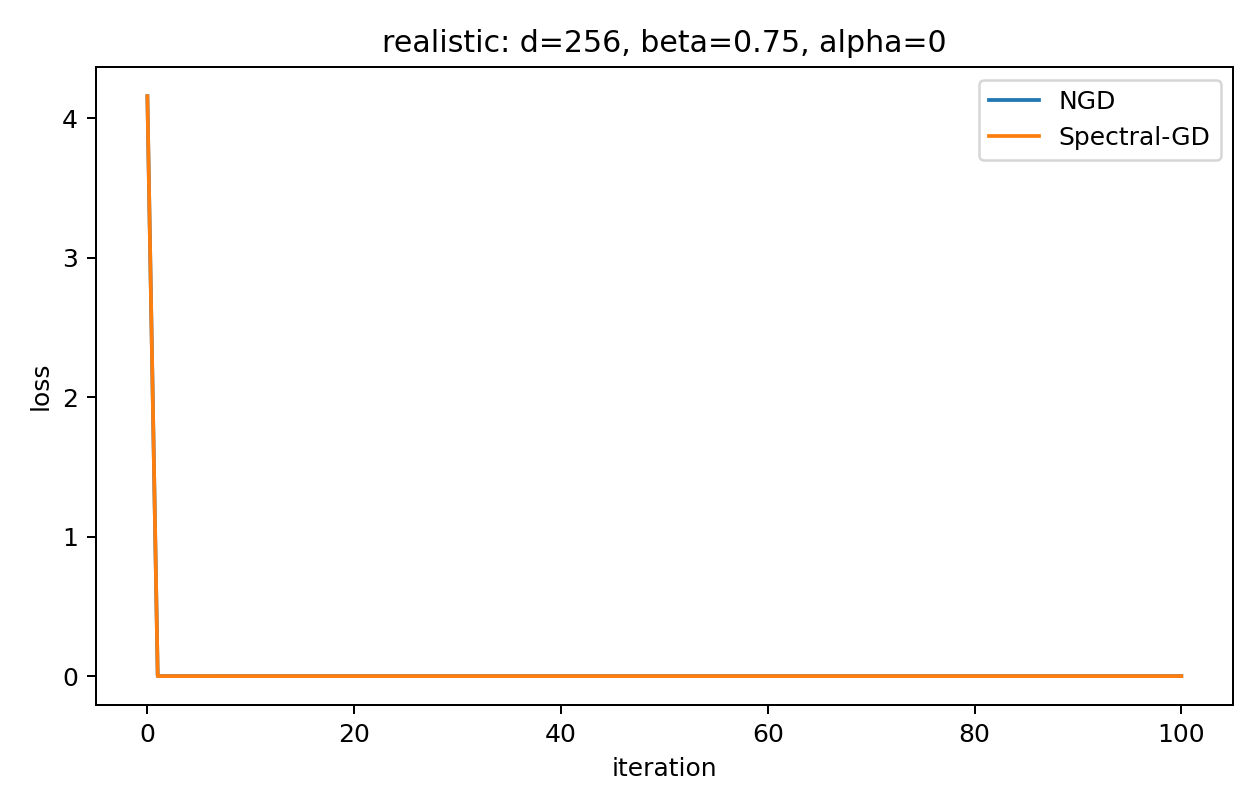
\includegraphics[width=\linewidth]{figures/loss_curves/realistic_d256_b0.75_a0.png}
\caption{$\alpha=0$}
\end{subfigure}%
\hfill
\begin{subfigure}{0.22\textwidth}
\centering
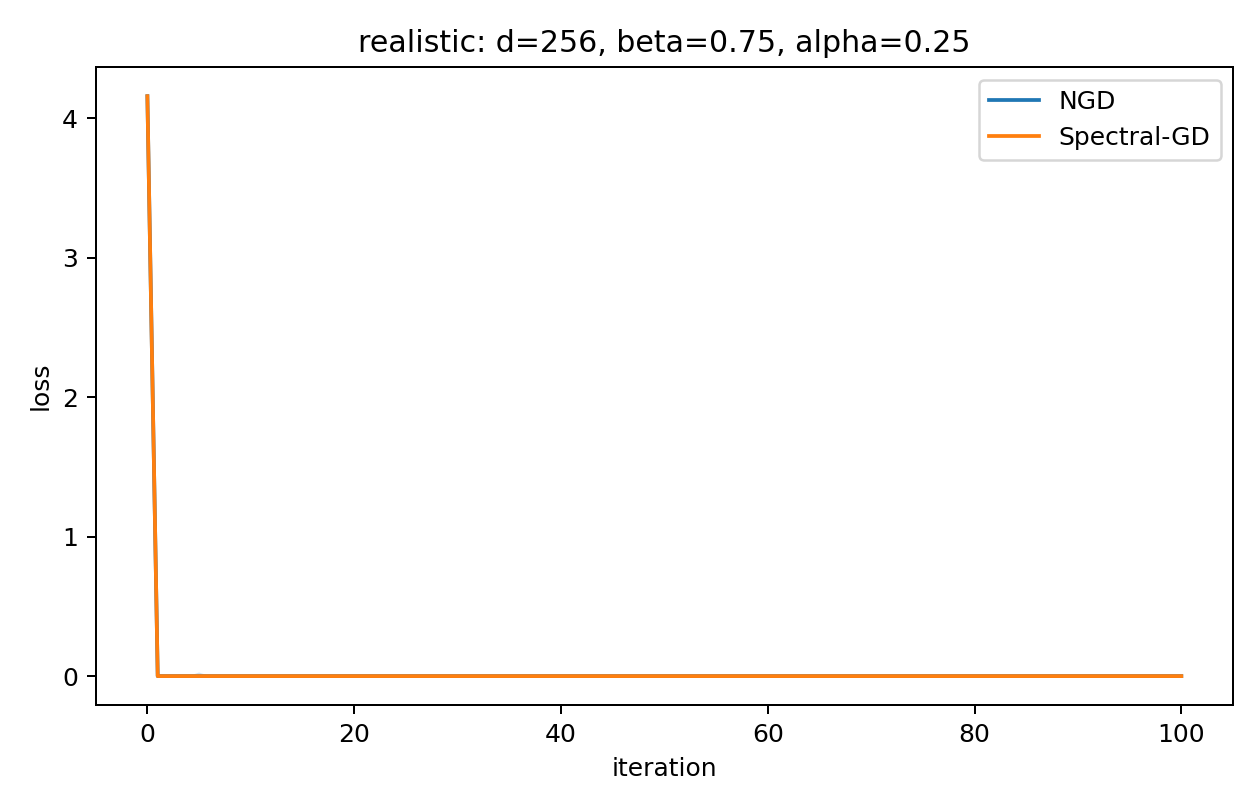
\includegraphics[width=\linewidth]{figures/loss_curves/realistic_d256_b0.75_a0.25.png}
\caption{$\alpha=0.25$}
\end{subfigure}%
\hfill
\begin{subfigure}{0.22\textwidth}
\centering
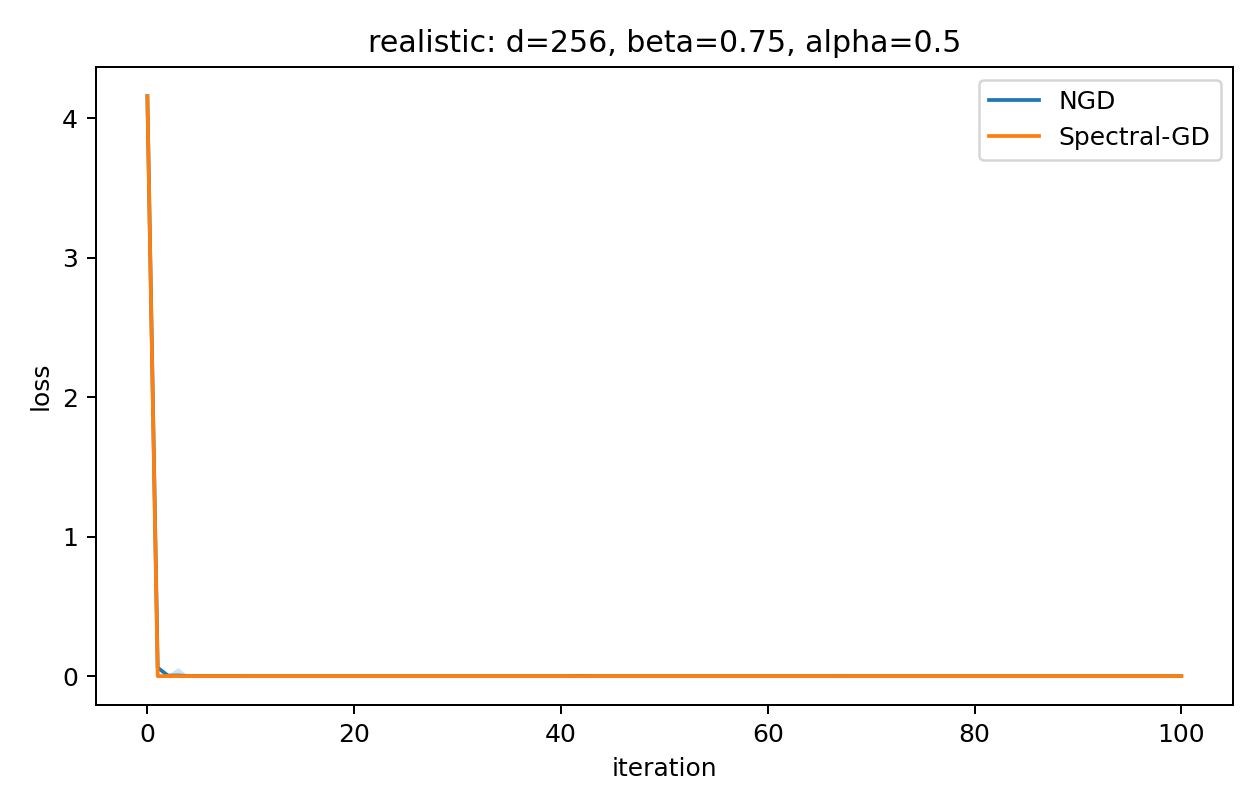
\includegraphics[width=\linewidth]{figures/loss_curves/realistic_d256_b0.75_a0.5.png}
\caption{$\alpha=0.5$}
\end{subfigure}%
\hfill
\begin{subfigure}{0.22\textwidth}
\centering
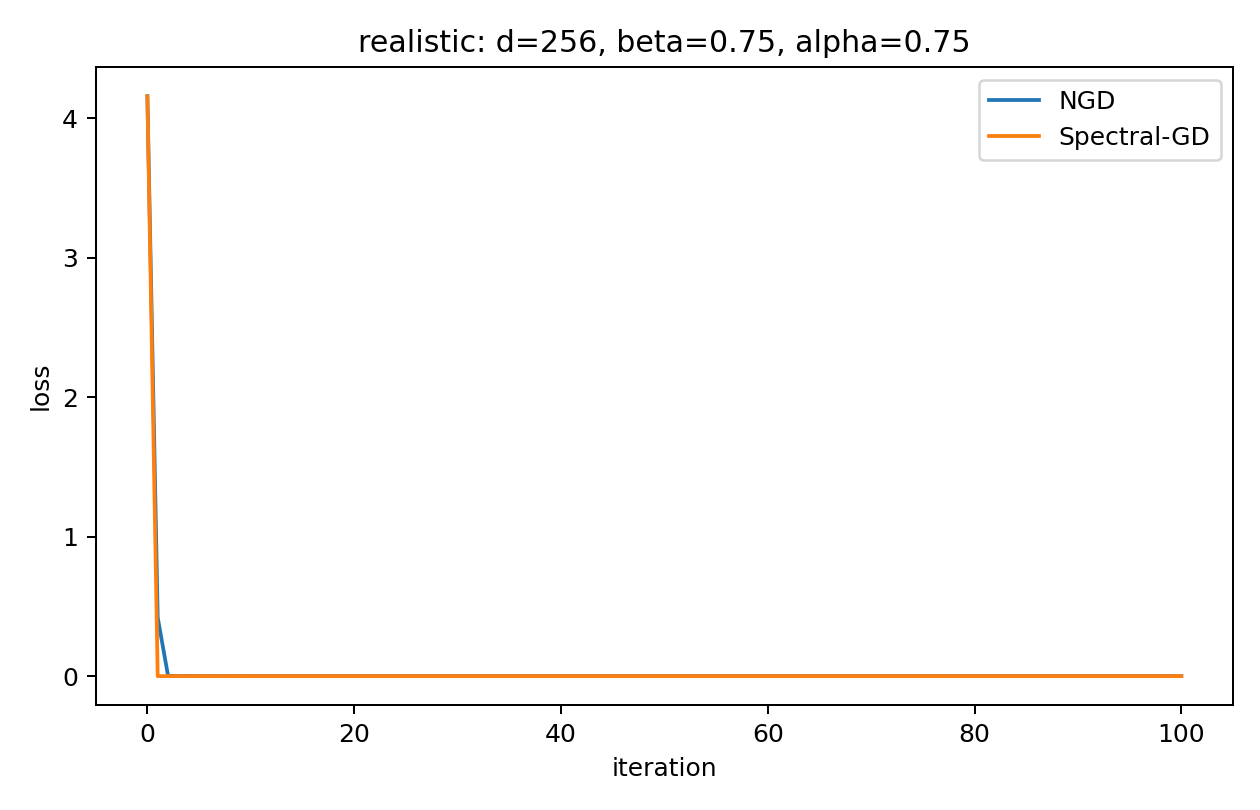
\includegraphics[width=\linewidth]{figures/loss_curves/realistic_d256_b0.75_a0.75.png}
\caption{$\alpha=0.75$}
\end{subfigure}%
\par\smallskip
\begin{subfigure}{0.22\textwidth}
\centering
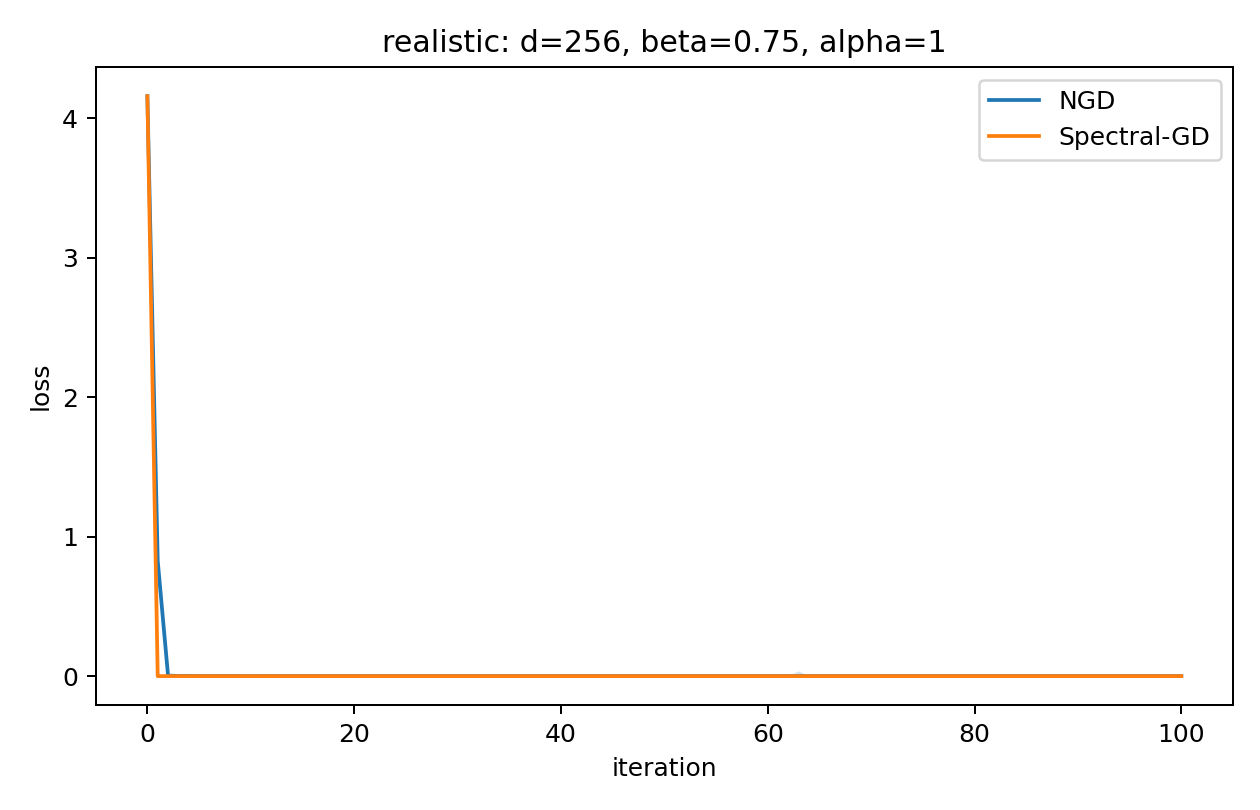
\includegraphics[width=\linewidth]{figures/loss_curves/realistic_d256_b0.75_a1.png}
\caption{$\alpha=1$}
\end{subfigure}%
\hfill
\begin{subfigure}{0.22\textwidth}
\centering
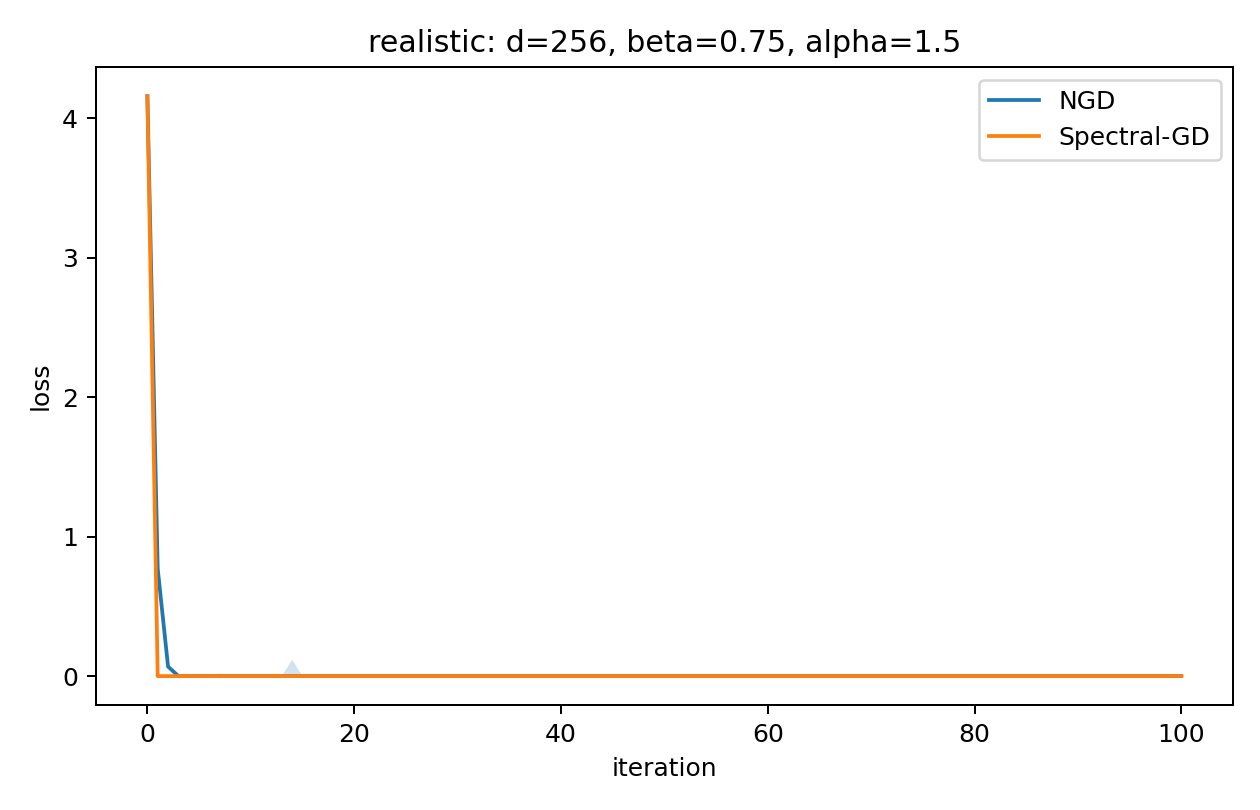
\includegraphics[width=\linewidth]{figures/loss_curves/realistic_d256_b0.75_a1.5.png}
\caption{$\alpha=1.5$}
\end{subfigure}%
\hfill
\begin{subfigure}{0.22\textwidth}
\centering
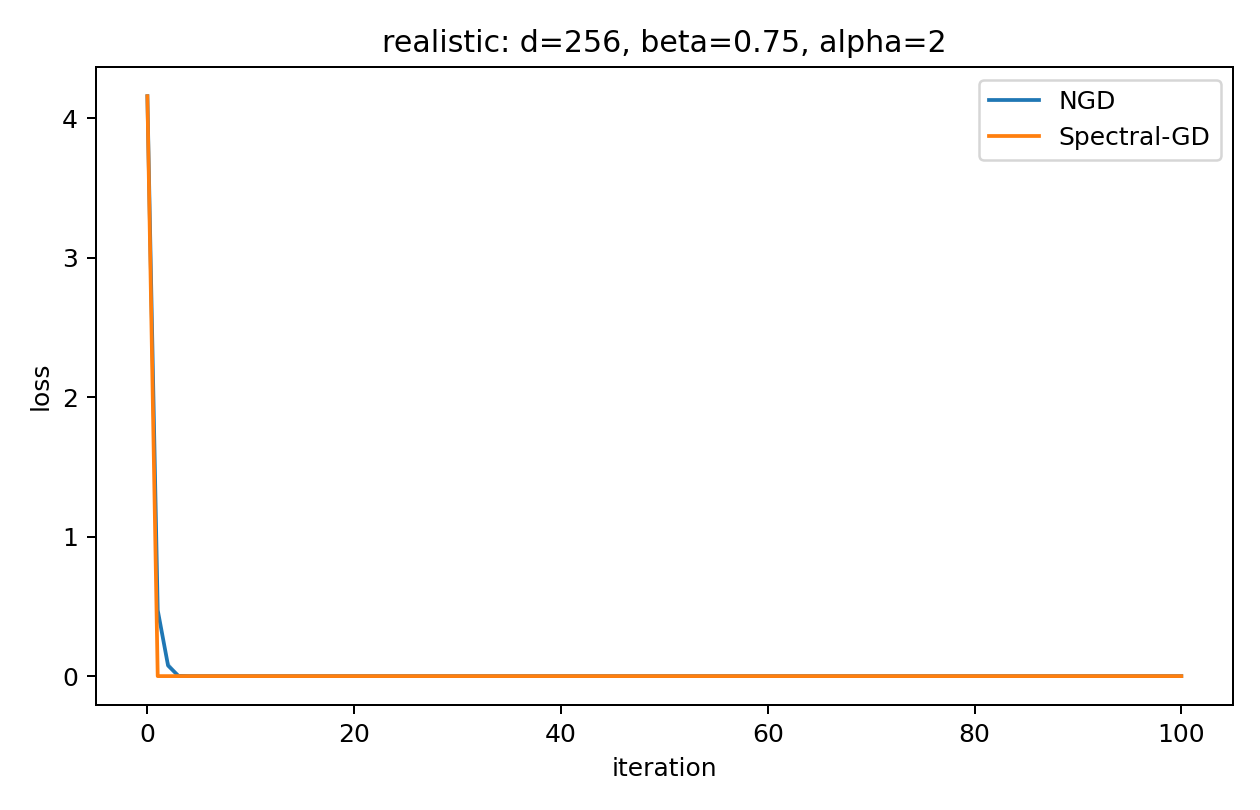
\includegraphics[width=\linewidth]{figures/loss_curves/realistic_d256_b0.75_a2.png}
\caption{$\alpha=2$}
\end{subfigure}%
\caption{Best-auc loss curves for realistic training, $\beta=0.75$, $d=256$, $N=64$. Each panel is one value of $\alpha$. The solid line is the seed median and the shaded band is the interquartile range over three seeds.}
\label{fig:realistic:loss:b075}
\end{figure}


\begin{figure}[H]
\centering
\begin{subfigure}{0.22\textwidth}
\centering

\includegraphics[width=\linewidth]{figures/loss_envelope_curves/realistic_d256_b0.75_a0.png}
\caption{$\alpha=0$}
\end{subfigure}%
\hfill
\begin{subfigure}{0.22\textwidth}
\centering

\includegraphics[width=\linewidth]{figures/loss_envelope_curves/realistic_d256_b0.75_a0.25.png}
\caption{$\alpha=0.25$}
\end{subfigure}%
\hfill
\begin{subfigure}{0.22\textwidth}
\centering

\includegraphics[width=\linewidth]{figures/loss_envelope_curves/realistic_d256_b0.75_a0.5.png}
\caption{$\alpha=0.5$}
\end{subfigure}%
\hfill
\begin{subfigure}{0.22\textwidth}
\centering

\includegraphics[width=\linewidth]{figures/loss_envelope_curves/realistic_d256_b0.75_a0.75.png}
\caption{$\alpha=0.75$}
\end{subfigure}%
\par\smallskip
\begin{subfigure}{0.22\textwidth}
\centering

\includegraphics[width=\linewidth]{figures/loss_envelope_curves/realistic_d256_b0.75_a1.png}
\caption{$\alpha=1$}
\end{subfigure}%
\hfill
\begin{subfigure}{0.22\textwidth}
\centering

\includegraphics[width=\linewidth]{figures/loss_envelope_curves/realistic_d256_b0.75_a1.5.png}
\caption{$\alpha=1.5$}
\end{subfigure}%
\hfill
\begin{subfigure}{0.22\textwidth}
\centering

\includegraphics[width=\linewidth]{figures/loss_envelope_curves/realistic_d256_b0.75_a2.png}
\caption{$\alpha=2$}
\end{subfigure}%
\caption{Loss envelope curves for realistic training, $\beta=0.75$, $d=256$, $N=64$. Each panel is one value of $\alpha$. The solid line is the seed median and the shaded band is the interquartile range over three seeds.}
\label{fig:realistic:envelope:b075}
\end{figure}


\begin{figure}[H]
\centering
\begin{subfigure}{0.22\textwidth}
\centering
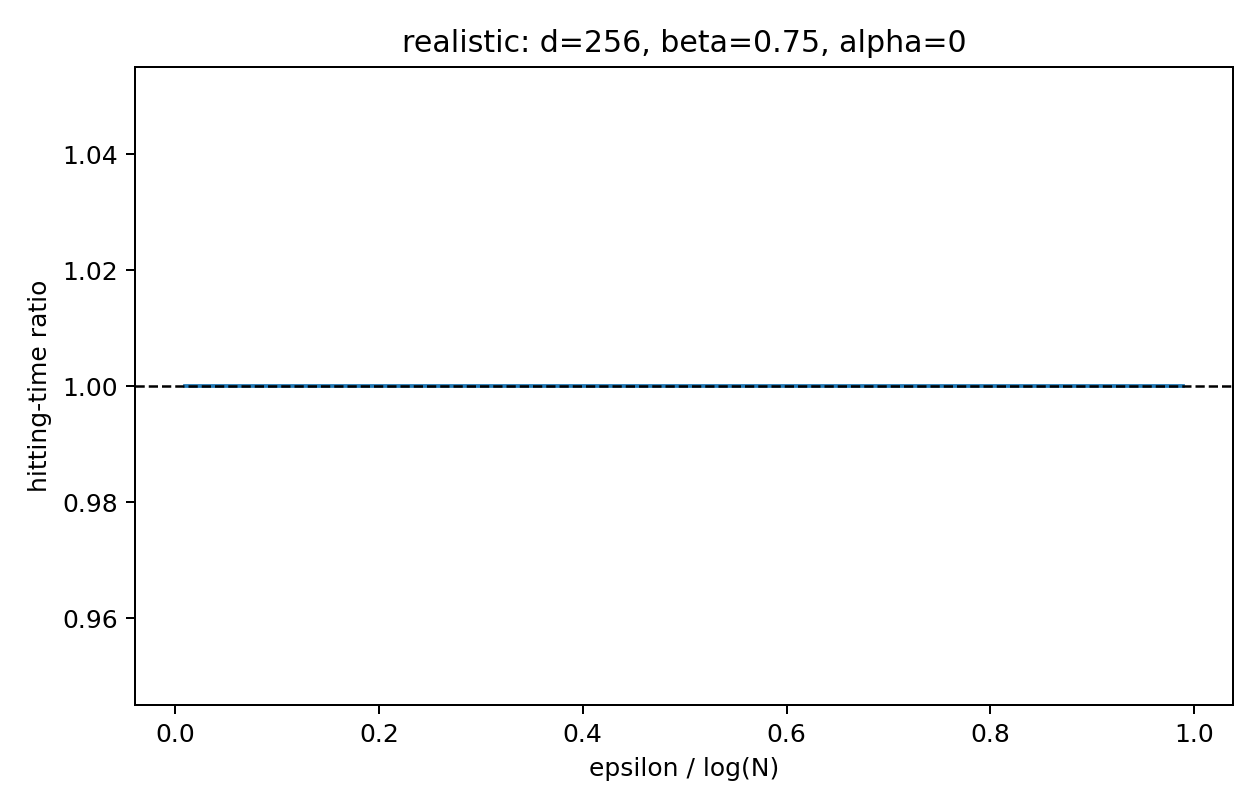
\includegraphics[width=\linewidth]{figures/ratio_curves/T_ratio_realistic_d256_b0.75_a0.png}
\caption{$\alpha=0$}
\end{subfigure}%
\hfill
\begin{subfigure}{0.22\textwidth}
\centering
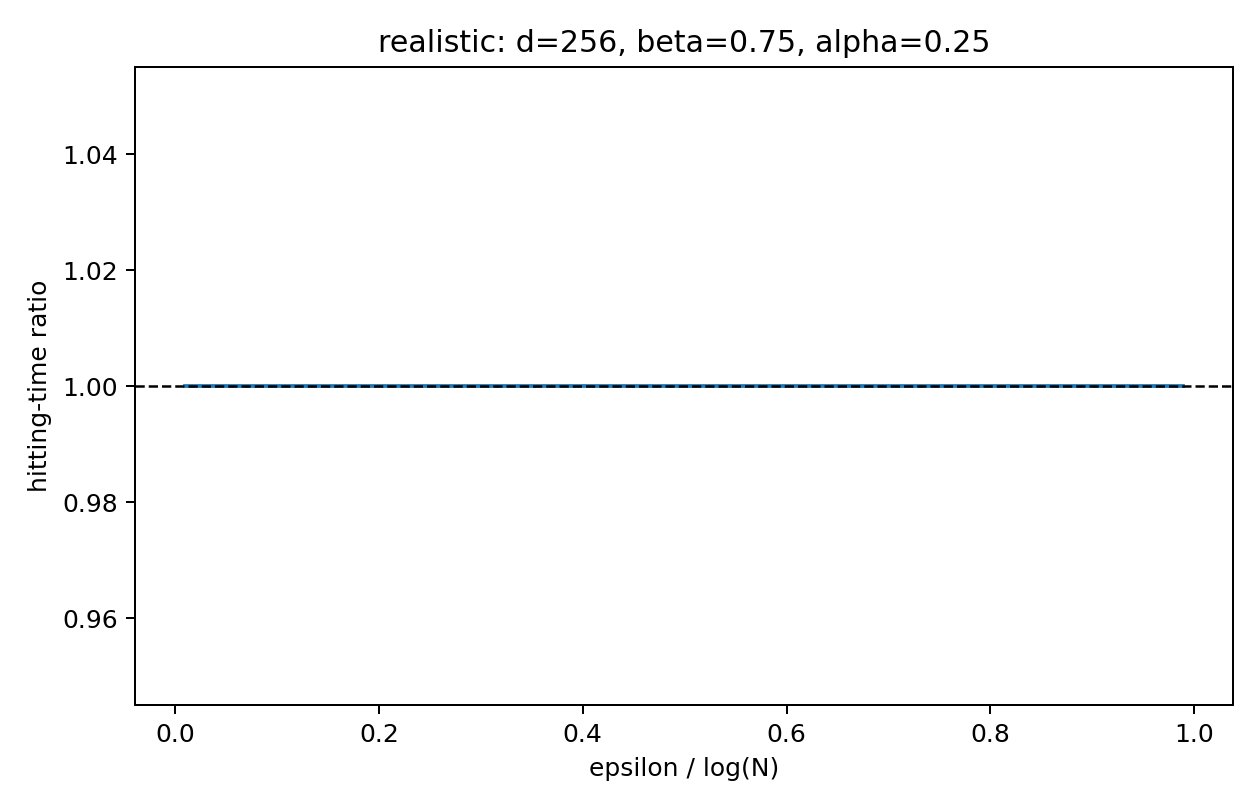
\includegraphics[width=\linewidth]{figures/ratio_curves/T_ratio_realistic_d256_b0.75_a0.25.png}
\caption{$\alpha=0.25$}
\end{subfigure}%
\hfill
\begin{subfigure}{0.22\textwidth}
\centering
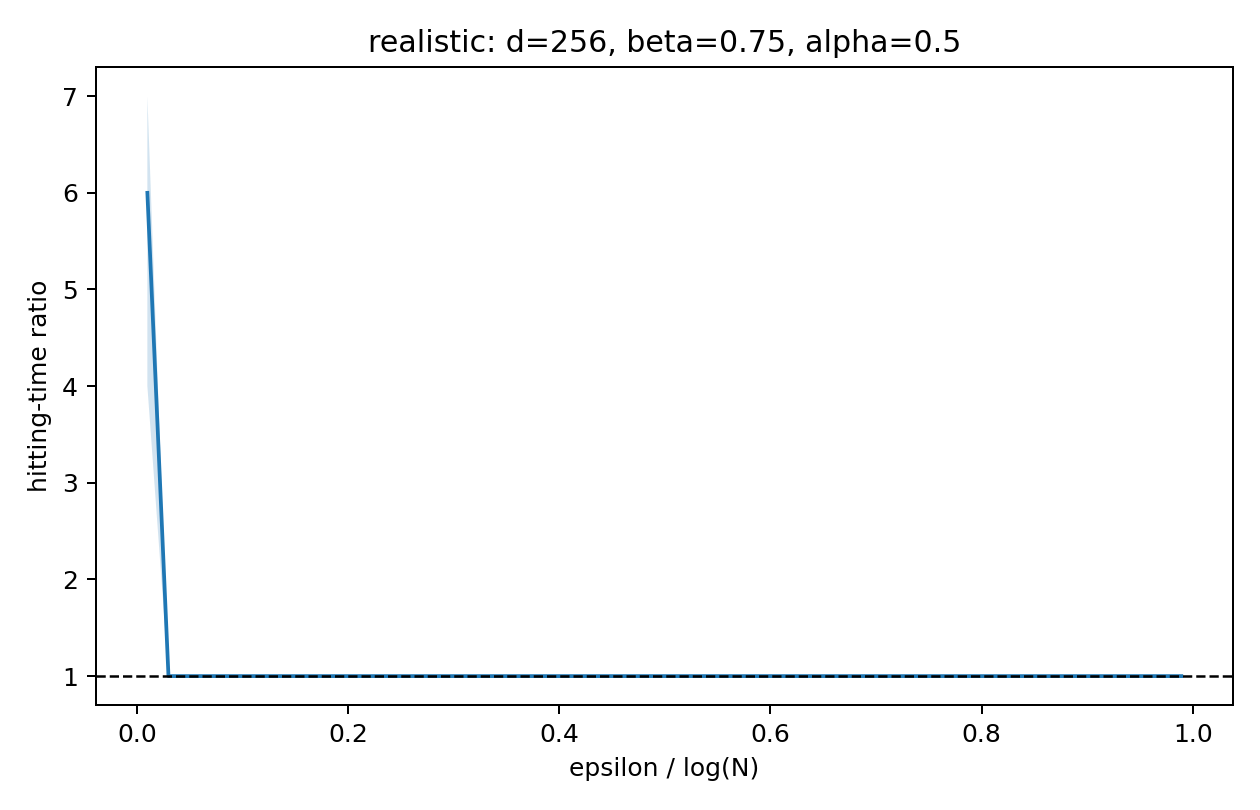
\includegraphics[width=\linewidth]{figures/ratio_curves/T_ratio_realistic_d256_b0.75_a0.5.png}
\caption{$\alpha=0.5$}
\end{subfigure}%
\hfill
\begin{subfigure}{0.22\textwidth}
\centering
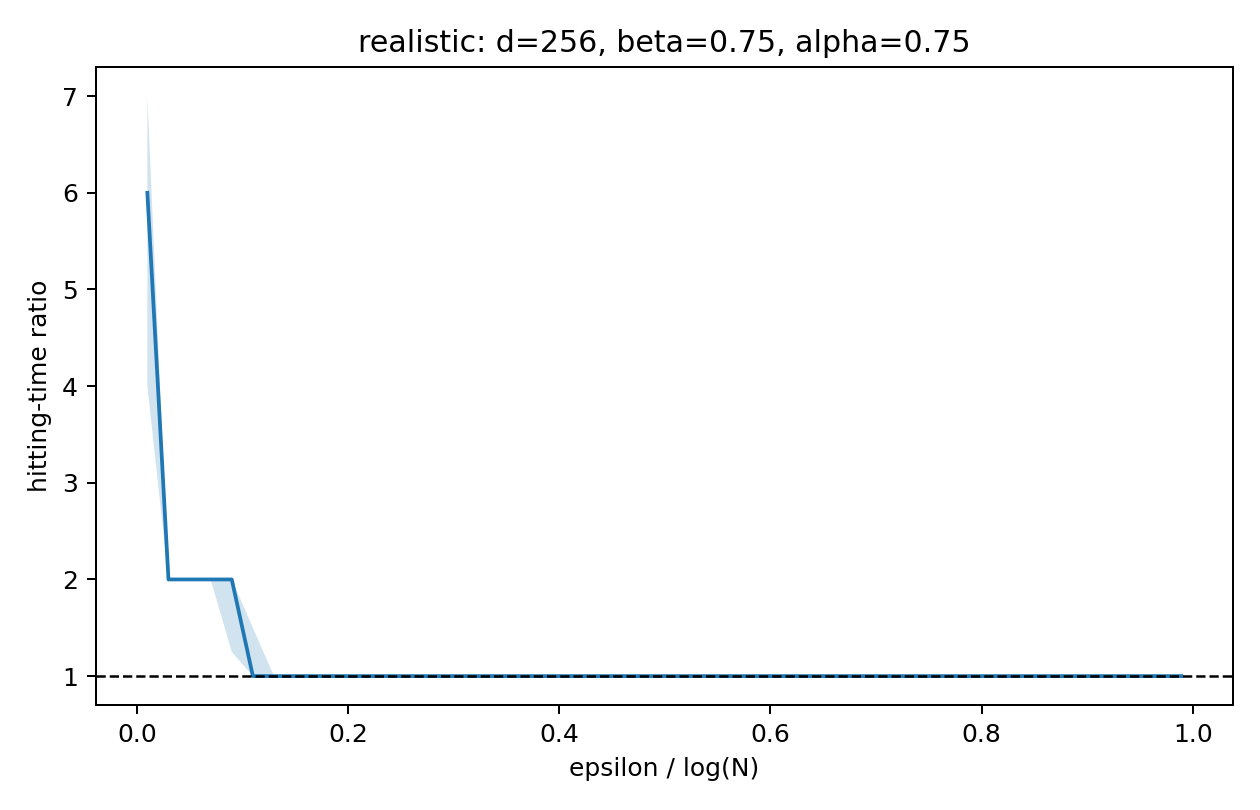
\includegraphics[width=\linewidth]{figures/ratio_curves/T_ratio_realistic_d256_b0.75_a0.75.png}
\caption{$\alpha=0.75$}
\end{subfigure}%
\par\smallskip
\begin{subfigure}{0.22\textwidth}
\centering
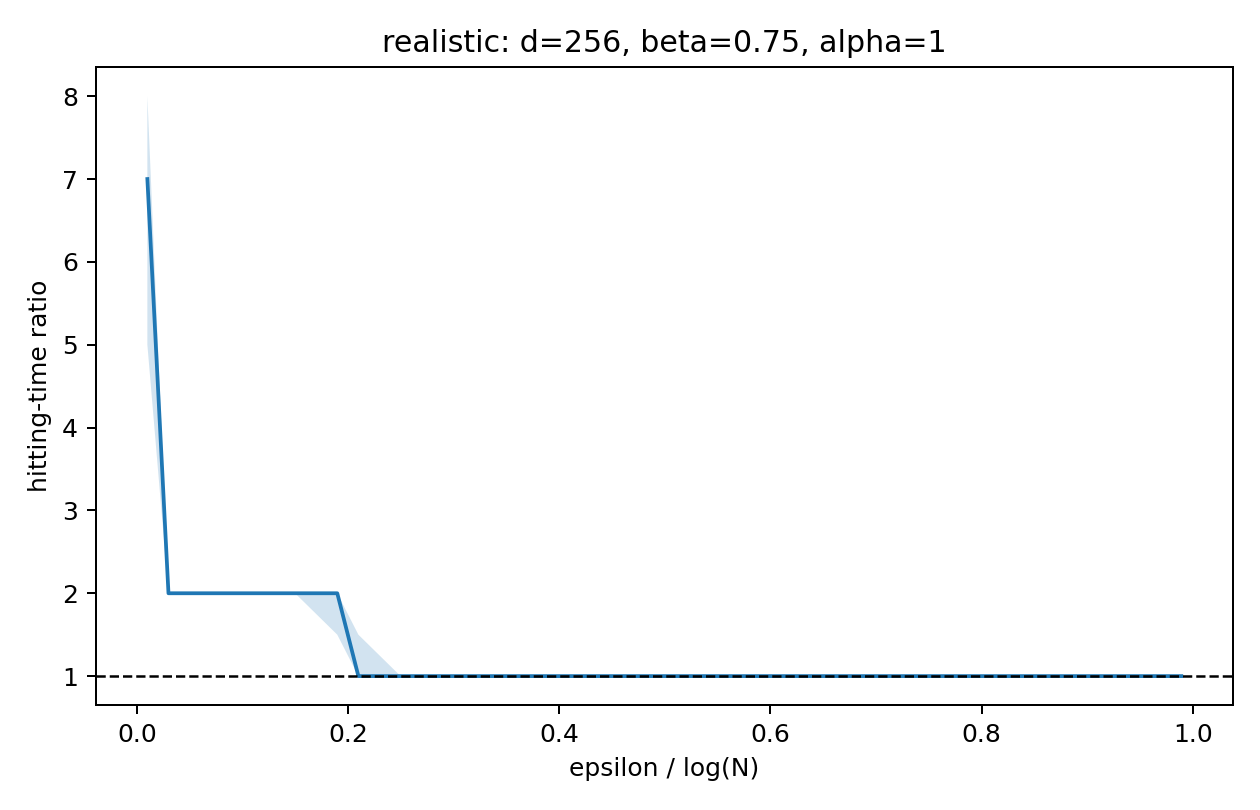
\includegraphics[width=\linewidth]{figures/ratio_curves/T_ratio_realistic_d256_b0.75_a1.png}
\caption{$\alpha=1$}
\end{subfigure}%
\hfill
\begin{subfigure}{0.22\textwidth}
\centering
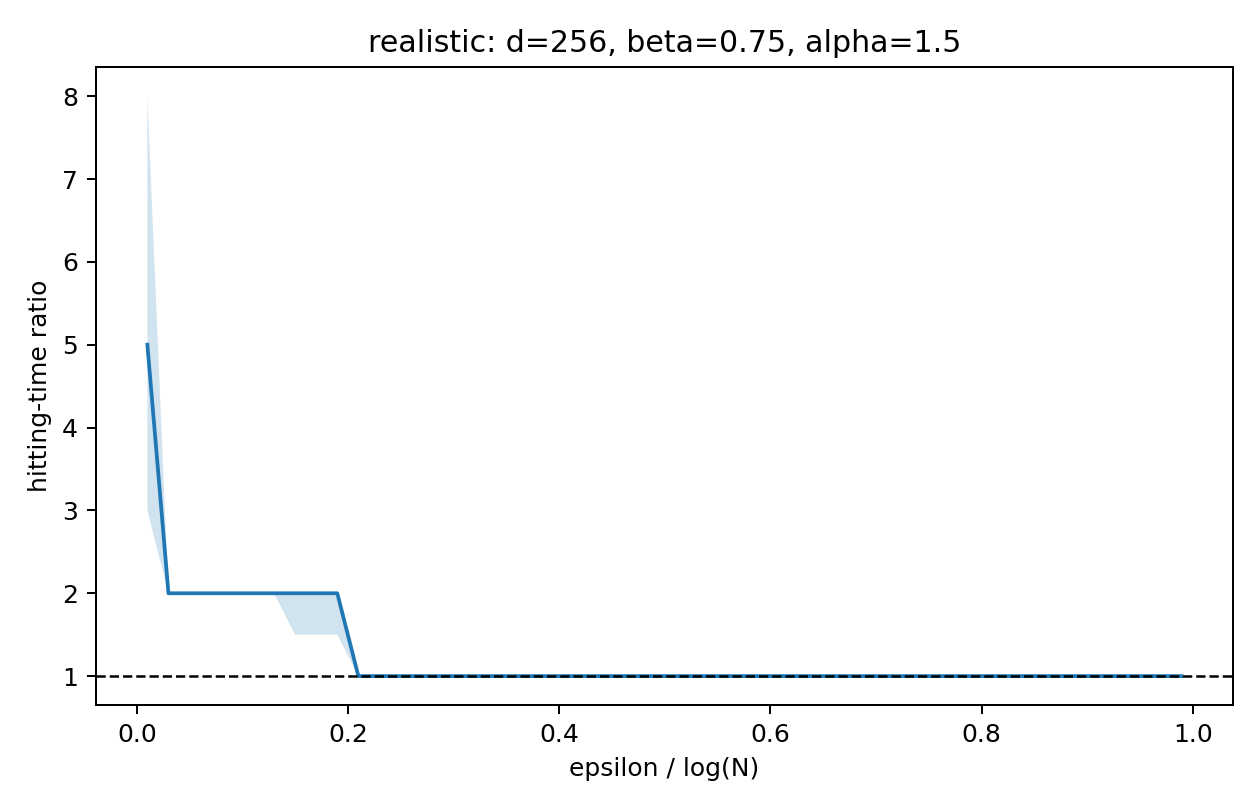
\includegraphics[width=\linewidth]{figures/ratio_curves/T_ratio_realistic_d256_b0.75_a1.5.png}
\caption{$\alpha=1.5$}
\end{subfigure}%
\hfill
\begin{subfigure}{0.22\textwidth}
\centering
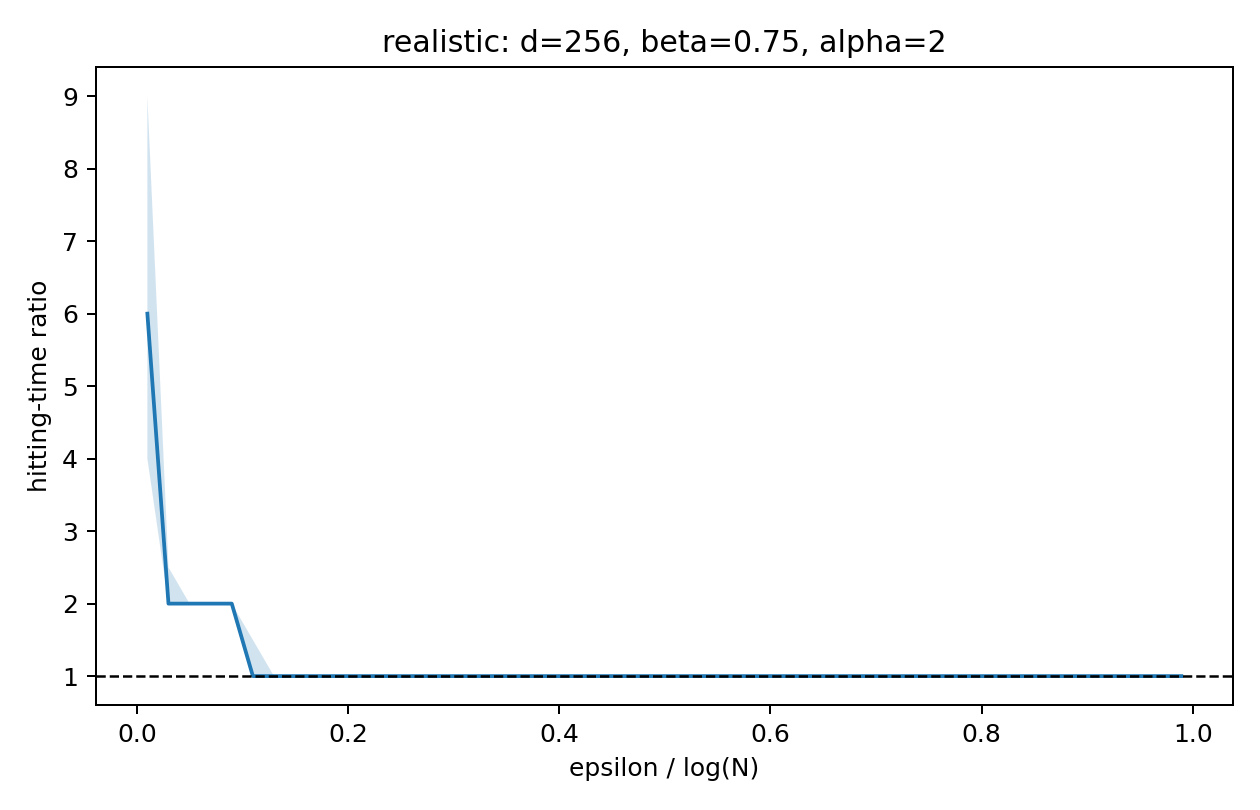
\includegraphics[width=\linewidth]{figures/ratio_curves/T_ratio_realistic_d256_b0.75_a2.png}
\caption{$\alpha=2$}
\end{subfigure}%
\caption{Hitting-time ratio curves for realistic training, $\beta=0.75$, $d=256$, $N=64$. Each panel is one value of $\alpha$. The solid line is the seed median and the shaded band is the interquartile range over three seeds.}
\label{fig:realistic:T_ratio:b075}
\end{figure}






\subsubsection{$\beta=1.25$, $d=256$, $N=1024$}

The following three figures show the complete alpha sweep for this beta block: the best-AUC loss traces, the per-step hyperparameter envelope, and the hitting-time ratio. Reading them together is important: the loss curves show ordinary tuned trajectories, the envelope shows the best loss achievable at each iteration under the sweep, and the hitting-time ratio is the primary speed metric.

\begin{figure}[H]
\centering
\begin{subfigure}{0.22\textwidth}
\centering
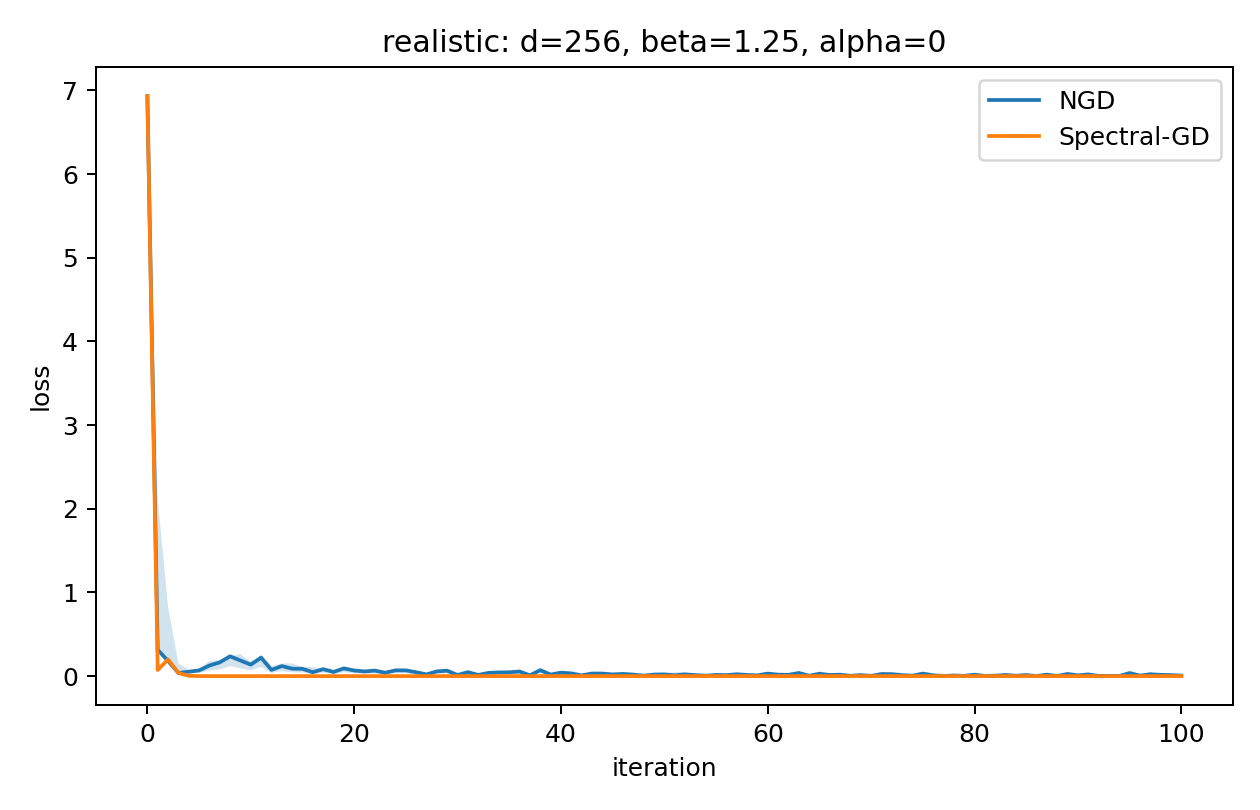
\includegraphics[width=\linewidth]{figures/loss_curves/realistic_d256_b1.25_a0.png}
\caption{$\alpha=0$}
\end{subfigure}%
\hfill
\begin{subfigure}{0.22\textwidth}
\centering
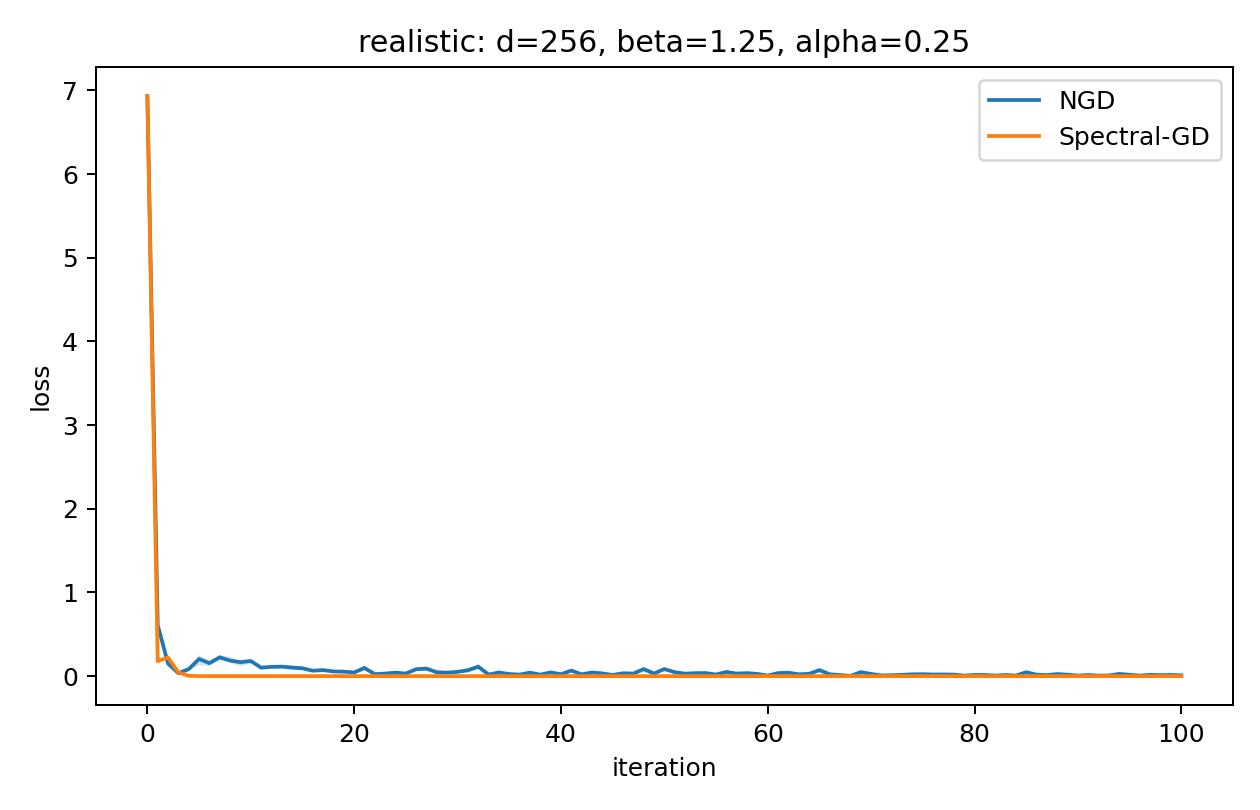
\includegraphics[width=\linewidth]{figures/loss_curves/realistic_d256_b1.25_a0.25.png}
\caption{$\alpha=0.25$}
\end{subfigure}%
\hfill
\begin{subfigure}{0.22\textwidth}
\centering
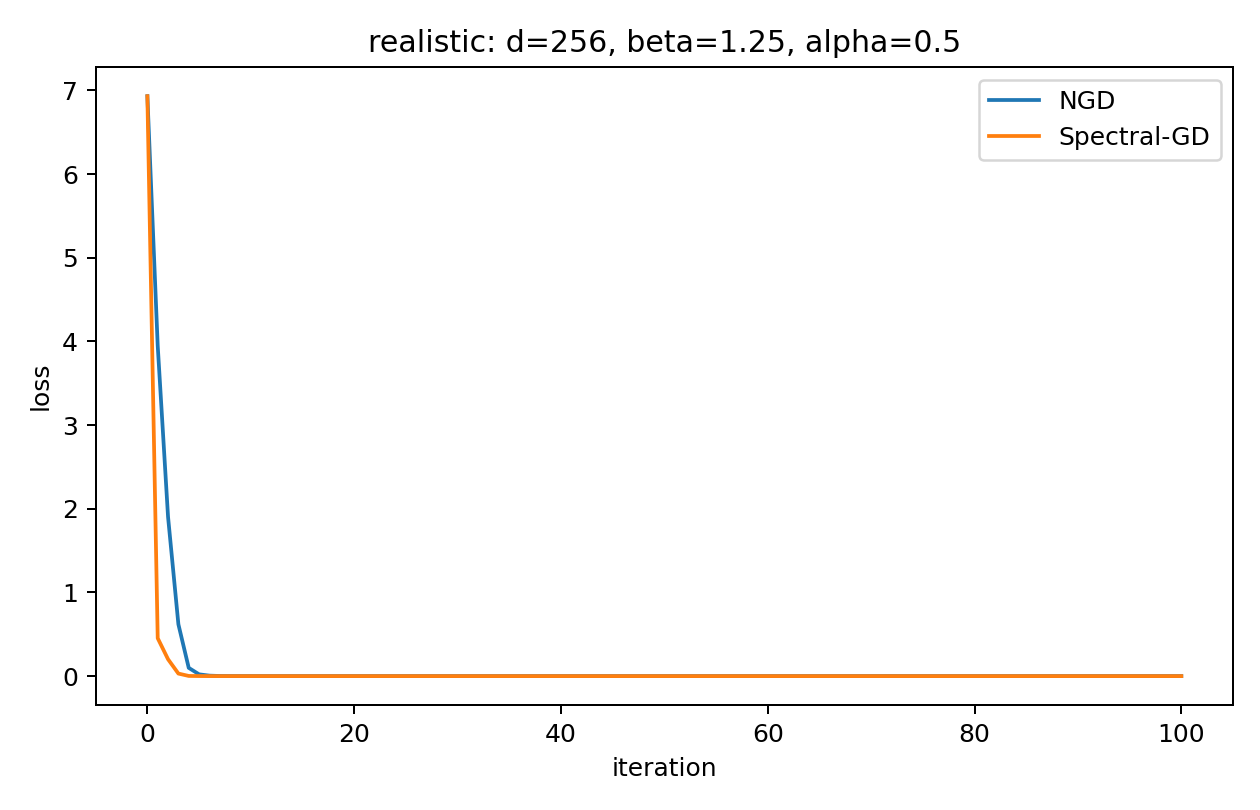
\includegraphics[width=\linewidth]{figures/loss_curves/realistic_d256_b1.25_a0.5.png}
\caption{$\alpha=0.5$}
\end{subfigure}%
\hfill
\begin{subfigure}{0.22\textwidth}
\centering
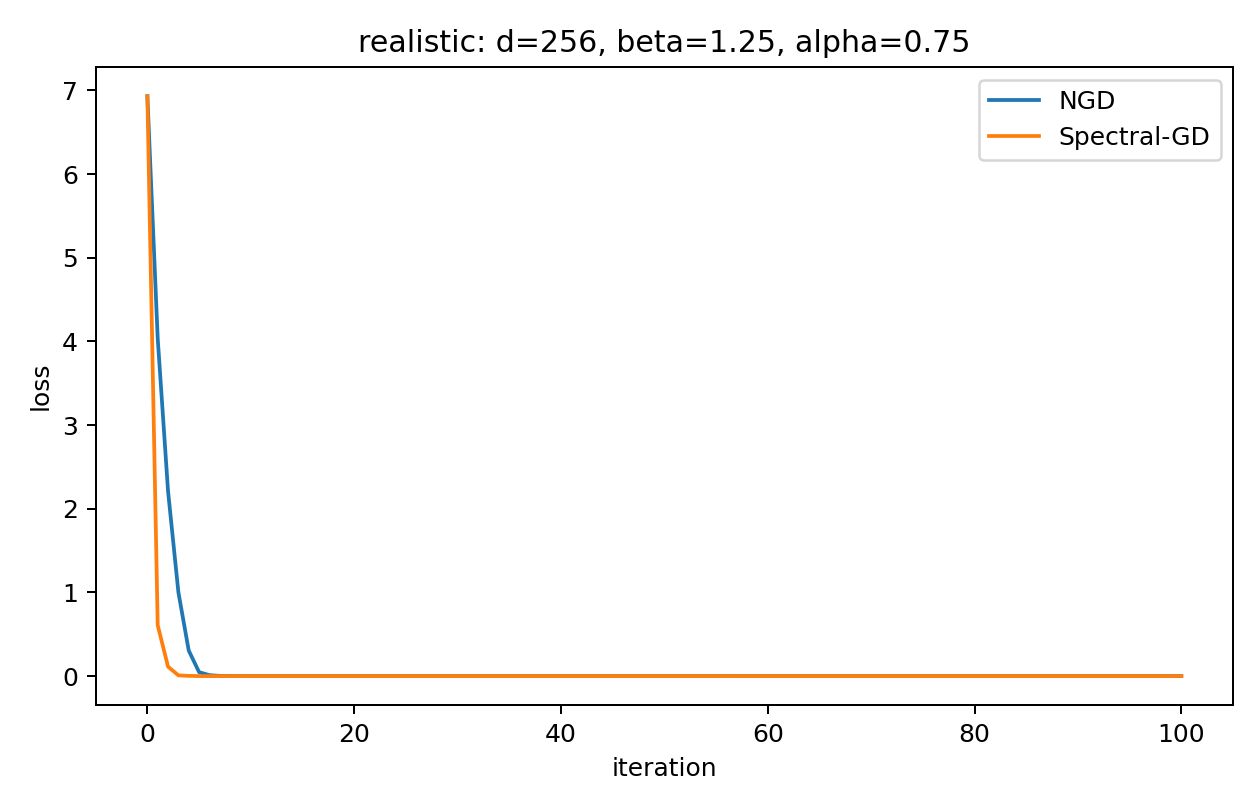
\includegraphics[width=\linewidth]{figures/loss_curves/realistic_d256_b1.25_a0.75.png}
\caption{$\alpha=0.75$}
\end{subfigure}%
\par\smallskip
\begin{subfigure}{0.22\textwidth}
\centering
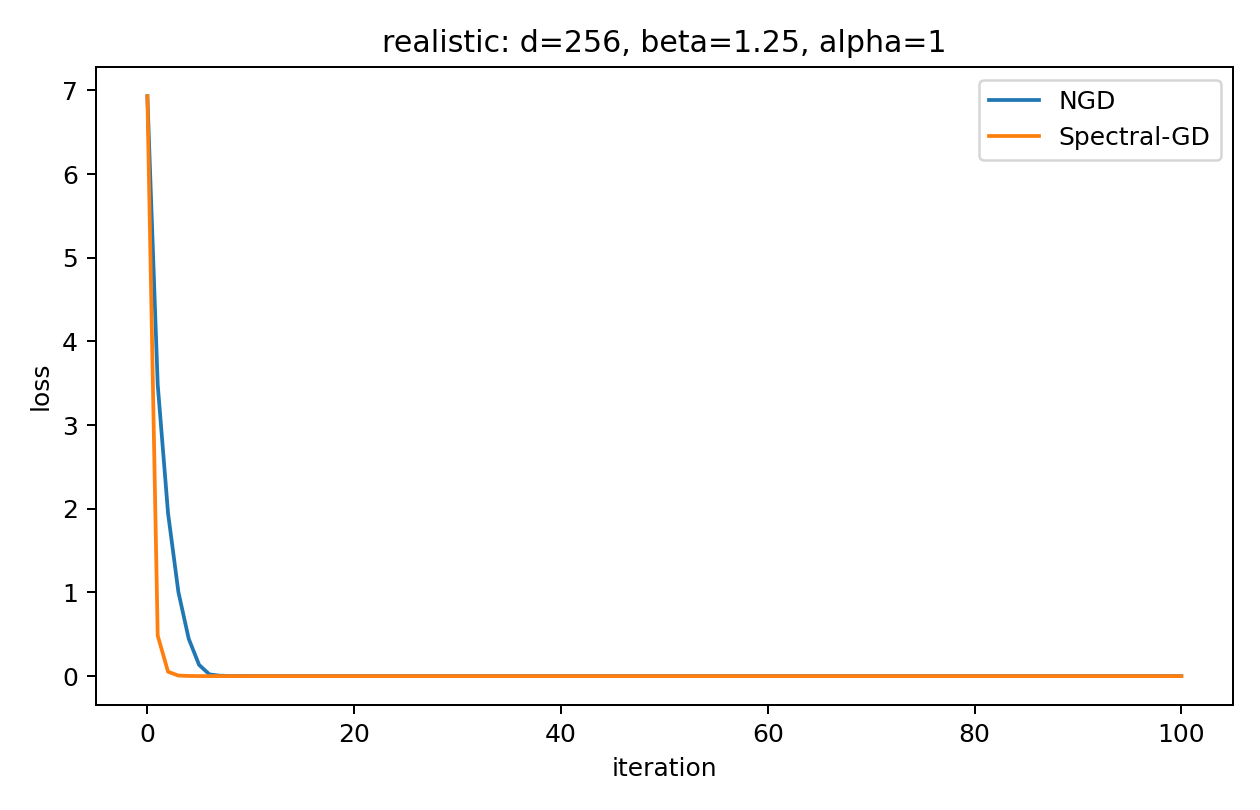
\includegraphics[width=\linewidth]{figures/loss_curves/realistic_d256_b1.25_a1.png}
\caption{$\alpha=1$}
\end{subfigure}%
\hfill
\begin{subfigure}{0.22\textwidth}
\centering
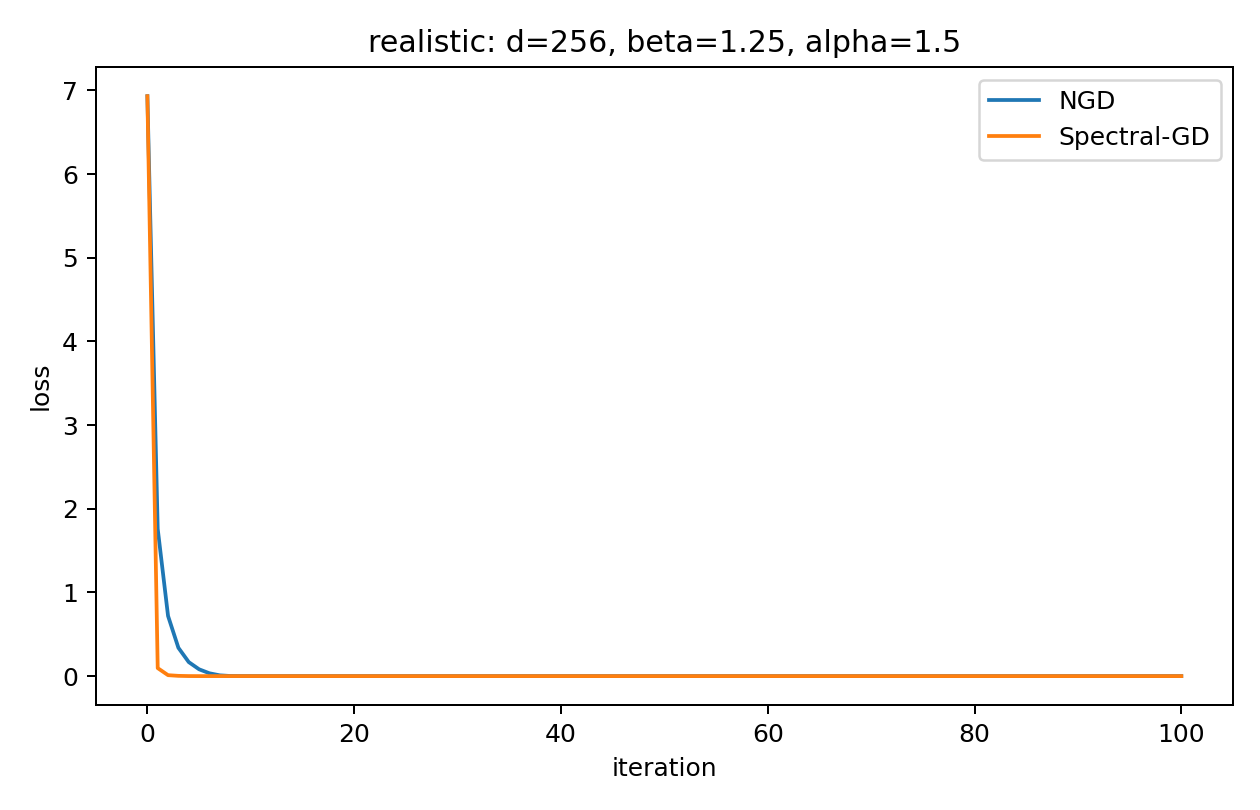
\includegraphics[width=\linewidth]{figures/loss_curves/realistic_d256_b1.25_a1.5.png}
\caption{$\alpha=1.5$}
\end{subfigure}%
\hfill
\begin{subfigure}{0.22\textwidth}
\centering
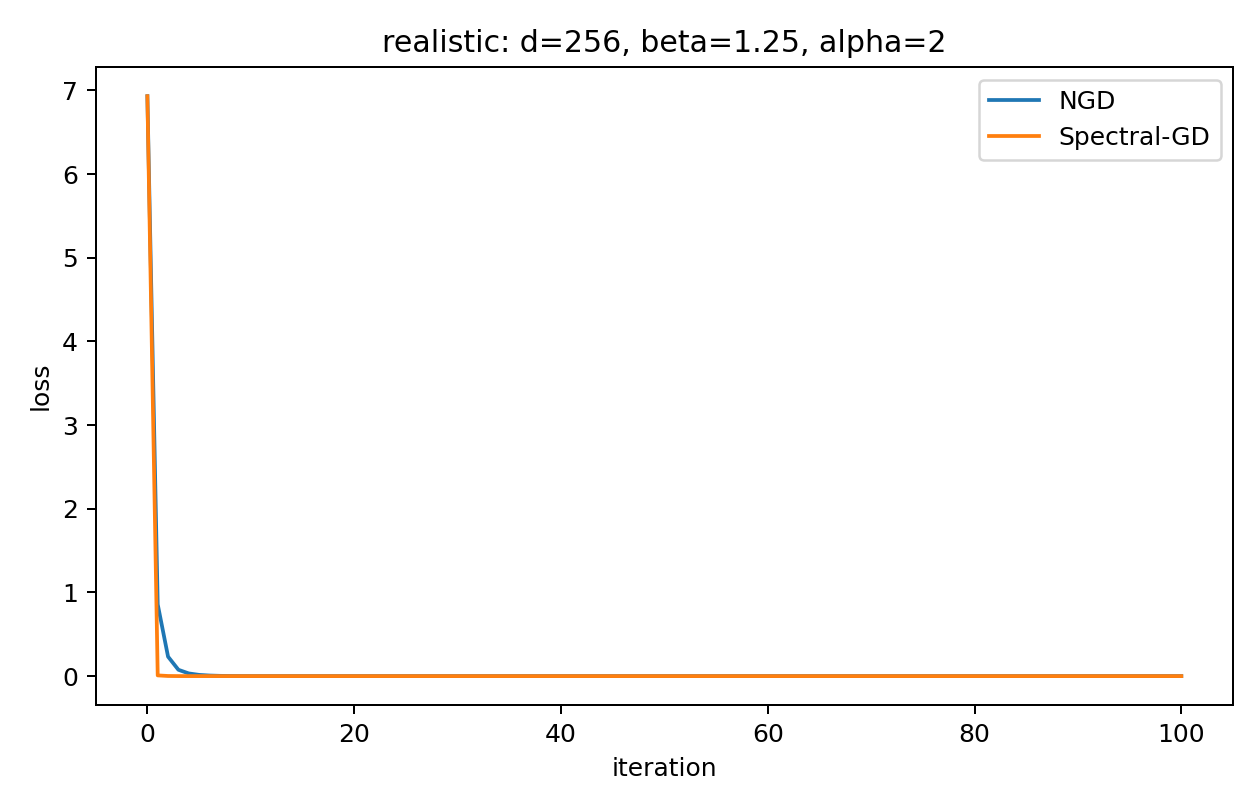
\includegraphics[width=\linewidth]{figures/loss_curves/realistic_d256_b1.25_a2.png}
\caption{$\alpha=2$}
\end{subfigure}%
\caption{Best-auc loss curves for realistic training, $\beta=1.25$, $d=256$, $N=1024$. Each panel is one value of $\alpha$. The solid line is the seed median and the shaded band is the interquartile range over three seeds.}
\label{fig:realistic:loss:b125}
\end{figure}


\begin{figure}[H]
\centering
\begin{subfigure}{0.22\textwidth}
\centering

\includegraphics[width=\linewidth]{figures/loss_envelope_curves/realistic_d256_b1.25_a0.png}
\caption{$\alpha=0$}
\end{subfigure}%
\hfill
\begin{subfigure}{0.22\textwidth}
\centering

\includegraphics[width=\linewidth]{figures/loss_envelope_curves/realistic_d256_b1.25_a0.25.png}
\caption{$\alpha=0.25$}
\end{subfigure}%
\hfill
\begin{subfigure}{0.22\textwidth}
\centering

\includegraphics[width=\linewidth]{figures/loss_envelope_curves/realistic_d256_b1.25_a0.5.png}
\caption{$\alpha=0.5$}
\end{subfigure}%
\hfill
\begin{subfigure}{0.22\textwidth}
\centering

\includegraphics[width=\linewidth]{figures/loss_envelope_curves/realistic_d256_b1.25_a0.75.png}
\caption{$\alpha=0.75$}
\end{subfigure}%
\par\smallskip
\begin{subfigure}{0.22\textwidth}
\centering

\includegraphics[width=\linewidth]{figures/loss_envelope_curves/realistic_d256_b1.25_a1.png}
\caption{$\alpha=1$}
\end{subfigure}%
\hfill
\begin{subfigure}{0.22\textwidth}
\centering

\includegraphics[width=\linewidth]{figures/loss_envelope_curves/realistic_d256_b1.25_a1.5.png}
\caption{$\alpha=1.5$}
\end{subfigure}%
\hfill
\begin{subfigure}{0.22\textwidth}
\centering

\includegraphics[width=\linewidth]{figures/loss_envelope_curves/realistic_d256_b1.25_a2.png}
\caption{$\alpha=2$}
\end{subfigure}%
\caption{Loss envelope curves for realistic training, $\beta=1.25$, $d=256$, $N=1024$. Each panel is one value of $\alpha$. The solid line is the seed median and the shaded band is the interquartile range over three seeds.}
\label{fig:realistic:envelope:b125}
\end{figure}


\begin{figure}[H]
\centering
\begin{subfigure}{0.22\textwidth}
\centering
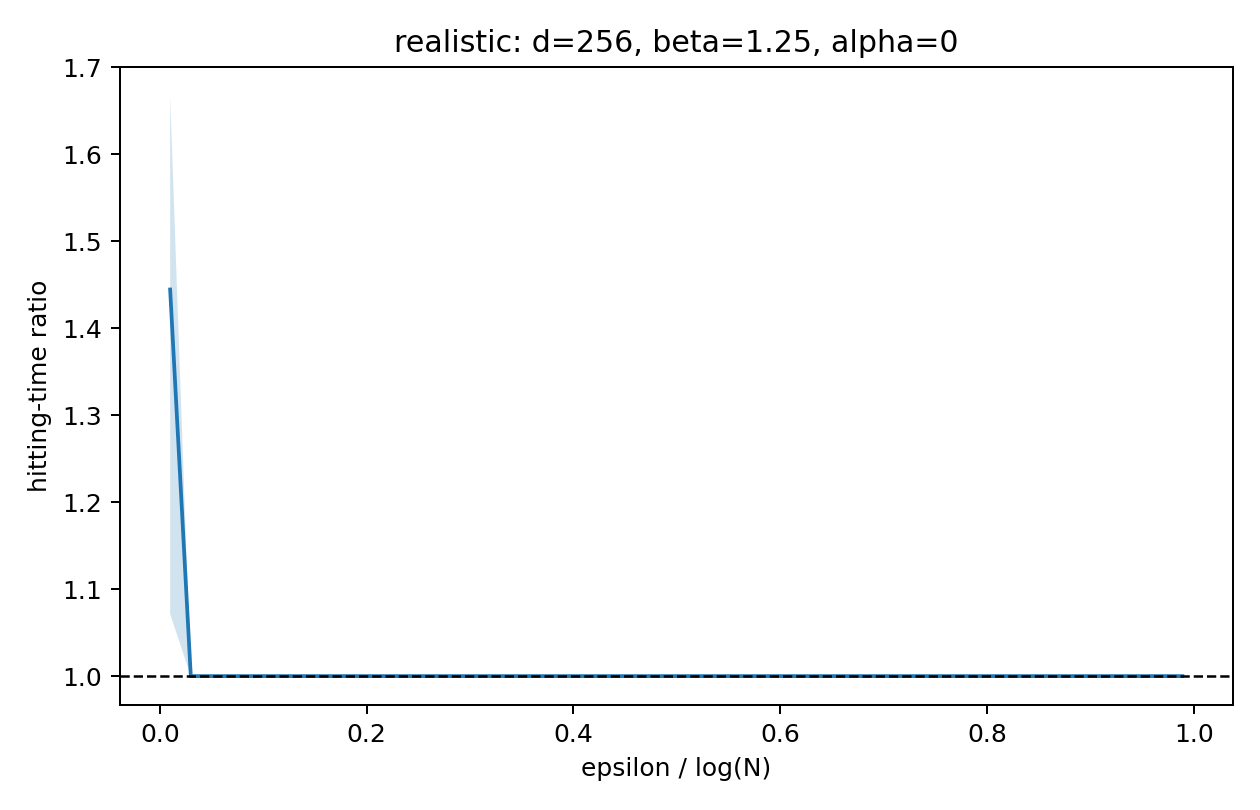
\includegraphics[width=\linewidth]{figures/ratio_curves/T_ratio_realistic_d256_b1.25_a0.png}
\caption{$\alpha=0$}
\end{subfigure}%
\hfill
\begin{subfigure}{0.22\textwidth}
\centering
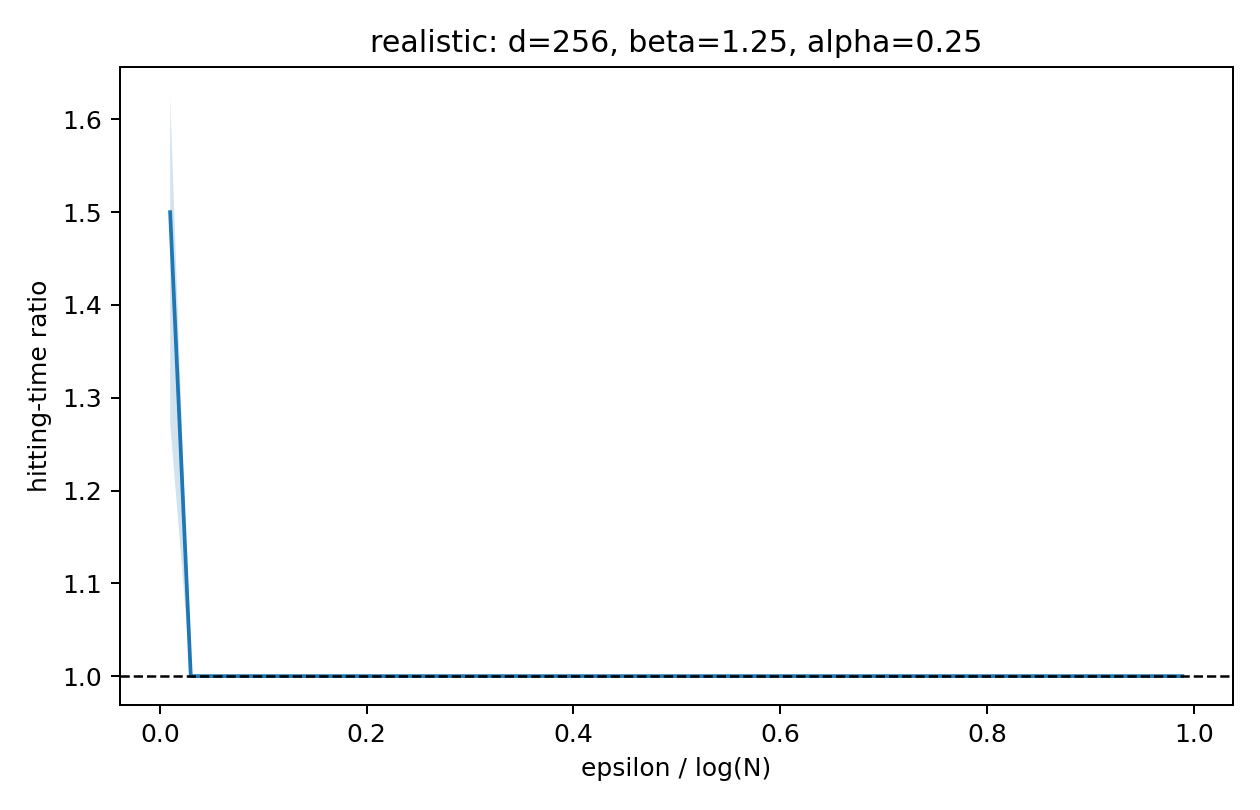
\includegraphics[width=\linewidth]{figures/ratio_curves/T_ratio_realistic_d256_b1.25_a0.25.png}
\caption{$\alpha=0.25$}
\end{subfigure}%
\hfill
\begin{subfigure}{0.22\textwidth}
\centering
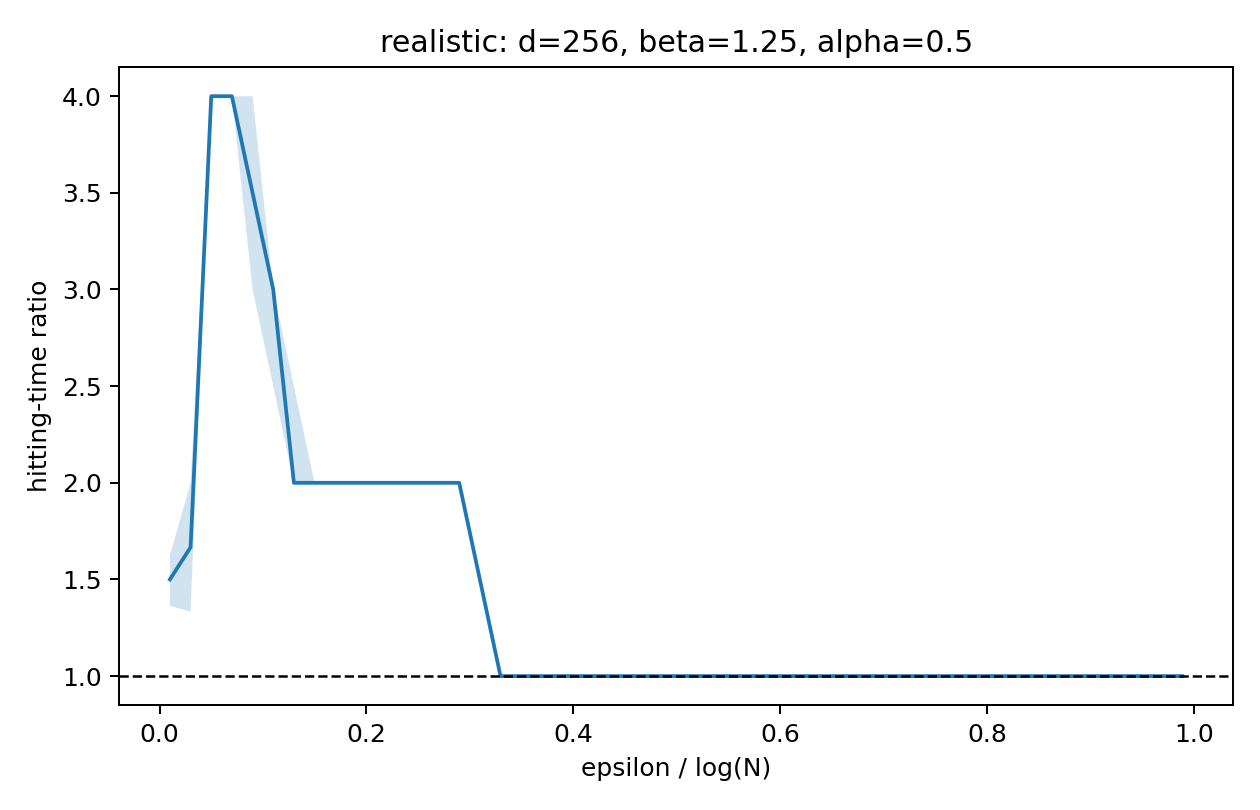
\includegraphics[width=\linewidth]{figures/ratio_curves/T_ratio_realistic_d256_b1.25_a0.5.png}
\caption{$\alpha=0.5$}
\end{subfigure}%
\hfill
\begin{subfigure}{0.22\textwidth}
\centering
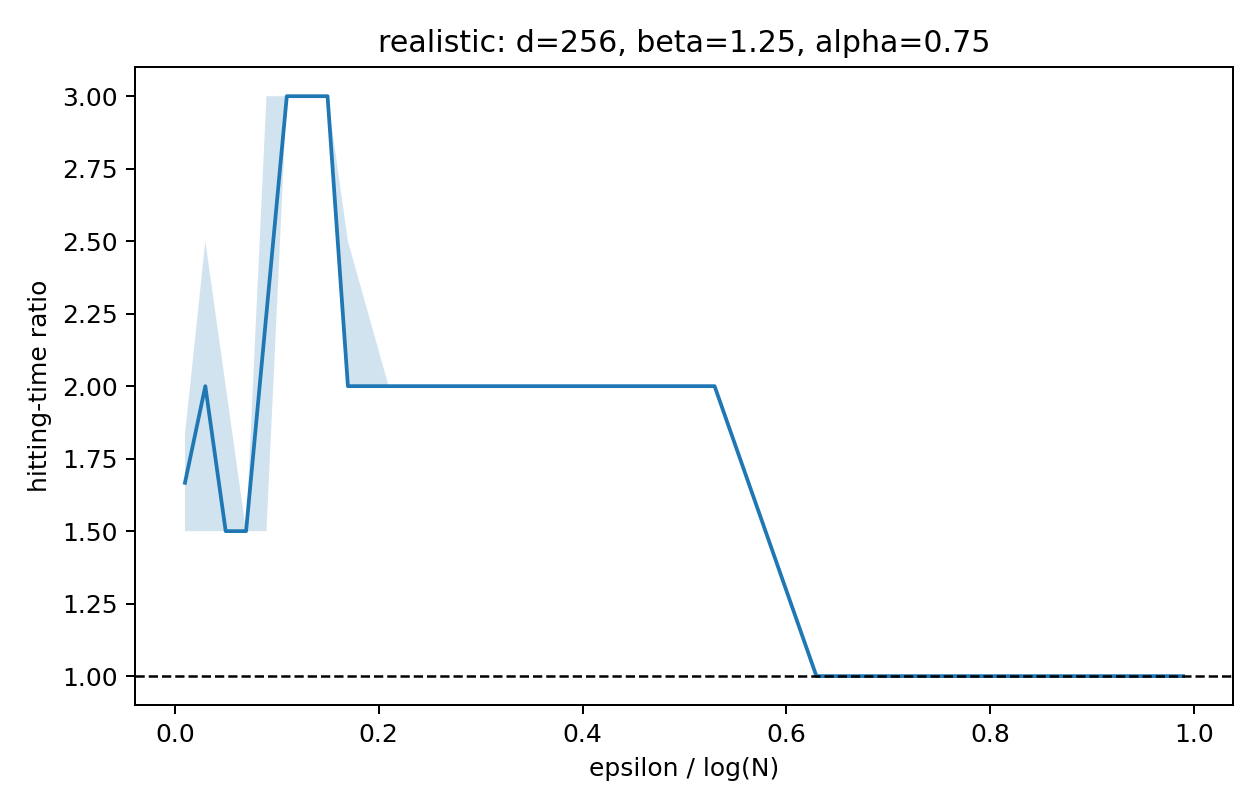
\includegraphics[width=\linewidth]{figures/ratio_curves/T_ratio_realistic_d256_b1.25_a0.75.png}
\caption{$\alpha=0.75$}
\end{subfigure}%
\par\smallskip
\begin{subfigure}{0.22\textwidth}
\centering
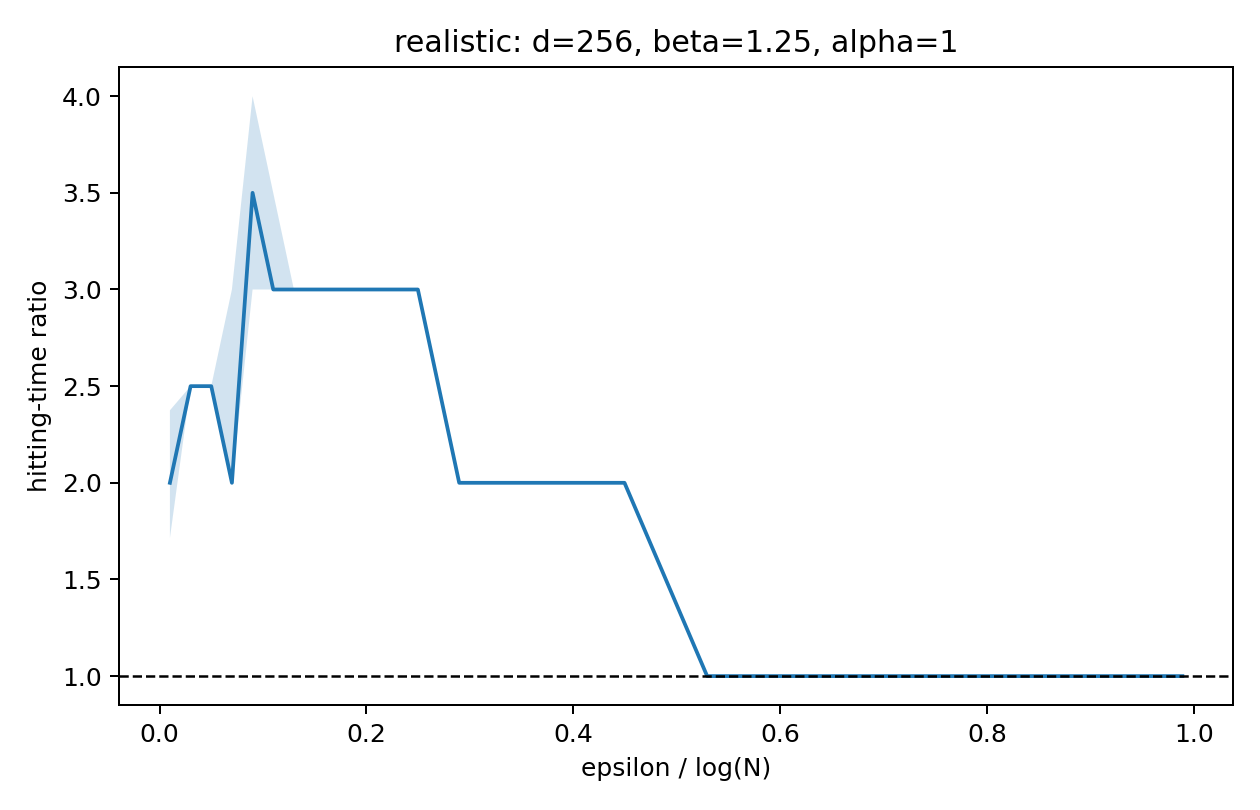
\includegraphics[width=\linewidth]{figures/ratio_curves/T_ratio_realistic_d256_b1.25_a1.png}
\caption{$\alpha=1$}
\end{subfigure}%
\hfill
\begin{subfigure}{0.22\textwidth}
\centering
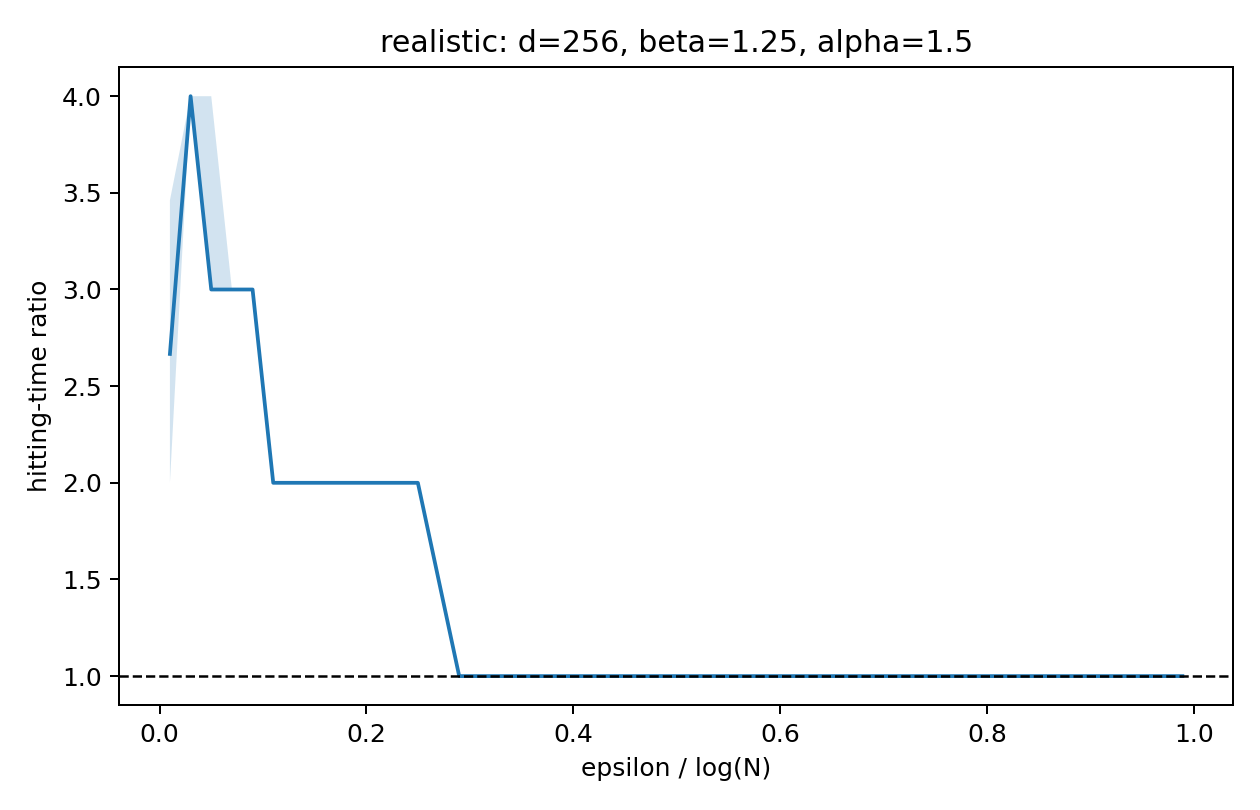
\includegraphics[width=\linewidth]{figures/ratio_curves/T_ratio_realistic_d256_b1.25_a1.5.png}
\caption{$\alpha=1.5$}
\end{subfigure}%
\hfill
\begin{subfigure}{0.22\textwidth}
\centering
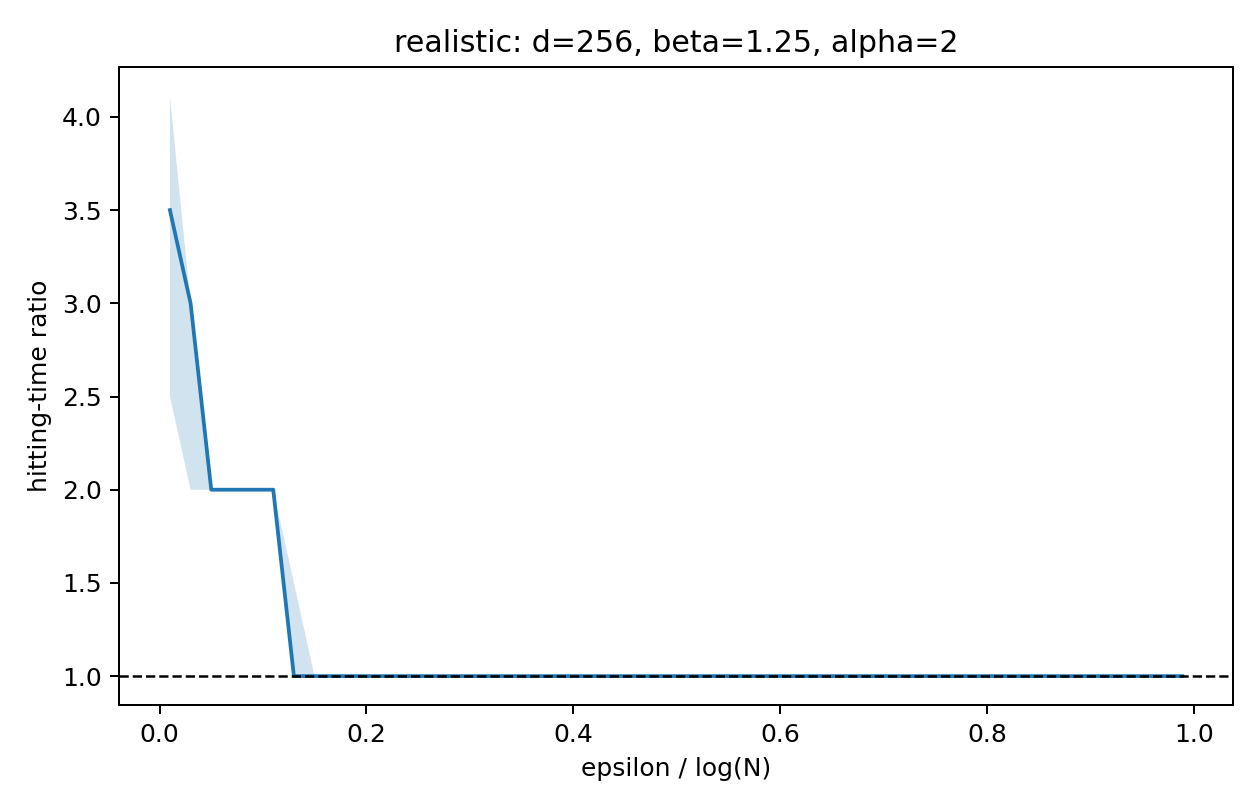
\includegraphics[width=\linewidth]{figures/ratio_curves/T_ratio_realistic_d256_b1.25_a2.png}
\caption{$\alpha=2$}
\end{subfigure}%
\caption{Hitting-time ratio curves for realistic training, $\beta=1.25$, $d=256$, $N=1024$. Each panel is one value of $\alpha$. The solid line is the seed median and the shaded band is the interquartile range over three seeds.}
\label{fig:realistic:T_ratio:b125}
\end{figure}



\subsubsection{$\beta=1.5$, $d=256$, $N=4096$}

The following three figures show the complete alpha sweep for this beta block: the best-AUC loss traces, the per-step hyperparameter envelope, and the hitting-time ratio. Reading them together is important: the loss curves show ordinary tuned trajectories, the envelope shows the best loss achievable at each iteration under the sweep, and the hitting-time ratio is the primary speed metric.

\begin{figure}[H]
\centering
\begin{subfigure}{0.22\textwidth}
\centering
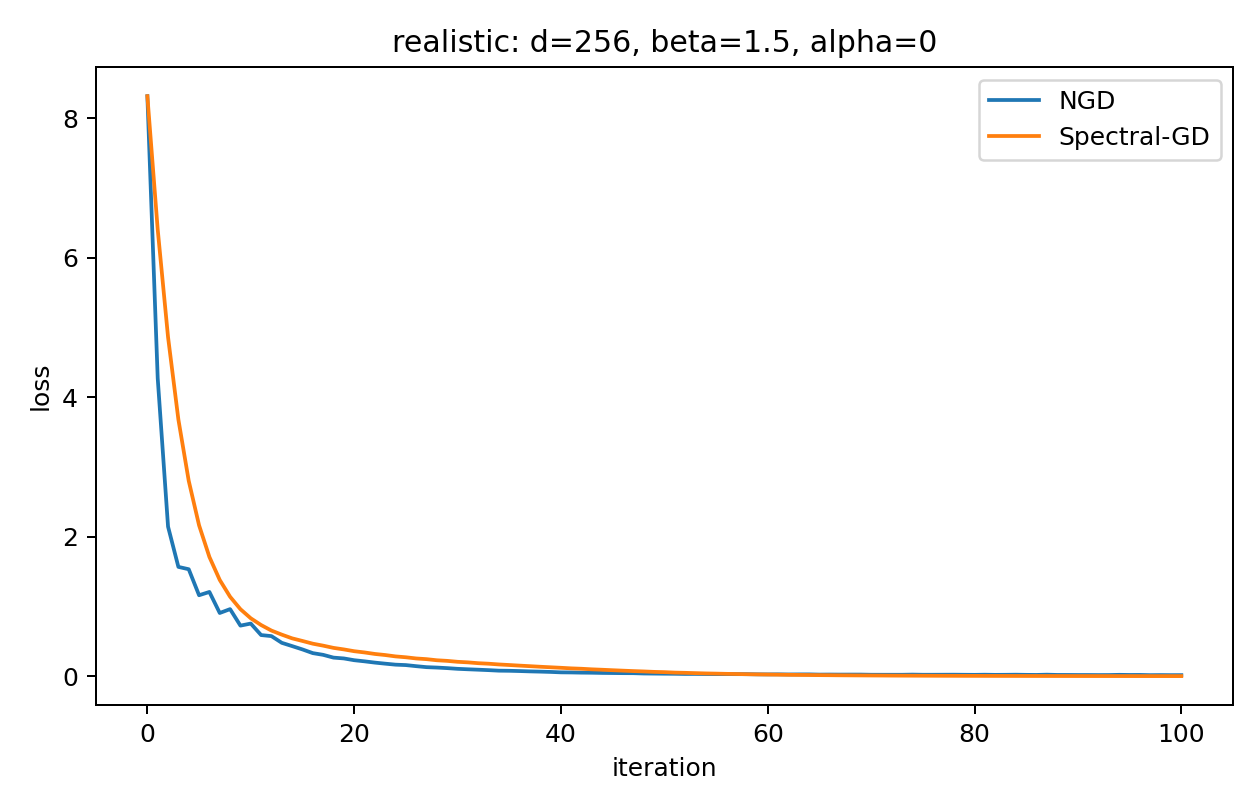
\includegraphics[width=\linewidth]{figures/loss_curves/realistic_d256_b1.5_a0.png}
\caption{$\alpha=0$}
\end{subfigure}%
\hfill
\begin{subfigure}{0.22\textwidth}
\centering
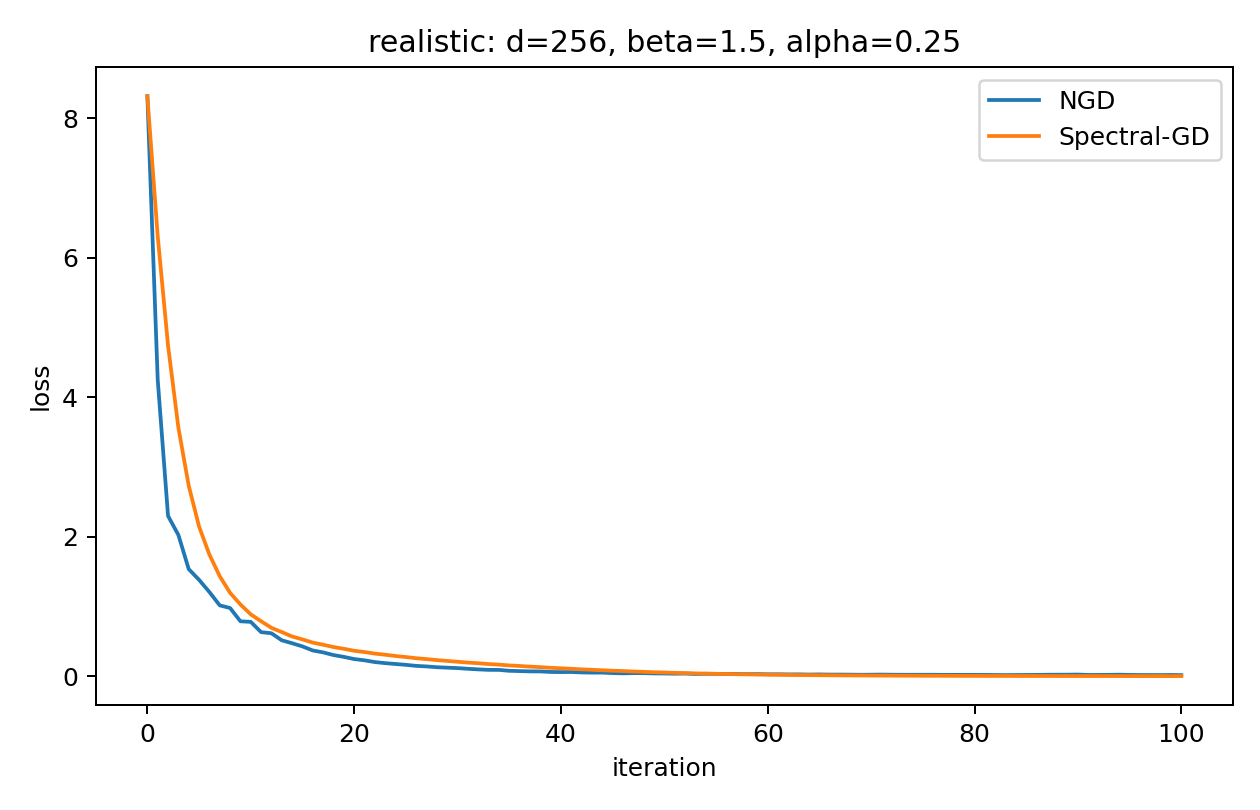
\includegraphics[width=\linewidth]{figures/loss_curves/realistic_d256_b1.5_a0.25.png}
\caption{$\alpha=0.25$}
\end{subfigure}%
\hfill
\begin{subfigure}{0.22\textwidth}
\centering
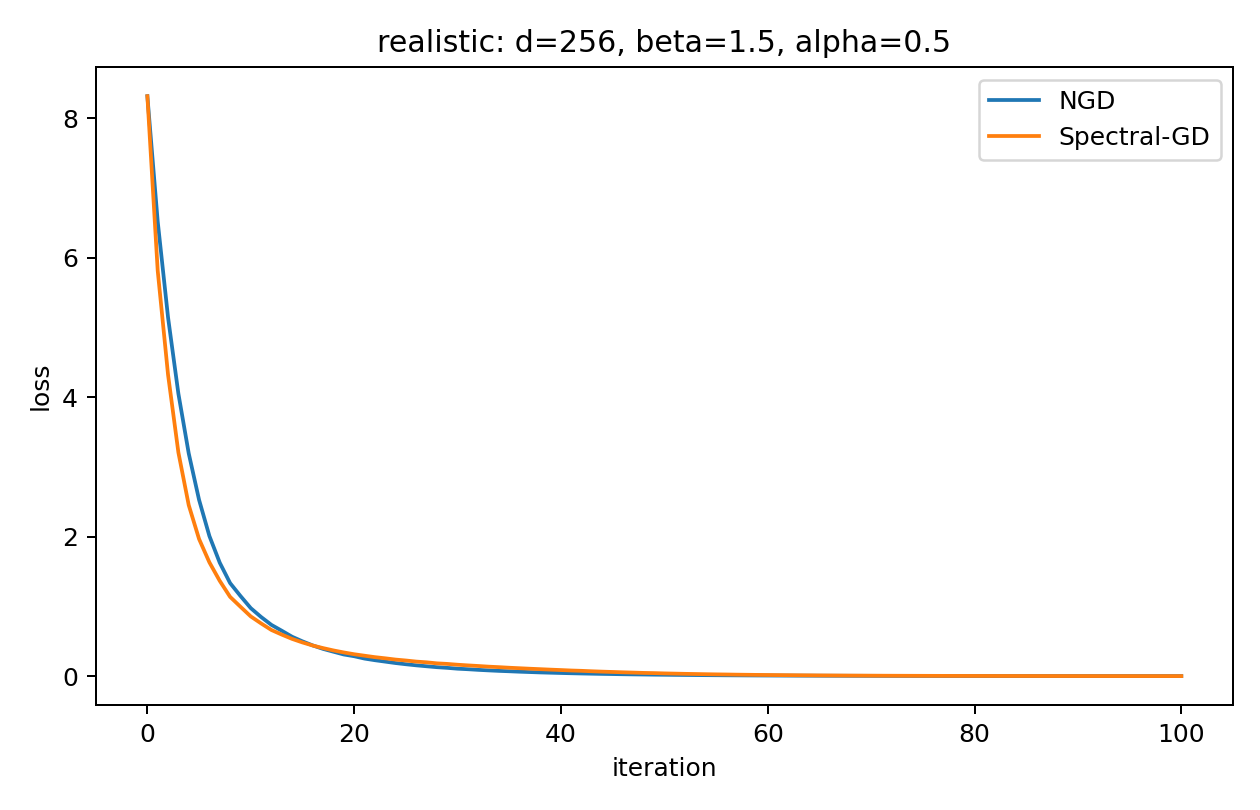
\includegraphics[width=\linewidth]{figures/loss_curves/realistic_d256_b1.5_a0.5.png}
\caption{$\alpha=0.5$}
\end{subfigure}%
\hfill
\begin{subfigure}{0.22\textwidth}
\centering
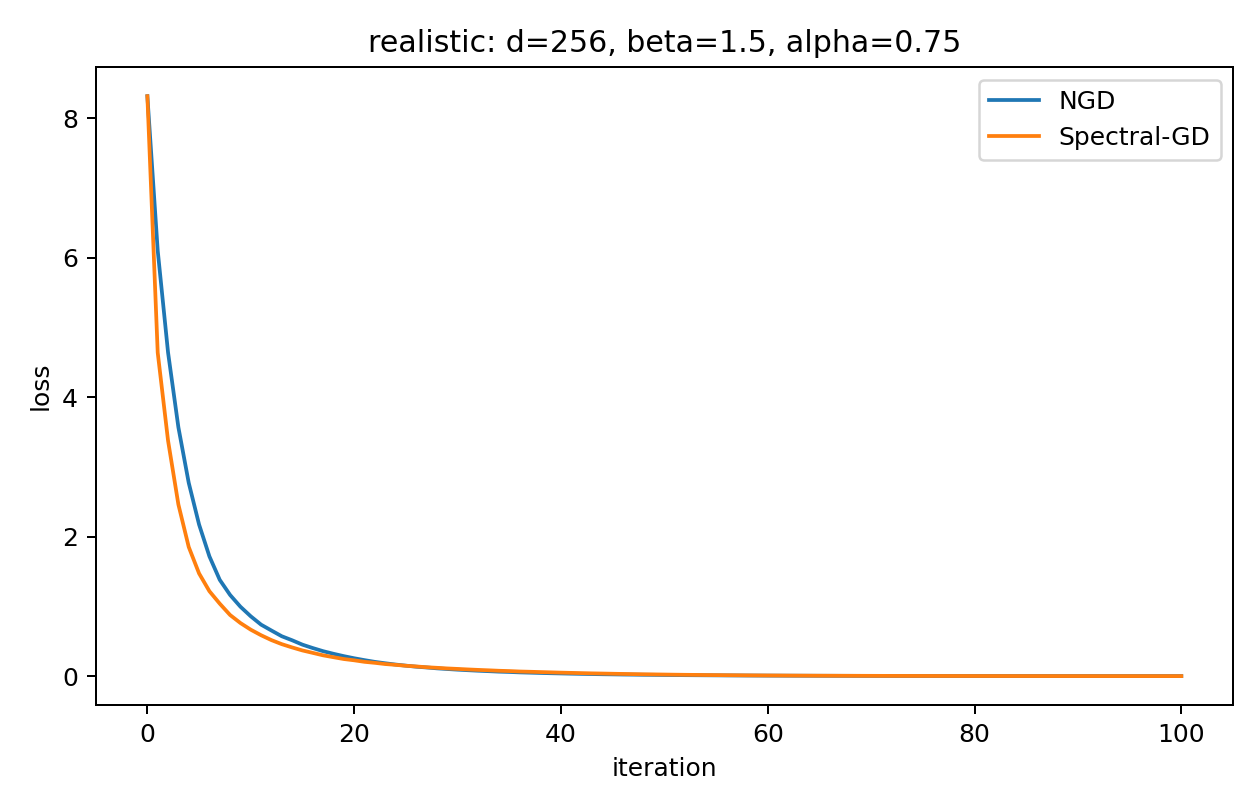
\includegraphics[width=\linewidth]{figures/loss_curves/realistic_d256_b1.5_a0.75.png}
\caption{$\alpha=0.75$}
\end{subfigure}%
\par\smallskip
\begin{subfigure}{0.22\textwidth}
\centering
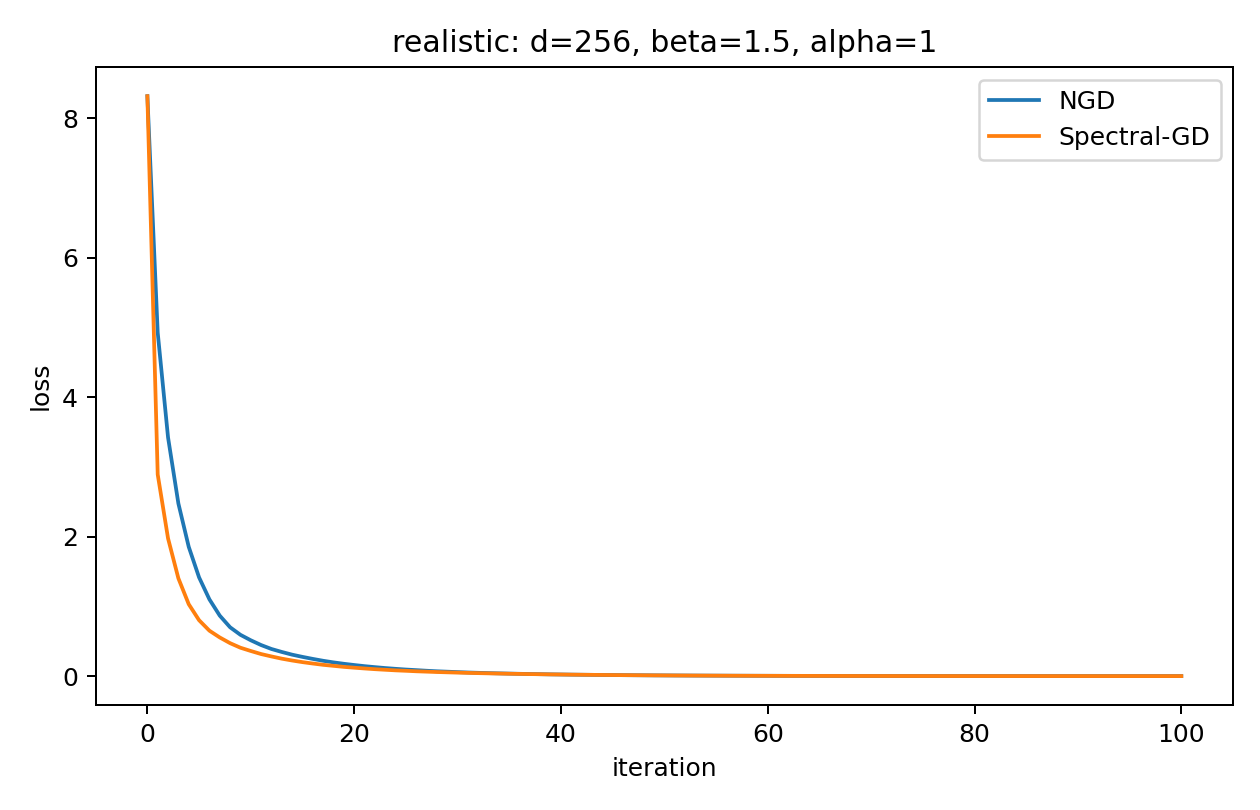
\includegraphics[width=\linewidth]{figures/loss_curves/realistic_d256_b1.5_a1.png}
\caption{$\alpha=1$}
\end{subfigure}%
\hfill
\begin{subfigure}{0.22\textwidth}
\centering
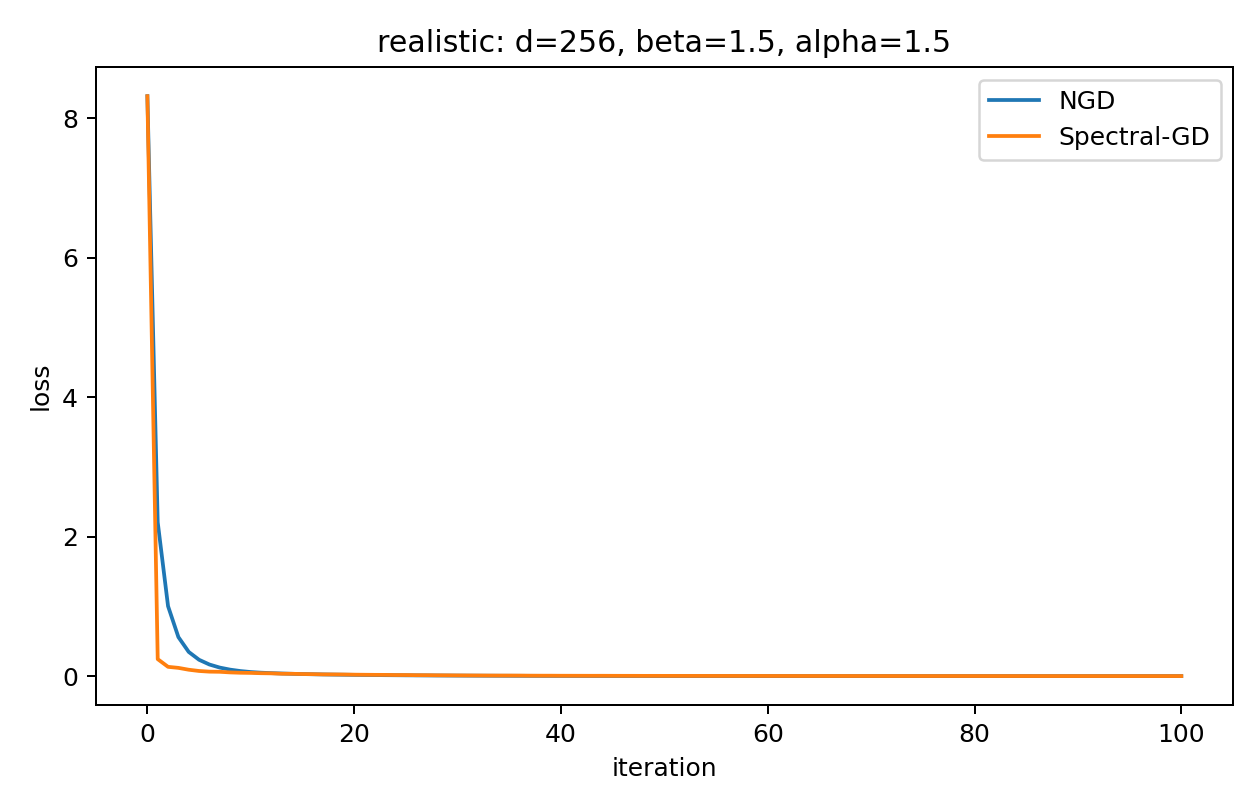
\includegraphics[width=\linewidth]{figures/loss_curves/realistic_d256_b1.5_a1.5.png}
\caption{$\alpha=1.5$}
\end{subfigure}%
\hfill
\begin{subfigure}{0.22\textwidth}
\centering
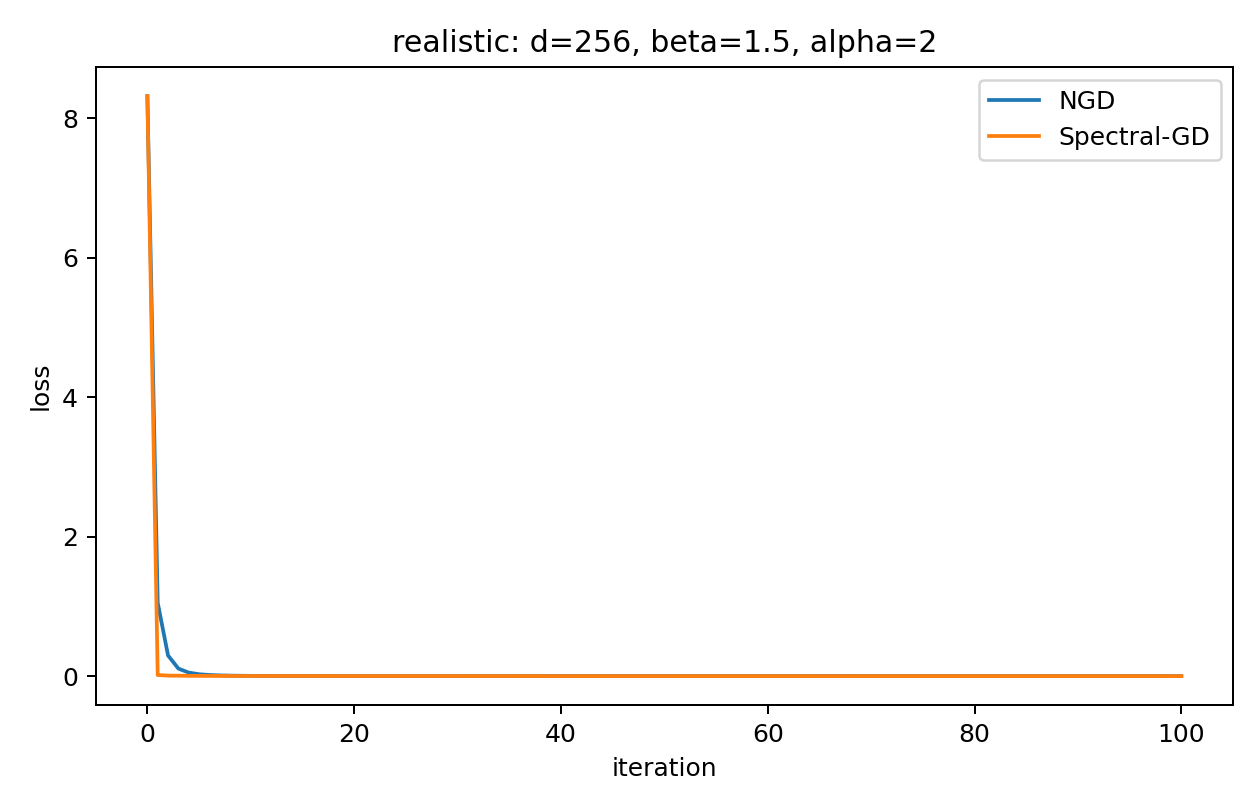
\includegraphics[width=\linewidth]{figures/loss_curves/realistic_d256_b1.5_a2.png}
\caption{$\alpha=2$}
\end{subfigure}%
\caption{Best-auc loss curves for realistic training, $\beta=1.5$, $d=256$, $N=4096$. Each panel is one value of $\alpha$. The solid line is the seed median and the shaded band is the interquartile range over three seeds.}
\label{fig:realistic:loss:b15}
\end{figure}


\begin{figure}[H]
\centering
\begin{subfigure}{0.22\textwidth}
\centering

\includegraphics[width=\linewidth]{figures/loss_envelope_curves/realistic_d256_b1.5_a0.png}
\caption{$\alpha=0$}
\end{subfigure}%
\hfill
\begin{subfigure}{0.22\textwidth}
\centering

\includegraphics[width=\linewidth]{figures/loss_envelope_curves/realistic_d256_b1.5_a0.25.png}
\caption{$\alpha=0.25$}
\end{subfigure}%
\hfill
\begin{subfigure}{0.22\textwidth}
\centering

\includegraphics[width=\linewidth]{figures/loss_envelope_curves/realistic_d256_b1.5_a0.5.png}
\caption{$\alpha=0.5$}
\end{subfigure}%
\hfill
\begin{subfigure}{0.22\textwidth}
\centering

\includegraphics[width=\linewidth]{figures/loss_envelope_curves/realistic_d256_b1.5_a0.75.png}
\caption{$\alpha=0.75$}
\end{subfigure}%
\par\smallskip
\begin{subfigure}{0.22\textwidth}
\centering

\includegraphics[width=\linewidth]{figures/loss_envelope_curves/realistic_d256_b1.5_a1.png}
\caption{$\alpha=1$}
\end{subfigure}%
\hfill
\begin{subfigure}{0.22\textwidth}
\centering

\includegraphics[width=\linewidth]{figures/loss_envelope_curves/realistic_d256_b1.5_a1.5.png}
\caption{$\alpha=1.5$}
\end{subfigure}%
\hfill
\begin{subfigure}{0.22\textwidth}
\centering

\includegraphics[width=\linewidth]{figures/loss_envelope_curves/realistic_d256_b1.5_a2.png}
\caption{$\alpha=2$}
\end{subfigure}%
\caption{Loss envelope curves for realistic training, $\beta=1.5$, $d=256$, $N=4096$. Each panel is one value of $\alpha$. The solid line is the seed median and the shaded band is the interquartile range over three seeds.}
\label{fig:realistic:envelope:b15}
\end{figure}


\begin{figure}[H]
\centering
\begin{subfigure}{0.22\textwidth}
\centering
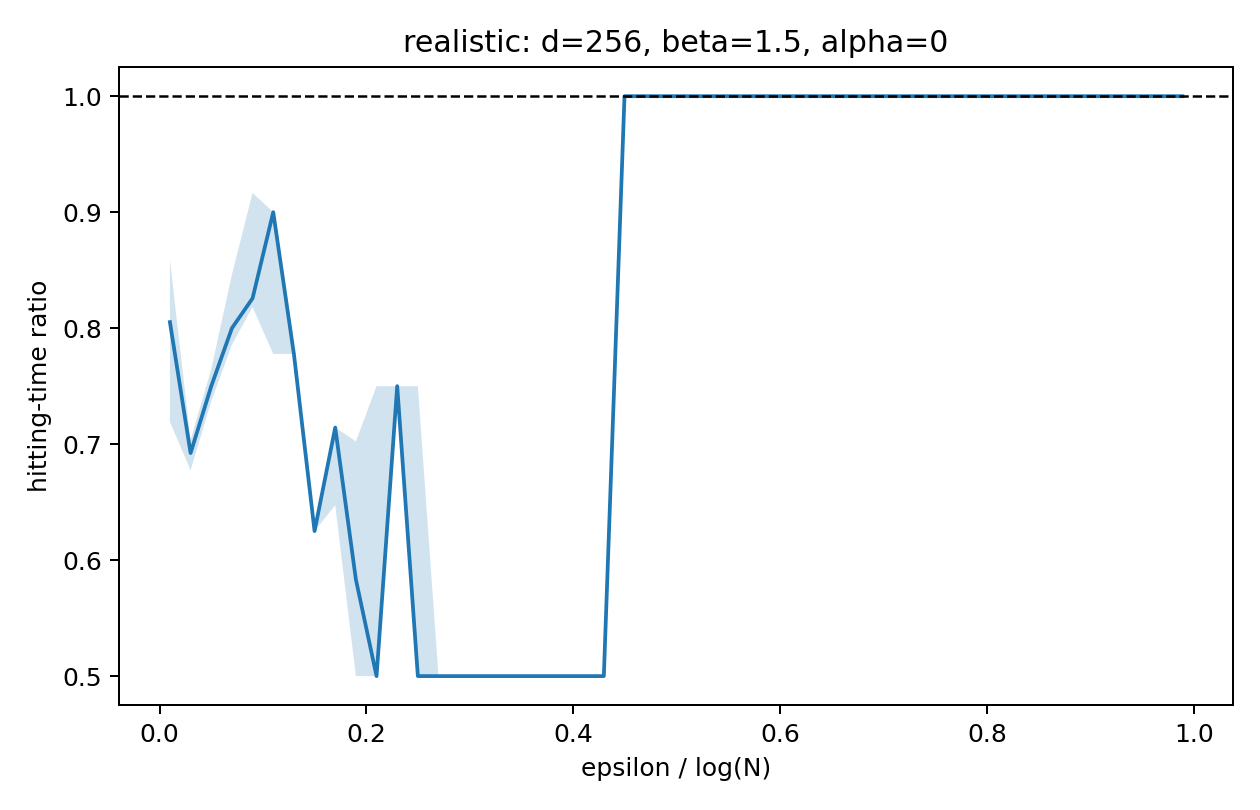
\includegraphics[width=\linewidth]{figures/ratio_curves/T_ratio_realistic_d256_b1.5_a0.png}
\caption{$\alpha=0$}
\end{subfigure}%
\hfill
\begin{subfigure}{0.22\textwidth}
\centering
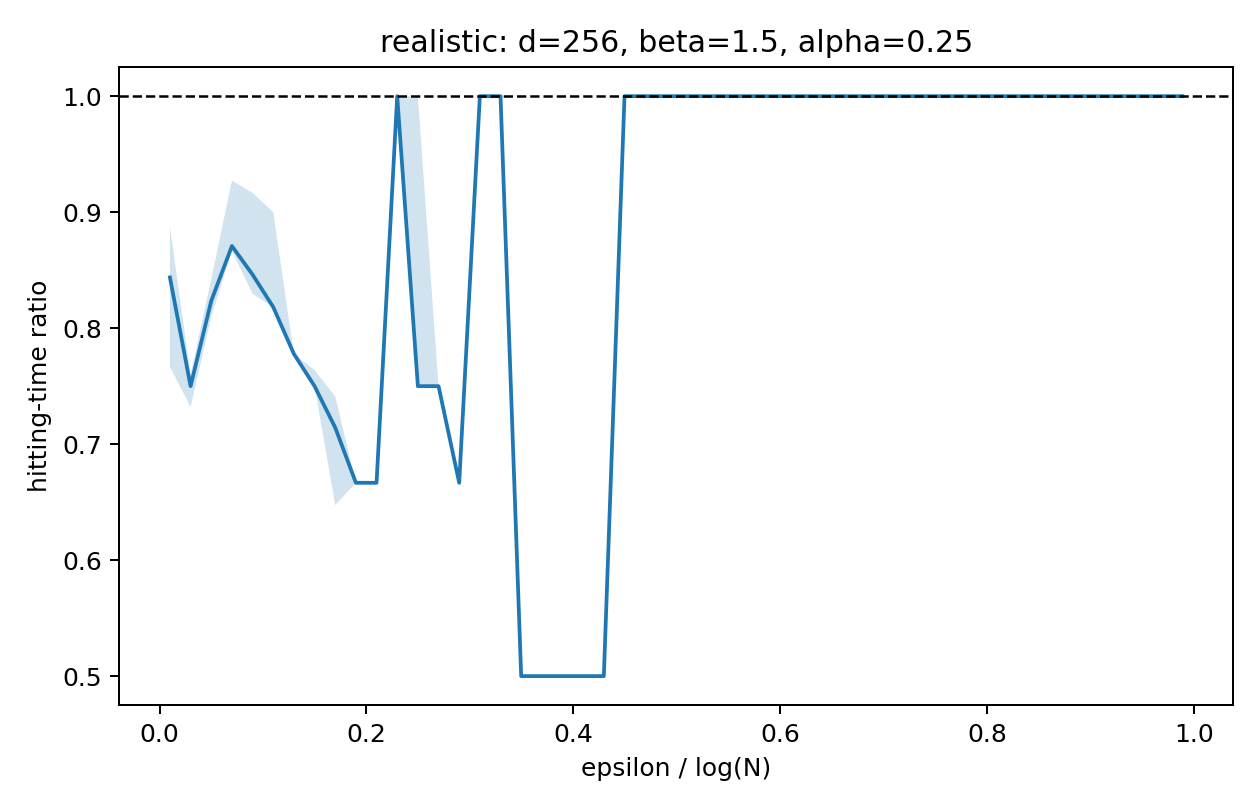
\includegraphics[width=\linewidth]{figures/ratio_curves/T_ratio_realistic_d256_b1.5_a0.25.png}
\caption{$\alpha=0.25$}
\end{subfigure}%
\hfill
\begin{subfigure}{0.22\textwidth}
\centering
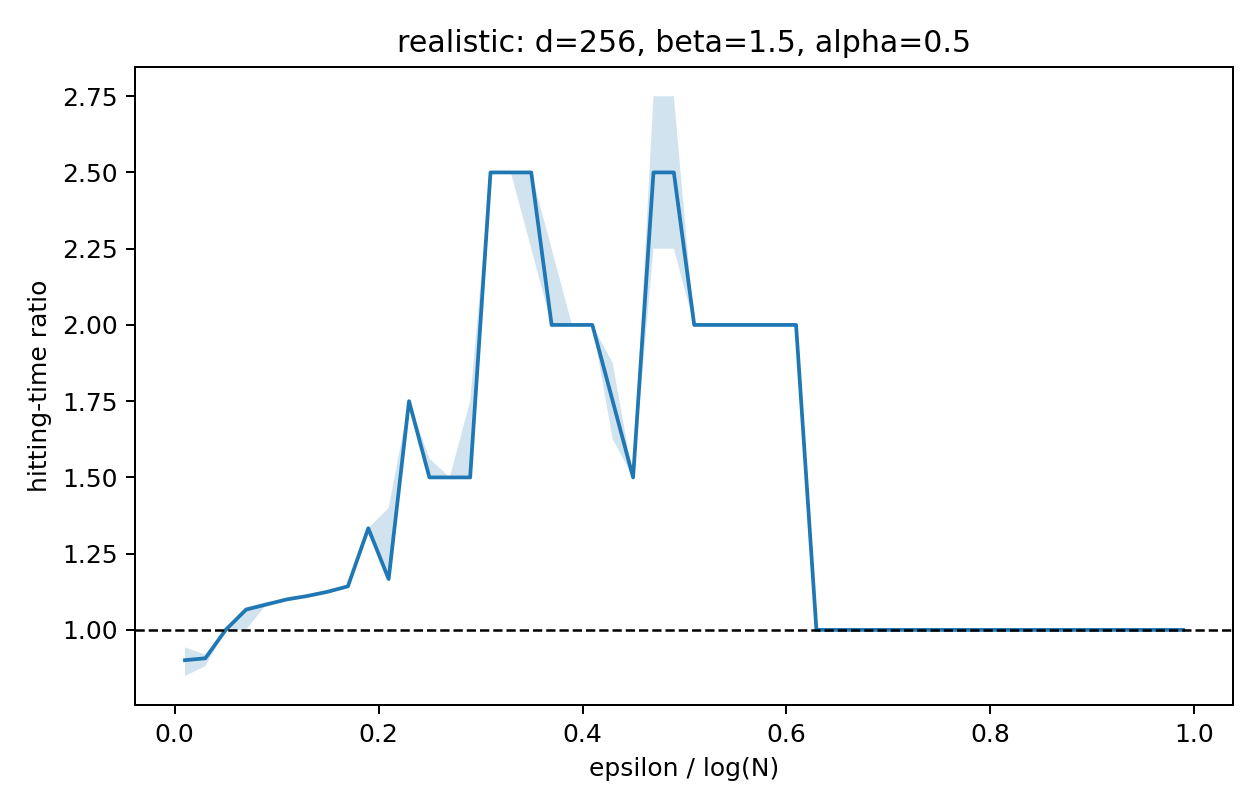
\includegraphics[width=\linewidth]{figures/ratio_curves/T_ratio_realistic_d256_b1.5_a0.5.png}
\caption{$\alpha=0.5$}
\end{subfigure}%
\hfill
\begin{subfigure}{0.22\textwidth}
\centering
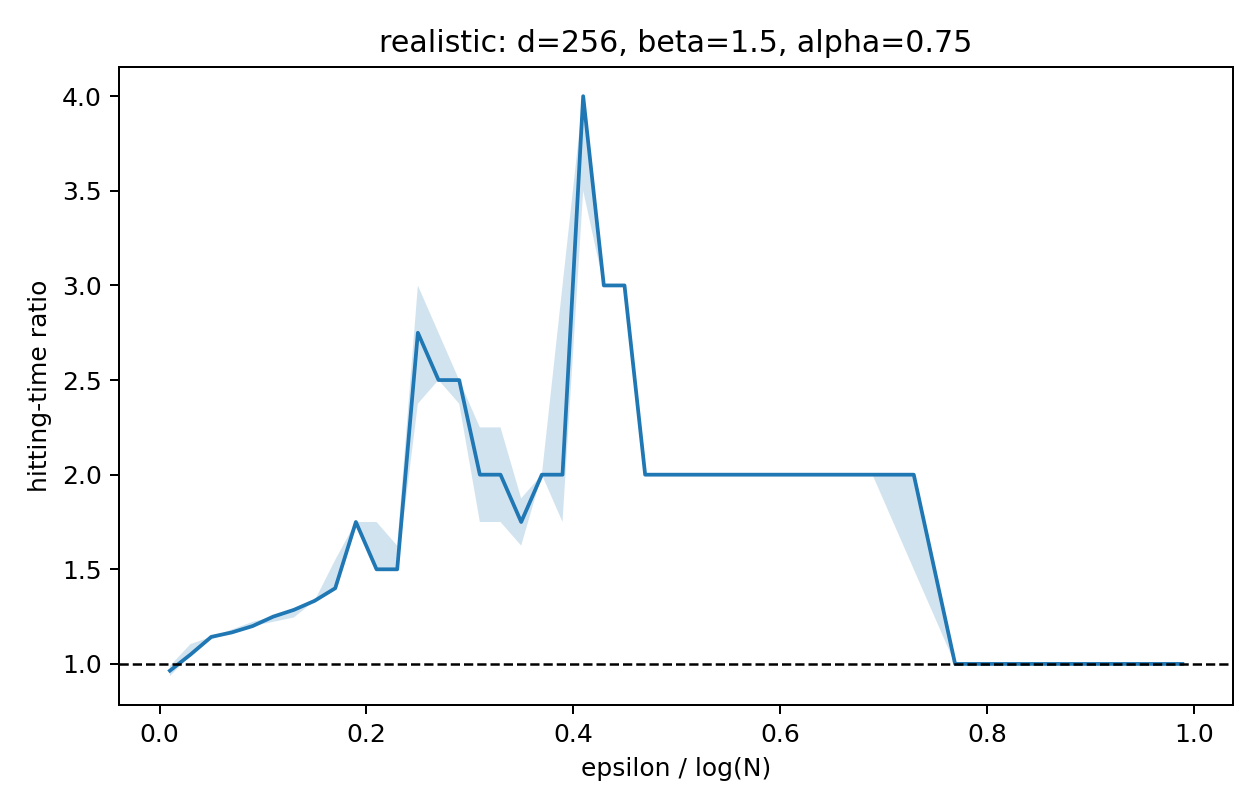
\includegraphics[width=\linewidth]{figures/ratio_curves/T_ratio_realistic_d256_b1.5_a0.75.png}
\caption{$\alpha=0.75$}
\end{subfigure}%
\par\smallskip
\begin{subfigure}{0.22\textwidth}
\centering
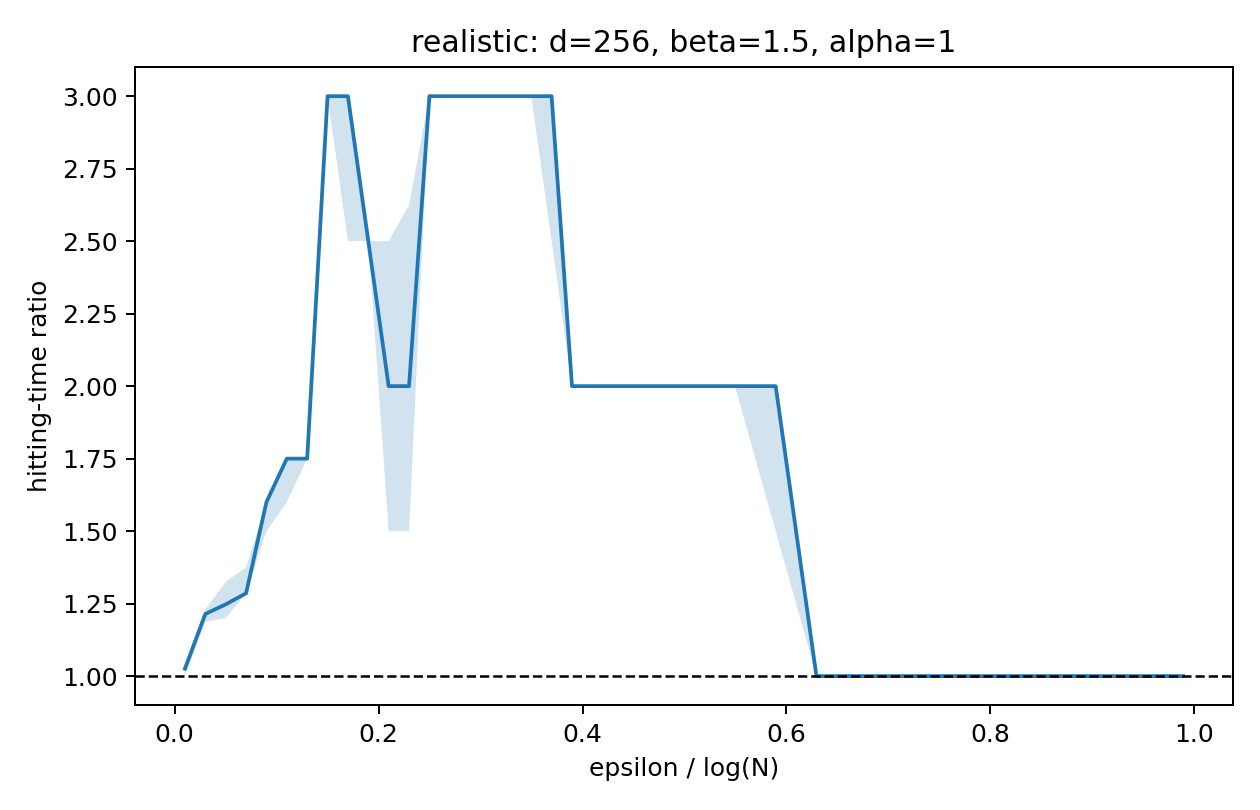
\includegraphics[width=\linewidth]{figures/ratio_curves/T_ratio_realistic_d256_b1.5_a1.png}
\caption{$\alpha=1$}
\end{subfigure}%
\hfill
\begin{subfigure}{0.22\textwidth}
\centering
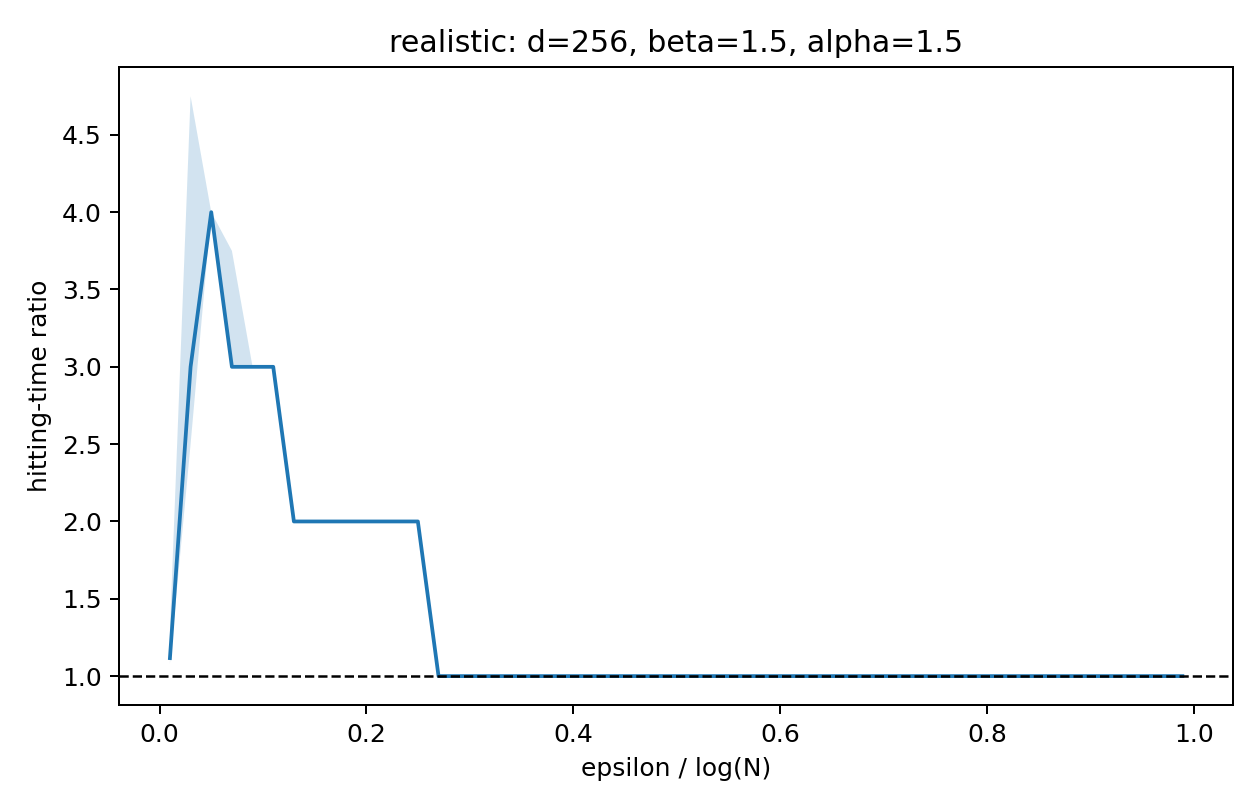
\includegraphics[width=\linewidth]{figures/ratio_curves/T_ratio_realistic_d256_b1.5_a1.5.png}
\caption{$\alpha=1.5$}
\end{subfigure}%
\hfill
\begin{subfigure}{0.22\textwidth}
\centering
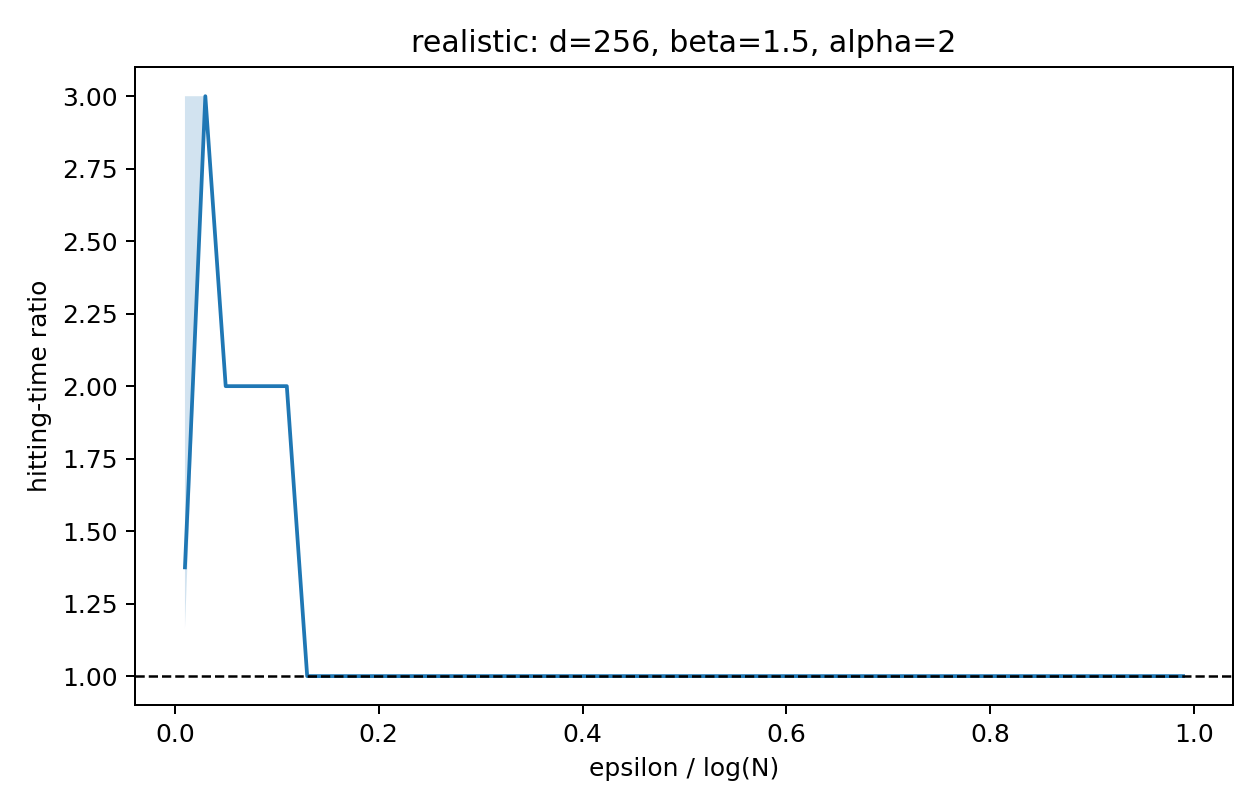
\includegraphics[width=\linewidth]{figures/ratio_curves/T_ratio_realistic_d256_b1.5_a2.png}
\caption{$\alpha=2$}
\end{subfigure}%
\caption{Hitting-time ratio curves for realistic training, $\beta=1.5$, $d=256$, $N=4096$. Each panel is one value of $\alpha$. The solid line is the seed median and the shaded band is the interquartile range over three seeds.}
\label{fig:realistic:T_ratio:b15}
\end{figure}






\subsubsection{$\beta_{\rm eff}=2.101845$, $d=80$, $N=10000$}

The following three figures show the complete alpha sweep for this beta block: the best-AUC loss traces, the per-step hyperparameter envelope, and the hitting-time ratio. Reading them together is important: the loss curves show ordinary tuned trajectories, the envelope shows the best loss achievable at each iteration under the sweep, and the hitting-time ratio is the primary speed metric.

\begin{figure}[H]
\centering
\begin{subfigure}{0.22\textwidth}
\centering
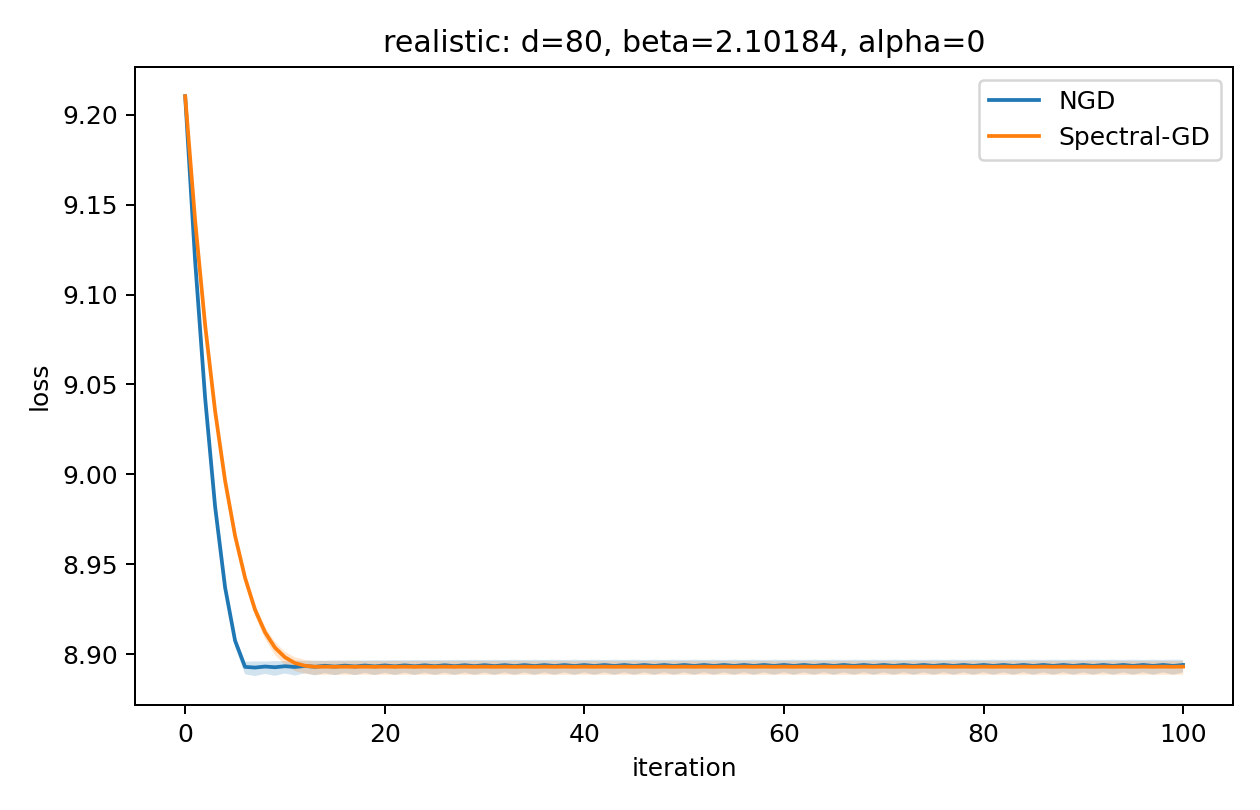
\includegraphics[width=\linewidth]{figures/loss_curves/realistic_d80_b2.10184_a0.png}
\caption{$\alpha=0$}
\end{subfigure}%
\hfill
\begin{subfigure}{0.22\textwidth}
\centering
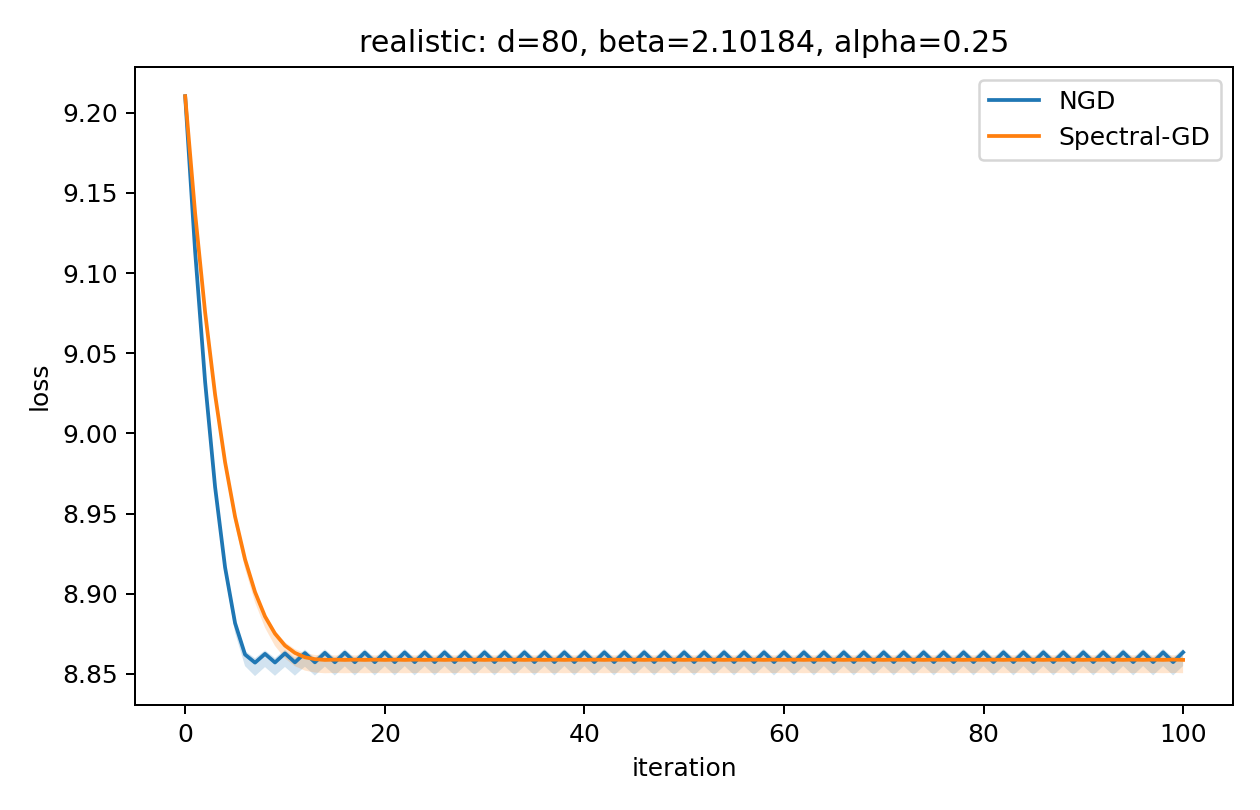
\includegraphics[width=\linewidth]{figures/loss_curves/realistic_d80_b2.10184_a0.25.png}
\caption{$\alpha=0.25$}
\end{subfigure}%
\hfill
\begin{subfigure}{0.22\textwidth}
\centering
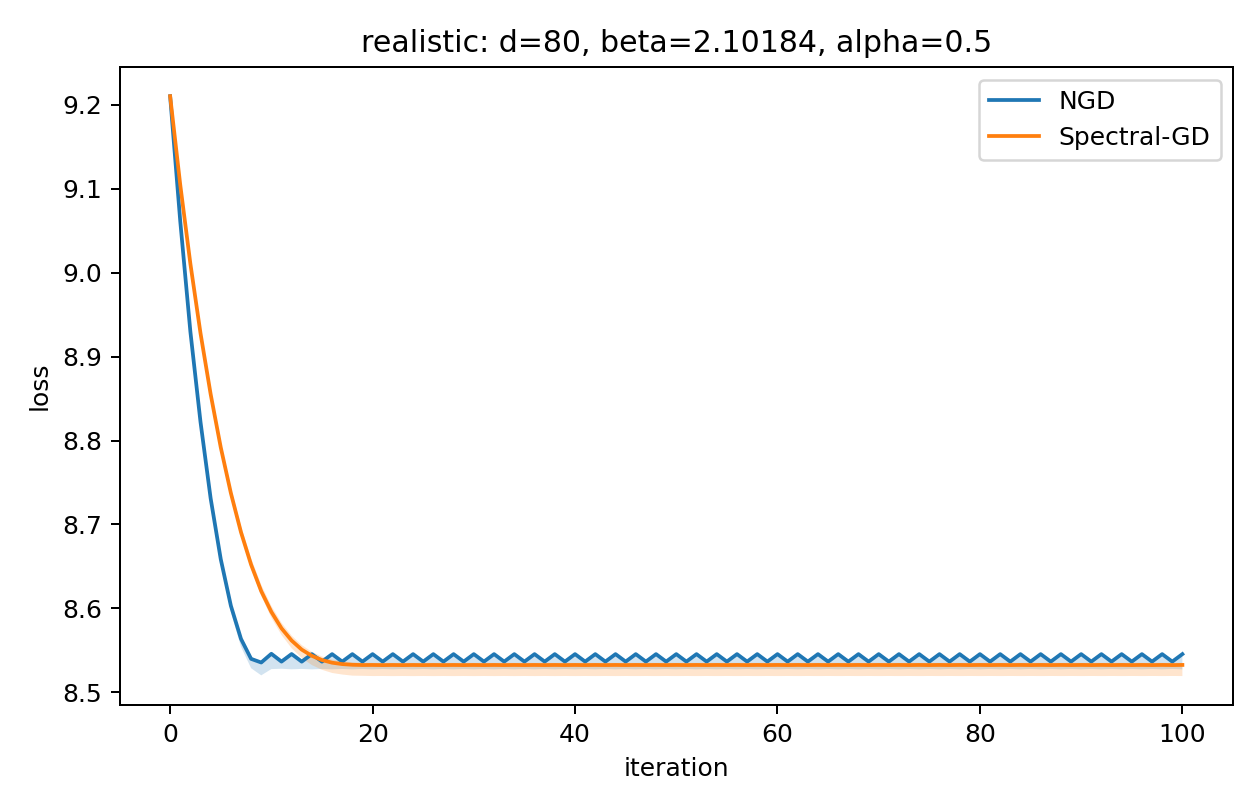
\includegraphics[width=\linewidth]{figures/loss_curves/realistic_d80_b2.10184_a0.5.png}
\caption{$\alpha=0.5$}
\end{subfigure}%
\hfill
\begin{subfigure}{0.22\textwidth}
\centering
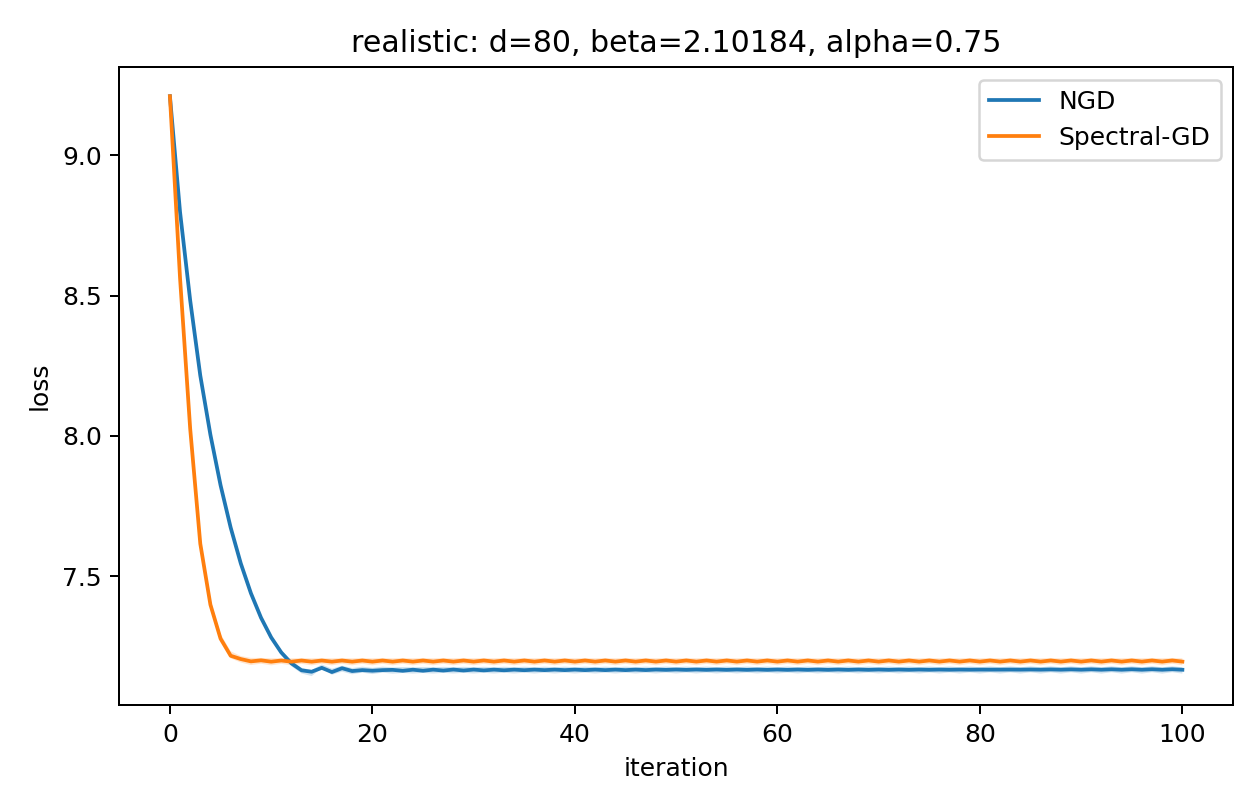
\includegraphics[width=\linewidth]{figures/loss_curves/realistic_d80_b2.10184_a0.75.png}
\caption{$\alpha=0.75$}
\end{subfigure}%
\par\smallskip
\begin{subfigure}{0.22\textwidth}
\centering
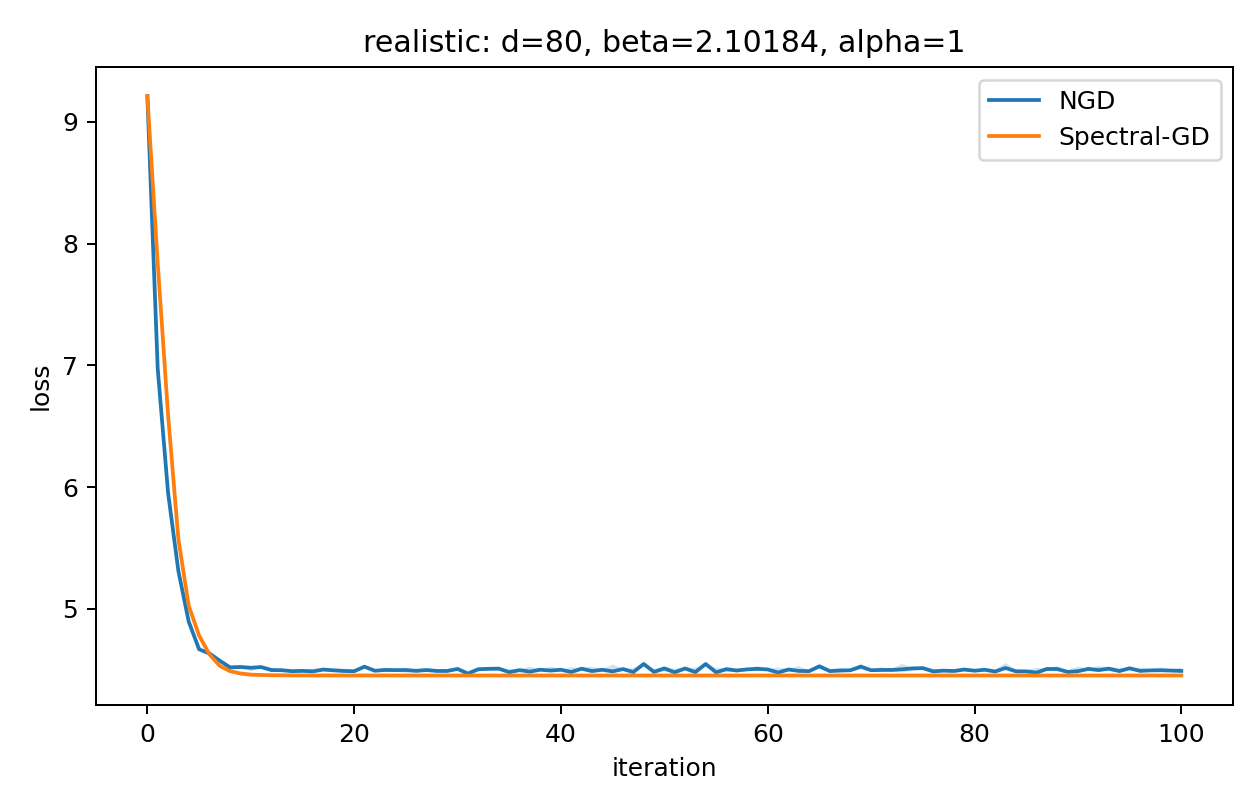
\includegraphics[width=\linewidth]{figures/loss_curves/realistic_d80_b2.10184_a1.png}
\caption{$\alpha=1$}
\end{subfigure}%
\hfill
\begin{subfigure}{0.22\textwidth}
\centering
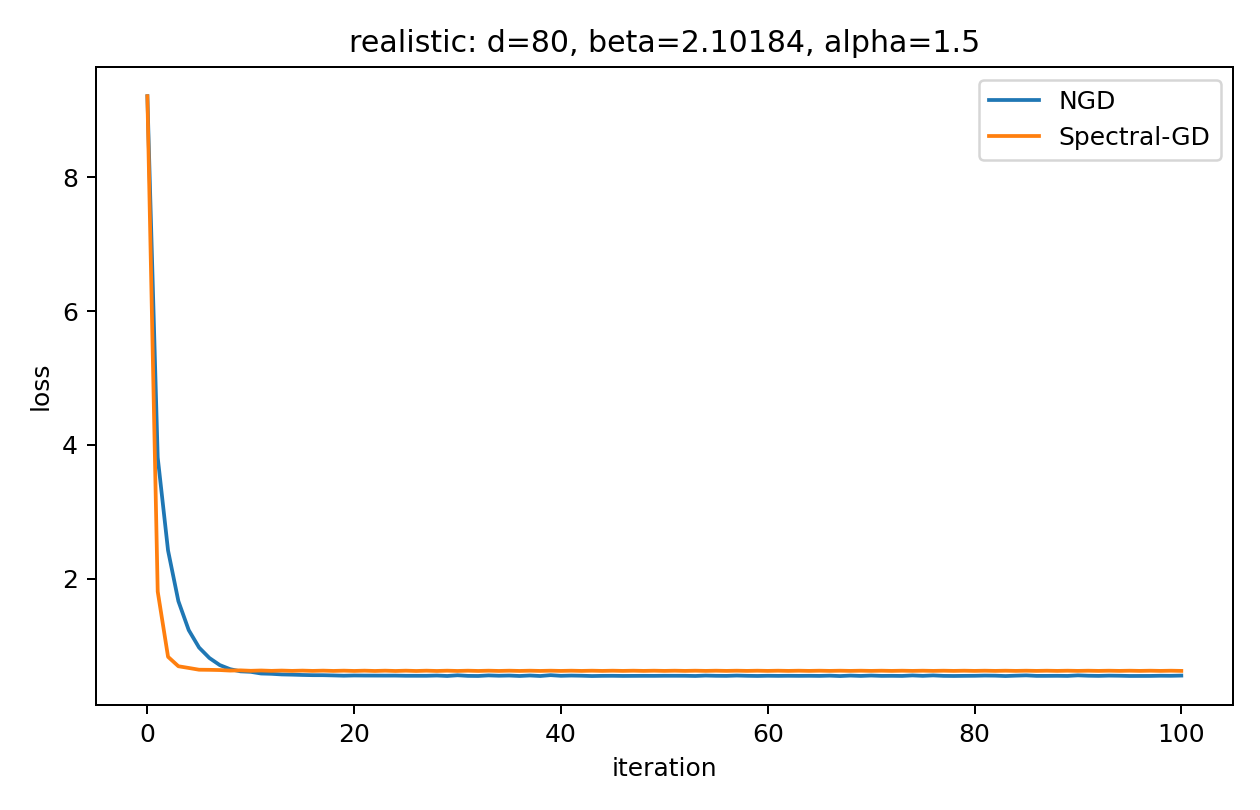
\includegraphics[width=\linewidth]{figures/loss_curves/realistic_d80_b2.10184_a1.5.png}
\caption{$\alpha=1.5$}
\end{subfigure}%
\hfill
\begin{subfigure}{0.22\textwidth}
\centering
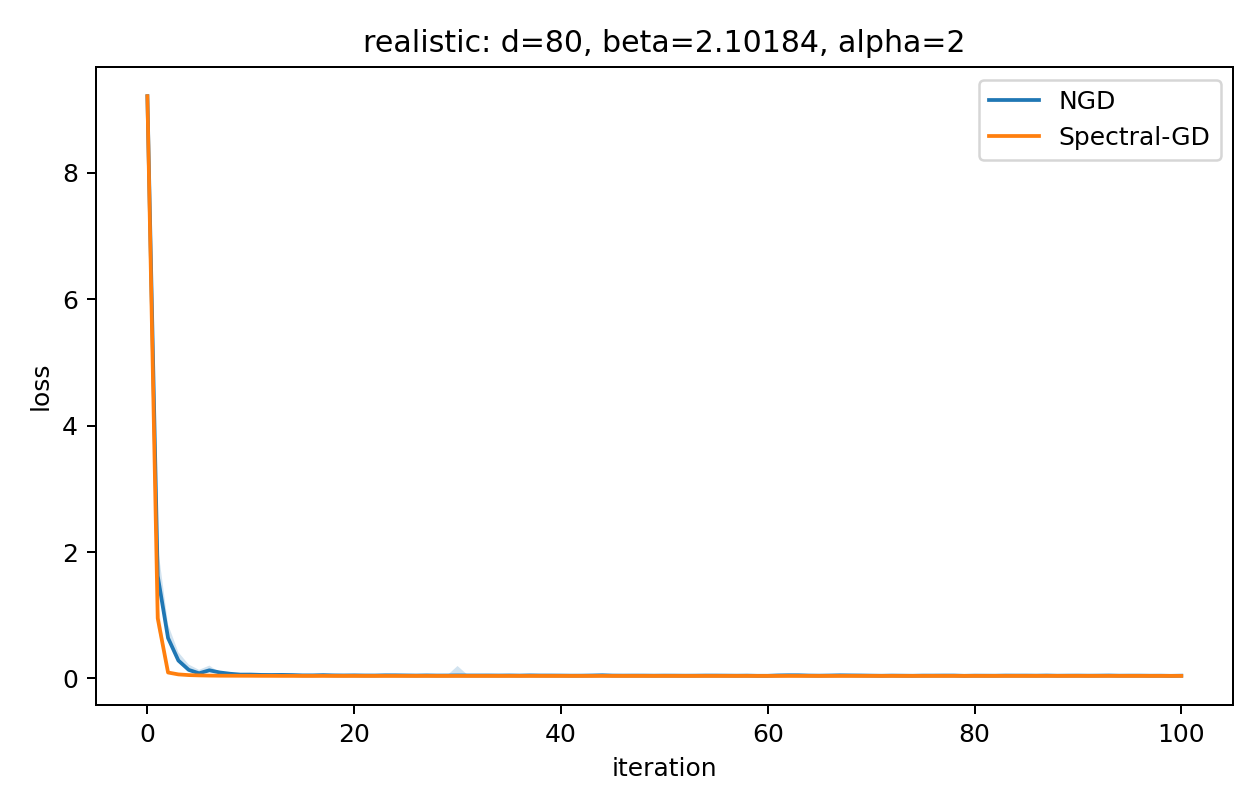
\includegraphics[width=\linewidth]{figures/loss_curves/realistic_d80_b2.10184_a2.png}
\caption{$\alpha=2$}
\end{subfigure}%
\caption{Best-auc loss curves for realistic training, $\beta_{\rm eff}=2.101845$, $d=80$, $N=10000$. Each panel is one value of $\alpha$. The solid line is the seed median and the shaded band is the interquartile range over three seeds.}
\label{fig:realistic:loss:beff210}
\end{figure}


\begin{figure}[H]
\centering
\begin{subfigure}{0.22\textwidth}
\centering

\includegraphics[width=\linewidth]{figures/loss_envelope_curves/realistic_d80_b2.10184_a0.png}
\caption{$\alpha=0$}
\end{subfigure}%
\hfill
\begin{subfigure}{0.22\textwidth}
\centering

\includegraphics[width=\linewidth]{figures/loss_envelope_curves/realistic_d80_b2.10184_a0.25.png}
\caption{$\alpha=0.25$}
\end{subfigure}%
\hfill
\begin{subfigure}{0.22\textwidth}
\centering

\includegraphics[width=\linewidth]{figures/loss_envelope_curves/realistic_d80_b2.10184_a0.5.png}
\caption{$\alpha=0.5$}
\end{subfigure}%
\hfill
\begin{subfigure}{0.22\textwidth}
\centering

\includegraphics[width=\linewidth]{figures/loss_envelope_curves/realistic_d80_b2.10184_a0.75.png}
\caption{$\alpha=0.75$}
\end{subfigure}%
\par\smallskip
\begin{subfigure}{0.22\textwidth}
\centering

\includegraphics[width=\linewidth]{figures/loss_envelope_curves/realistic_d80_b2.10184_a1.png}
\caption{$\alpha=1$}
\end{subfigure}%
\hfill
\begin{subfigure}{0.22\textwidth}
\centering

\includegraphics[width=\linewidth]{figures/loss_envelope_curves/realistic_d80_b2.10184_a1.5.png}
\caption{$\alpha=1.5$}
\end{subfigure}%
\hfill
\begin{subfigure}{0.22\textwidth}
\centering

\includegraphics[width=\linewidth]{figures/loss_envelope_curves/realistic_d80_b2.10184_a2.png}
\caption{$\alpha=2$}
\end{subfigure}%
\caption{Loss envelope curves for realistic training, $\beta_{\rm eff}=2.101845$, $d=80$, $N=10000$. Each panel is one value of $\alpha$. The solid line is the seed median and the shaded band is the interquartile range over three seeds.}
\label{fig:realistic:envelope:beff210}
\end{figure}


\begin{figure}[H]
\centering
\begin{subfigure}{0.22\textwidth}
\centering
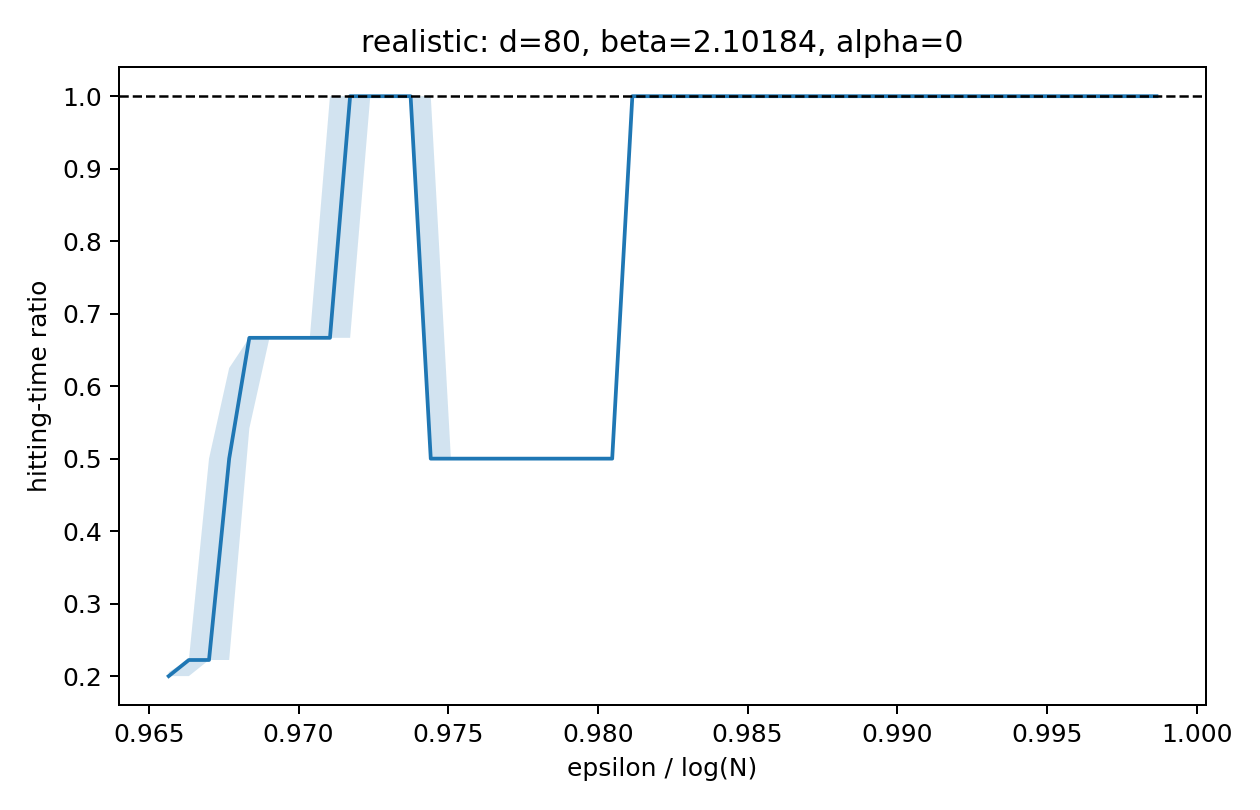
\includegraphics[width=\linewidth]{figures/ratio_curves/T_ratio_realistic_d80_b2.10184_a0.png}
\caption{$\alpha=0$}
\end{subfigure}%
\hfill
\begin{subfigure}{0.22\textwidth}
\centering
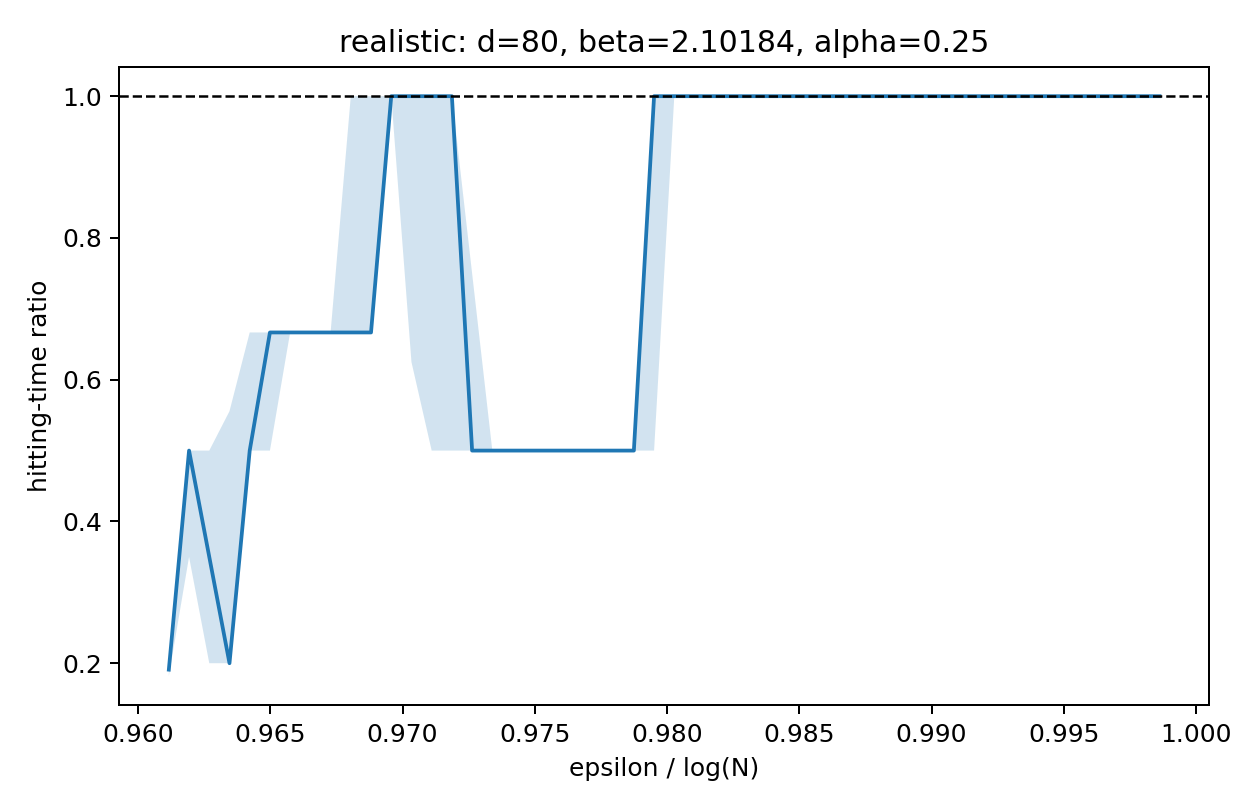
\includegraphics[width=\linewidth]{figures/ratio_curves/T_ratio_realistic_d80_b2.10184_a0.25.png}
\caption{$\alpha=0.25$}
\end{subfigure}%
\hfill
\begin{subfigure}{0.22\textwidth}
\centering
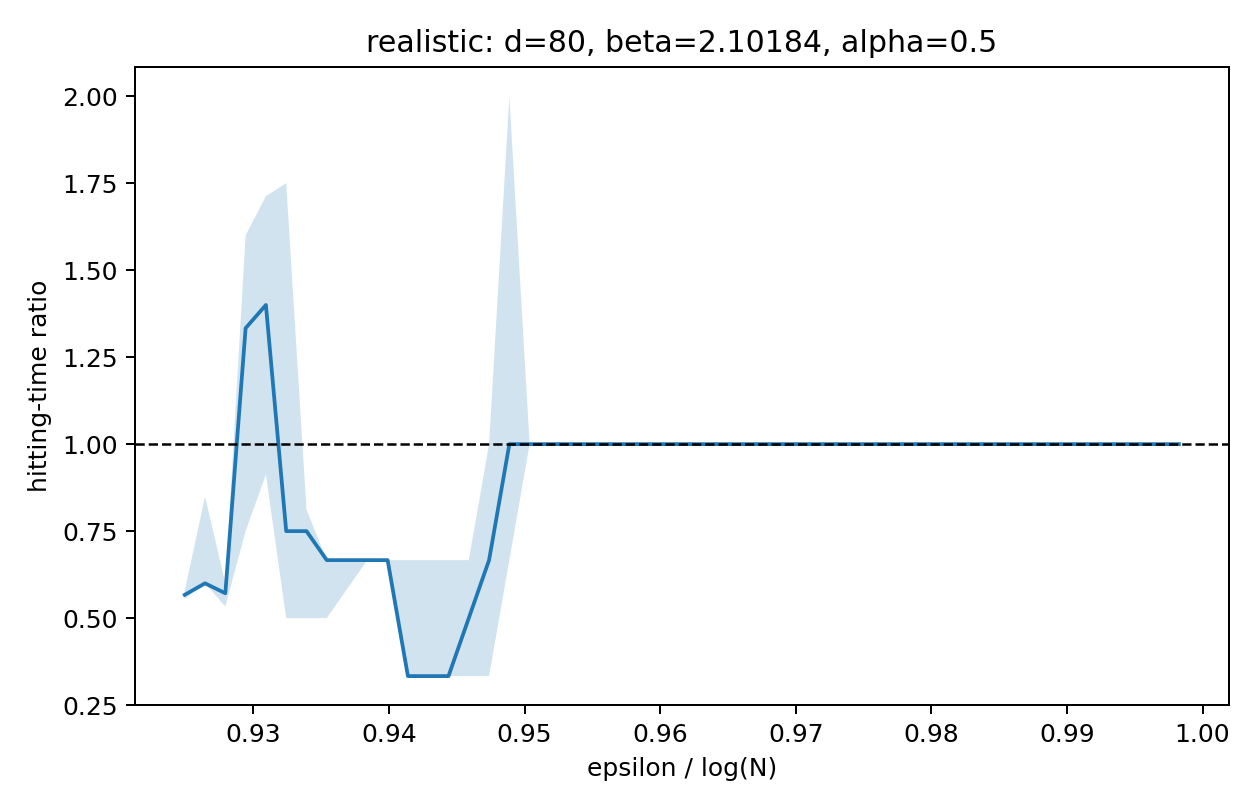
\includegraphics[width=\linewidth]{figures/ratio_curves/T_ratio_realistic_d80_b2.10184_a0.5.png}
\caption{$\alpha=0.5$}
\end{subfigure}%
\hfill
\begin{subfigure}{0.22\textwidth}
\centering
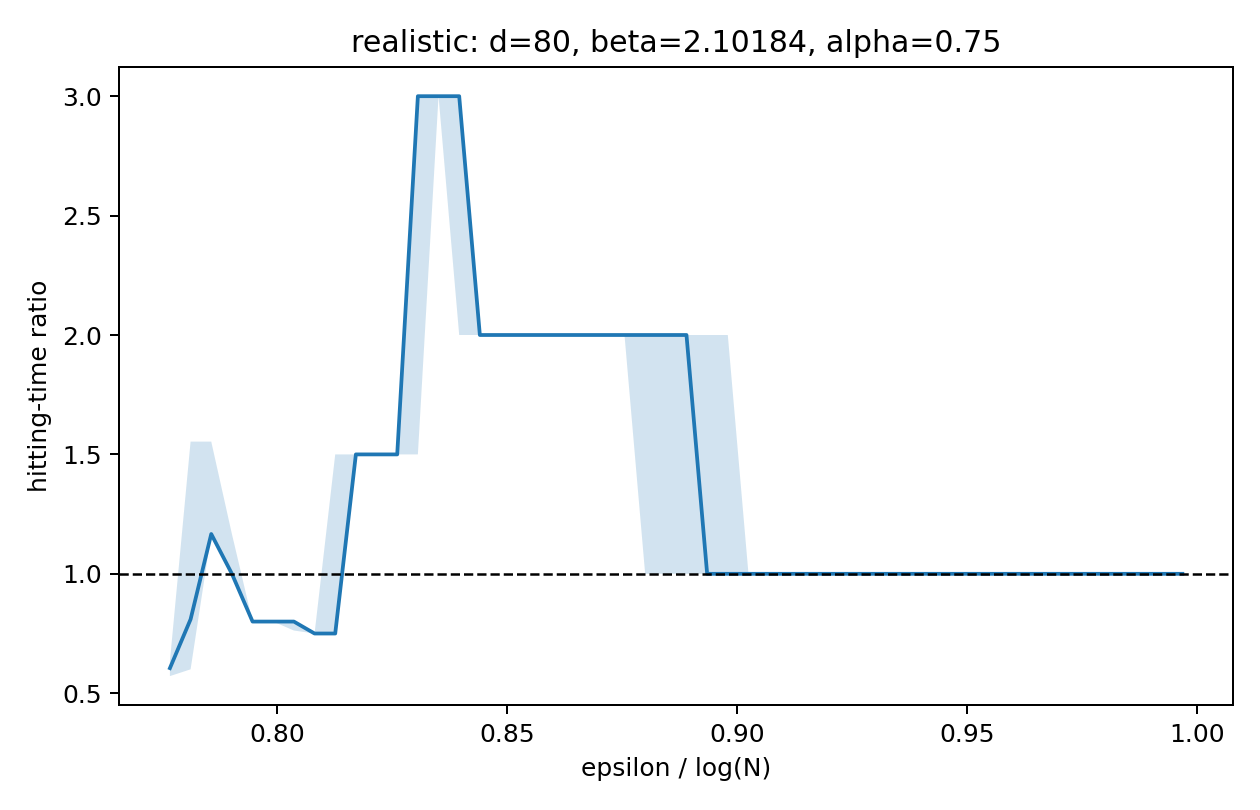
\includegraphics[width=\linewidth]{figures/ratio_curves/T_ratio_realistic_d80_b2.10184_a0.75.png}
\caption{$\alpha=0.75$}
\end{subfigure}%
\par\smallskip
\begin{subfigure}{0.22\textwidth}
\centering
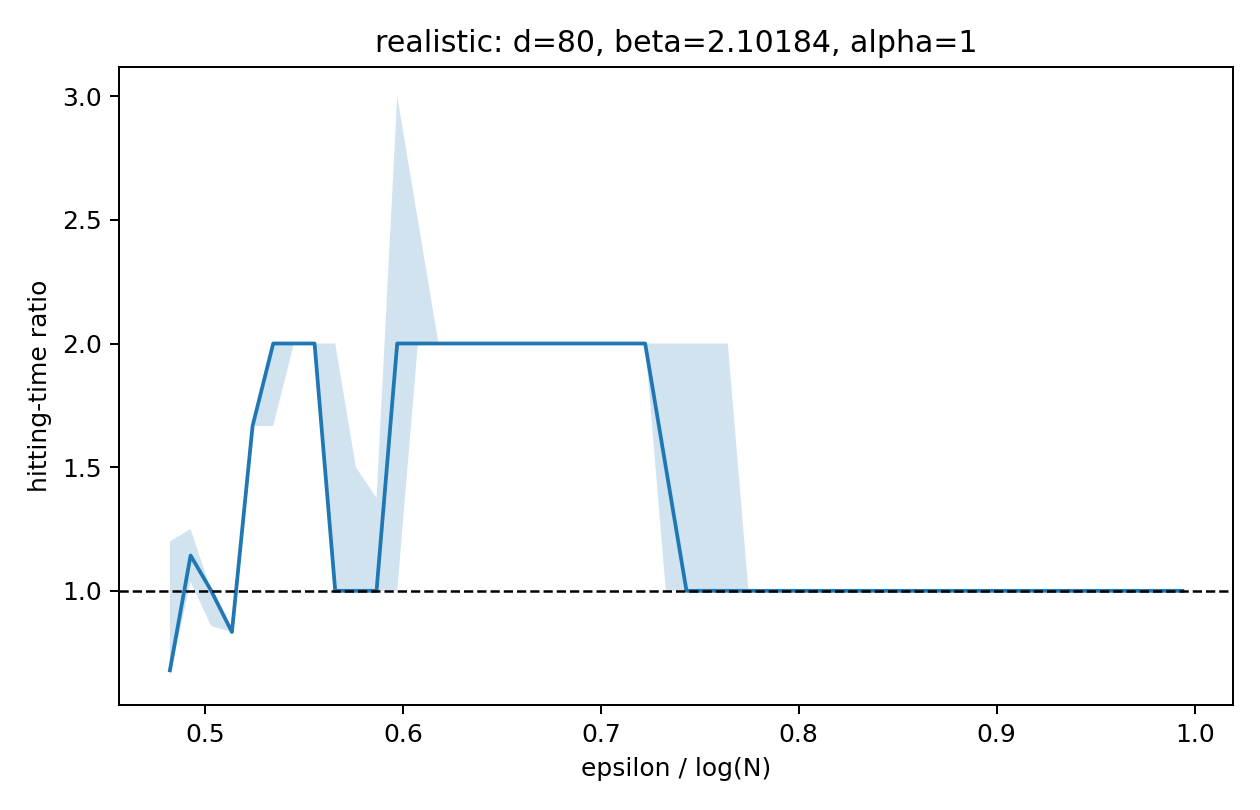
\includegraphics[width=\linewidth]{figures/ratio_curves/T_ratio_realistic_d80_b2.10184_a1.png}
\caption{$\alpha=1$}
\end{subfigure}%
\hfill
\begin{subfigure}{0.22\textwidth}
\centering
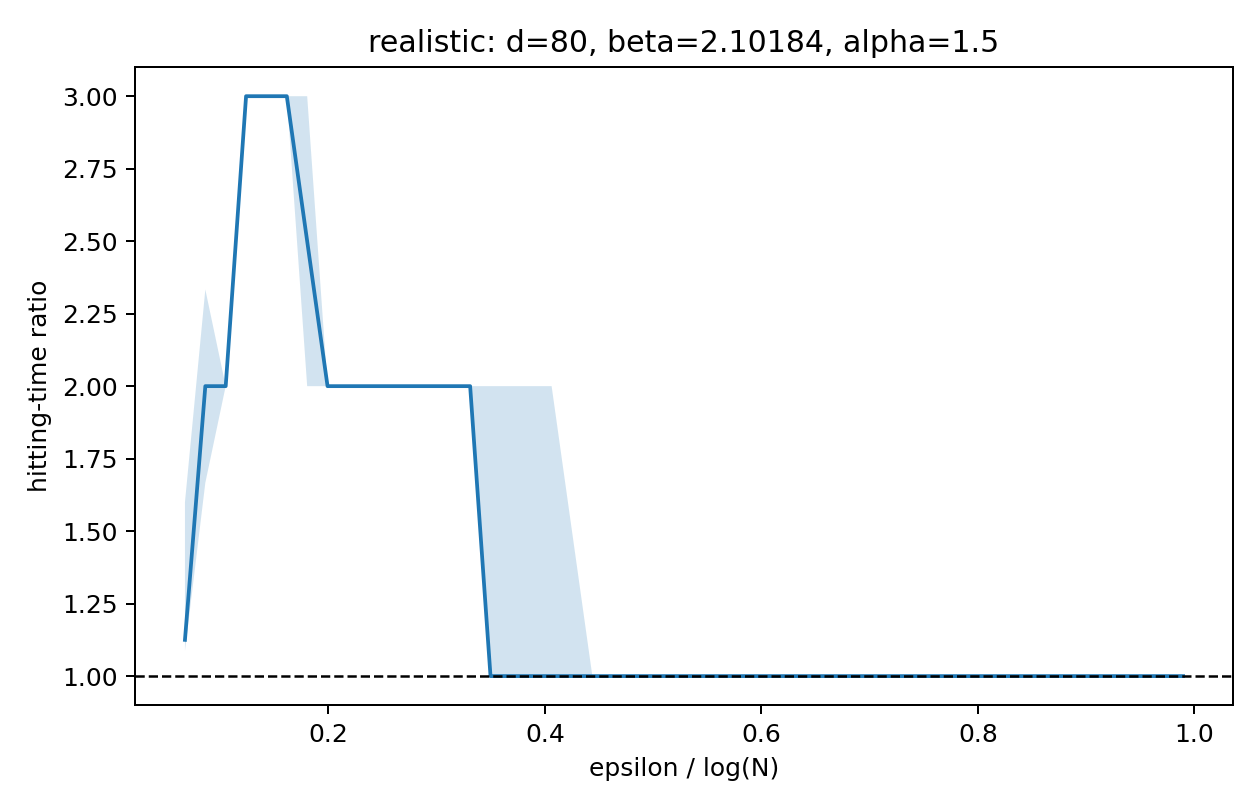
\includegraphics[width=\linewidth]{figures/ratio_curves/T_ratio_realistic_d80_b2.10184_a1.5.png}
\caption{$\alpha=1.5$}
\end{subfigure}%
\hfill
\begin{subfigure}{0.22\textwidth}
\centering
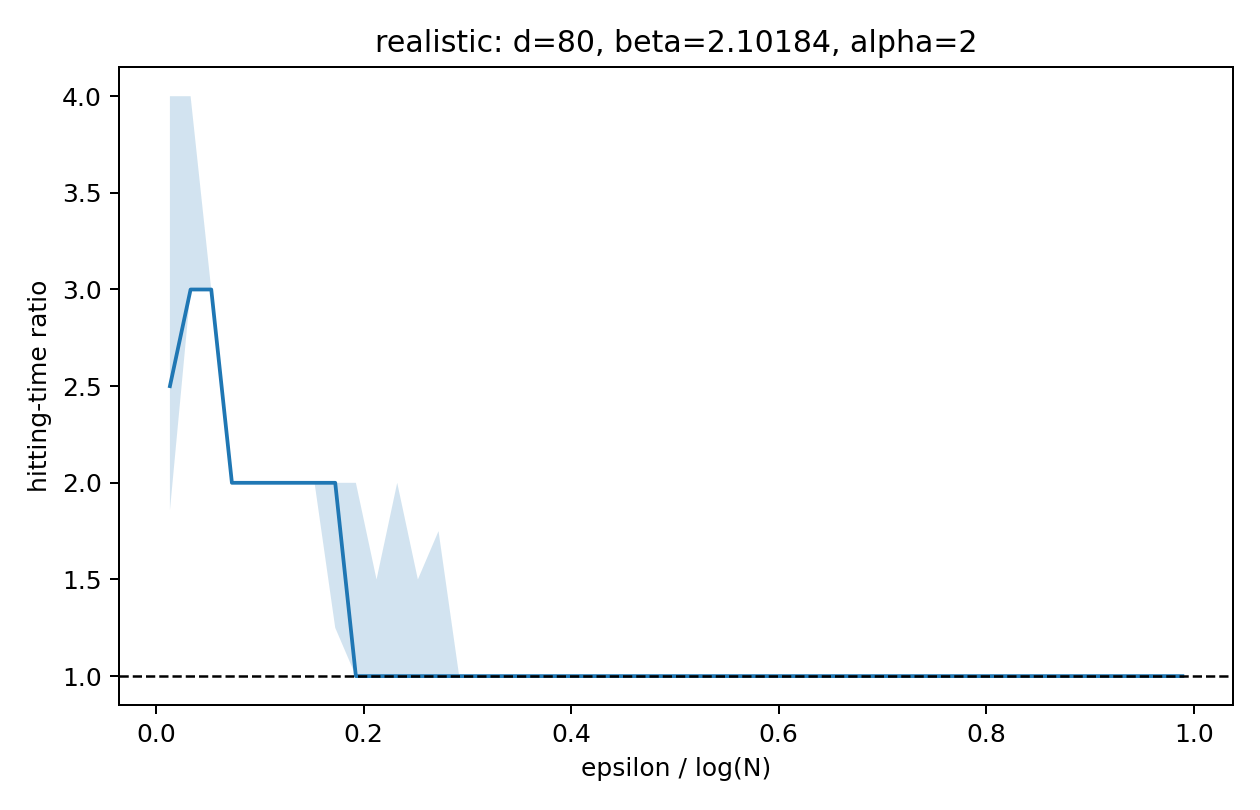
\includegraphics[width=\linewidth]{figures/ratio_curves/T_ratio_realistic_d80_b2.10184_a2.png}
\caption{$\alpha=2$}
\end{subfigure}%
\caption{Hitting-time ratio curves for realistic training, $\beta_{\rm eff}=2.101845$, $d=80$, $N=10000$. Each panel is one value of $\alpha$. The solid line is the seed median and the shaded band is the interquartile range over three seeds.}
\label{fig:realistic:T_ratio:beff210}
\end{figure}






\subsection{Complete alpha grids for Frank-Wolfe control}

\subsubsection{$\beta=0.75$, $d=256$, $N=64$}

The following three figures show the complete alpha sweep for this beta block: the best-AUC loss traces, the per-step hyperparameter envelope, and the hitting-time ratio. Reading them together is important: the loss curves show ordinary tuned trajectories, the envelope shows the best loss achievable at each iteration under the sweep, and the hitting-time ratio is the primary speed metric.

\begin{figure}[H]
\centering
\begin{subfigure}{0.22\textwidth}
\centering
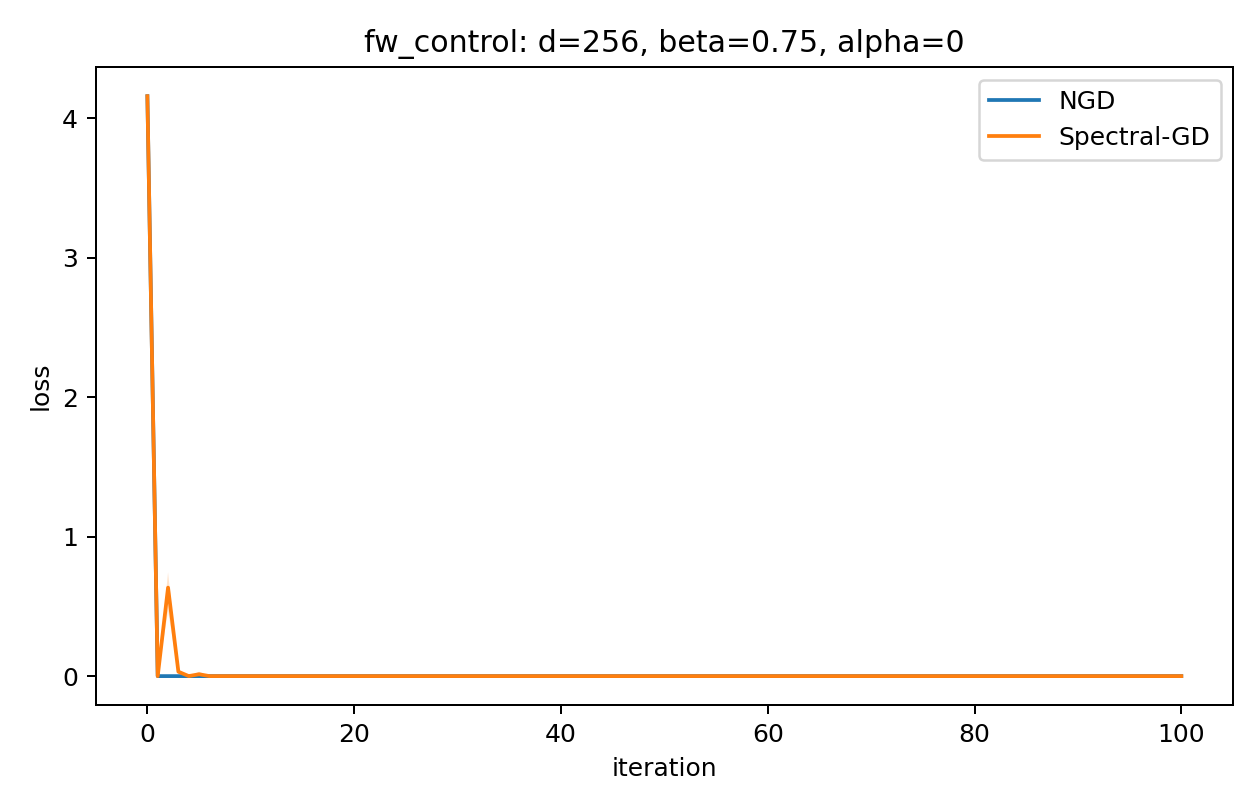
\includegraphics[width=\linewidth]{figures/loss_curves/fw_control_d256_b0.75_a0.png}
\caption{$\alpha=0$}
\end{subfigure}%
\hfill
\begin{subfigure}{0.22\textwidth}
\centering
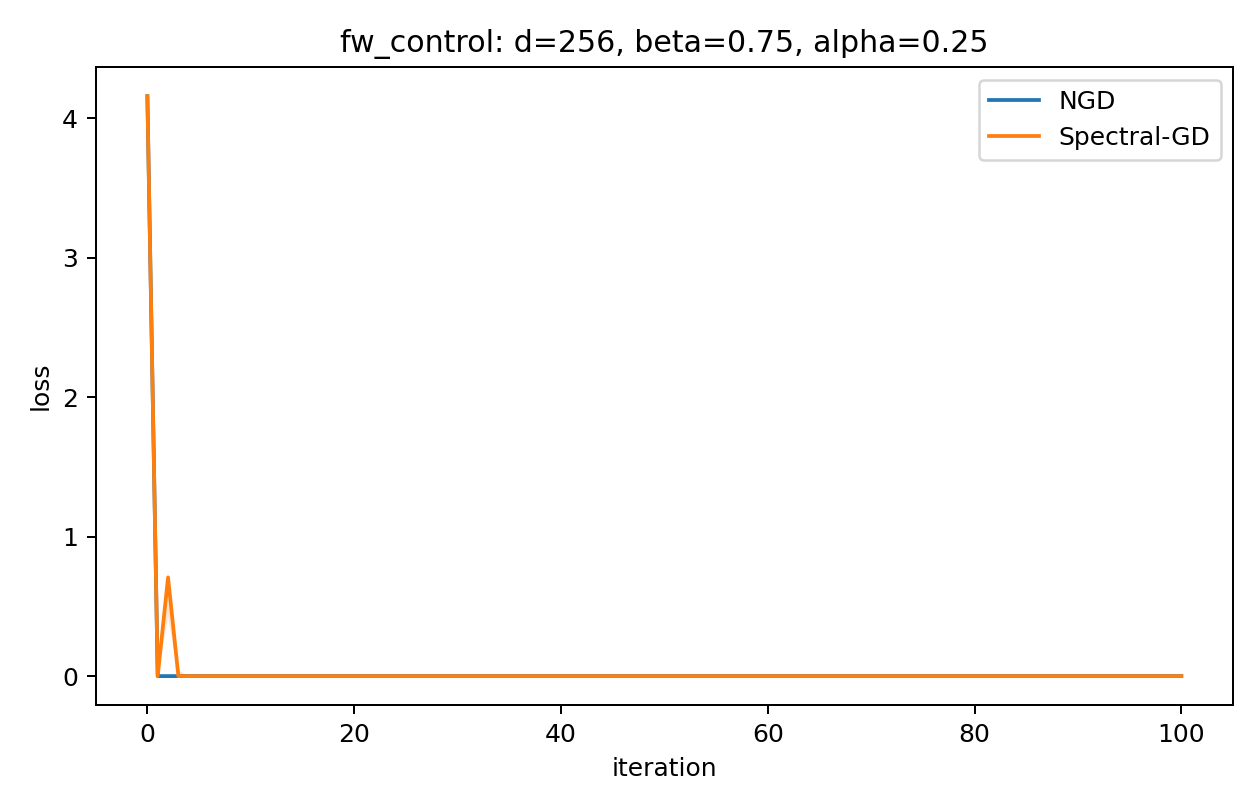
\includegraphics[width=\linewidth]{figures/loss_curves/fw_control_d256_b0.75_a0.25.png}
\caption{$\alpha=0.25$}
\end{subfigure}%
\hfill
\begin{subfigure}{0.22\textwidth}
\centering
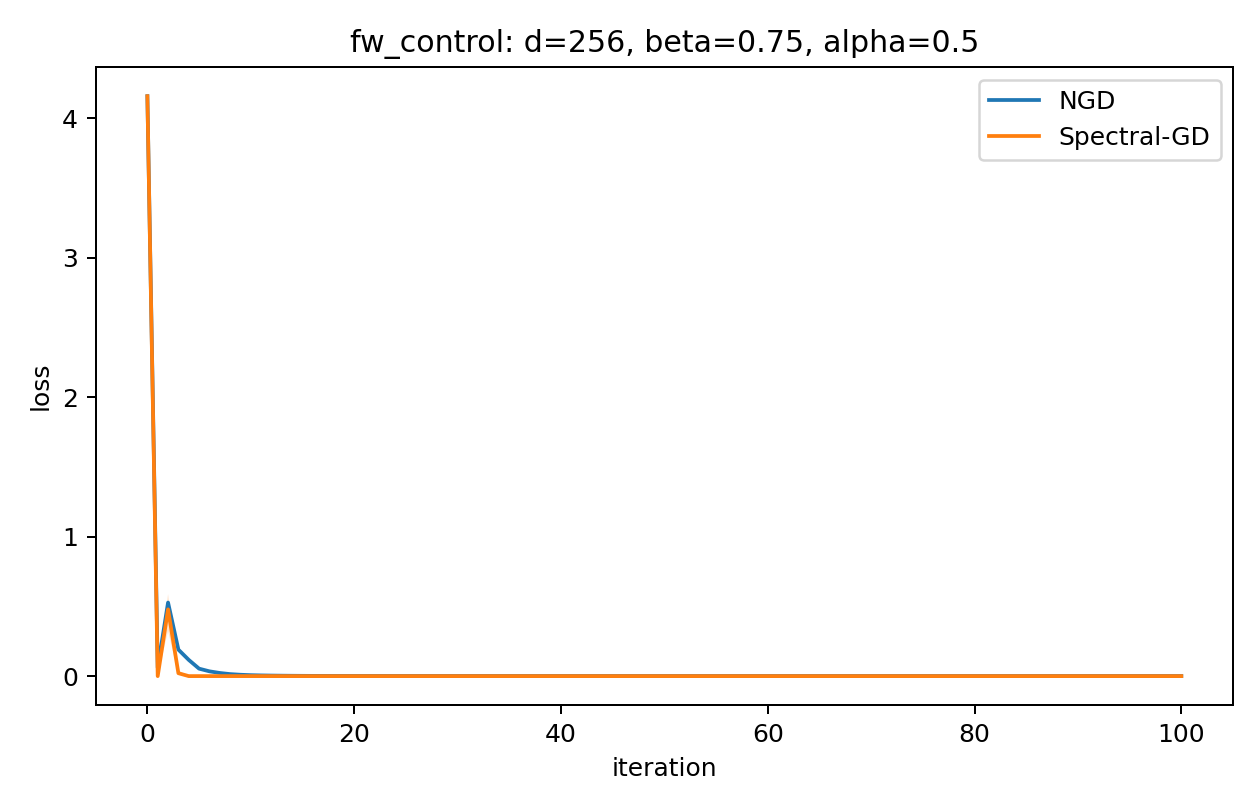
\includegraphics[width=\linewidth]{figures/loss_curves/fw_control_d256_b0.75_a0.5.png}
\caption{$\alpha=0.5$}
\end{subfigure}%
\hfill
\begin{subfigure}{0.22\textwidth}
\centering
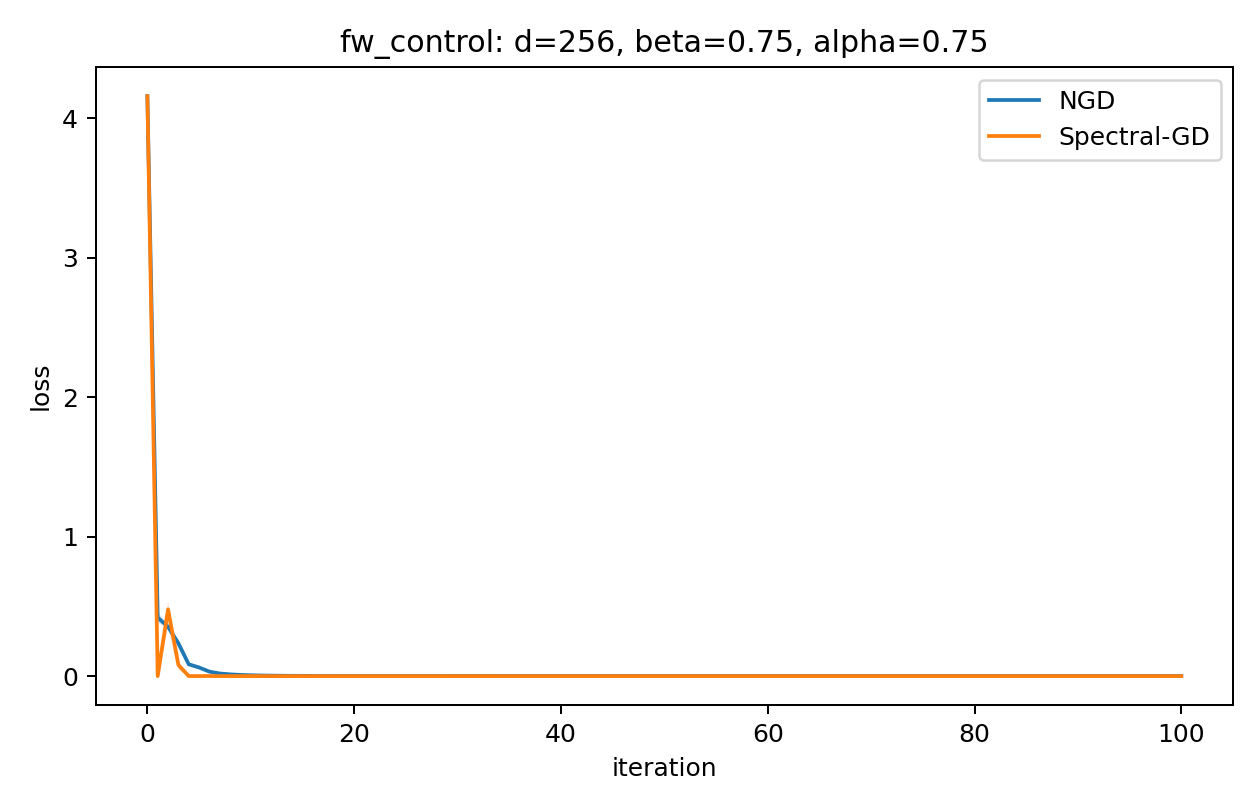
\includegraphics[width=\linewidth]{figures/loss_curves/fw_control_d256_b0.75_a0.75.png}
\caption{$\alpha=0.75$}
\end{subfigure}%
\par\smallskip
\begin{subfigure}{0.22\textwidth}
\centering
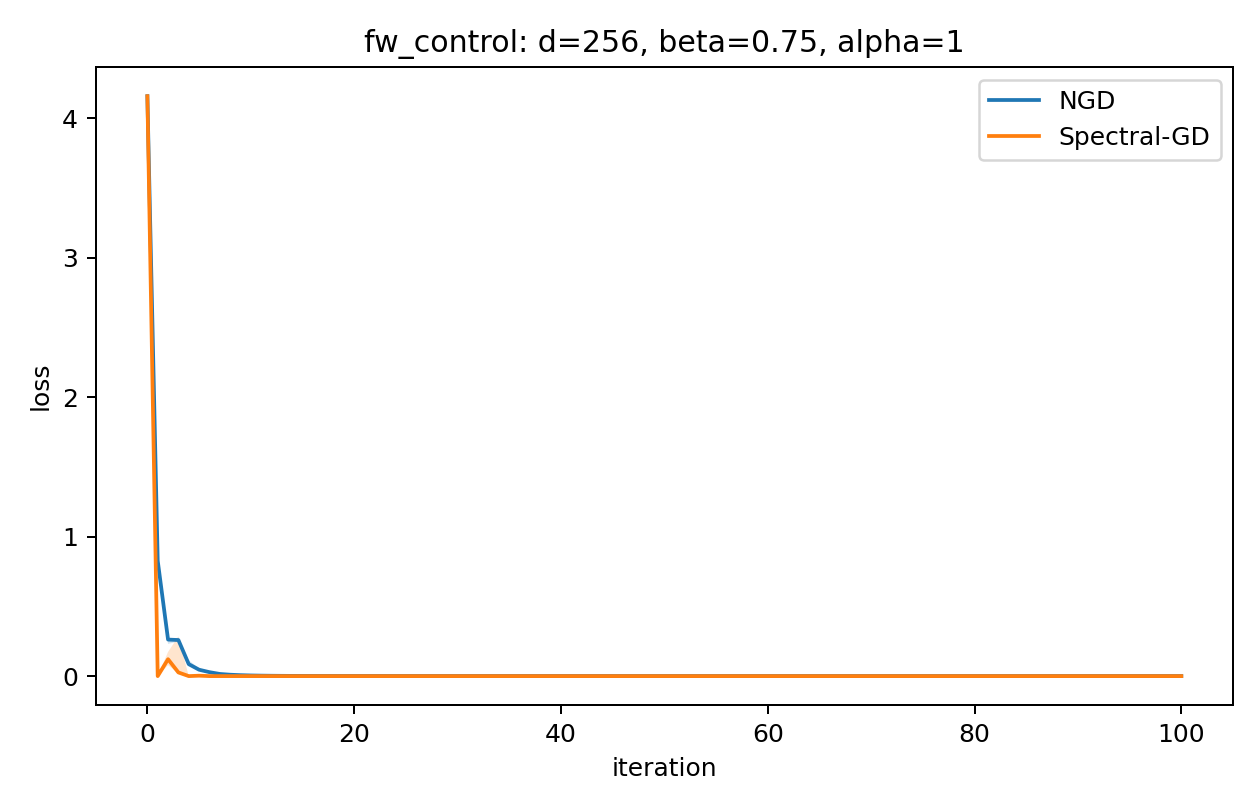
\includegraphics[width=\linewidth]{figures/loss_curves/fw_control_d256_b0.75_a1.png}
\caption{$\alpha=1$}
\end{subfigure}%
\hfill
\begin{subfigure}{0.22\textwidth}
\centering
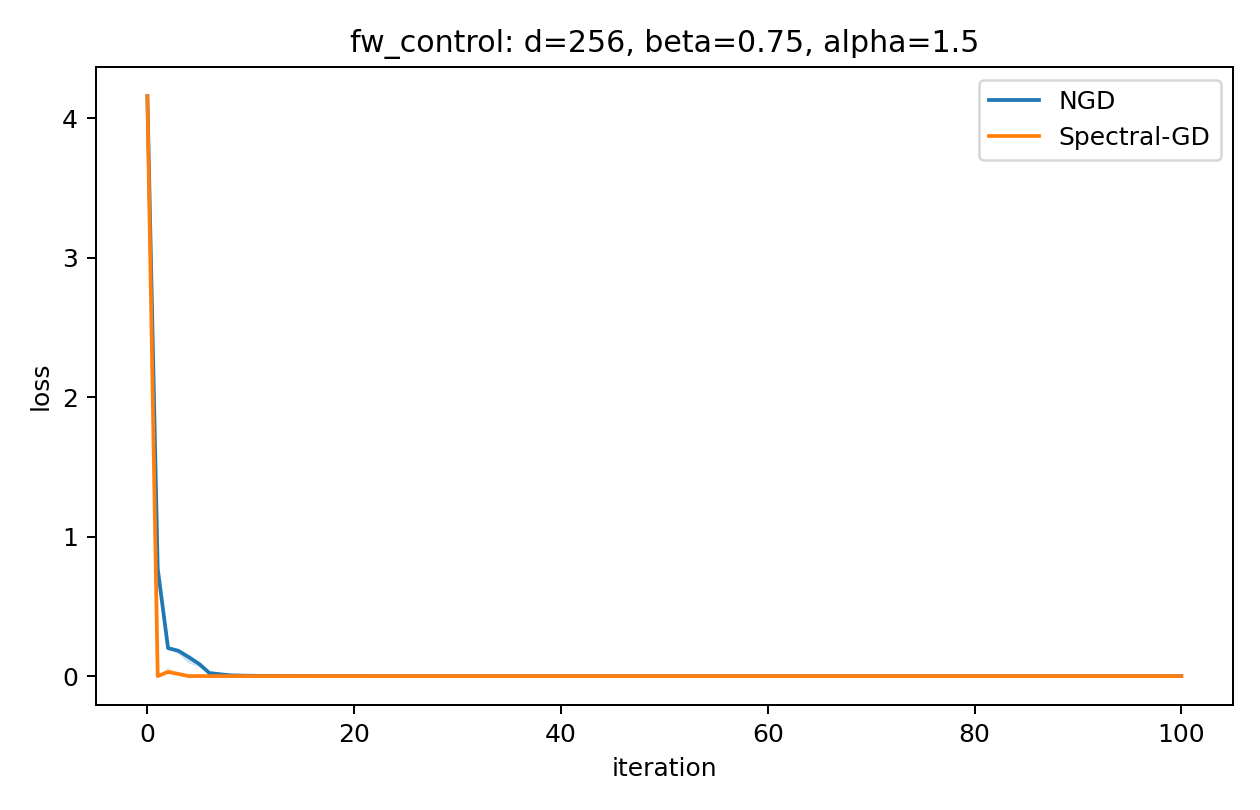
\includegraphics[width=\linewidth]{figures/loss_curves/fw_control_d256_b0.75_a1.5.png}
\caption{$\alpha=1.5$}
\end{subfigure}%
\hfill
\begin{subfigure}{0.22\textwidth}
\centering
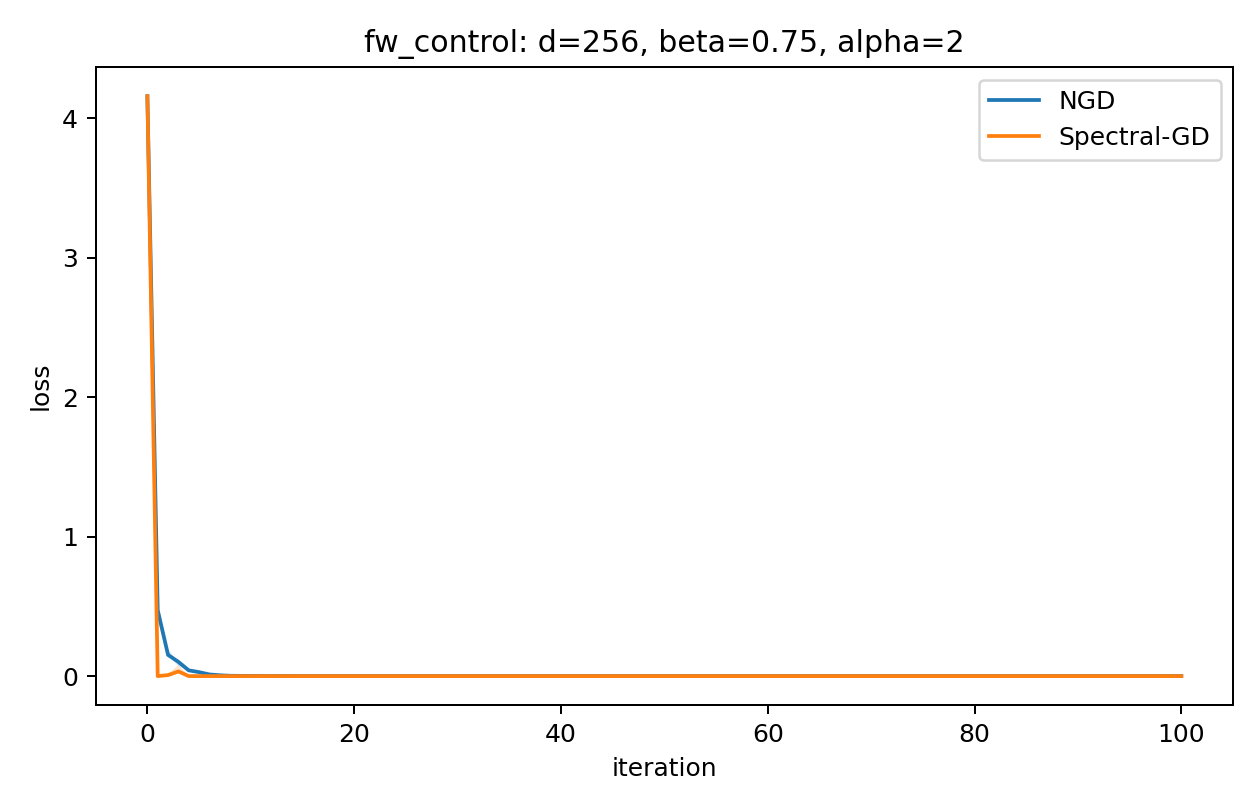
\includegraphics[width=\linewidth]{figures/loss_curves/fw_control_d256_b0.75_a2.png}
\caption{$\alpha=2$}
\end{subfigure}%
\caption{Best-auc loss curves for FW-control, $\beta=0.75$, $d=256$, $N=64$. Each panel is one value of $\alpha$. The solid line is the seed median and the shaded band is the interquartile range over three seeds.}
\label{fig:fw_control:loss:b075}
\end{figure}


\begin{figure}[H]
\centering
\begin{subfigure}{0.22\textwidth}
\centering

\includegraphics[width=\linewidth]{figures/loss_envelope_curves/fw_control_d256_b0.75_a0.png}
\caption{$\alpha=0$}
\end{subfigure}%
\hfill
\begin{subfigure}{0.22\textwidth}
\centering

\includegraphics[width=\linewidth]{figures/loss_envelope_curves/fw_control_d256_b0.75_a0.25.png}
\caption{$\alpha=0.25$}
\end{subfigure}%
\hfill
\begin{subfigure}{0.22\textwidth}
\centering

\includegraphics[width=\linewidth]{figures/loss_envelope_curves/fw_control_d256_b0.75_a0.5.png}
\caption{$\alpha=0.5$}
\end{subfigure}%
\hfill
\begin{subfigure}{0.22\textwidth}
\centering

\includegraphics[width=\linewidth]{figures/loss_envelope_curves/fw_control_d256_b0.75_a0.75.png}
\caption{$\alpha=0.75$}
\end{subfigure}%
\par\smallskip
\begin{subfigure}{0.22\textwidth}
\centering

\includegraphics[width=\linewidth]{figures/loss_envelope_curves/fw_control_d256_b0.75_a1.png}
\caption{$\alpha=1$}
\end{subfigure}%
\hfill
\begin{subfigure}{0.22\textwidth}
\centering

\includegraphics[width=\linewidth]{figures/loss_envelope_curves/fw_control_d256_b0.75_a1.5.png}
\caption{$\alpha=1.5$}
\end{subfigure}%
\hfill
\begin{subfigure}{0.22\textwidth}
\centering

\includegraphics[width=\linewidth]{figures/loss_envelope_curves/fw_control_d256_b0.75_a2.png}
\caption{$\alpha=2$}
\end{subfigure}%
\caption{Loss envelope curves for FW-control, $\beta=0.75$, $d=256$, $N=64$. Each panel is one value of $\alpha$. The solid line is the seed median and the shaded band is the interquartile range over three seeds.}
\label{fig:fw_control:envelope:b075}
\end{figure}


\begin{figure}[H]
\centering
\begin{subfigure}{0.22\textwidth}
\centering
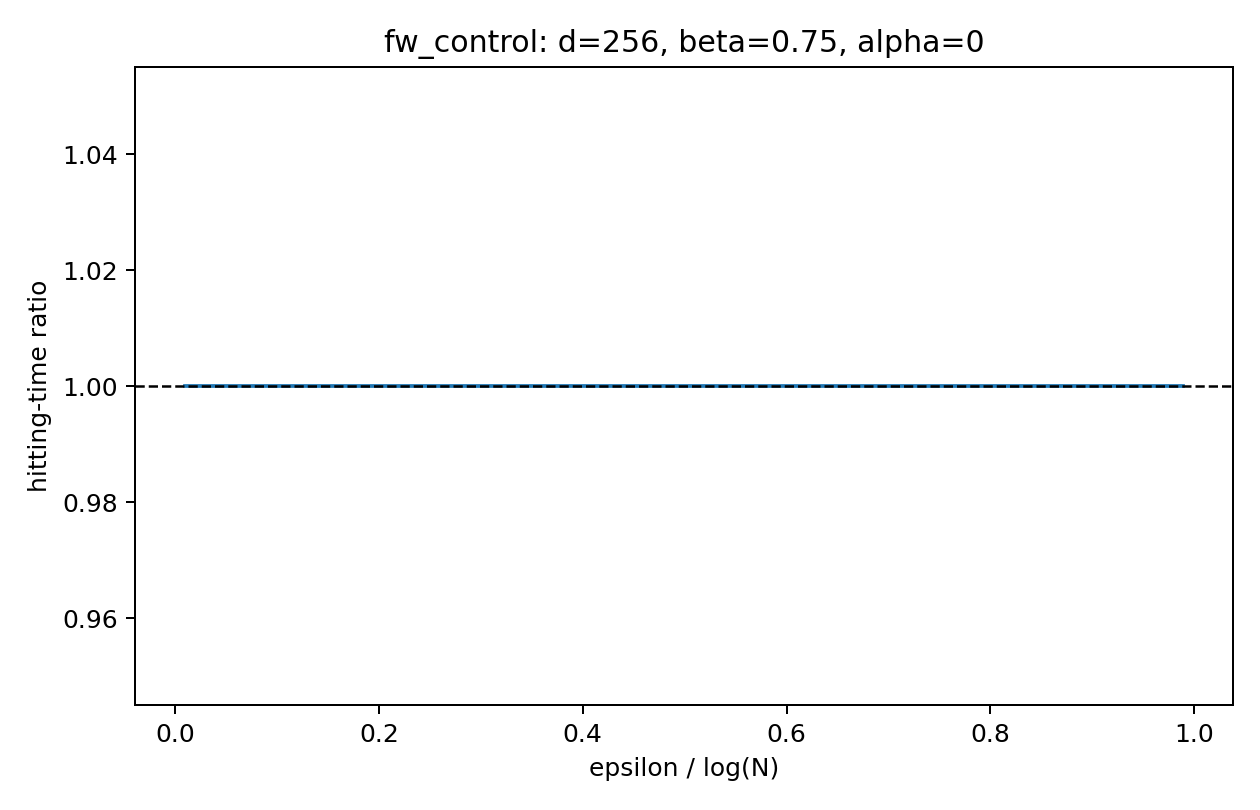
\includegraphics[width=\linewidth]{figures/ratio_curves/T_ratio_fw_control_d256_b0.75_a0.png}
\caption{$\alpha=0$}
\end{subfigure}%
\hfill
\begin{subfigure}{0.22\textwidth}
\centering
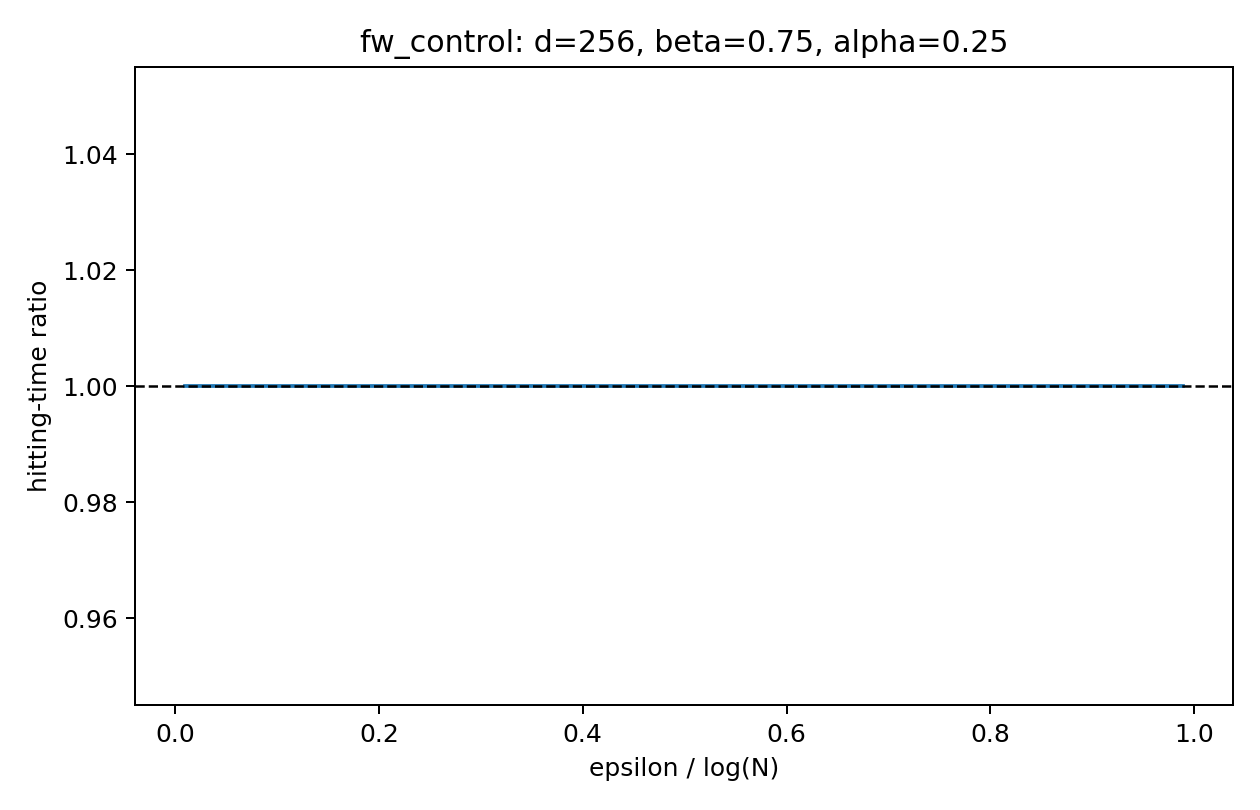
\includegraphics[width=\linewidth]{figures/ratio_curves/T_ratio_fw_control_d256_b0.75_a0.25.png}
\caption{$\alpha=0.25$}
\end{subfigure}%
\hfill
\begin{subfigure}{0.22\textwidth}
\centering
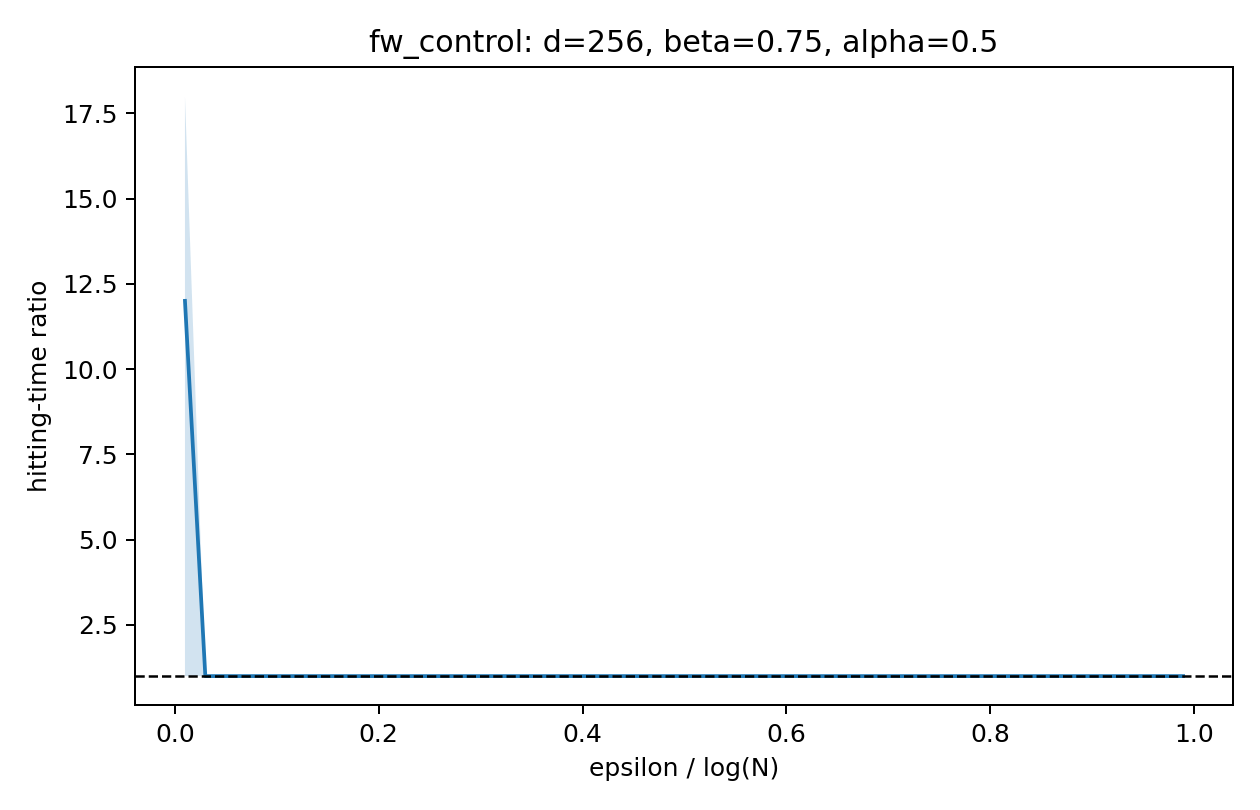
\includegraphics[width=\linewidth]{figures/ratio_curves/T_ratio_fw_control_d256_b0.75_a0.5.png}
\caption{$\alpha=0.5$}
\end{subfigure}%
\hfill
\begin{subfigure}{0.22\textwidth}
\centering
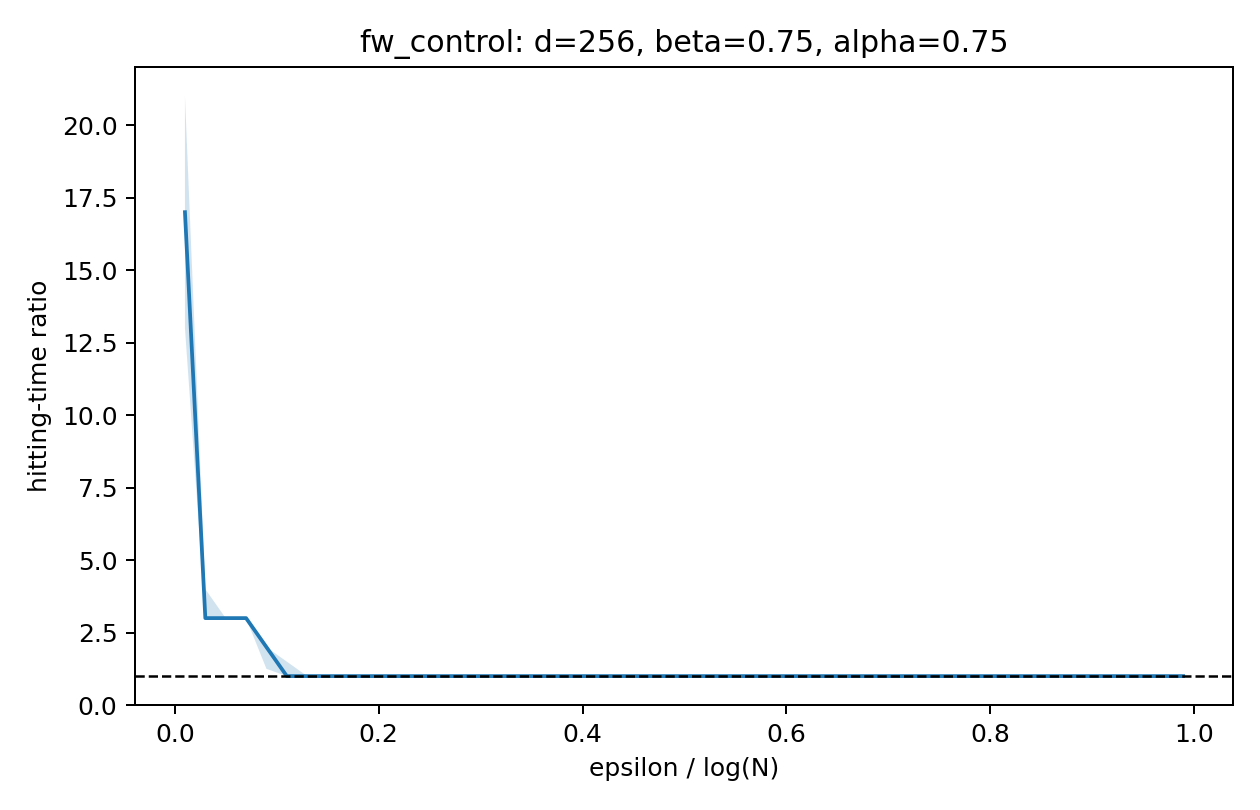
\includegraphics[width=\linewidth]{figures/ratio_curves/T_ratio_fw_control_d256_b0.75_a0.75.png}
\caption{$\alpha=0.75$}
\end{subfigure}%
\par\smallskip
\begin{subfigure}{0.22\textwidth}
\centering
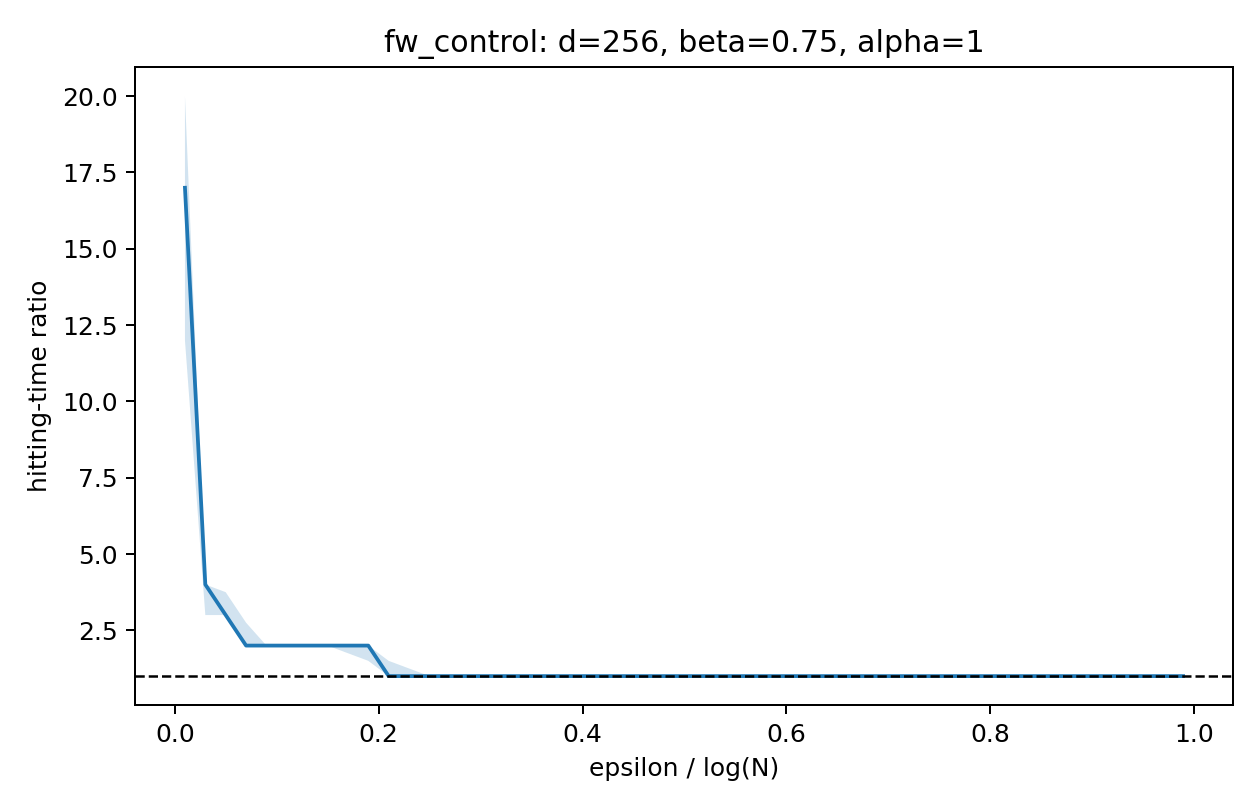
\includegraphics[width=\linewidth]{figures/ratio_curves/T_ratio_fw_control_d256_b0.75_a1.png}
\caption{$\alpha=1$}
\end{subfigure}%
\hfill
\begin{subfigure}{0.22\textwidth}
\centering
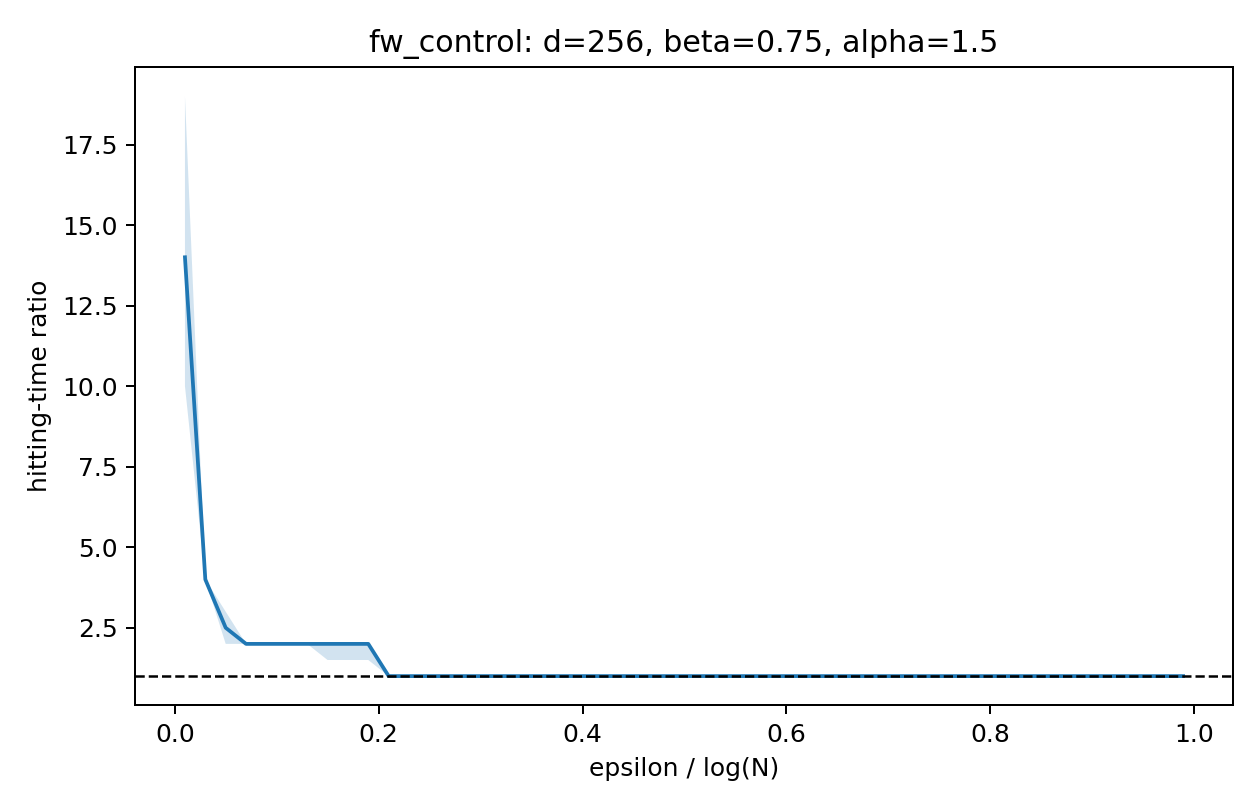
\includegraphics[width=\linewidth]{figures/ratio_curves/T_ratio_fw_control_d256_b0.75_a1.5.png}
\caption{$\alpha=1.5$}
\end{subfigure}%
\hfill
\begin{subfigure}{0.22\textwidth}
\centering
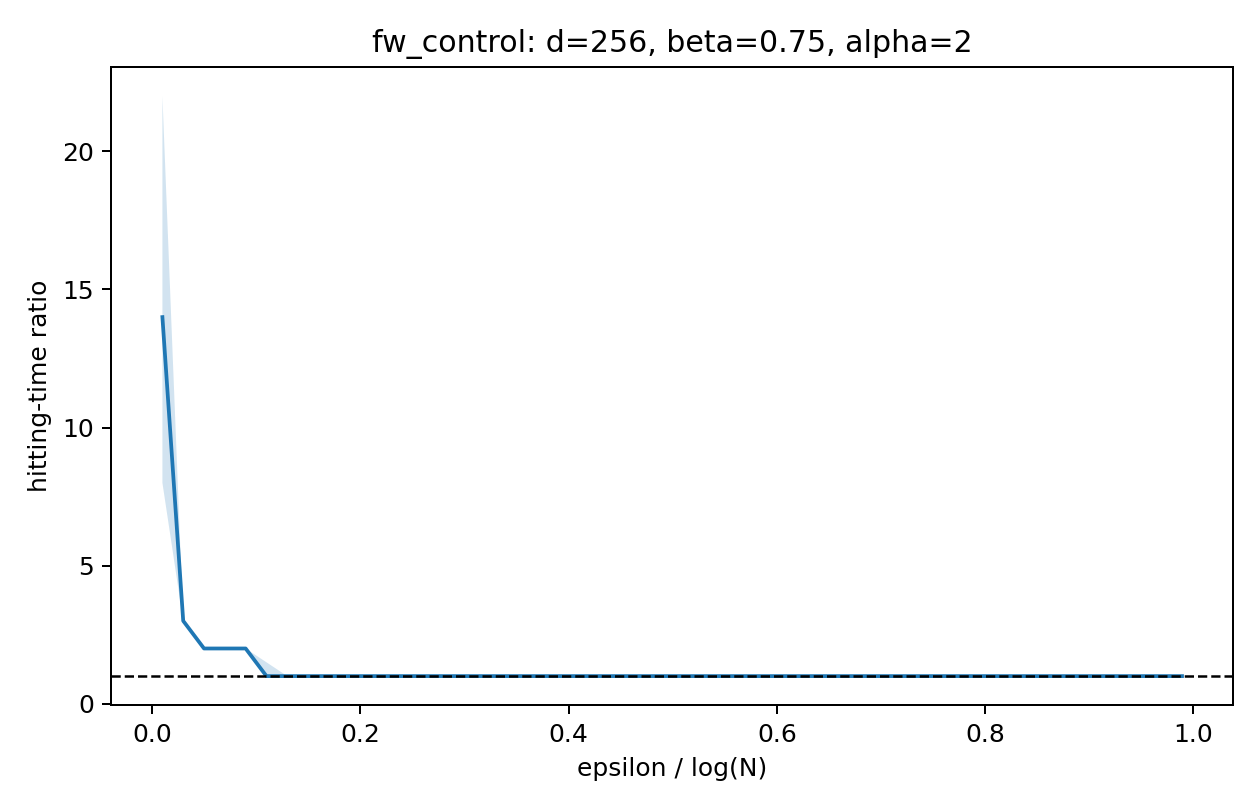
\includegraphics[width=\linewidth]{figures/ratio_curves/T_ratio_fw_control_d256_b0.75_a2.png}
\caption{$\alpha=2$}
\end{subfigure}%
\caption{Hitting-time ratio curves for FW-control, $\beta=0.75$, $d=256$, $N=64$. Each panel is one value of $\alpha$. The solid line is the seed median and the shaded band is the interquartile range over three seeds.}
\label{fig:fw_control:T_ratio:b075}
\end{figure}






\subsubsection{$\beta=1.25$, $d=256$, $N=1024$}

The following three figures show the complete alpha sweep for this beta block: the best-AUC loss traces, the per-step hyperparameter envelope, and the hitting-time ratio. Reading them together is important: the loss curves show ordinary tuned trajectories, the envelope shows the best loss achievable at each iteration under the sweep, and the hitting-time ratio is the primary speed metric.

\begin{figure}[H]
\centering
\begin{subfigure}{0.22\textwidth}
\centering
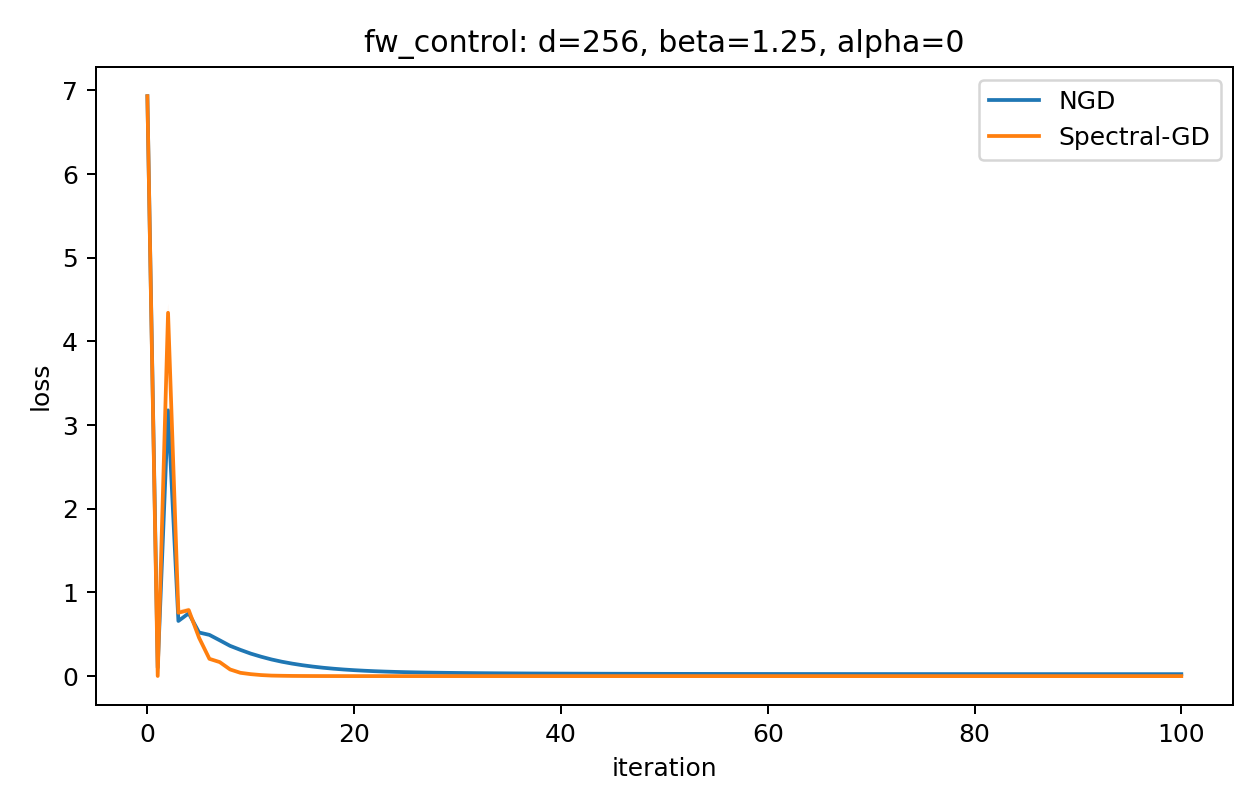
\includegraphics[width=\linewidth]{figures/loss_curves/fw_control_d256_b1.25_a0.png}
\caption{$\alpha=0$}
\end{subfigure}%
\hfill
\begin{subfigure}{0.22\textwidth}
\centering
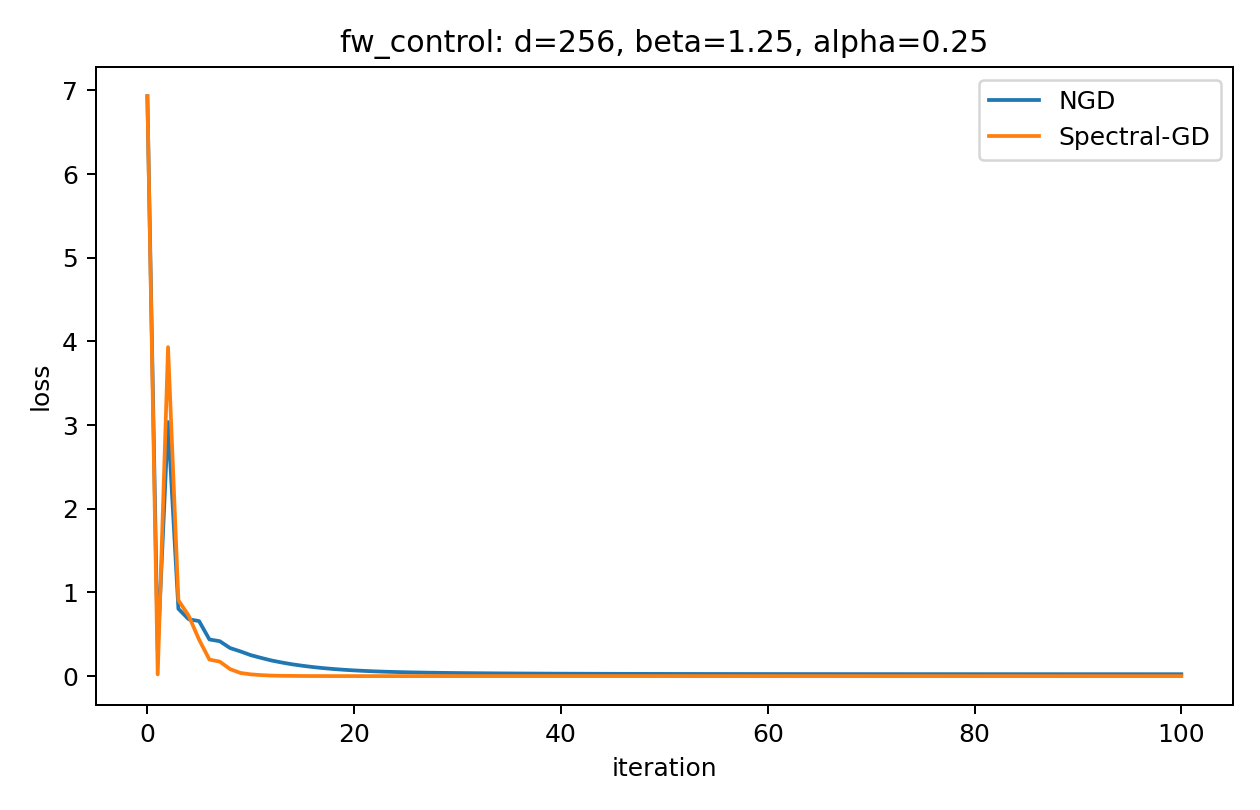
\includegraphics[width=\linewidth]{figures/loss_curves/fw_control_d256_b1.25_a0.25.png}
\caption{$\alpha=0.25$}
\end{subfigure}%
\hfill
\begin{subfigure}{0.22\textwidth}
\centering
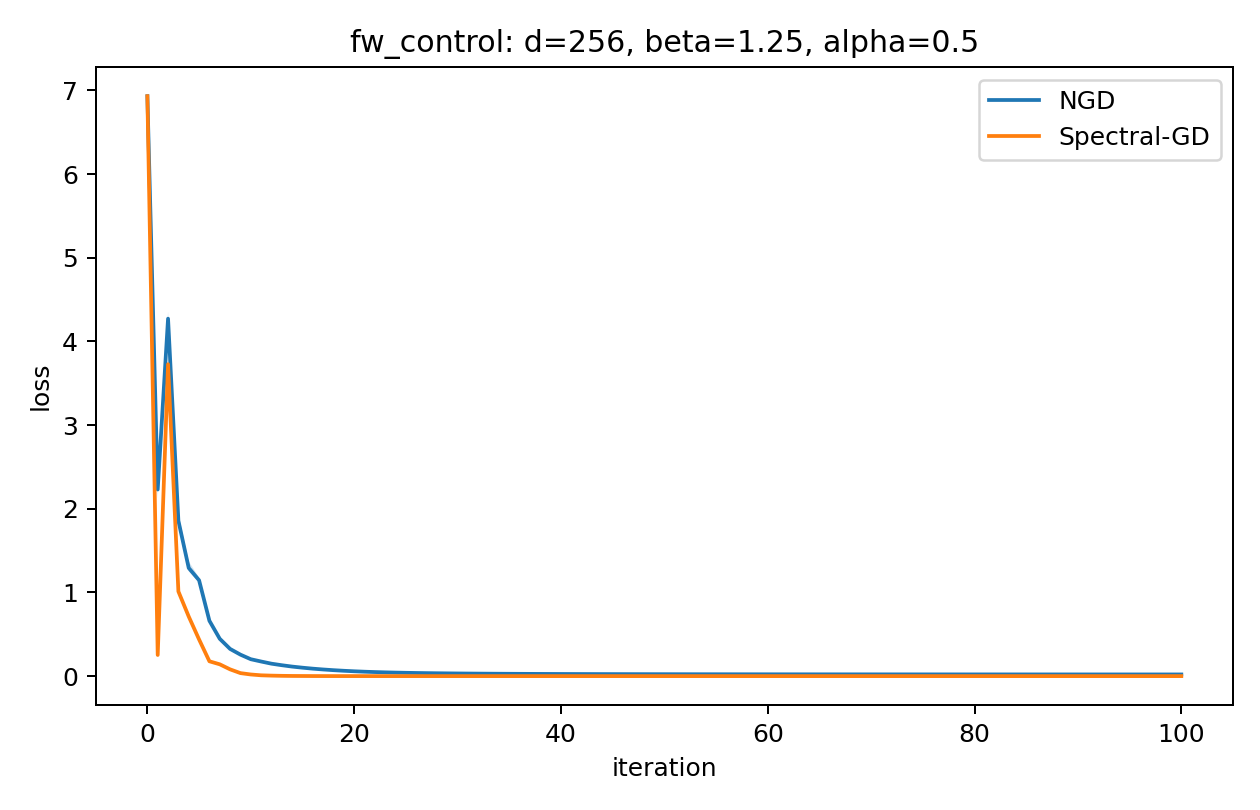
\includegraphics[width=\linewidth]{figures/loss_curves/fw_control_d256_b1.25_a0.5.png}
\caption{$\alpha=0.5$}
\end{subfigure}%
\hfill
\begin{subfigure}{0.22\textwidth}
\centering
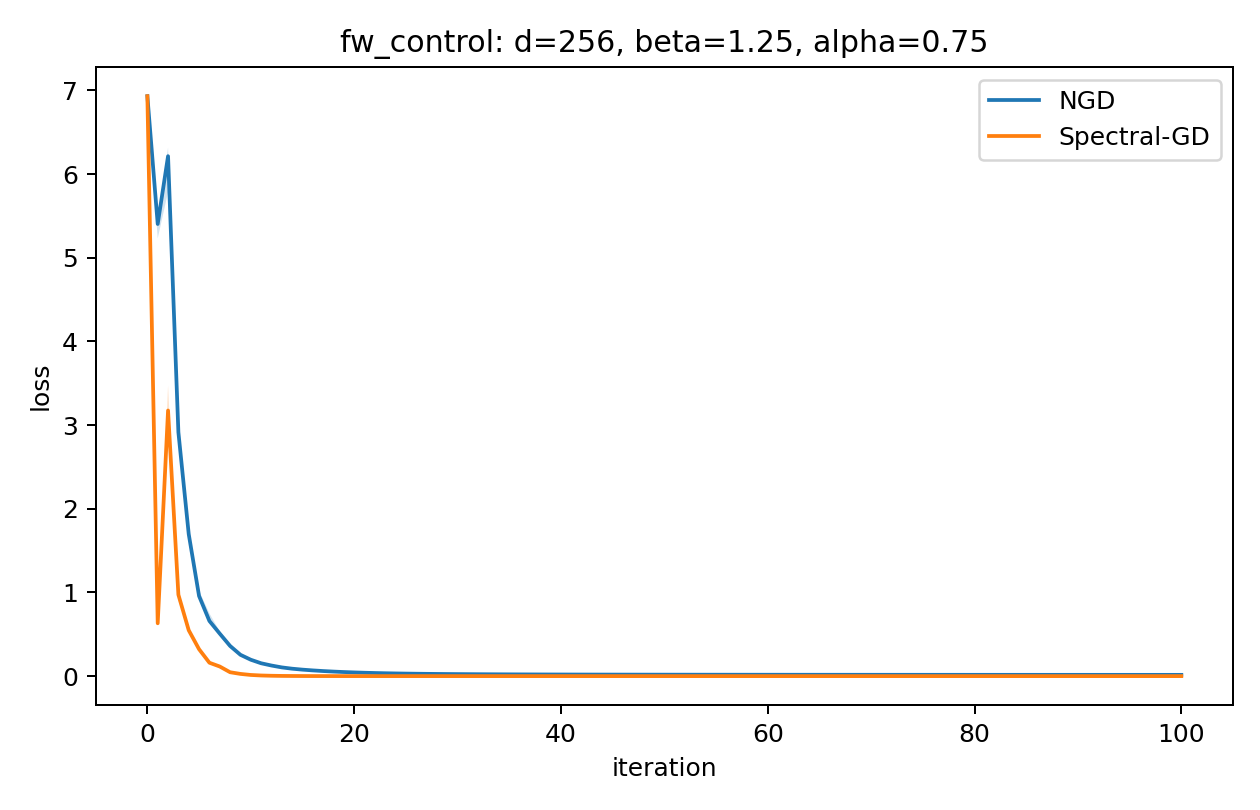
\includegraphics[width=\linewidth]{figures/loss_curves/fw_control_d256_b1.25_a0.75.png}
\caption{$\alpha=0.75$}
\end{subfigure}%
\par\smallskip
\begin{subfigure}{0.22\textwidth}
\centering
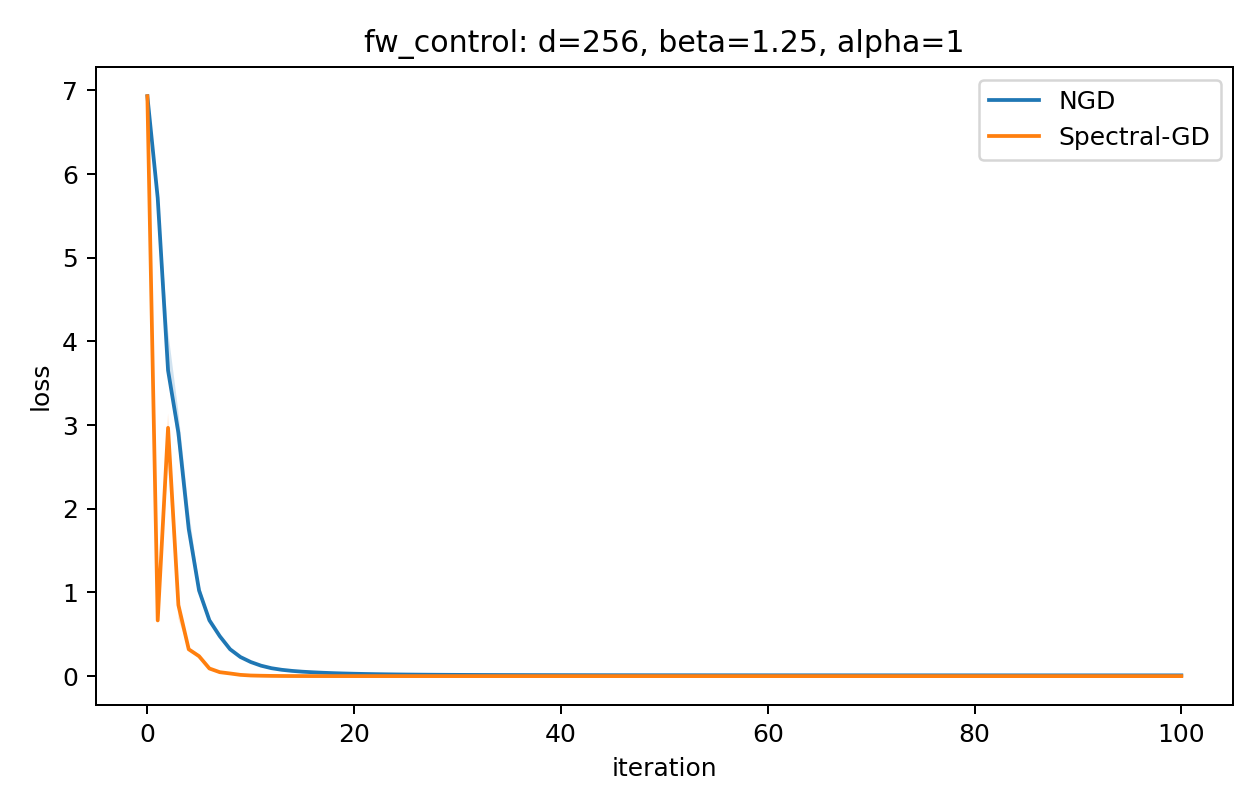
\includegraphics[width=\linewidth]{figures/loss_curves/fw_control_d256_b1.25_a1.png}
\caption{$\alpha=1$}
\end{subfigure}%
\hfill
\begin{subfigure}{0.22\textwidth}
\centering
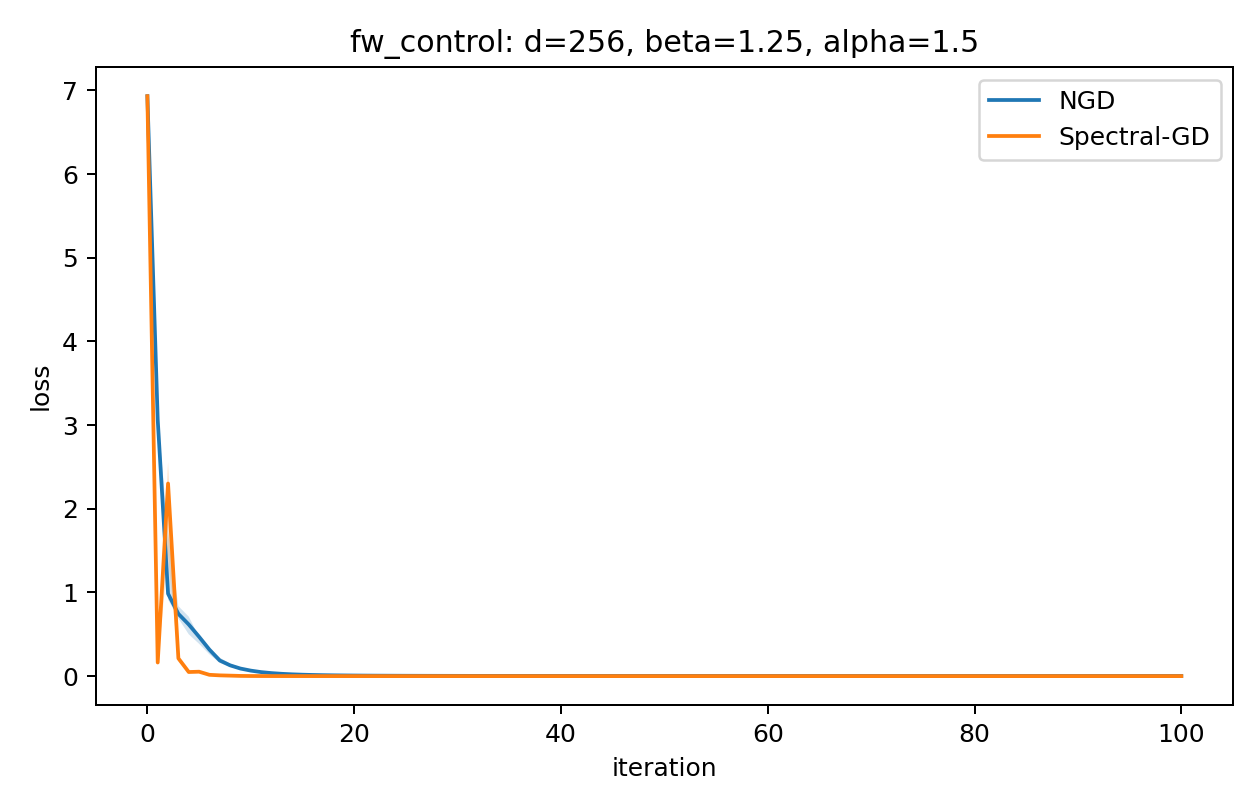
\includegraphics[width=\linewidth]{figures/loss_curves/fw_control_d256_b1.25_a1.5.png}
\caption{$\alpha=1.5$}
\end{subfigure}%
\hfill
\begin{subfigure}{0.22\textwidth}
\centering
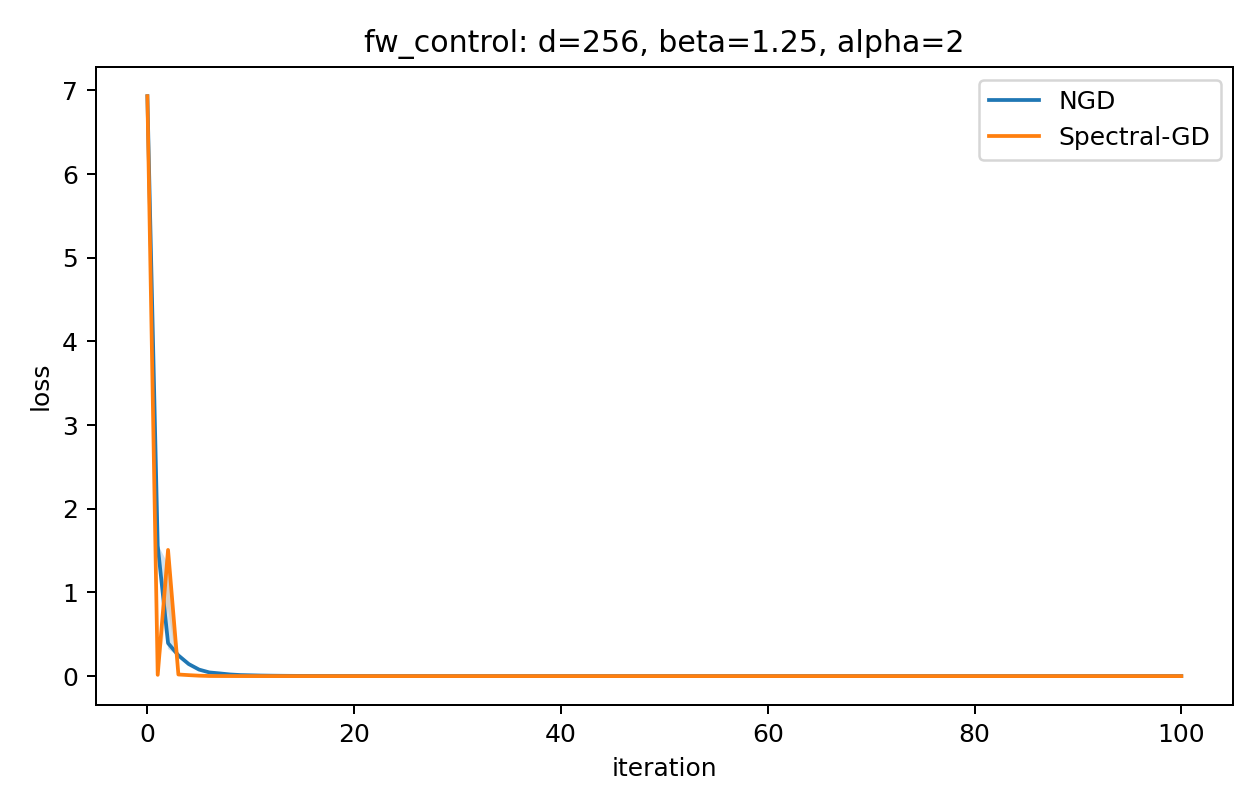
\includegraphics[width=\linewidth]{figures/loss_curves/fw_control_d256_b1.25_a2.png}
\caption{$\alpha=2$}
\end{subfigure}%
\caption{Best-auc loss curves for FW-control, $\beta=1.25$, $d=256$, $N=1024$. Each panel is one value of $\alpha$. The solid line is the seed median and the shaded band is the interquartile range over three seeds.}
\label{fig:fw_control:loss:b125}
\end{figure}


\begin{figure}[H]
\centering
\begin{subfigure}{0.22\textwidth}
\centering

\includegraphics[width=\linewidth]{figures/loss_envelope_curves/fw_control_d256_b1.25_a0.png}
\caption{$\alpha=0$}
\end{subfigure}%
\hfill
\begin{subfigure}{0.22\textwidth}
\centering

\includegraphics[width=\linewidth]{figures/loss_envelope_curves/fw_control_d256_b1.25_a0.25.png}
\caption{$\alpha=0.25$}
\end{subfigure}%
\hfill
\begin{subfigure}{0.22\textwidth}
\centering

\includegraphics[width=\linewidth]{figures/loss_envelope_curves/fw_control_d256_b1.25_a0.5.png}
\caption{$\alpha=0.5$}
\end{subfigure}%
\hfill
\begin{subfigure}{0.22\textwidth}
\centering

\includegraphics[width=\linewidth]{figures/loss_envelope_curves/fw_control_d256_b1.25_a0.75.png}
\caption{$\alpha=0.75$}
\end{subfigure}%
\par\smallskip
\begin{subfigure}{0.22\textwidth}
\centering

\includegraphics[width=\linewidth]{figures/loss_envelope_curves/fw_control_d256_b1.25_a1.png}
\caption{$\alpha=1$}
\end{subfigure}%
\hfill
\begin{subfigure}{0.22\textwidth}
\centering

\includegraphics[width=\linewidth]{figures/loss_envelope_curves/fw_control_d256_b1.25_a1.5.png}
\caption{$\alpha=1.5$}
\end{subfigure}%
\hfill
\begin{subfigure}{0.22\textwidth}
\centering

\includegraphics[width=\linewidth]{figures/loss_envelope_curves/fw_control_d256_b1.25_a2.png}
\caption{$\alpha=2$}
\end{subfigure}%
\caption{Loss envelope curves for FW-control, $\beta=1.25$, $d=256$, $N=1024$. Each panel is one value of $\alpha$. The solid line is the seed median and the shaded band is the interquartile range over three seeds.}
\label{fig:fw_control:envelope:b125}
\end{figure}


\begin{figure}[H]
\centering
\begin{subfigure}{0.22\textwidth}
\centering
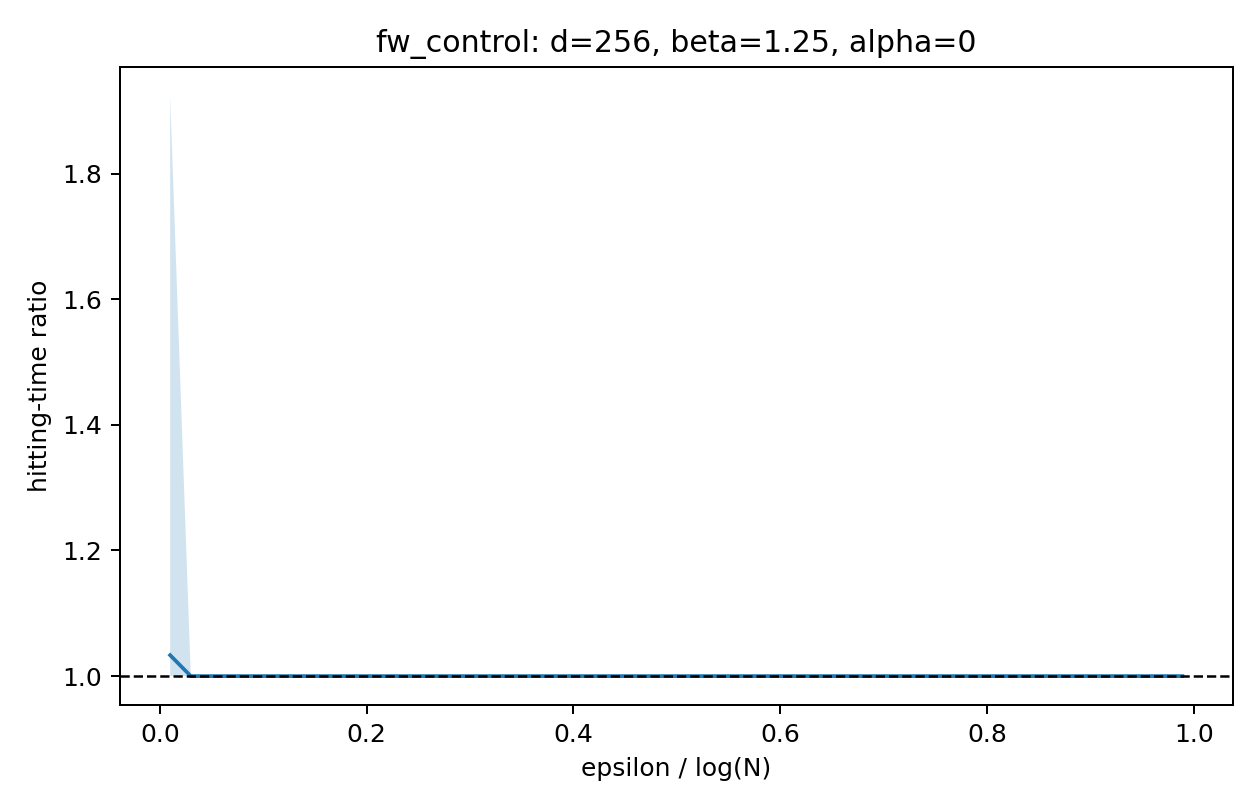
\includegraphics[width=\linewidth]{figures/ratio_curves/T_ratio_fw_control_d256_b1.25_a0.png}
\caption{$\alpha=0$}
\end{subfigure}%
\hfill
\begin{subfigure}{0.22\textwidth}
\centering
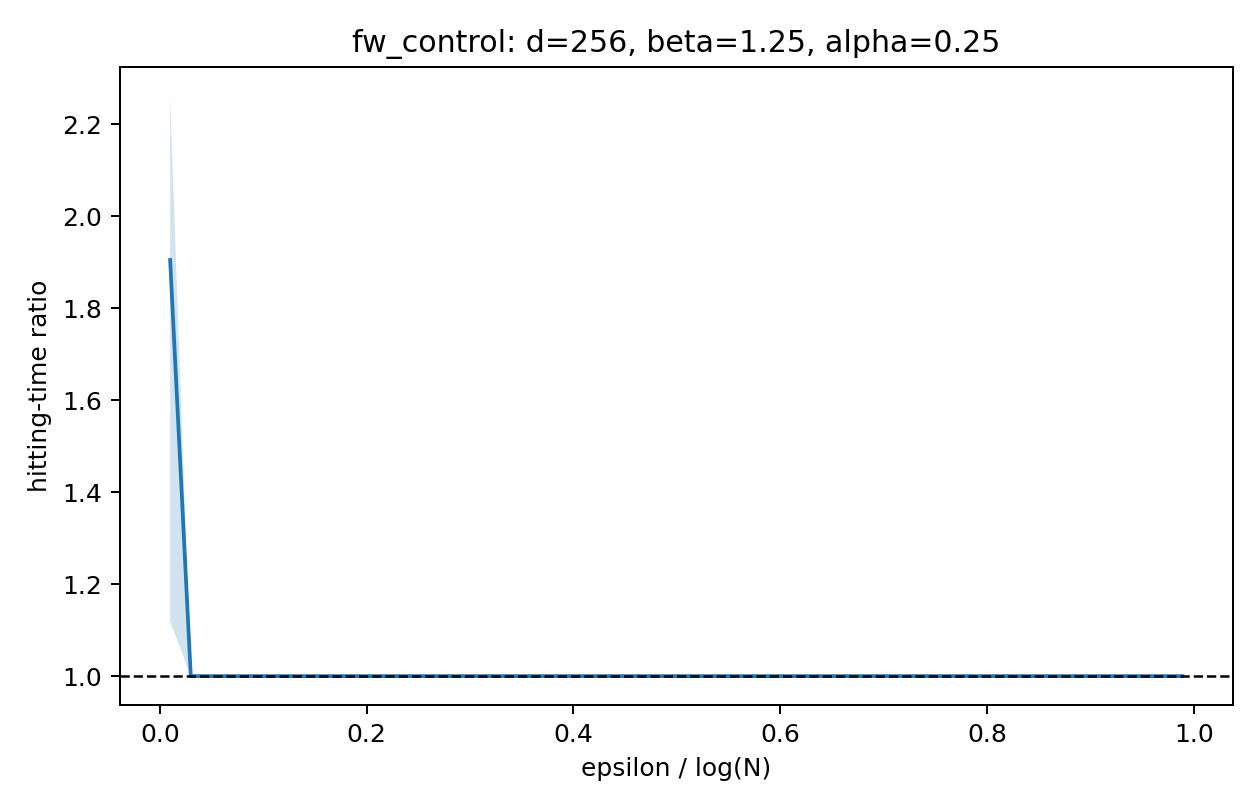
\includegraphics[width=\linewidth]{figures/ratio_curves/T_ratio_fw_control_d256_b1.25_a0.25.png}
\caption{$\alpha=0.25$}
\end{subfigure}%
\hfill
\begin{subfigure}{0.22\textwidth}
\centering
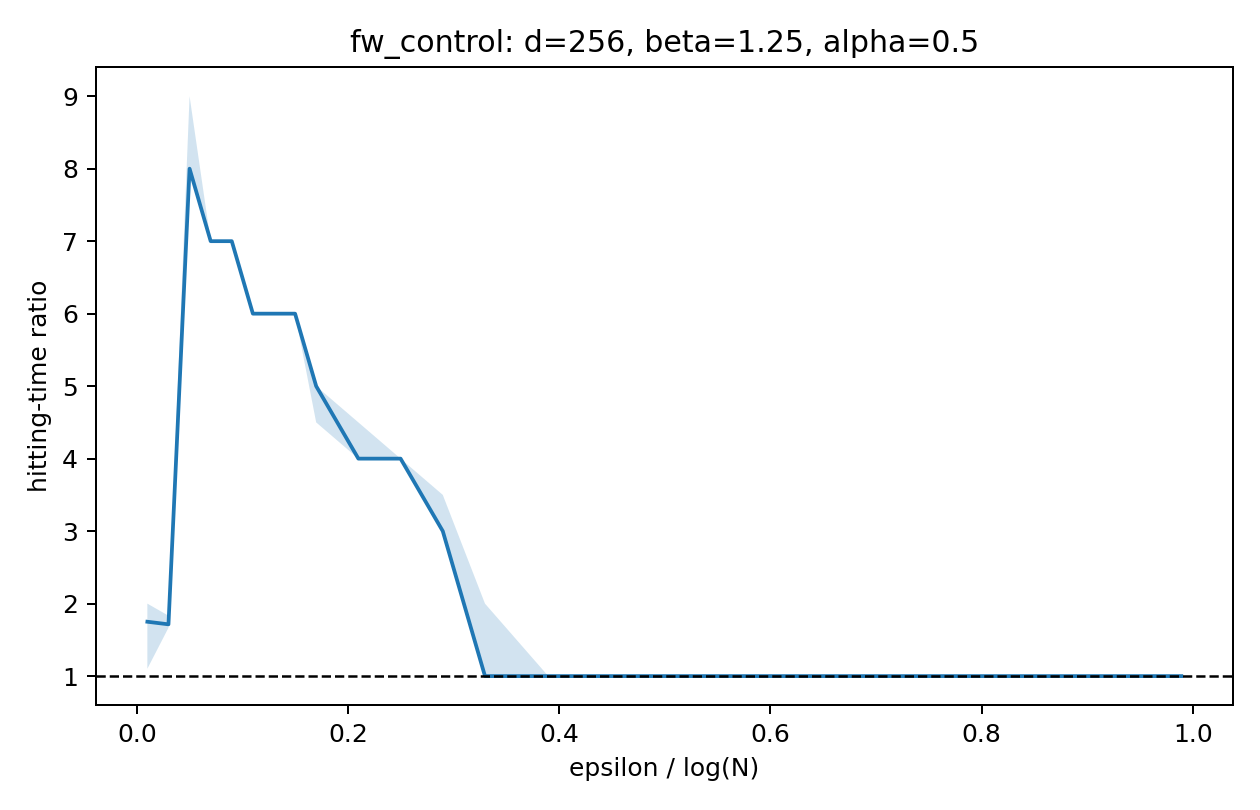
\includegraphics[width=\linewidth]{figures/ratio_curves/T_ratio_fw_control_d256_b1.25_a0.5.png}
\caption{$\alpha=0.5$}
\end{subfigure}%
\hfill
\begin{subfigure}{0.22\textwidth}
\centering
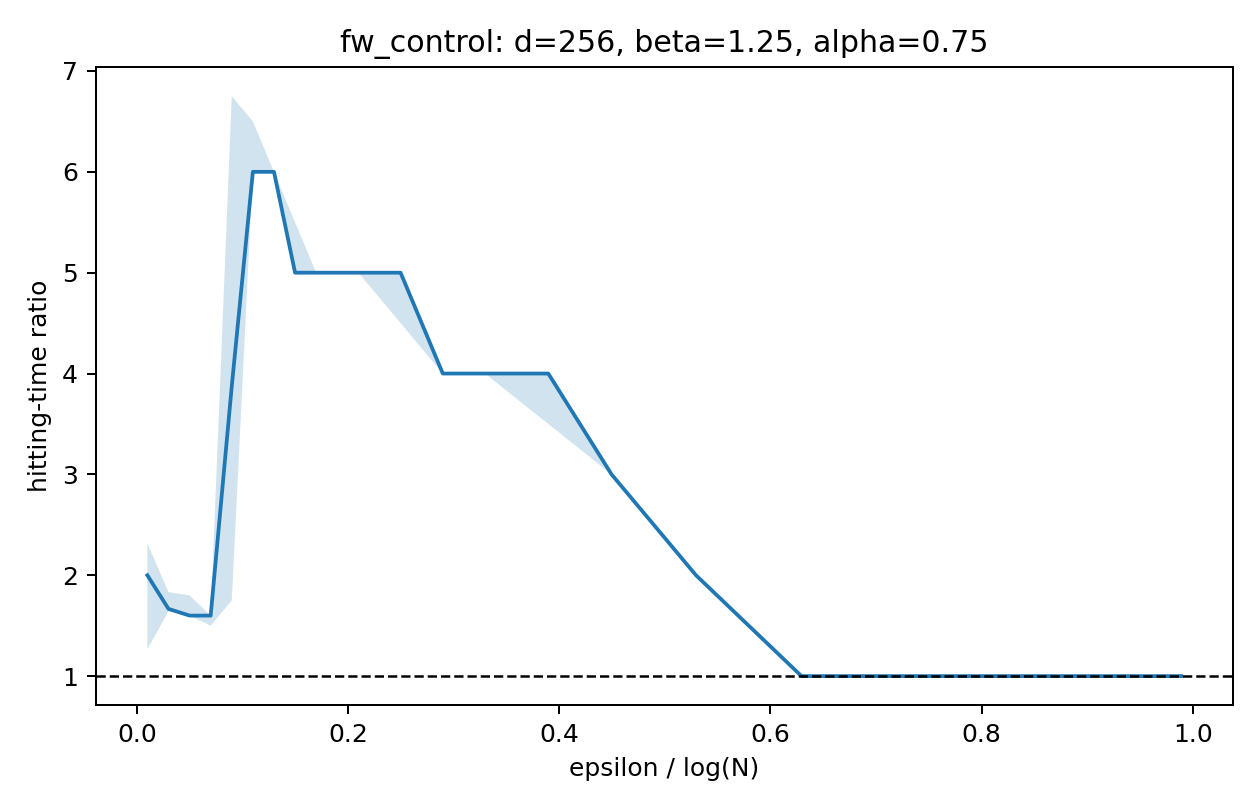
\includegraphics[width=\linewidth]{figures/ratio_curves/T_ratio_fw_control_d256_b1.25_a0.75.png}
\caption{$\alpha=0.75$}
\end{subfigure}%
\par\smallskip
\begin{subfigure}{0.22\textwidth}
\centering
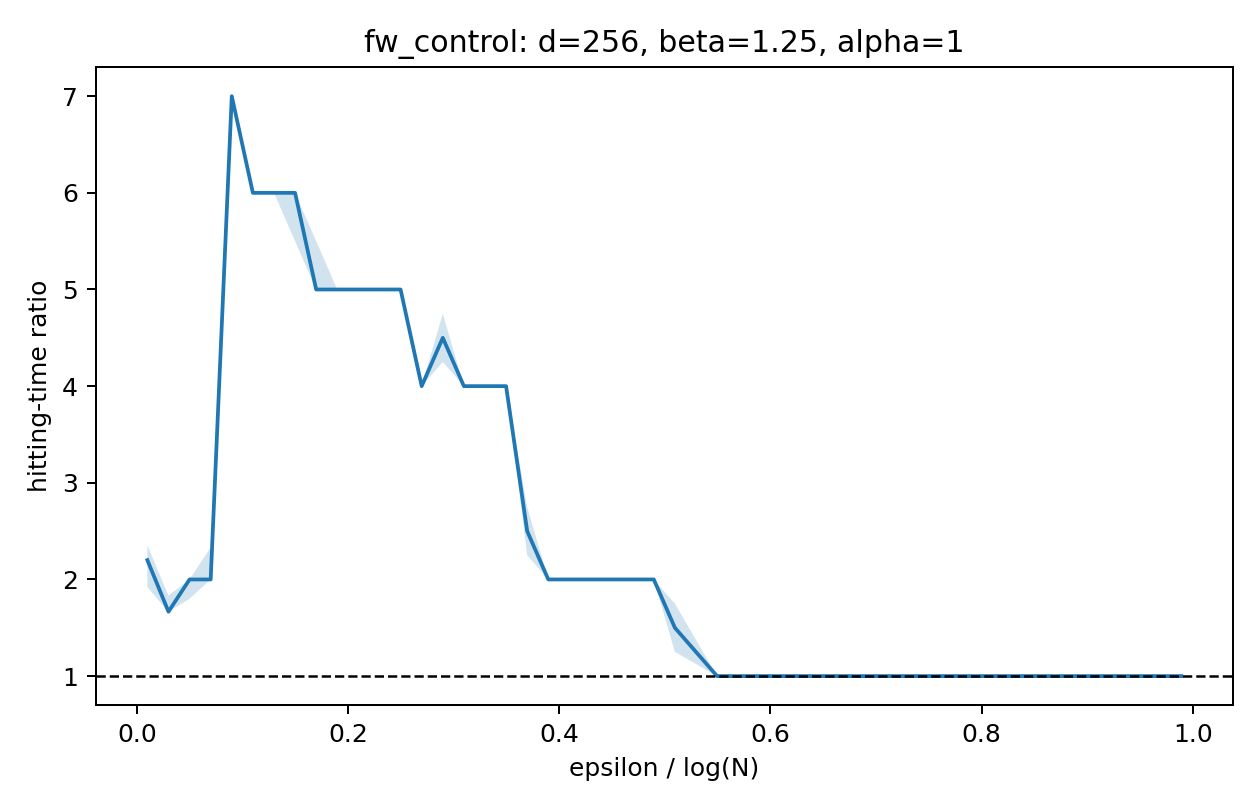
\includegraphics[width=\linewidth]{figures/ratio_curves/T_ratio_fw_control_d256_b1.25_a1.png}
\caption{$\alpha=1$}
\end{subfigure}%
\hfill
\begin{subfigure}{0.22\textwidth}
\centering
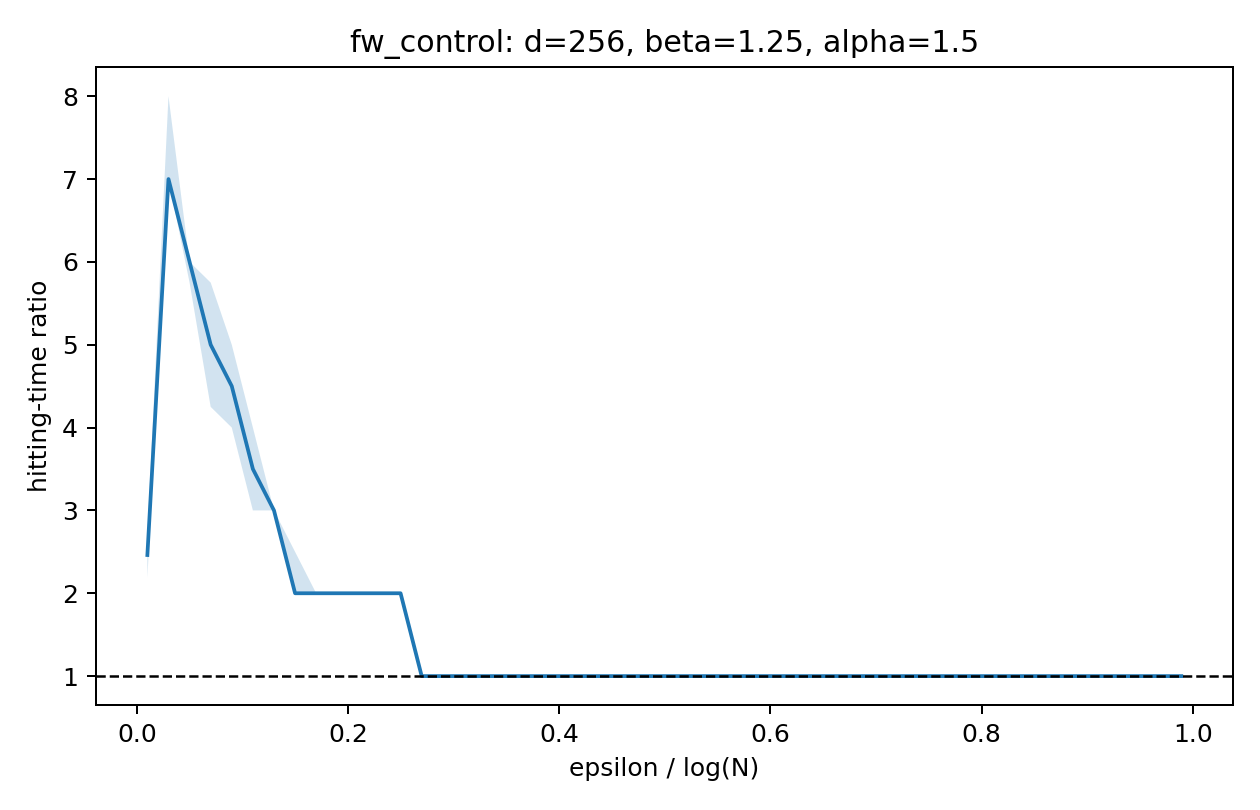
\includegraphics[width=\linewidth]{figures/ratio_curves/T_ratio_fw_control_d256_b1.25_a1.5.png}
\caption{$\alpha=1.5$}
\end{subfigure}%
\hfill
\begin{subfigure}{0.22\textwidth}
\centering
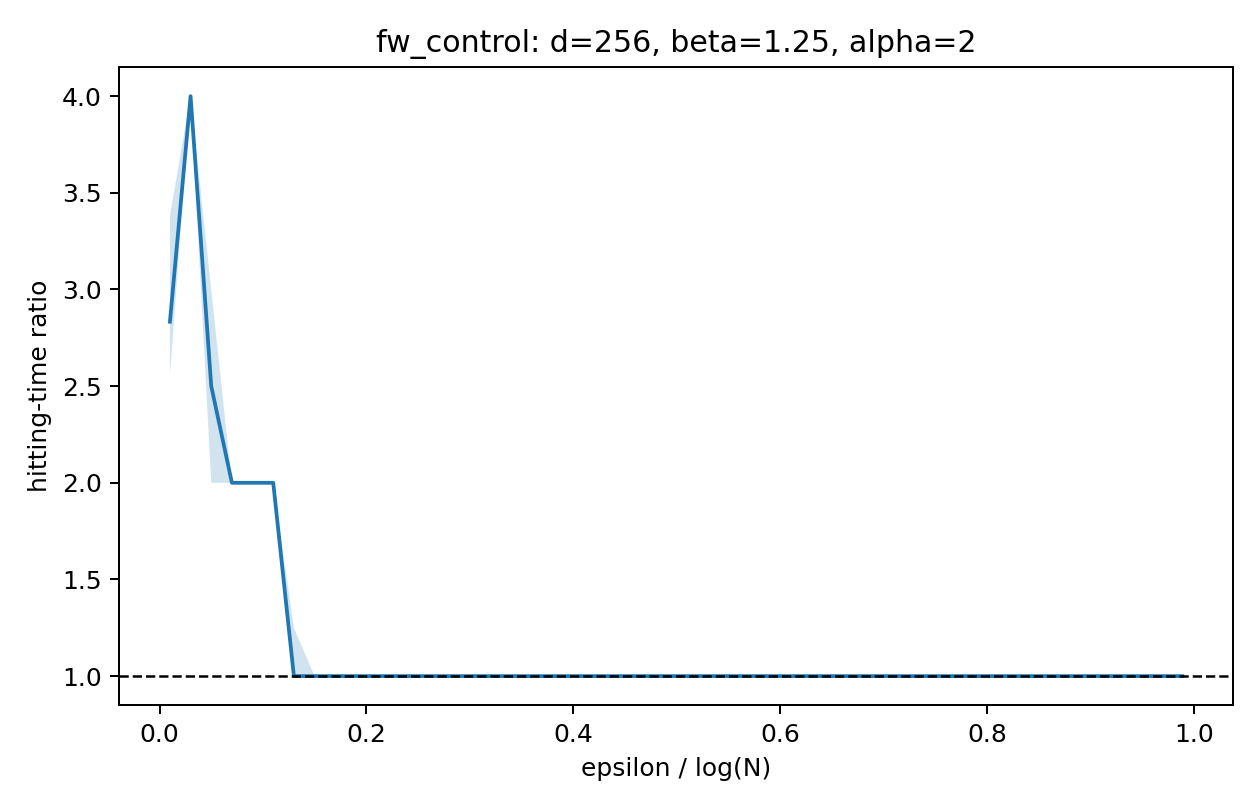
\includegraphics[width=\linewidth]{figures/ratio_curves/T_ratio_fw_control_d256_b1.25_a2.png}
\caption{$\alpha=2$}
\end{subfigure}%
\caption{Hitting-time ratio curves for FW-control, $\beta=1.25$, $d=256$, $N=1024$. Each panel is one value of $\alpha$. The solid line is the seed median and the shaded band is the interquartile range over three seeds.}
\label{fig:fw_control:T_ratio:b125}
\end{figure}






\subsubsection{$\beta=1.5$, $d=256$, $N=4096$}

The following three figures show the complete alpha sweep for this beta block: the best-AUC loss traces, the per-step hyperparameter envelope, and the hitting-time ratio. Reading them together is important: the loss curves show ordinary tuned trajectories, the envelope shows the best loss achievable at each iteration under the sweep, and the hitting-time ratio is the primary speed metric.

\begin{figure}[H]
\centering
\begin{subfigure}{0.22\textwidth}
\centering
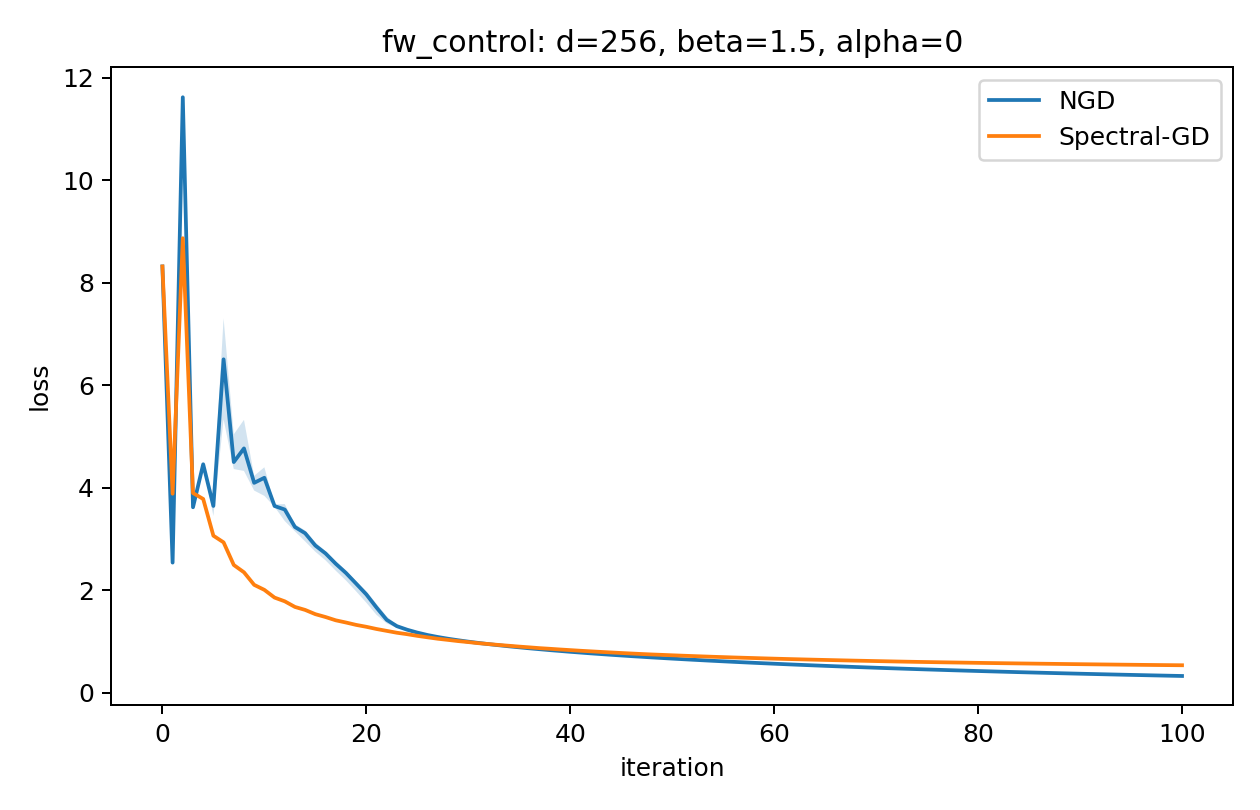
\includegraphics[width=\linewidth]{figures/loss_curves/fw_control_d256_b1.5_a0.png}
\caption{$\alpha=0$}
\end{subfigure}%
\hfill
\begin{subfigure}{0.22\textwidth}
\centering
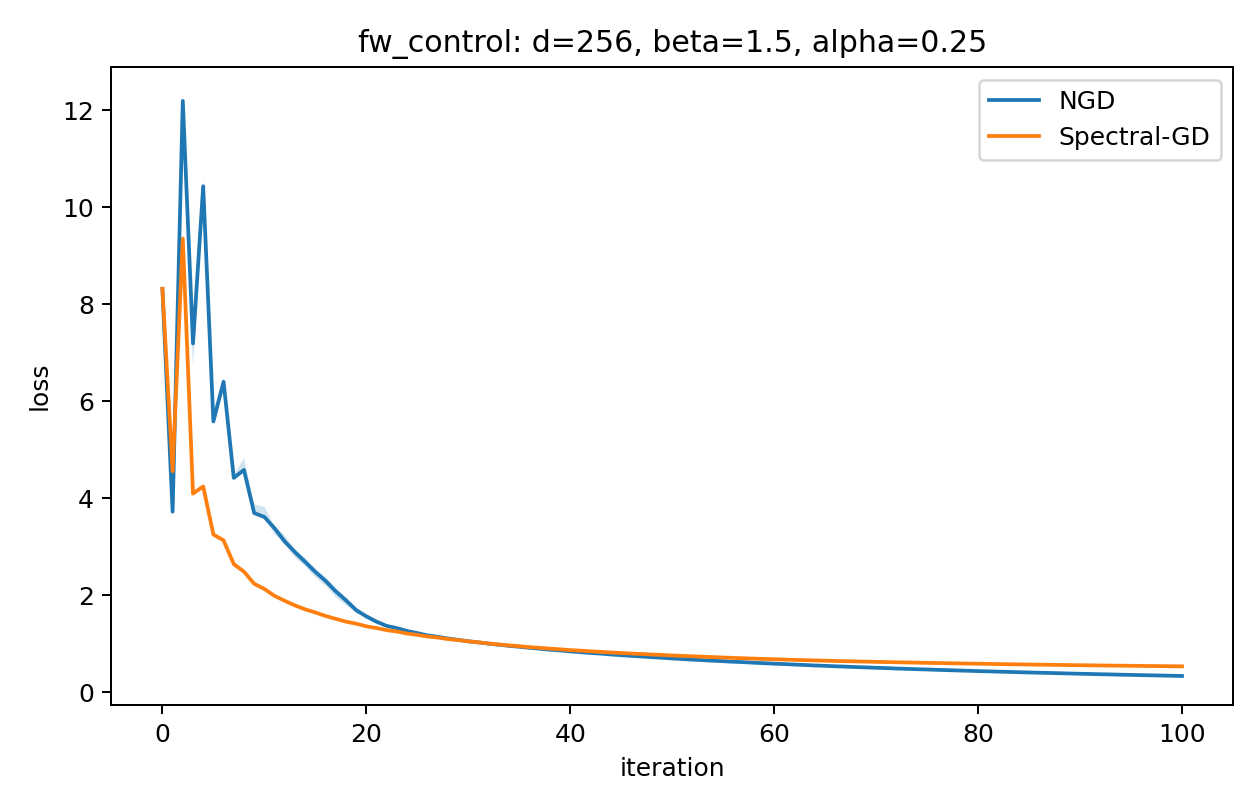
\includegraphics[width=\linewidth]{figures/loss_curves/fw_control_d256_b1.5_a0.25.png}
\caption{$\alpha=0.25$}
\end{subfigure}%
\hfill
\begin{subfigure}{0.22\textwidth}
\centering
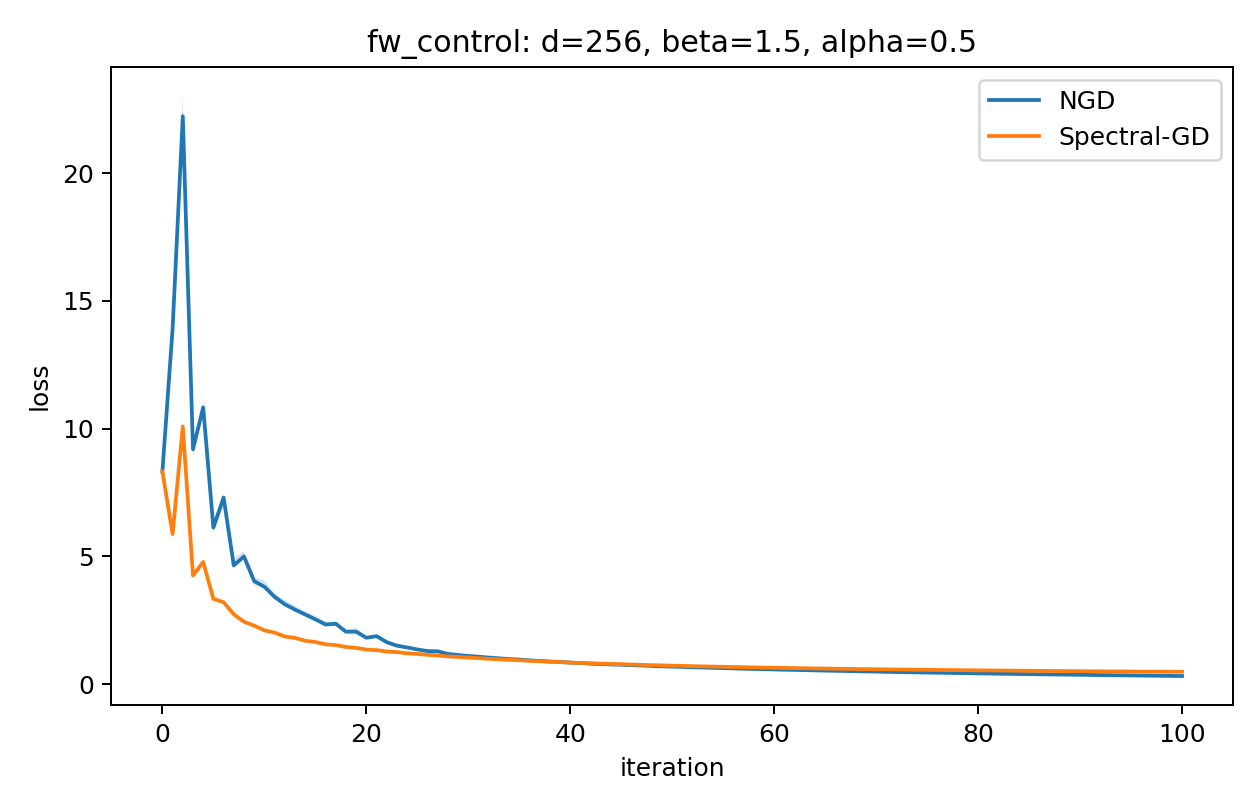
\includegraphics[width=\linewidth]{figures/loss_curves/fw_control_d256_b1.5_a0.5.png}
\caption{$\alpha=0.5$}
\end{subfigure}%
\hfill
\begin{subfigure}{0.22\textwidth}
\centering
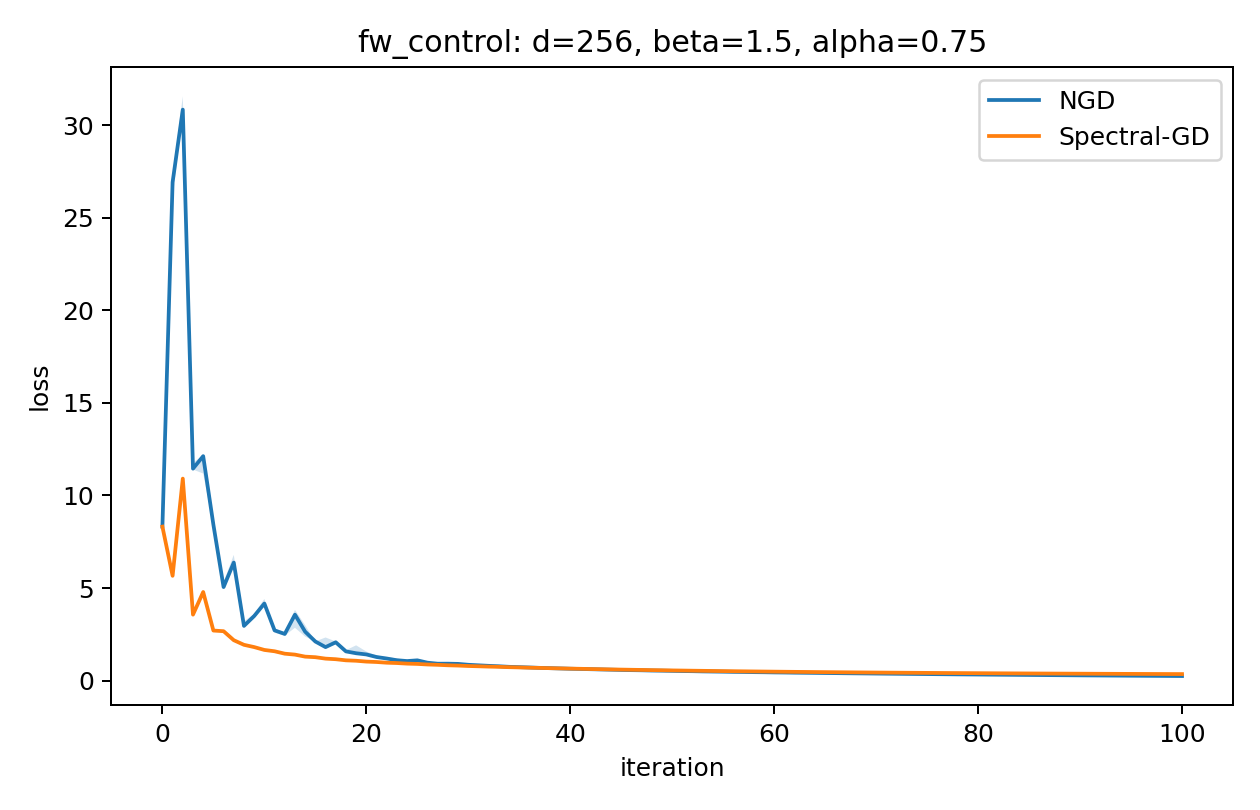
\includegraphics[width=\linewidth]{figures/loss_curves/fw_control_d256_b1.5_a0.75.png}
\caption{$\alpha=0.75$}
\end{subfigure}%
\par\smallskip
\begin{subfigure}{0.22\textwidth}
\centering
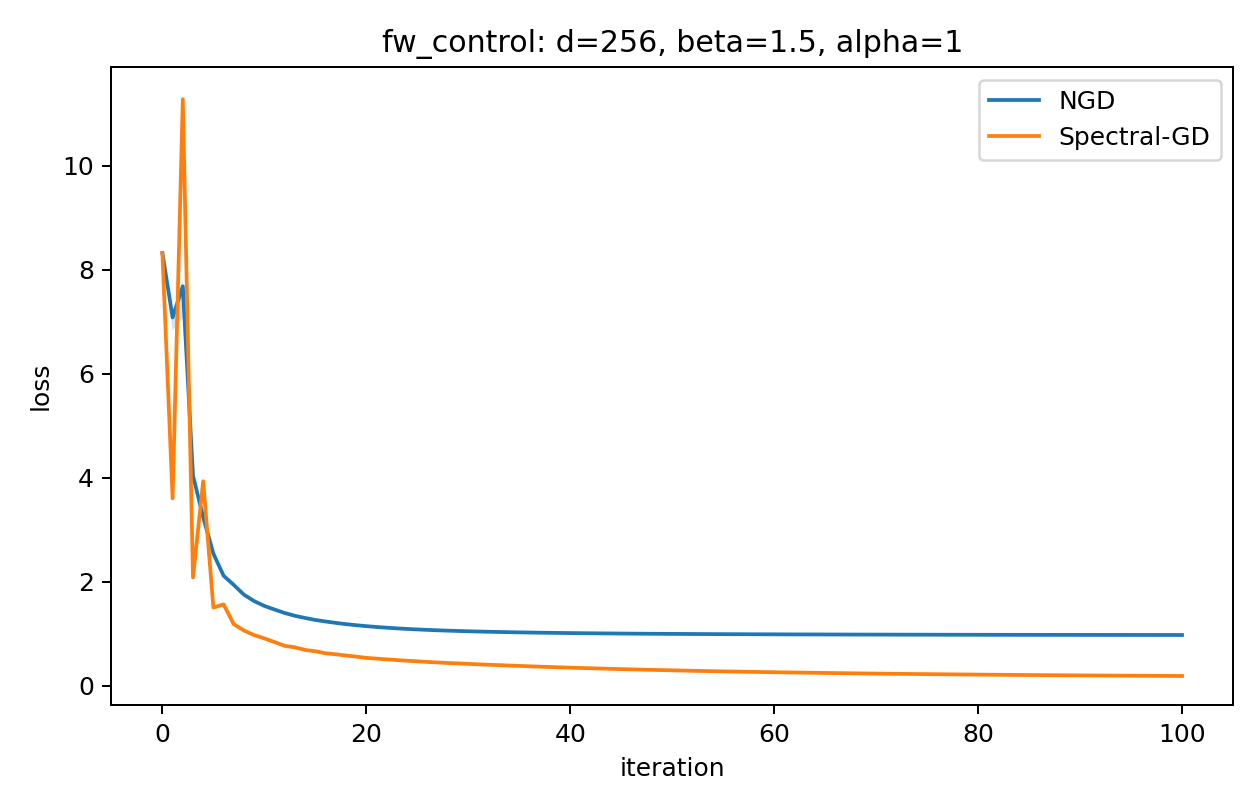
\includegraphics[width=\linewidth]{figures/loss_curves/fw_control_d256_b1.5_a1.png}
\caption{$\alpha=1$}
\end{subfigure}%
\hfill
\begin{subfigure}{0.22\textwidth}
\centering
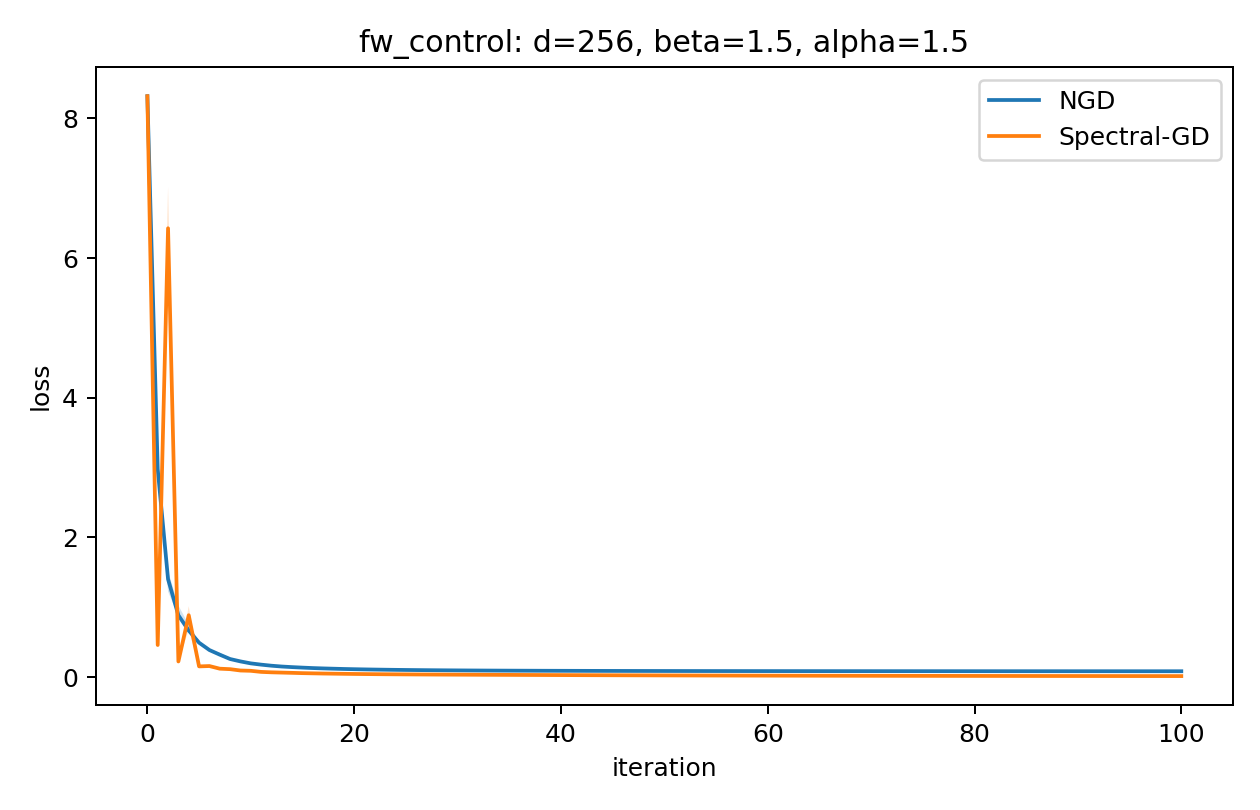
\includegraphics[width=\linewidth]{figures/loss_curves/fw_control_d256_b1.5_a1.5.png}
\caption{$\alpha=1.5$}
\end{subfigure}%
\hfill
\begin{subfigure}{0.22\textwidth}
\centering
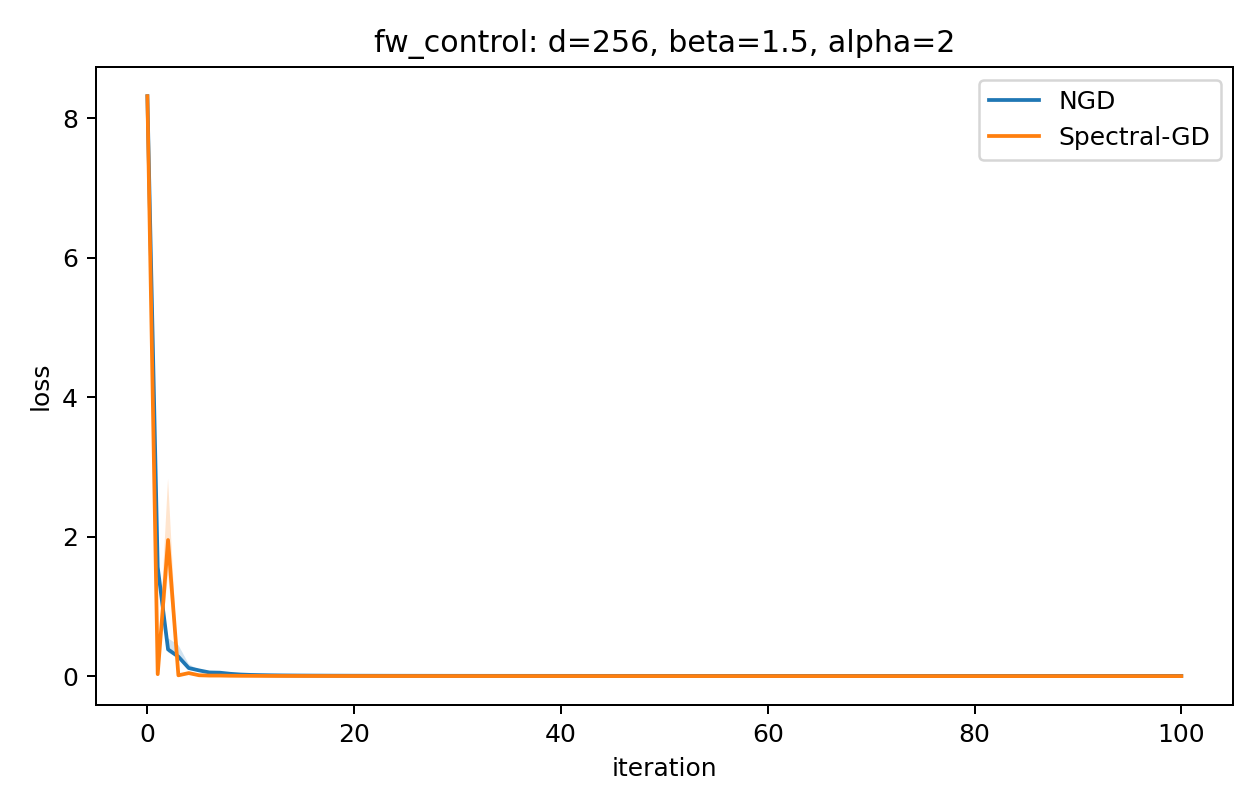
\includegraphics[width=\linewidth]{figures/loss_curves/fw_control_d256_b1.5_a2.png}
\caption{$\alpha=2$}
\end{subfigure}%
\caption{Best-auc loss curves for FW-control, $\beta=1.5$, $d=256$, $N=4096$. Each panel is one value of $\alpha$. The solid line is the seed median and the shaded band is the interquartile range over three seeds.}
\label{fig:fw_control:loss:b15}
\end{figure}


\begin{figure}[H]
\centering
\begin{subfigure}{0.22\textwidth}
\centering

\includegraphics[width=\linewidth]{figures/loss_envelope_curves/fw_control_d256_b1.5_a0.png}
\caption{$\alpha=0$}
\end{subfigure}%
\hfill
\begin{subfigure}{0.22\textwidth}
\centering

\includegraphics[width=\linewidth]{figures/loss_envelope_curves/fw_control_d256_b1.5_a0.25.png}
\caption{$\alpha=0.25$}
\end{subfigure}%
\hfill
\begin{subfigure}{0.22\textwidth}
\centering

\includegraphics[width=\linewidth]{figures/loss_envelope_curves/fw_control_d256_b1.5_a0.5.png}
\caption{$\alpha=0.5$}
\end{subfigure}%
\hfill
\begin{subfigure}{0.22\textwidth}
\centering

\includegraphics[width=\linewidth]{figures/loss_envelope_curves/fw_control_d256_b1.5_a0.75.png}
\caption{$\alpha=0.75$}
\end{subfigure}%
\par\smallskip
\begin{subfigure}{0.22\textwidth}
\centering

\includegraphics[width=\linewidth]{figures/loss_envelope_curves/fw_control_d256_b1.5_a1.png}
\caption{$\alpha=1$}
\end{subfigure}%
\hfill
\begin{subfigure}{0.22\textwidth}
\centering

\includegraphics[width=\linewidth]{figures/loss_envelope_curves/fw_control_d256_b1.5_a1.5.png}
\caption{$\alpha=1.5$}
\end{subfigure}%
\hfill
\begin{subfigure}{0.22\textwidth}
\centering

\includegraphics[width=\linewidth]{figures/loss_envelope_curves/fw_control_d256_b1.5_a2.png}
\caption{$\alpha=2$}
\end{subfigure}%
\caption{Loss envelope curves for FW-control, $\beta=1.5$, $d=256$, $N=4096$. Each panel is one value of $\alpha$. The solid line is the seed median and the shaded band is the interquartile range over three seeds.}
\label{fig:fw_control:envelope:b15}
\end{figure}


\begin{figure}[H]
\centering
\begin{subfigure}{0.22\textwidth}
\centering
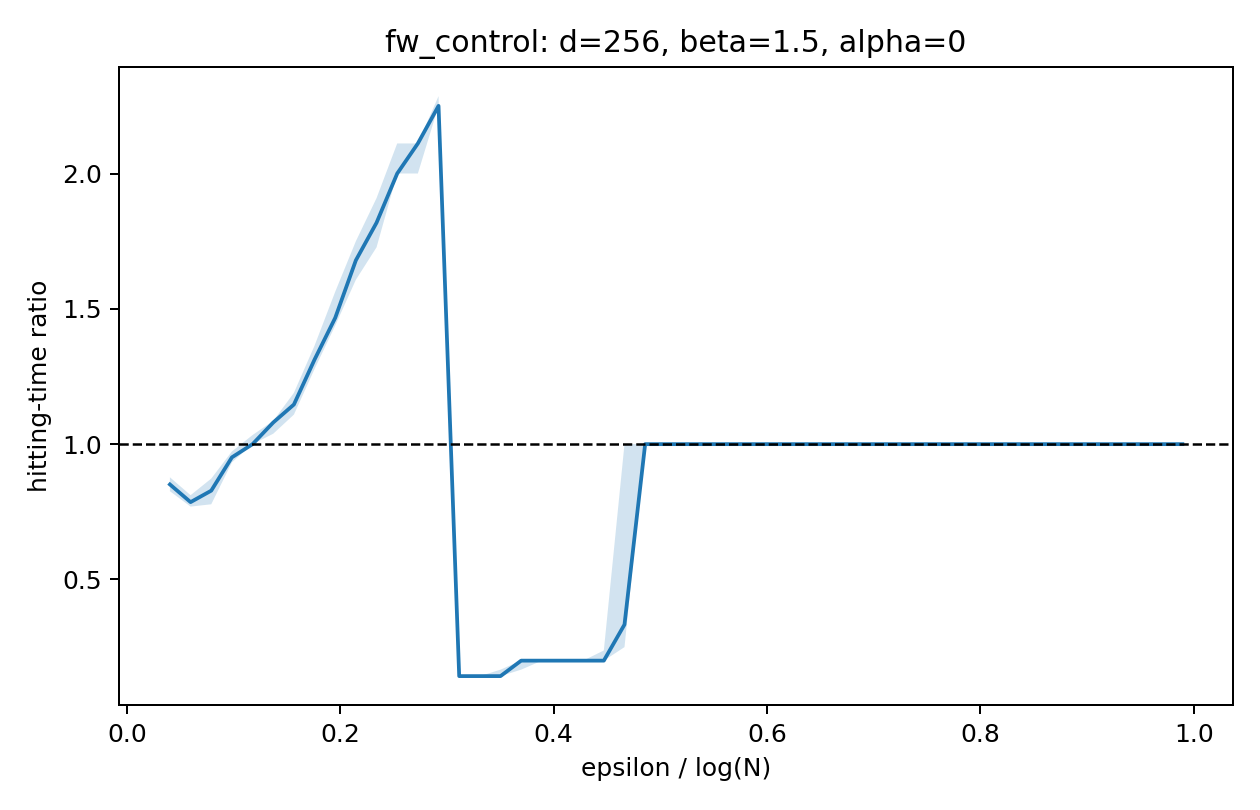
\includegraphics[width=\linewidth]{figures/ratio_curves/T_ratio_fw_control_d256_b1.5_a0.png}
\caption{$\alpha=0$}
\end{subfigure}%
\hfill
\begin{subfigure}{0.22\textwidth}
\centering
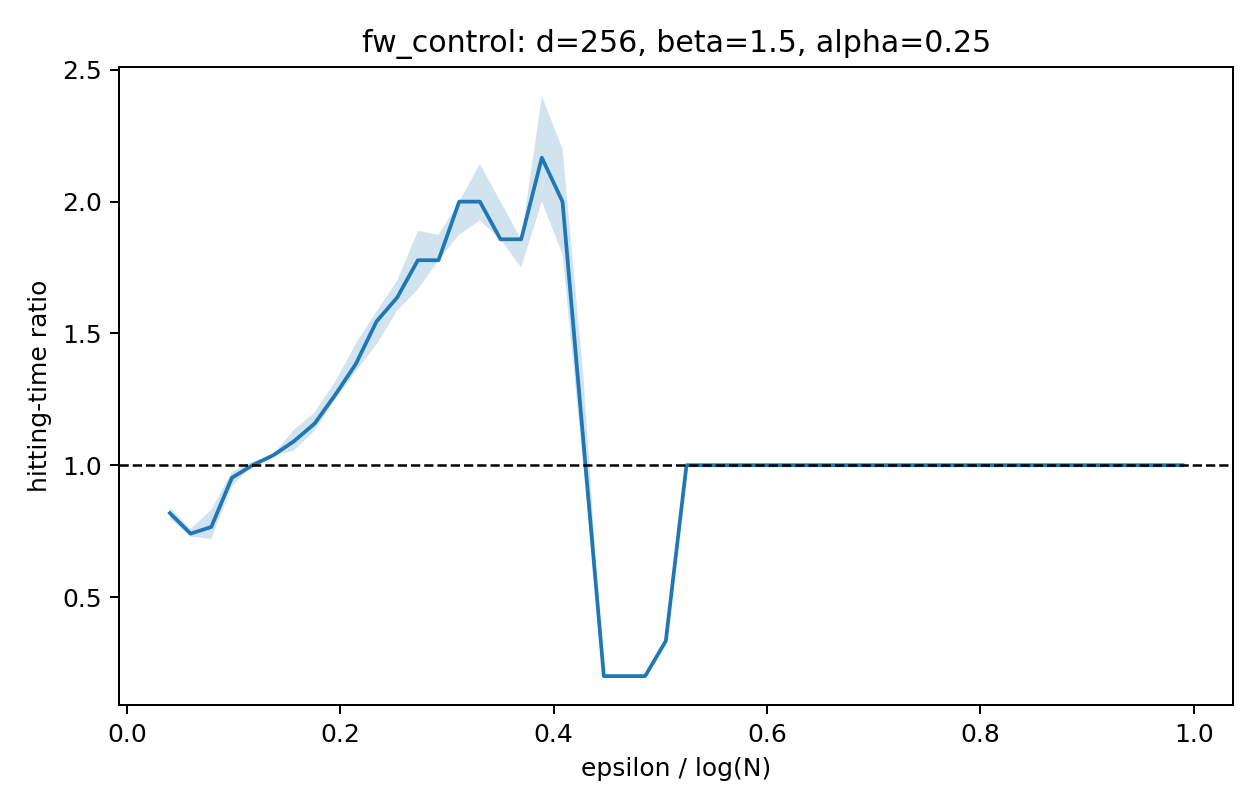
\includegraphics[width=\linewidth]{figures/ratio_curves/T_ratio_fw_control_d256_b1.5_a0.25.png}
\caption{$\alpha=0.25$}
\end{subfigure}%
\hfill
\begin{subfigure}{0.22\textwidth}
\centering
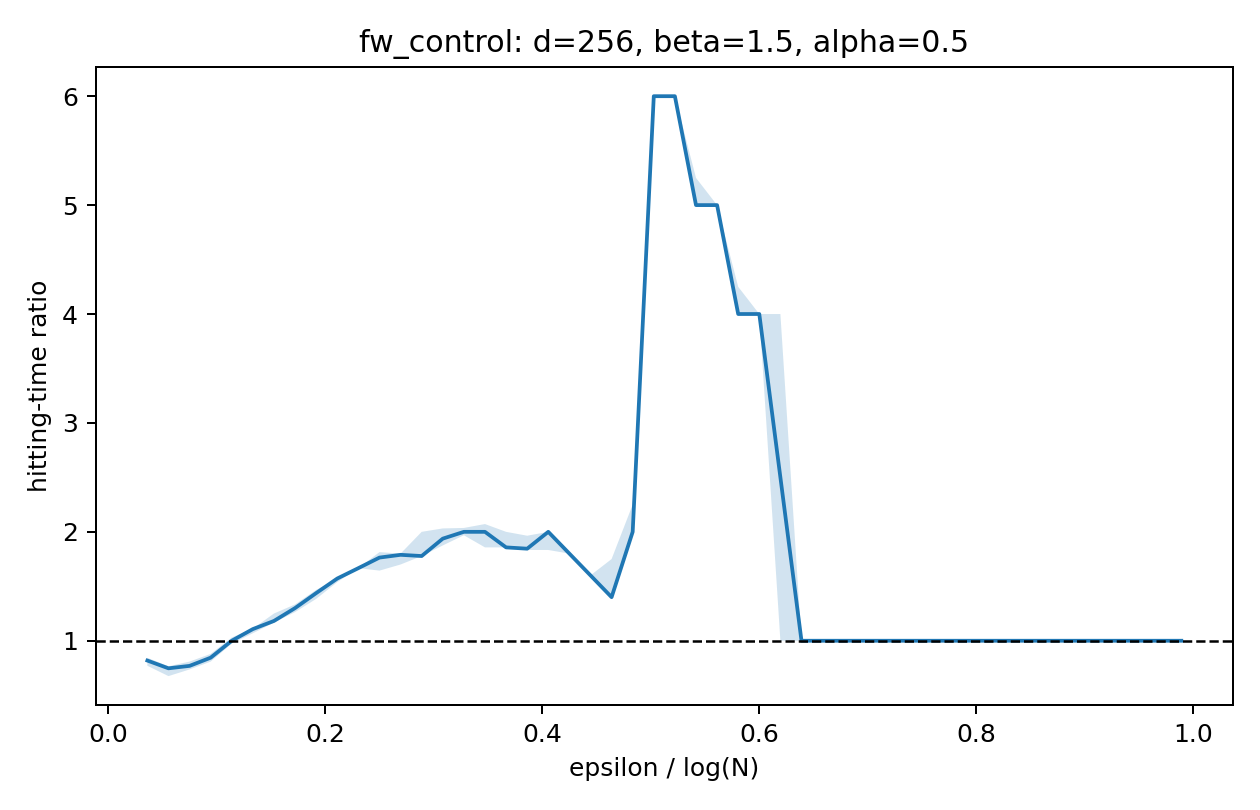
\includegraphics[width=\linewidth]{figures/ratio_curves/T_ratio_fw_control_d256_b1.5_a0.5.png}
\caption{$\alpha=0.5$}
\end{subfigure}%
\hfill
\begin{subfigure}{0.22\textwidth}
\centering
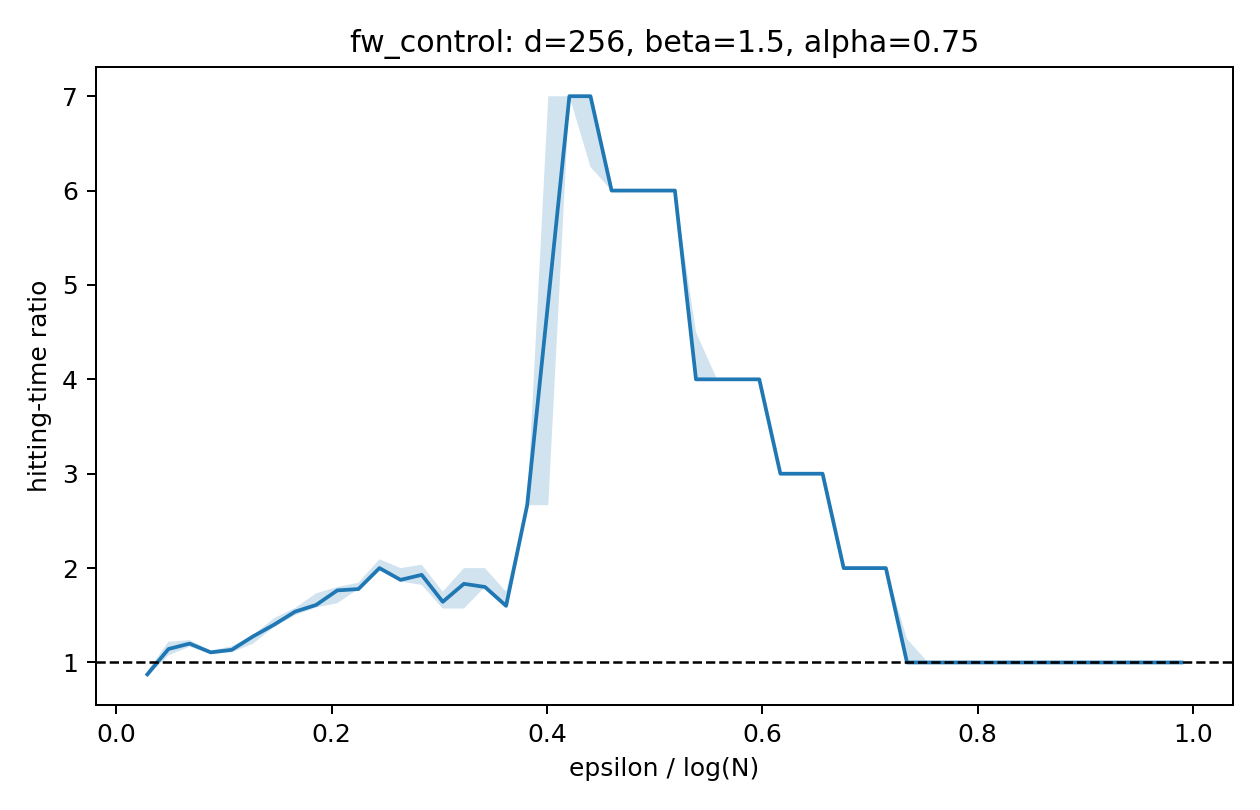
\includegraphics[width=\linewidth]{figures/ratio_curves/T_ratio_fw_control_d256_b1.5_a0.75.png}
\caption{$\alpha=0.75$}
\end{subfigure}%
\par\smallskip
\begin{subfigure}{0.22\textwidth}
\centering
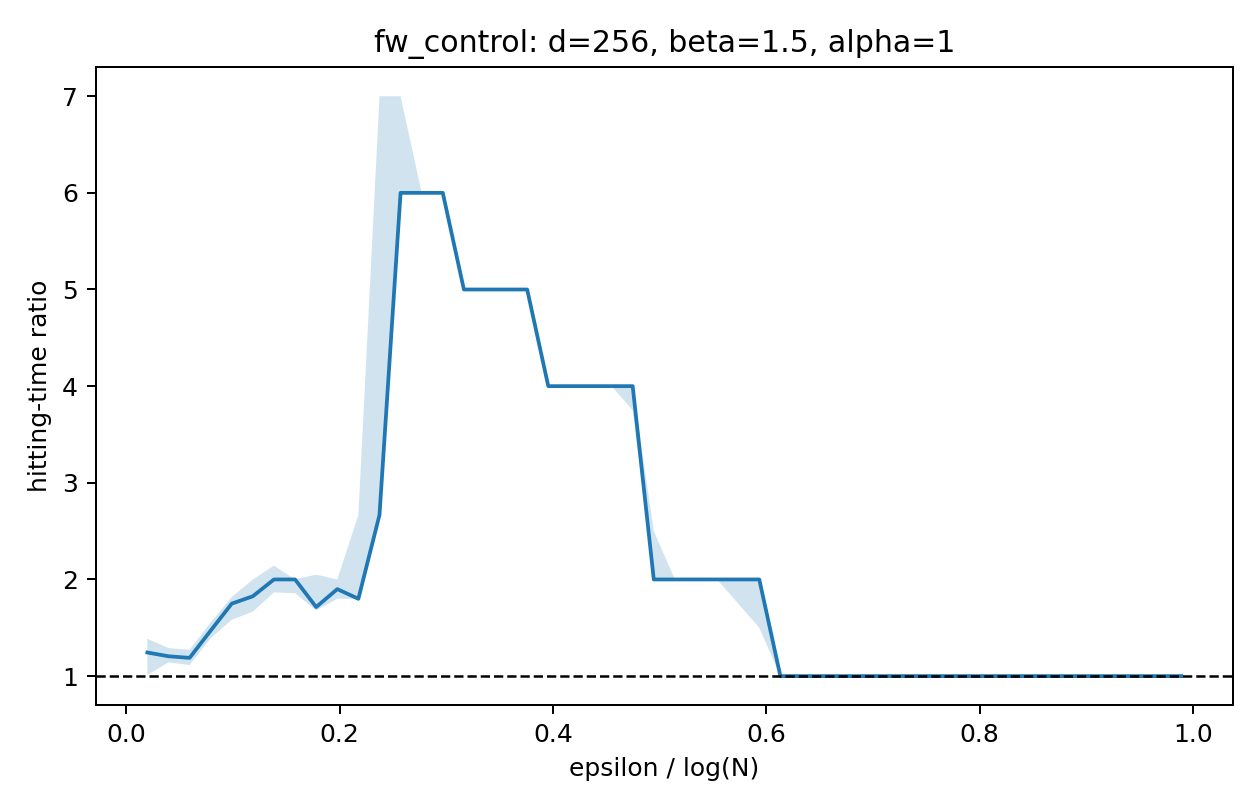
\includegraphics[width=\linewidth]{figures/ratio_curves/T_ratio_fw_control_d256_b1.5_a1.png}
\caption{$\alpha=1$}
\end{subfigure}%
\hfill
\begin{subfigure}{0.22\textwidth}
\centering
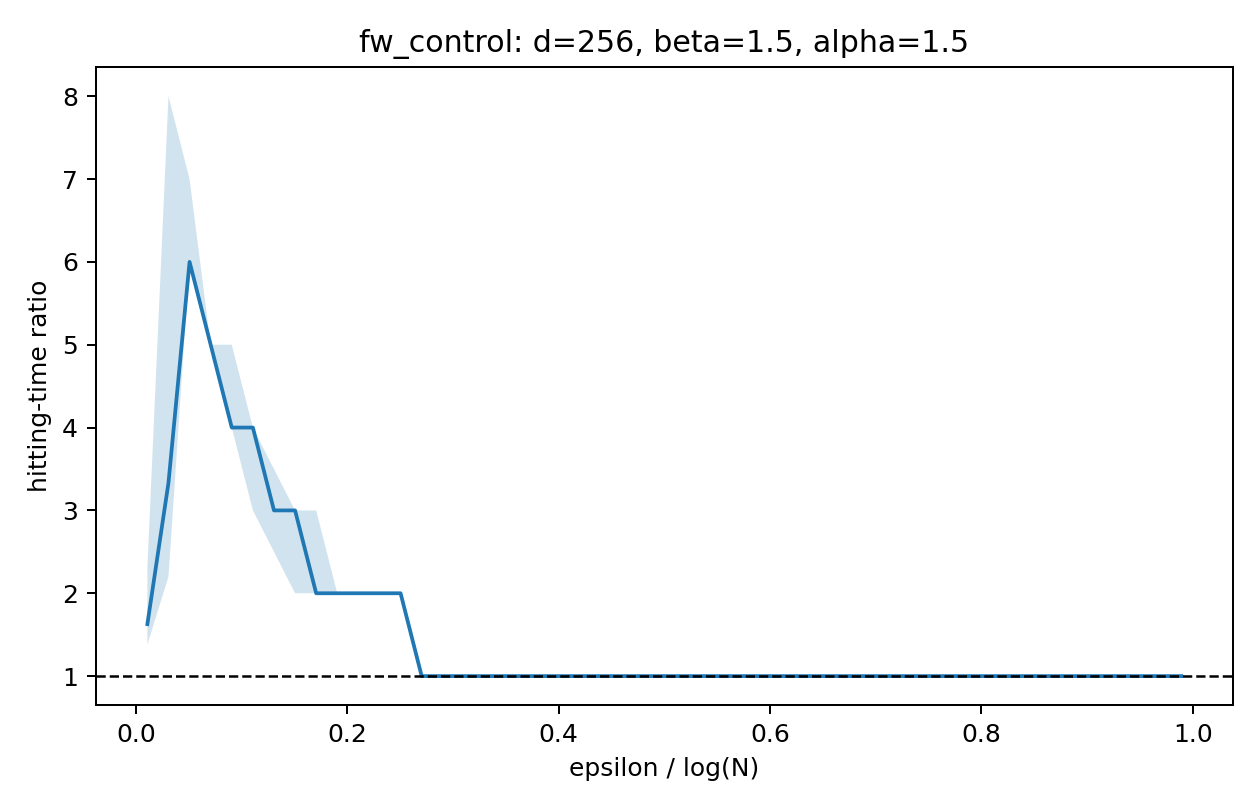
\includegraphics[width=\linewidth]{figures/ratio_curves/T_ratio_fw_control_d256_b1.5_a1.5.png}
\caption{$\alpha=1.5$}
\end{subfigure}%
\hfill
\begin{subfigure}{0.22\textwidth}
\centering
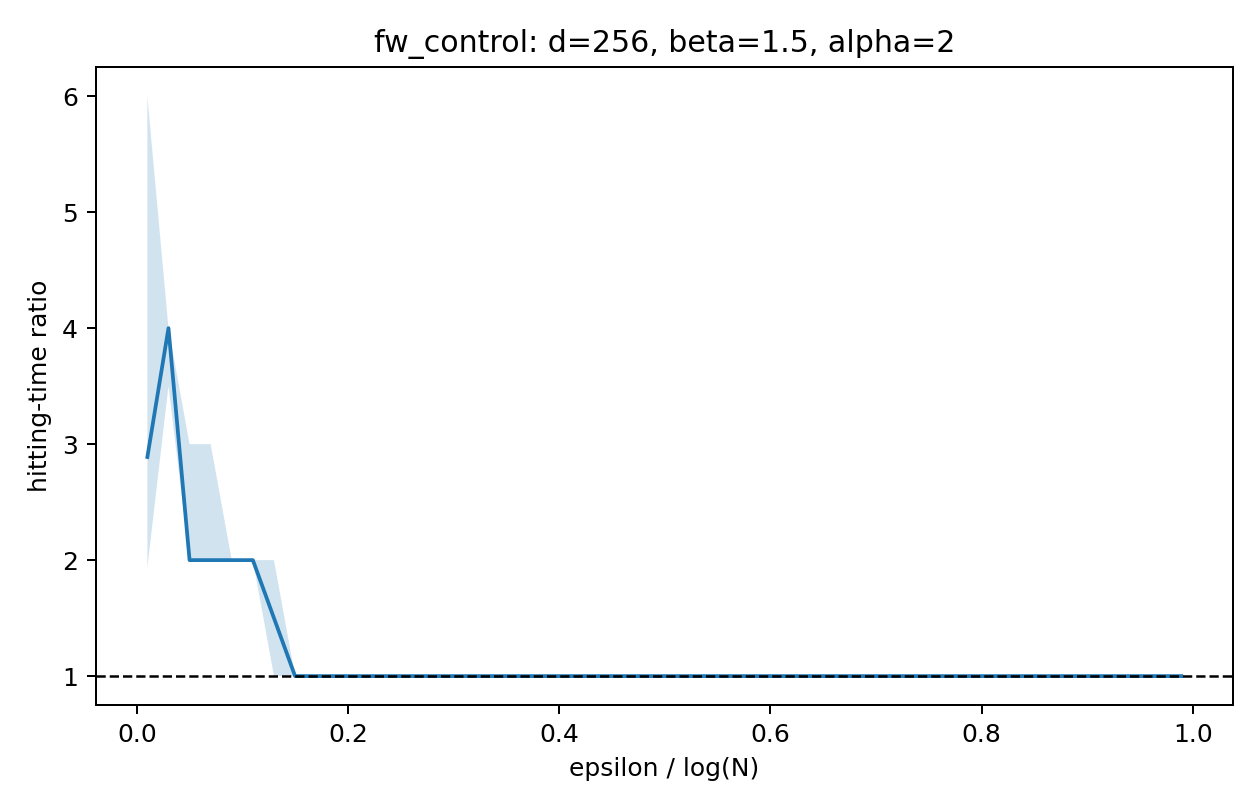
\includegraphics[width=\linewidth]{figures/ratio_curves/T_ratio_fw_control_d256_b1.5_a2.png}
\caption{$\alpha=2$}
\end{subfigure}%
\caption{Hitting-time ratio curves for FW-control, $\beta=1.5$, $d=256$, $N=4096$. Each panel is one value of $\alpha$. The solid line is the seed median and the shaded band is the interquartile range over three seeds.}
\label{fig:fw_control:T_ratio:b15}
\end{figure}






\subsubsection{$\beta_{\rm eff}=2.101845$, $d=80$, $N=10000$}

The following three figures show the complete alpha sweep for this beta block: the best-AUC loss traces, the per-step hyperparameter envelope, and the hitting-time ratio. Reading them together is important: the loss curves show ordinary tuned trajectories, the envelope shows the best loss achievable at each iteration under the sweep, and the hitting-time ratio is the primary speed metric.

\begin{figure}[H]
\centering
\begin{subfigure}{0.22\textwidth}
\centering
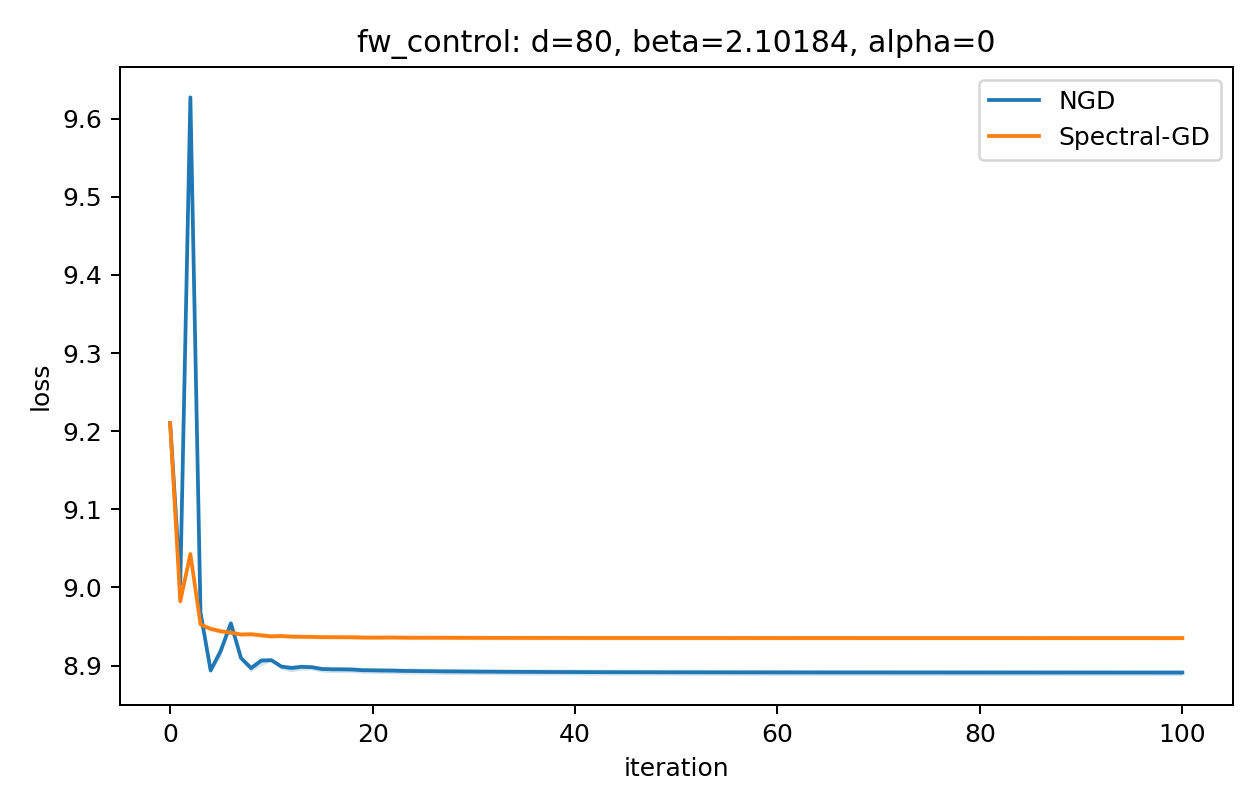
\includegraphics[width=\linewidth]{figures/loss_curves/fw_control_d80_b2.10184_a0.png}
\caption{$\alpha=0$}
\end{subfigure}%
\hfill
\begin{subfigure}{0.22\textwidth}
\centering
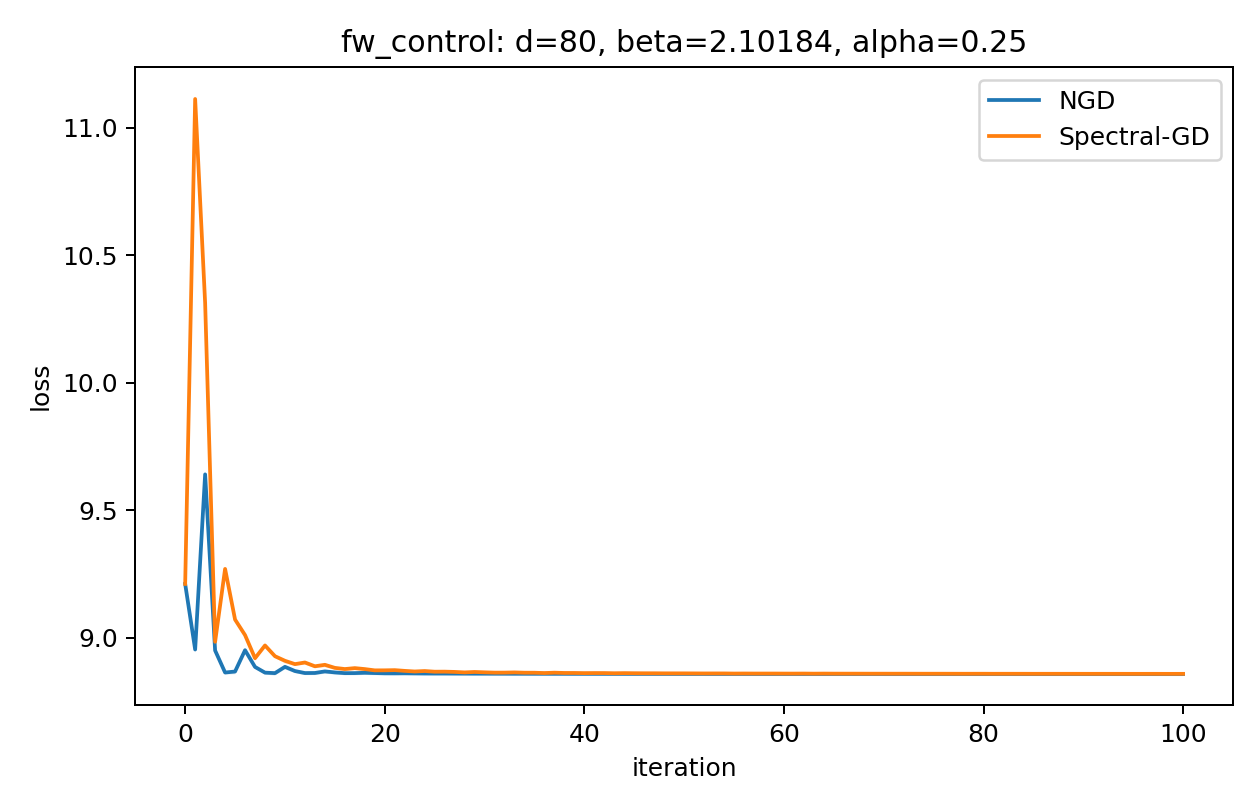
\includegraphics[width=\linewidth]{figures/loss_curves/fw_control_d80_b2.10184_a0.25.png}
\caption{$\alpha=0.25$}
\end{subfigure}%
\hfill
\begin{subfigure}{0.22\textwidth}
\centering
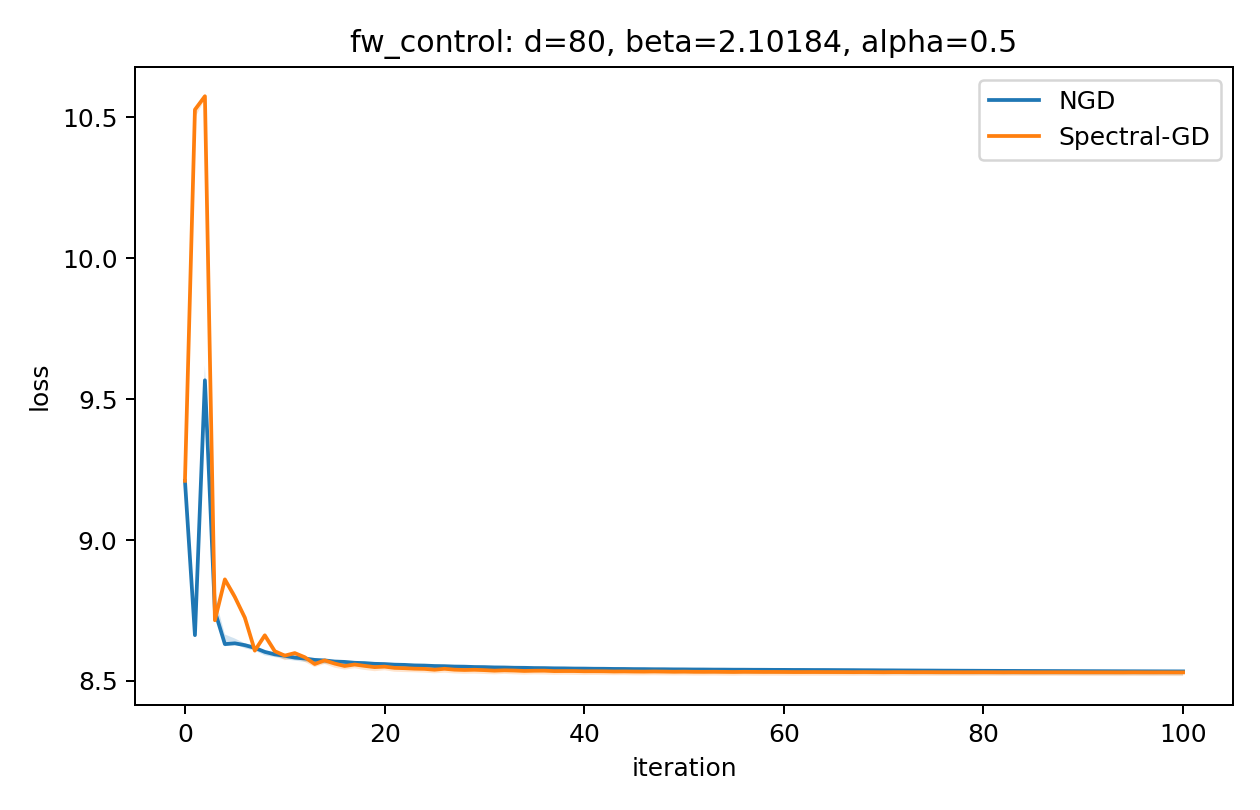
\includegraphics[width=\linewidth]{figures/loss_curves/fw_control_d80_b2.10184_a0.5.png}
\caption{$\alpha=0.5$}
\end{subfigure}%
\hfill
\begin{subfigure}{0.22\textwidth}
\centering
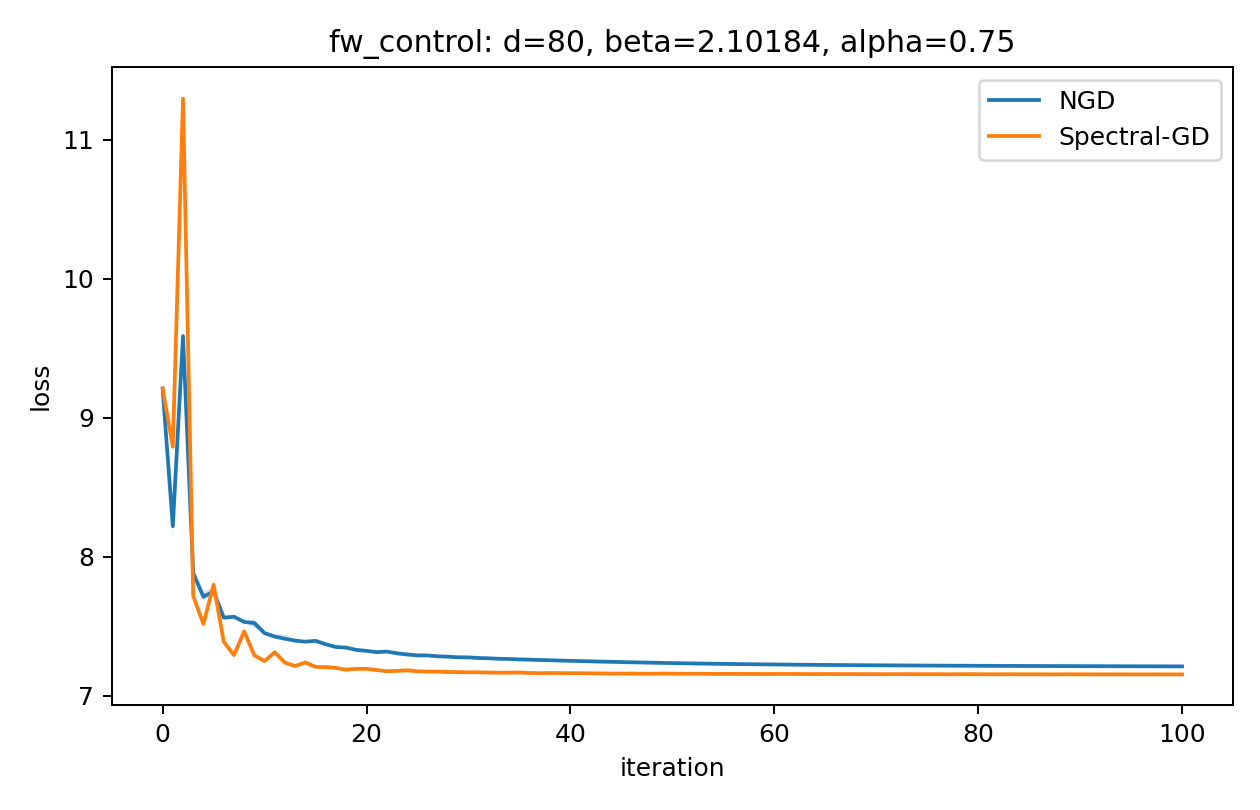
\includegraphics[width=\linewidth]{figures/loss_curves/fw_control_d80_b2.10184_a0.75.png}
\caption{$\alpha=0.75$}
\end{subfigure}%
\par\smallskip
\begin{subfigure}{0.22\textwidth}
\centering
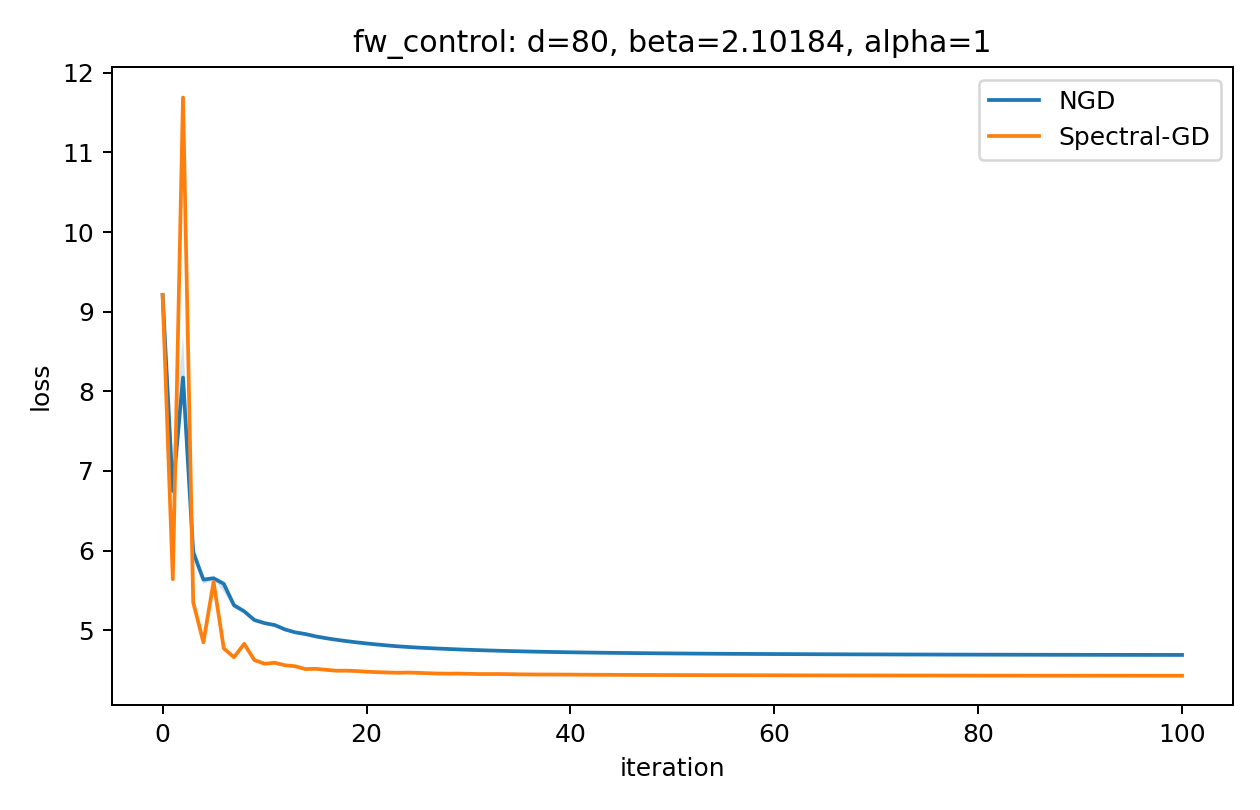
\includegraphics[width=\linewidth]{figures/loss_curves/fw_control_d80_b2.10184_a1.png}
\caption{$\alpha=1$}
\end{subfigure}%
\hfill
\begin{subfigure}{0.22\textwidth}
\centering
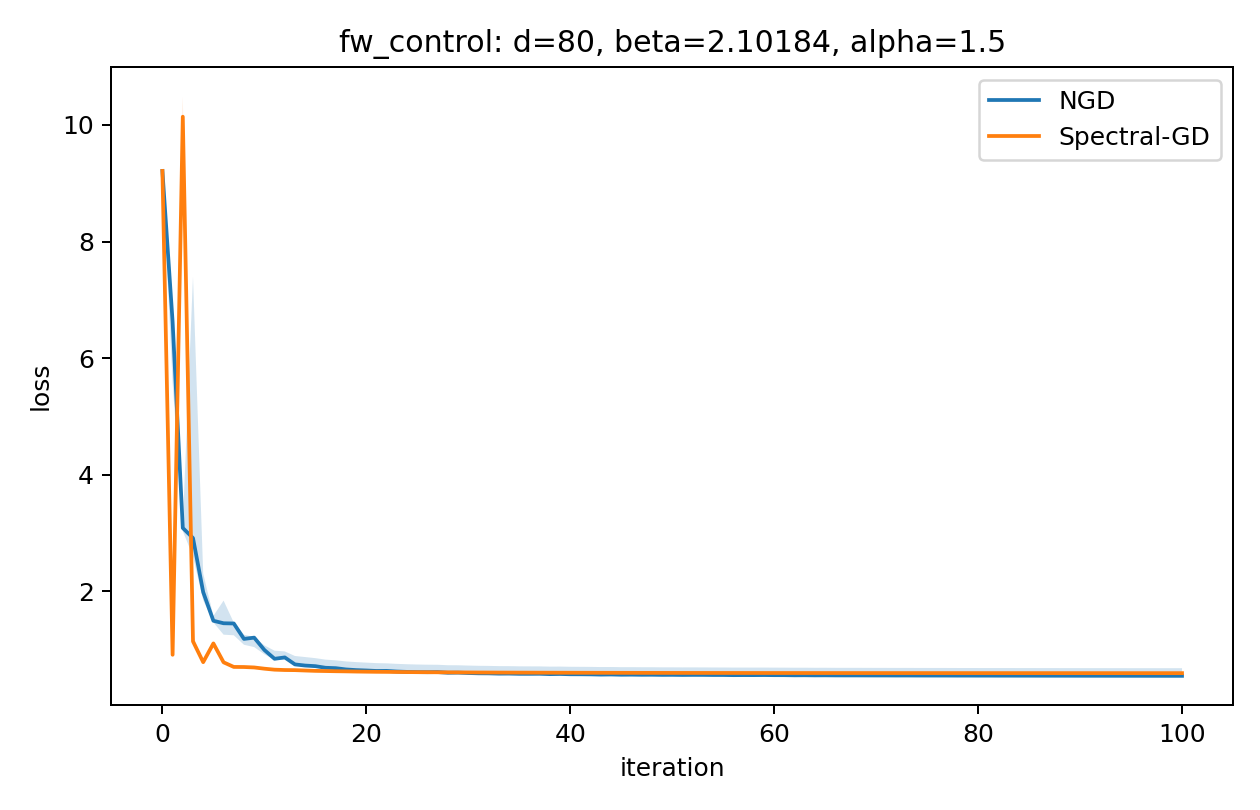
\includegraphics[width=\linewidth]{figures/loss_curves/fw_control_d80_b2.10184_a1.5.png}
\caption{$\alpha=1.5$}
\end{subfigure}%
\hfill
\begin{subfigure}{0.22\textwidth}
\centering
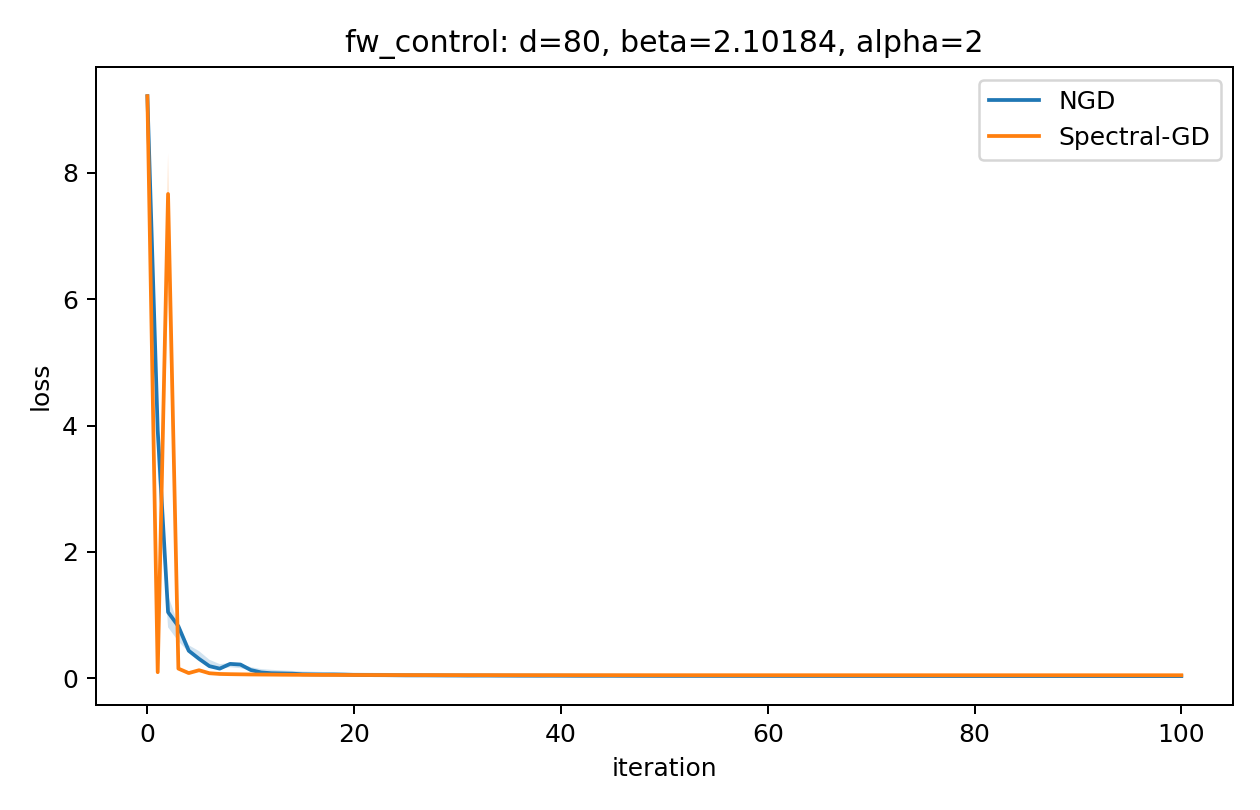
\includegraphics[width=\linewidth]{figures/loss_curves/fw_control_d80_b2.10184_a2.png}
\caption{$\alpha=2$}
\end{subfigure}%
\caption{Best-auc loss curves for FW-control, $\beta_{\rm eff}=2.101845$, $d=80$, $N=10000$. Each panel is one value of $\alpha$. The solid line is the seed median and the shaded band is the interquartile range over three seeds.}
\label{fig:fw_control:loss:beff210}
\end{figure}


\begin{figure}[H]
\centering
\begin{subfigure}{0.22\textwidth}
\centering

\includegraphics[width=\linewidth]{figures/loss_envelope_curves/fw_control_d80_b2.10184_a0.png}
\caption{$\alpha=0$}
\end{subfigure}%
\hfill
\begin{subfigure}{0.22\textwidth}
\centering

\includegraphics[width=\linewidth]{figures/loss_envelope_curves/fw_control_d80_b2.10184_a0.25.png}
\caption{$\alpha=0.25$}
\end{subfigure}%
\hfill
\begin{subfigure}{0.22\textwidth}
\centering

\includegraphics[width=\linewidth]{figures/loss_envelope_curves/fw_control_d80_b2.10184_a0.5.png}
\caption{$\alpha=0.5$}
\end{subfigure}%
\hfill
\begin{subfigure}{0.22\textwidth}
\centering

\includegraphics[width=\linewidth]{figures/loss_envelope_curves/fw_control_d80_b2.10184_a0.75.png}
\caption{$\alpha=0.75$}
\end{subfigure}%
\par\smallskip
\begin{subfigure}{0.22\textwidth}
\centering

\includegraphics[width=\linewidth]{figures/loss_envelope_curves/fw_control_d80_b2.10184_a1.png}
\caption{$\alpha=1$}
\end{subfigure}%
\hfill
\begin{subfigure}{0.22\textwidth}
\centering

\includegraphics[width=\linewidth]{figures/loss_envelope_curves/fw_control_d80_b2.10184_a1.5.png}
\caption{$\alpha=1.5$}
\end{subfigure}%
\hfill
\begin{subfigure}{0.22\textwidth}
\centering

\includegraphics[width=\linewidth]{figures/loss_envelope_curves/fw_control_d80_b2.10184_a2.png}
\caption{$\alpha=2$}
\end{subfigure}%
\caption{Loss envelope curves for FW-control, $\beta_{\rm eff}=2.101845$, $d=80$, $N=10000$. Each panel is one value of $\alpha$. The solid line is the seed median and the shaded band is the interquartile range over three seeds.}
\label{fig:fw_control:envelope:beff210}
\end{figure}


\begin{figure}[H]
\centering
\begin{subfigure}{0.22\textwidth}
\centering
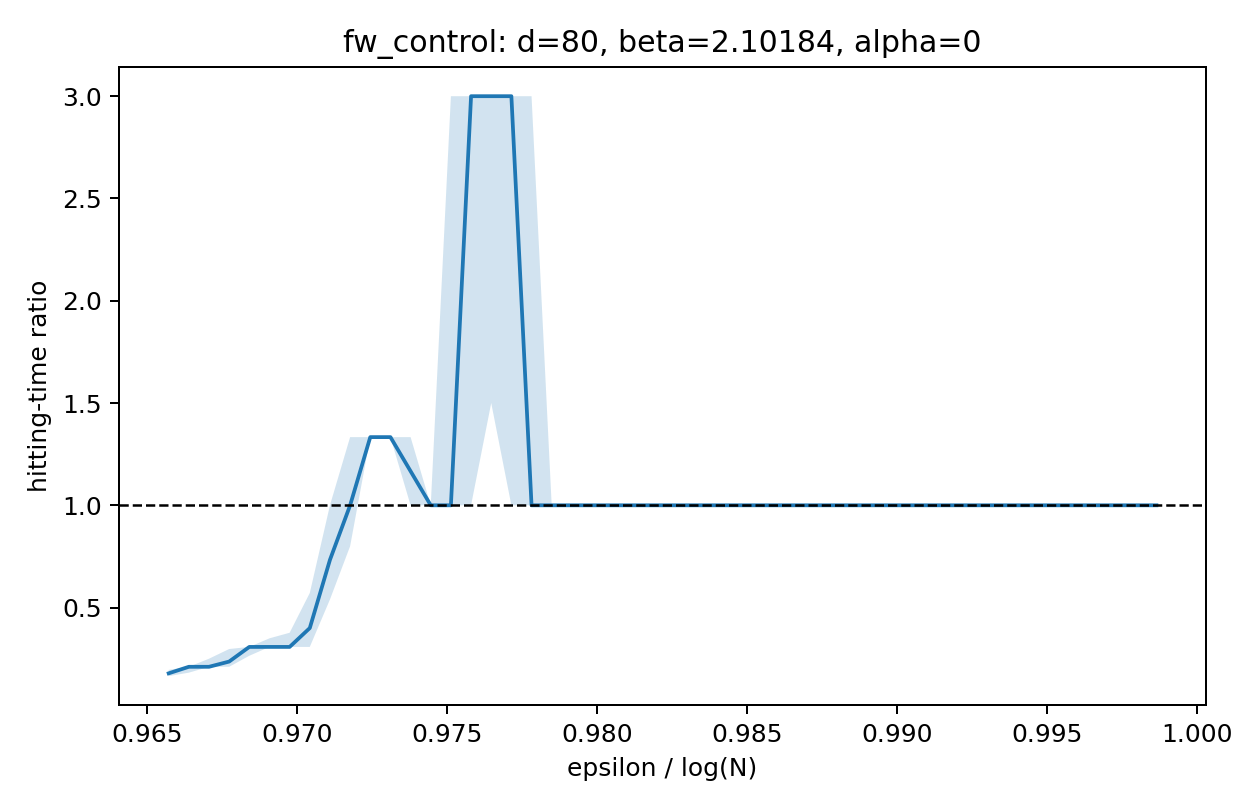
\includegraphics[width=\linewidth]{figures/ratio_curves/T_ratio_fw_control_d80_b2.10184_a0.png}
\caption{$\alpha=0$}
\end{subfigure}%
\hfill
\begin{subfigure}{0.22\textwidth}
\centering
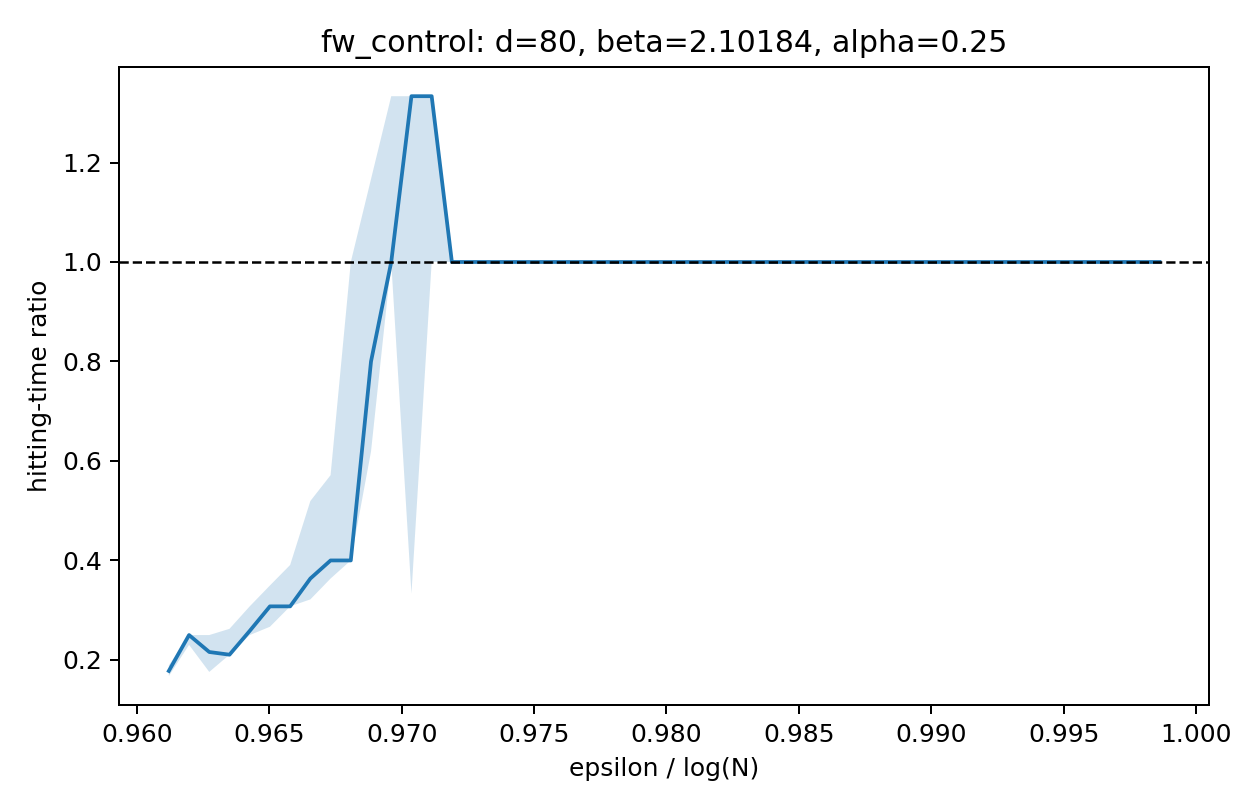
\includegraphics[width=\linewidth]{figures/ratio_curves/T_ratio_fw_control_d80_b2.10184_a0.25.png}
\caption{$\alpha=0.25$}
\end{subfigure}%
\hfill
\begin{subfigure}{0.22\textwidth}
\centering
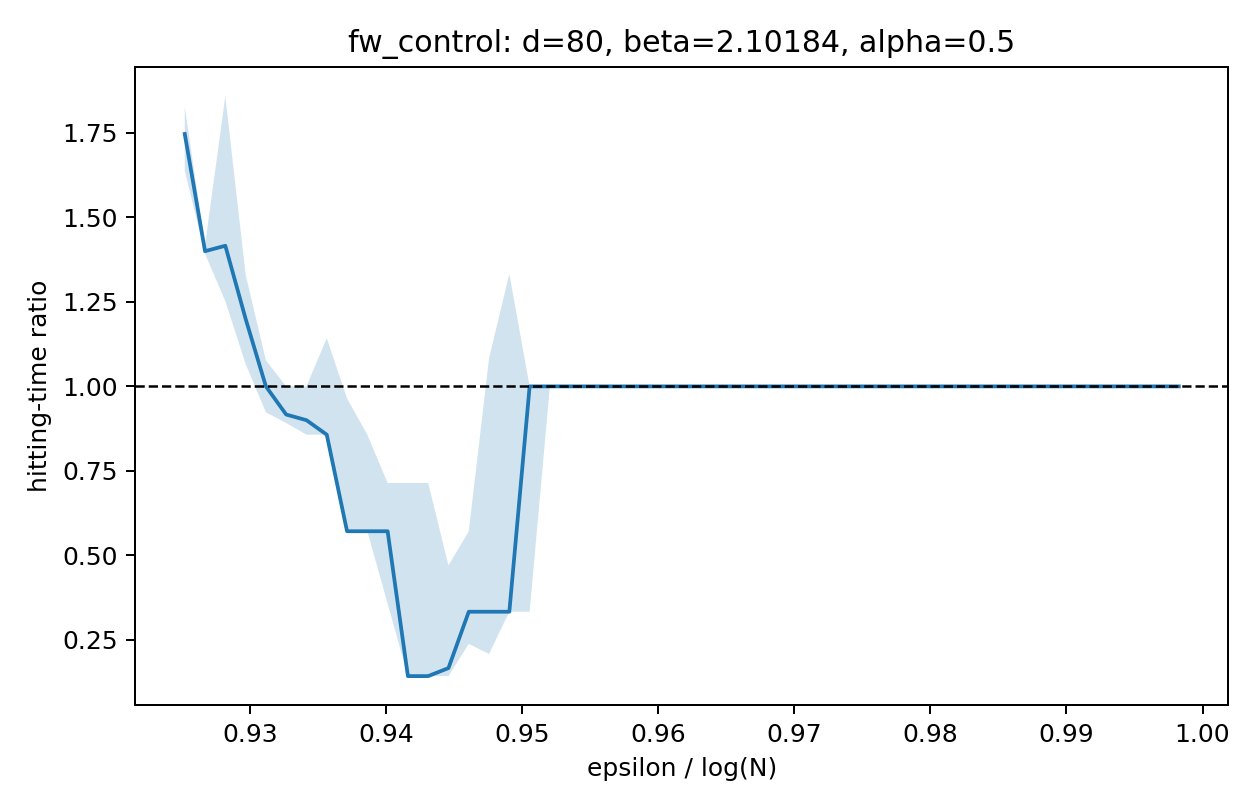
\includegraphics[width=\linewidth]{figures/ratio_curves/T_ratio_fw_control_d80_b2.10184_a0.5.png}
\caption{$\alpha=0.5$}
\end{subfigure}%
\hfill
\begin{subfigure}{0.22\textwidth}
\centering
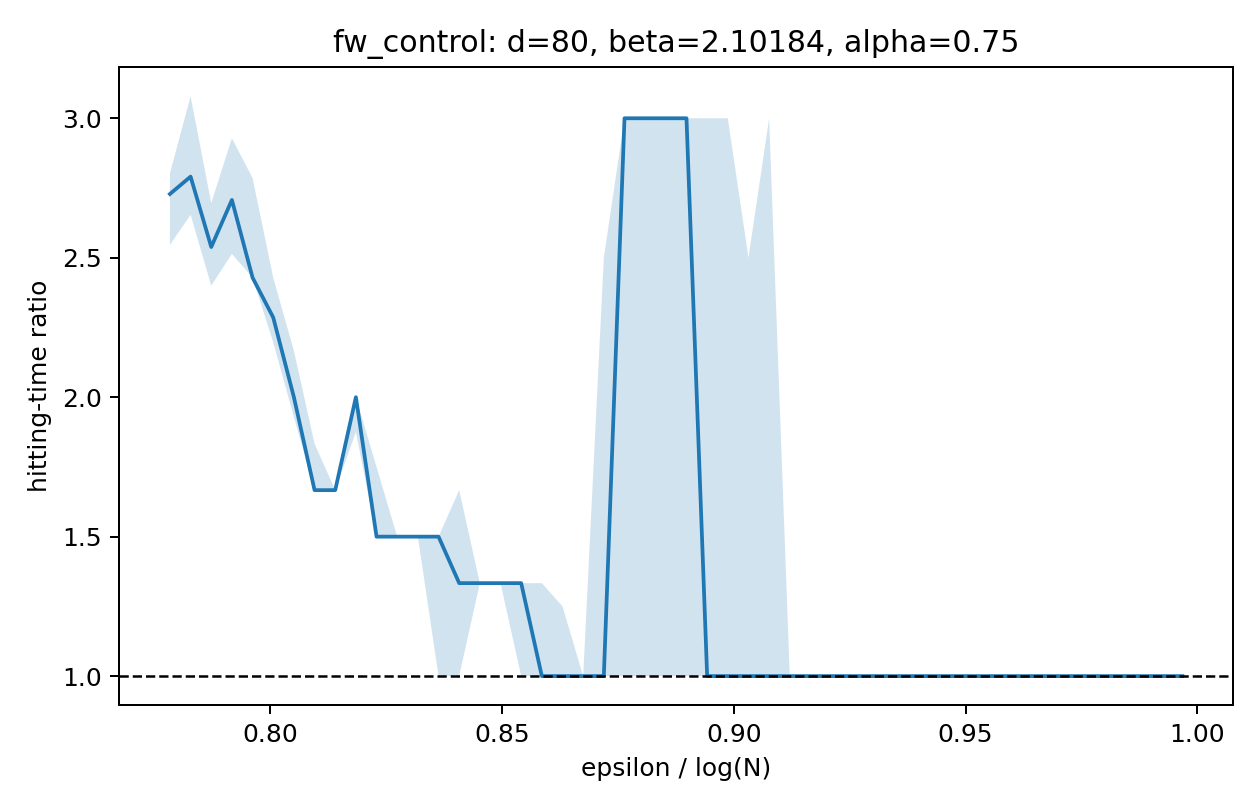
\includegraphics[width=\linewidth]{figures/ratio_curves/T_ratio_fw_control_d80_b2.10184_a0.75.png}
\caption{$\alpha=0.75$}
\end{subfigure}%
\par\smallskip
\begin{subfigure}{0.22\textwidth}
\centering
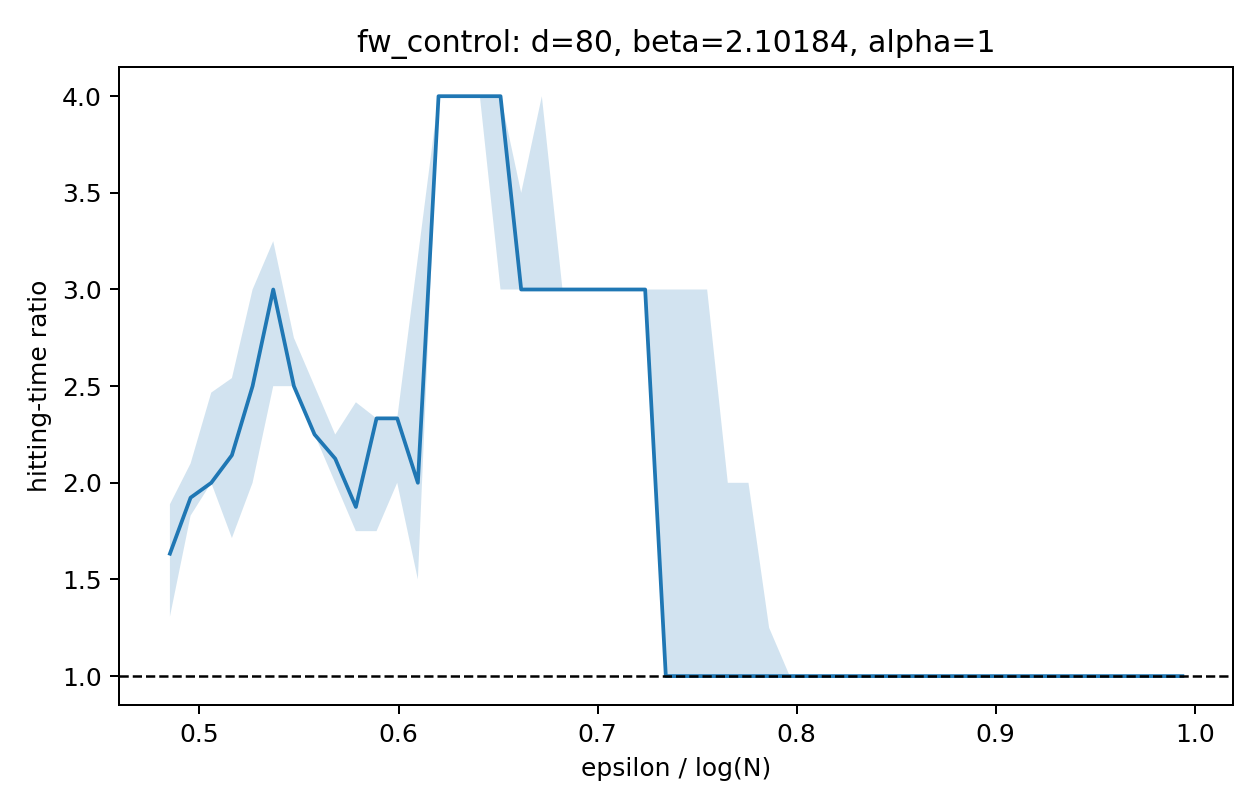
\includegraphics[width=\linewidth]{figures/ratio_curves/T_ratio_fw_control_d80_b2.10184_a1.png}
\caption{$\alpha=1$}
\end{subfigure}%
\hfill
\begin{subfigure}{0.22\textwidth}
\centering
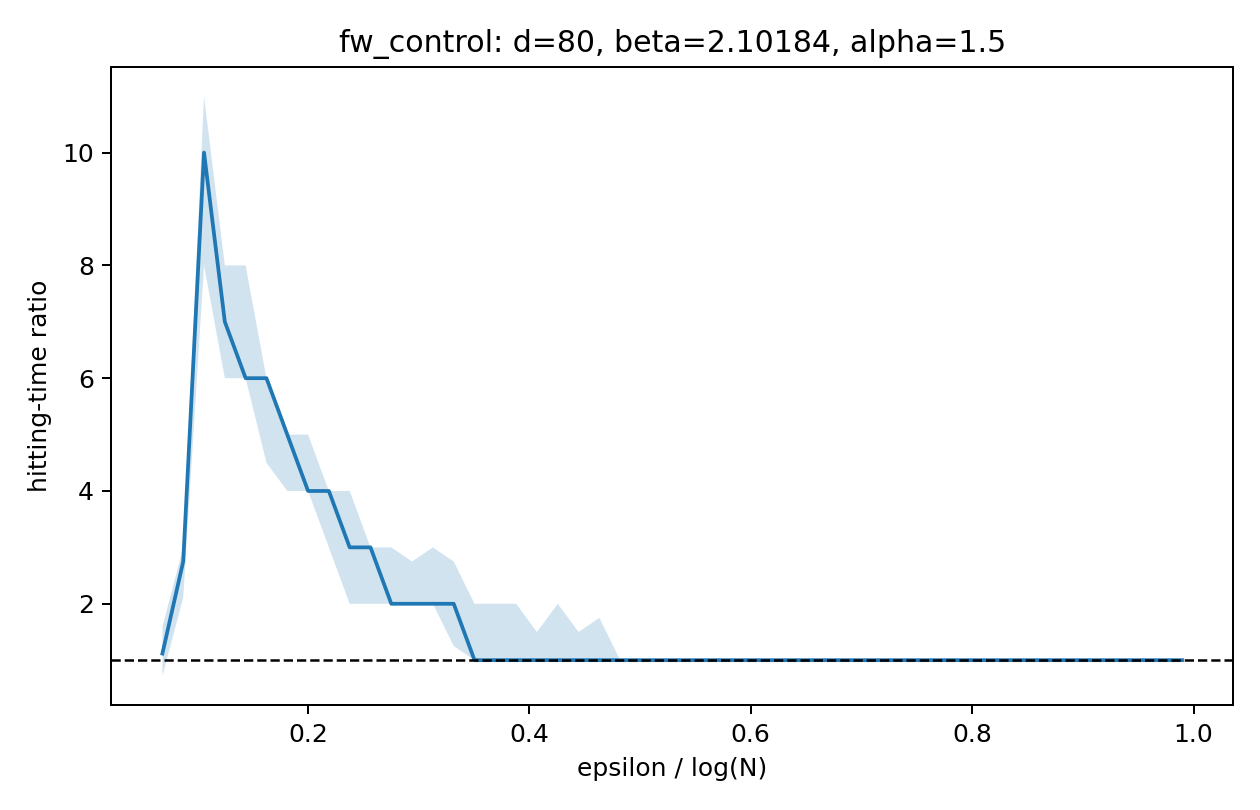
\includegraphics[width=\linewidth]{figures/ratio_curves/T_ratio_fw_control_d80_b2.10184_a1.5.png}
\caption{$\alpha=1.5$}
\end{subfigure}%
\hfill
\begin{subfigure}{0.22\textwidth}
\centering
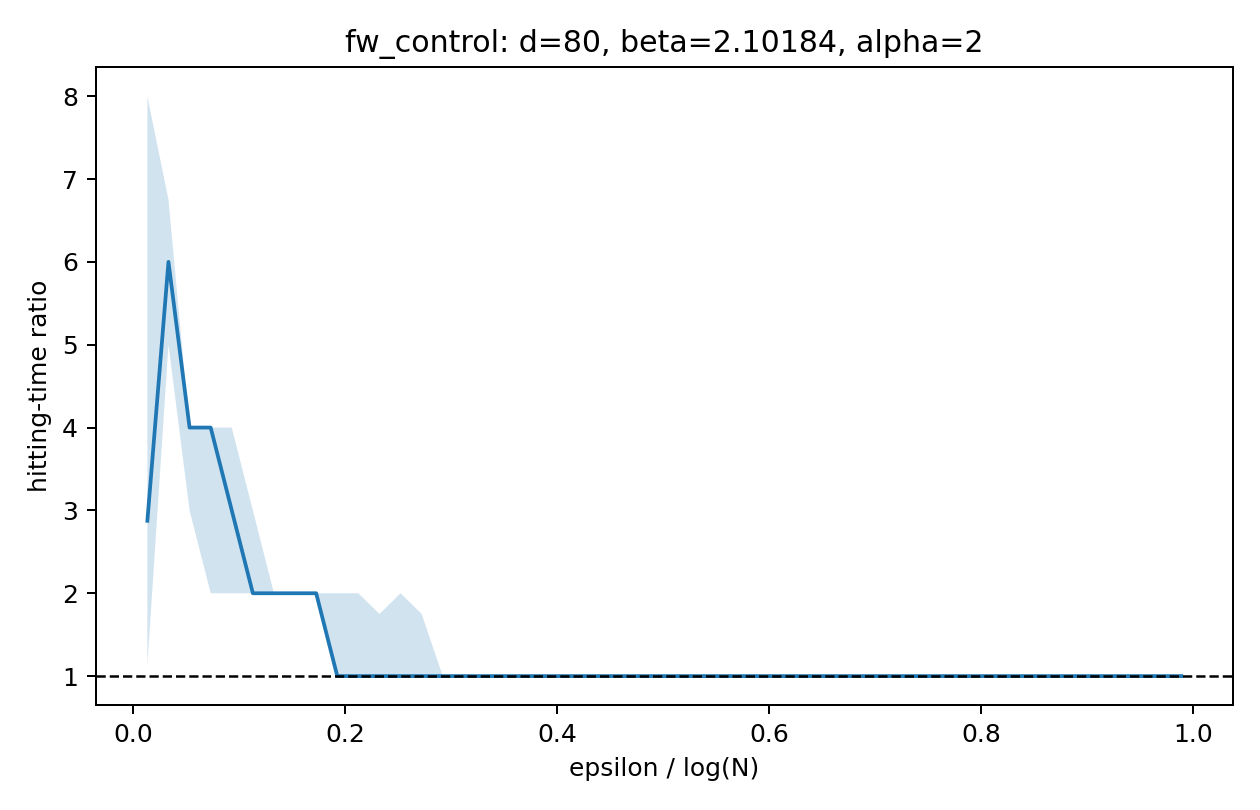
\includegraphics[width=\linewidth]{figures/ratio_curves/T_ratio_fw_control_d80_b2.10184_a2.png}
\caption{$\alpha=2$}
\end{subfigure}%
\caption{Hitting-time ratio curves for FW-control, $\beta_{\rm eff}=2.101845$, $d=80$, $N=10000$. Each panel is one value of $\alpha$. The solid line is the seed median and the shaded band is the interquartile range over three seeds.}
\label{fig:fw_control:T_ratio:beff210}
\end{figure}



\subsection{Complete pooled trajectory-radius proxy grids}

The following figures add the pooled trajectory-radius proxy diagnostic for every beta block. Each panel plots
\[
  Q_{\rm traj}(\eps;s)=R_{\F}^{\rm traj}(\eps;s)/R_{\op}^{\rm traj}(\eps;s)
\]
against $\eps/\log N$. The radius proxy pools all recorded realistic-training and FW-control trajectory points within the same regime and seed before taking the minimum recorded Frobenius and operator radii at each target loss.

\begin{figure}[H]
\centering
\begin{subfigure}{0.22\textwidth}
\centering
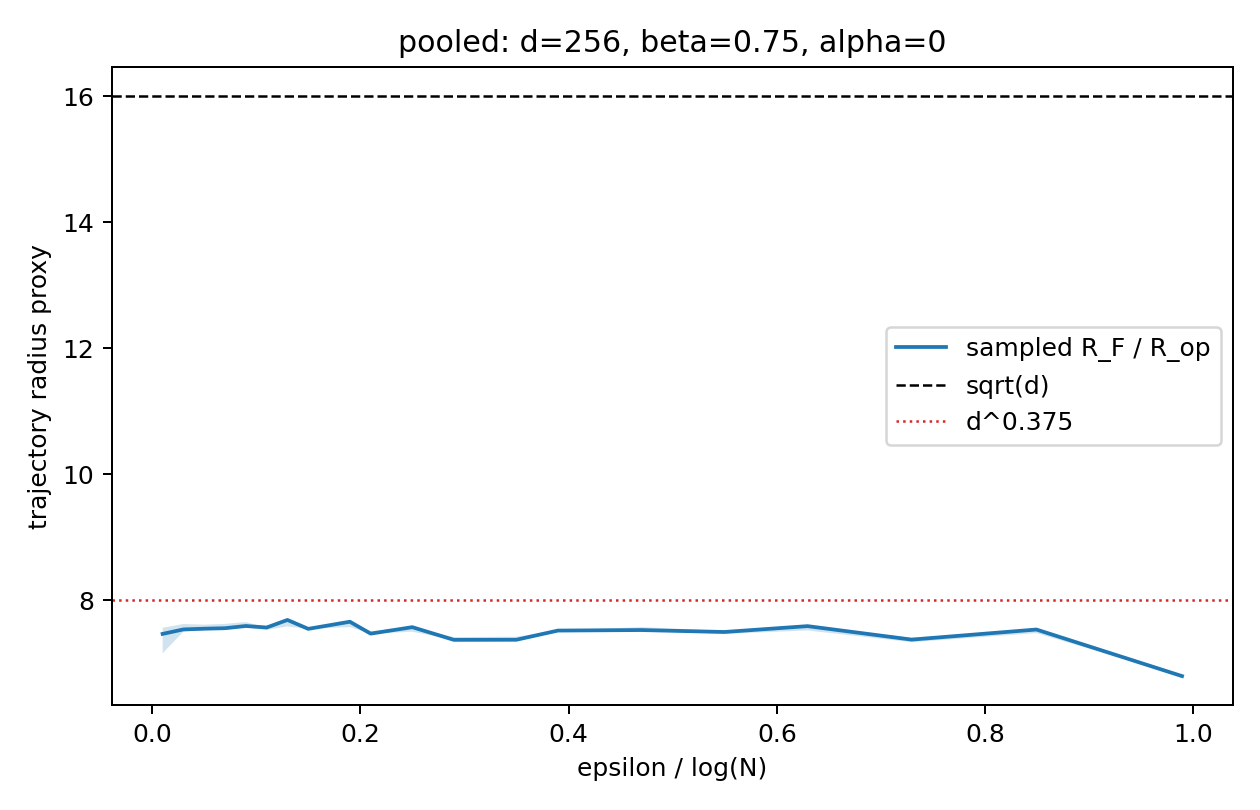
\includegraphics[width=\linewidth]{figures/trajectory_radius_proxy_pooled/radius_proxy_pooled_d256_b0.75_a0.png}
\caption{$\alpha=0$}
\end{subfigure}%
\hfill
\begin{subfigure}{0.22\textwidth}
\centering
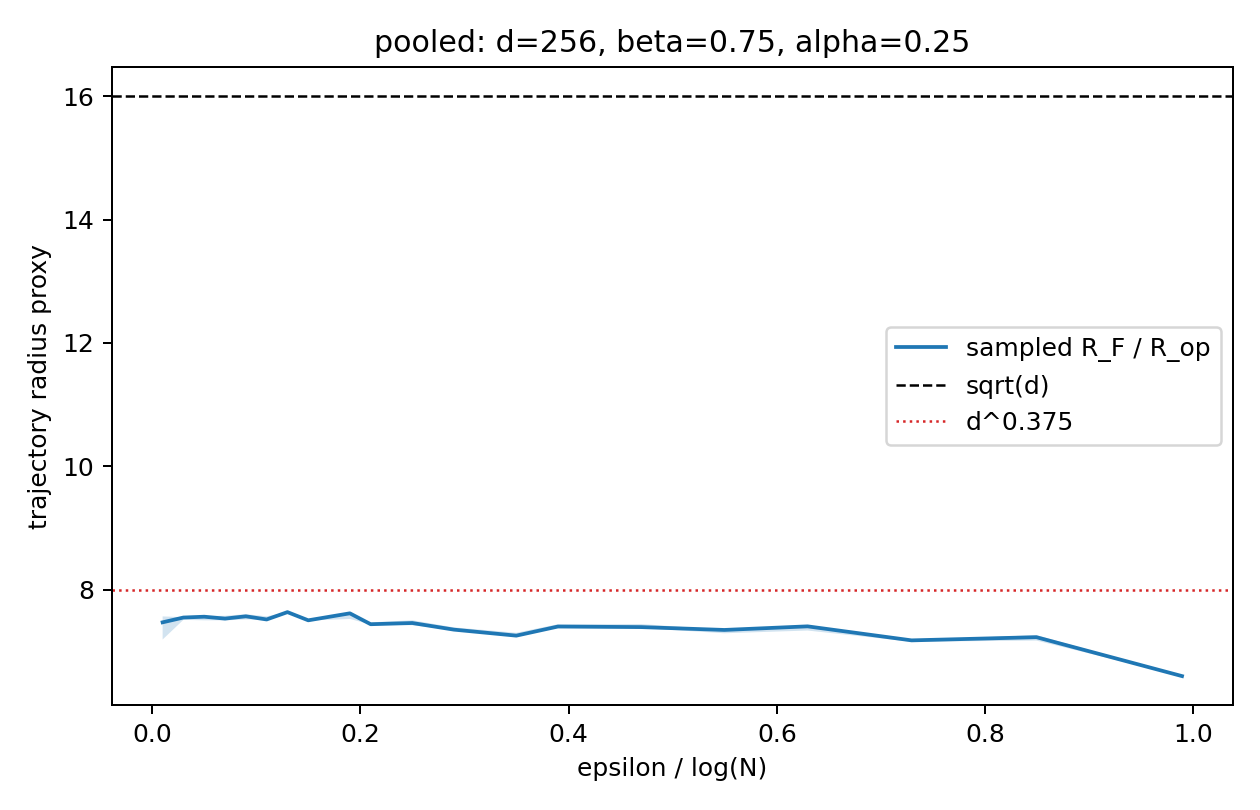
\includegraphics[width=\linewidth]{figures/trajectory_radius_proxy_pooled/radius_proxy_pooled_d256_b0.75_a0.25.png}
\caption{$\alpha=0.25$}
\end{subfigure}%
\hfill
\begin{subfigure}{0.22\textwidth}
\centering
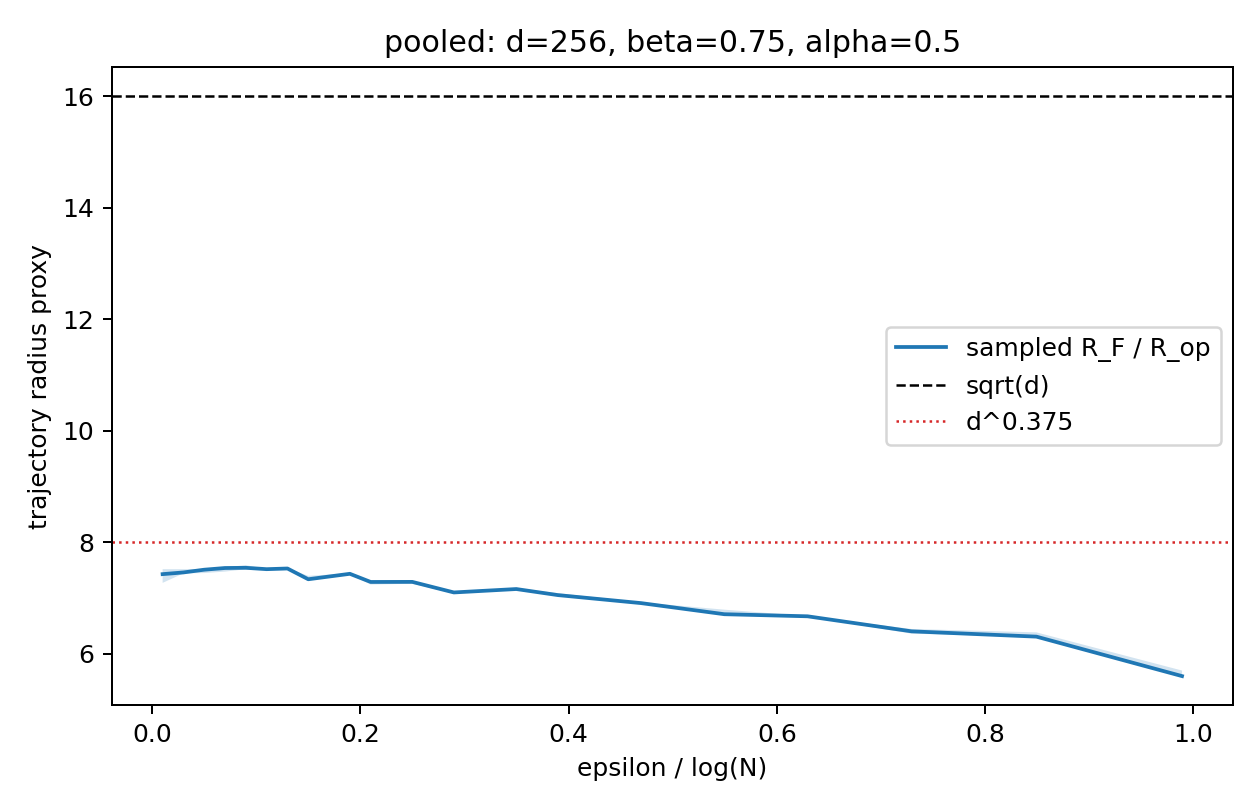
\includegraphics[width=\linewidth]{figures/trajectory_radius_proxy_pooled/radius_proxy_pooled_d256_b0.75_a0.5.png}
\caption{$\alpha=0.5$}
\end{subfigure}%
\hfill
\begin{subfigure}{0.22\textwidth}
\centering
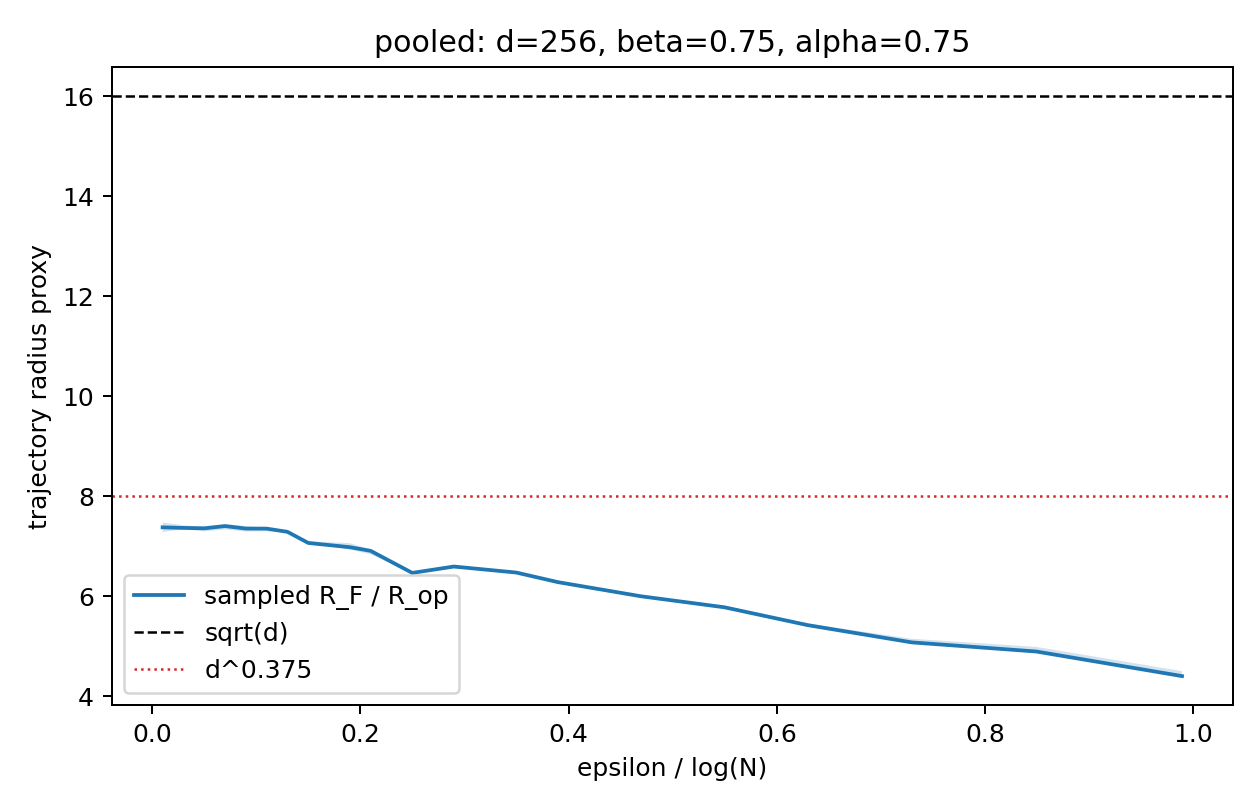
\includegraphics[width=\linewidth]{figures/trajectory_radius_proxy_pooled/radius_proxy_pooled_d256_b0.75_a0.75.png}
\caption{$\alpha=0.75$}
\end{subfigure}%
\par\smallskip
\begin{subfigure}{0.22\textwidth}
\centering
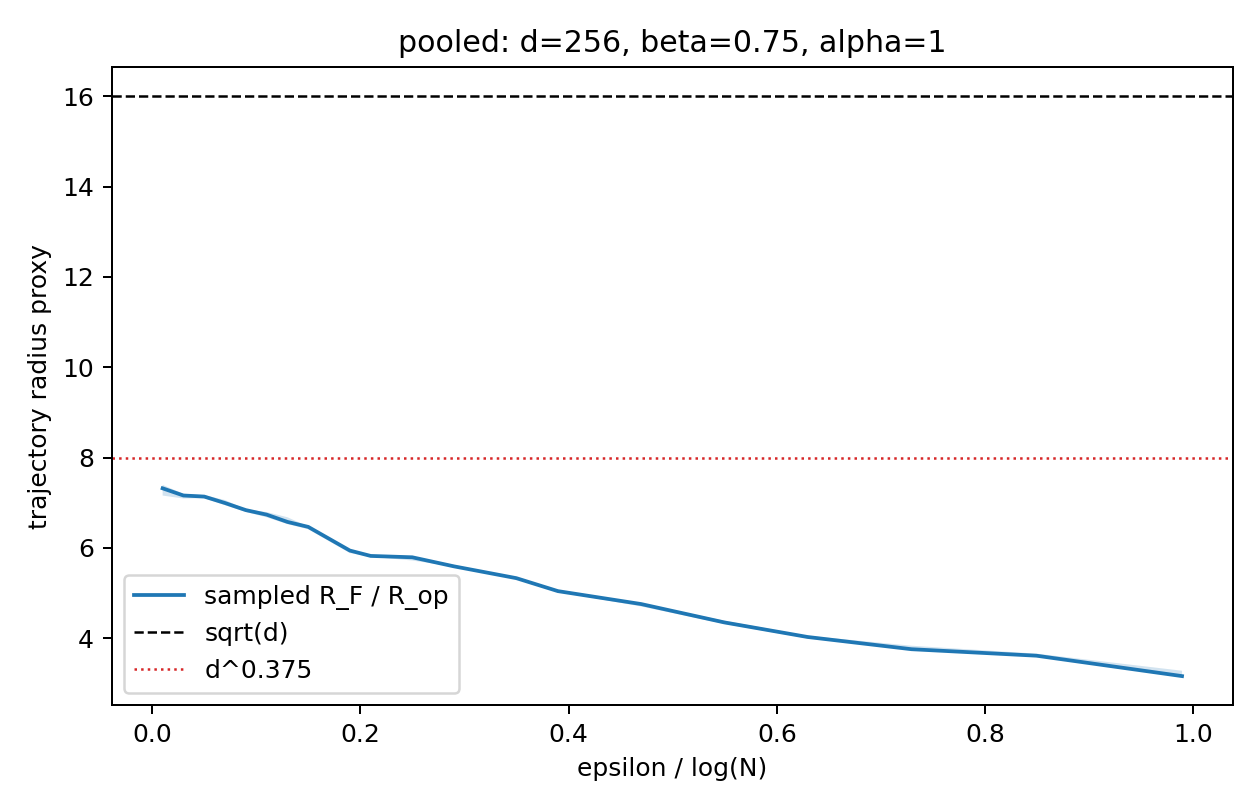
\includegraphics[width=\linewidth]{figures/trajectory_radius_proxy_pooled/radius_proxy_pooled_d256_b0.75_a1.png}
\caption{$\alpha=1$}
\end{subfigure}%
\hfill
\begin{subfigure}{0.22\textwidth}
\centering
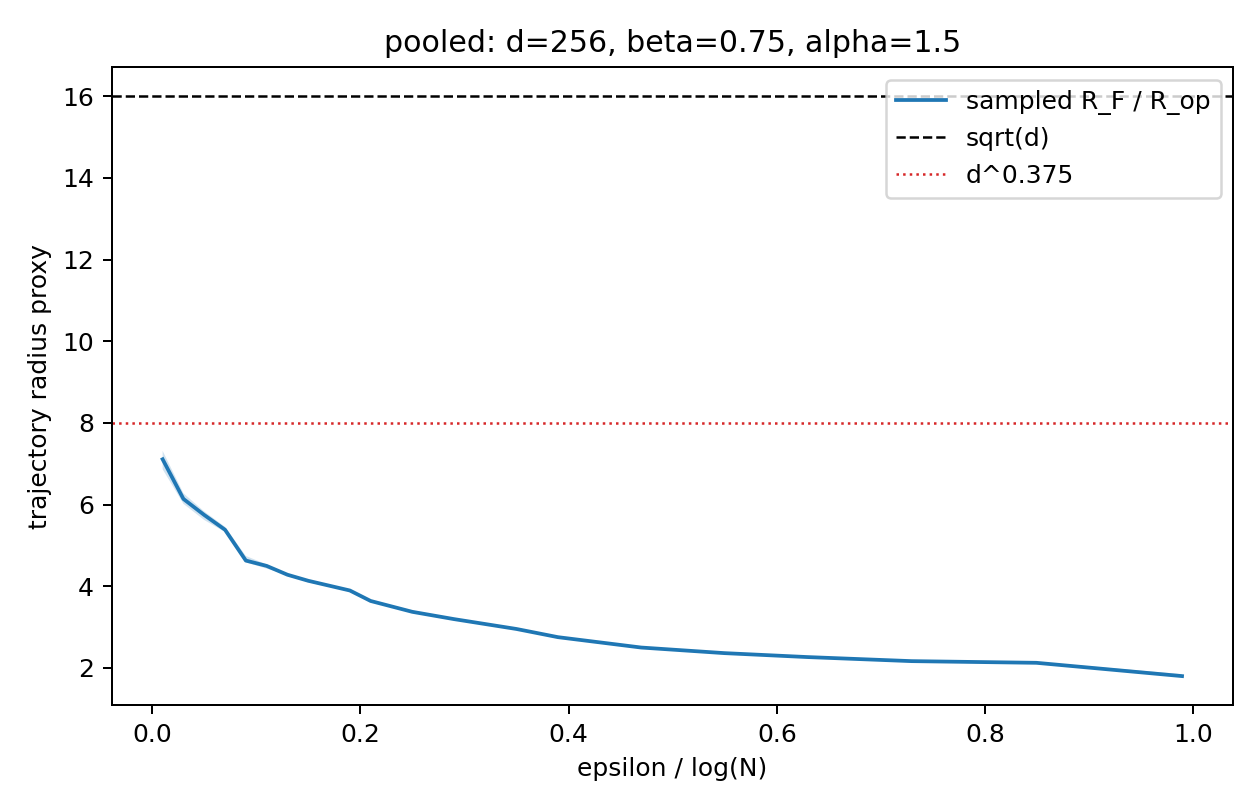
\includegraphics[width=\linewidth]{figures/trajectory_radius_proxy_pooled/radius_proxy_pooled_d256_b0.75_a1.5.png}
\caption{$\alpha=1.5$}
\end{subfigure}%
\hfill
\begin{subfigure}{0.22\textwidth}
\centering
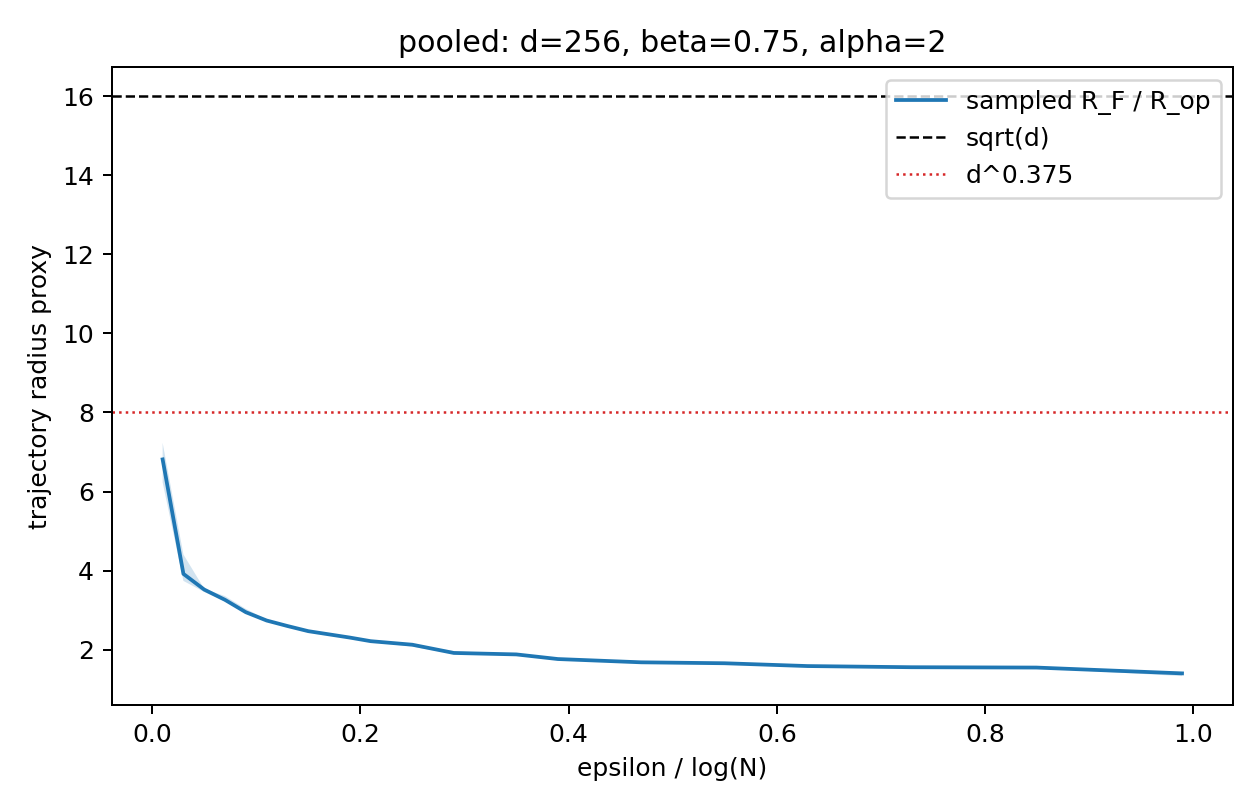
\includegraphics[width=\linewidth]{figures/trajectory_radius_proxy_pooled/radius_proxy_pooled_d256_b0.75_a2.png}
\caption{$\alpha=2$}
\end{subfigure}%
\caption{Pooled Trajectory Radius Proxy curves, $\beta=0.75$, $d=256$, $N=64$. Each panel is one value of $\alpha$. The solid line is the seed median and the shaded band is the interquartile range over three seeds.}
\label{fig:radius_proxy:pooled:b075}
\end{figure}

\begin{figure}[H]
\centering
\begin{subfigure}{0.22\textwidth}
\centering
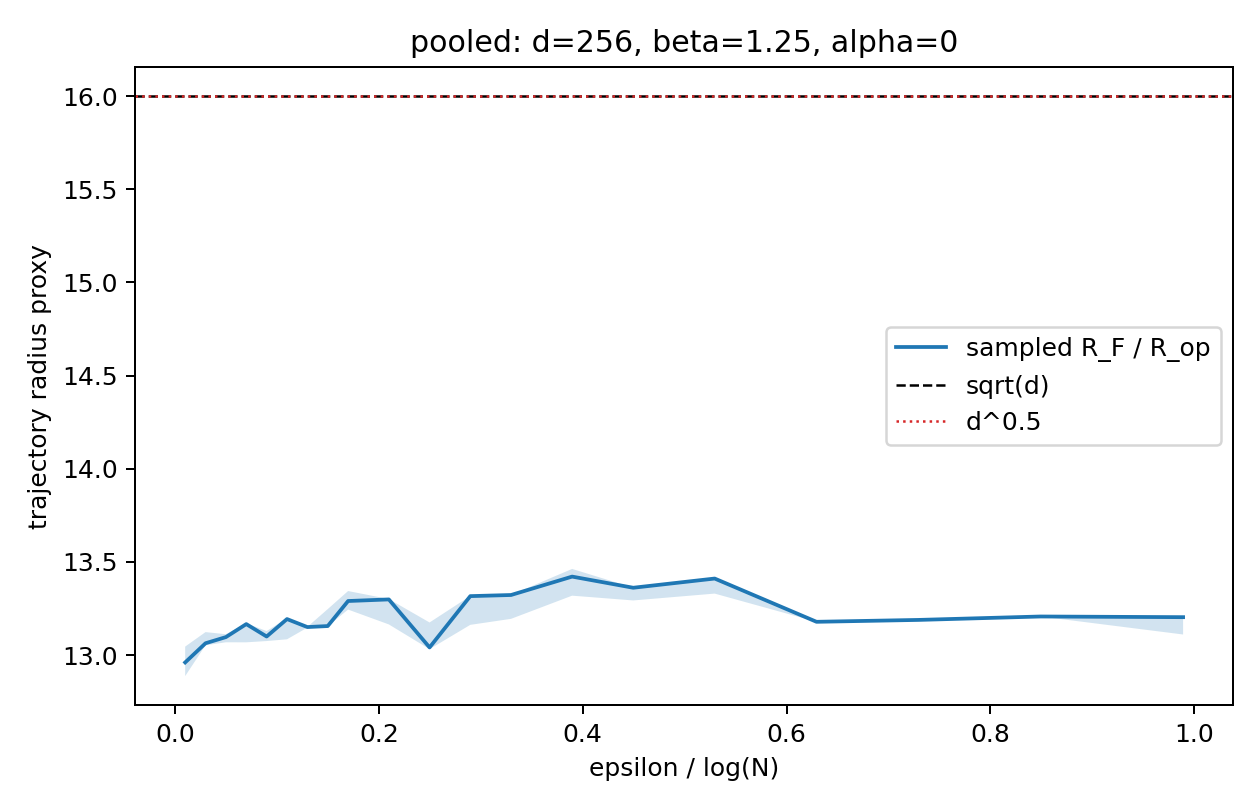
\includegraphics[width=\linewidth]{figures/trajectory_radius_proxy_pooled/radius_proxy_pooled_d256_b1.25_a0.png}
\caption{$\alpha=0$}
\end{subfigure}%
\hfill
\begin{subfigure}{0.22\textwidth}
\centering
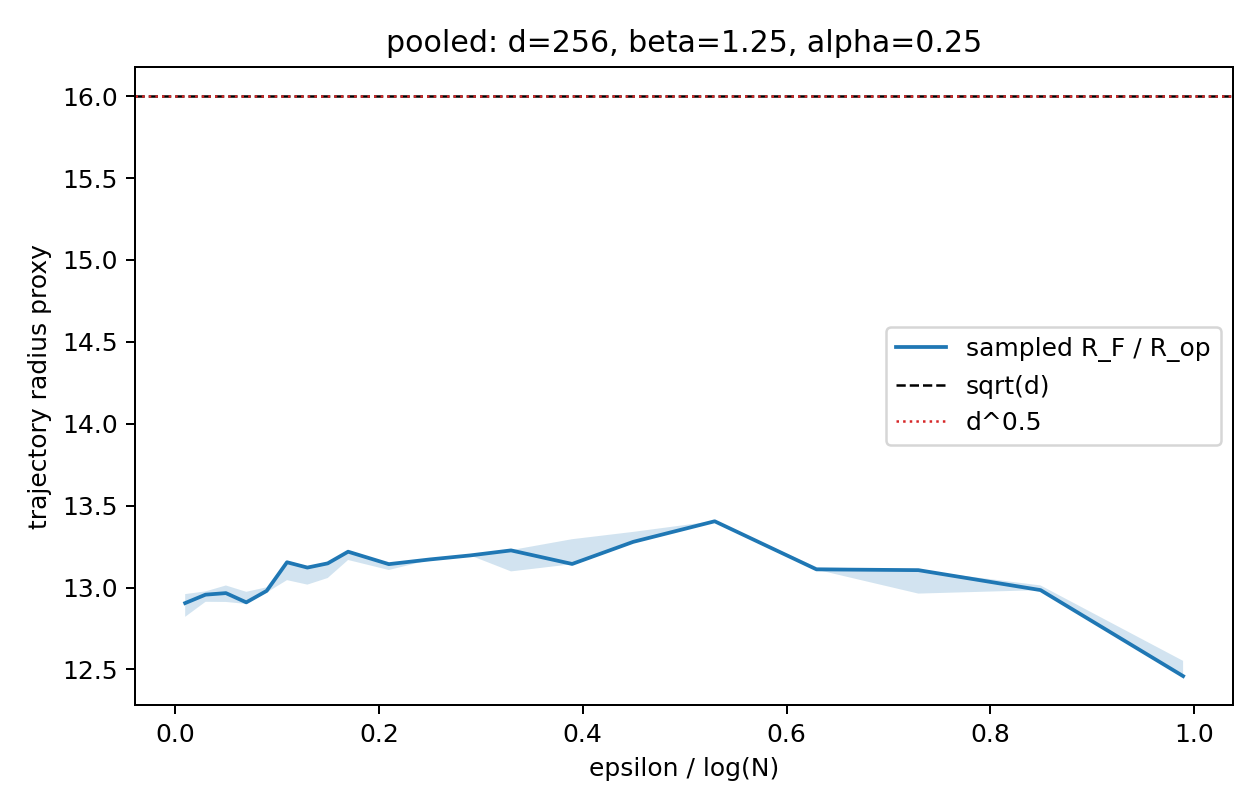
\includegraphics[width=\linewidth]{figures/trajectory_radius_proxy_pooled/radius_proxy_pooled_d256_b1.25_a0.25.png}
\caption{$\alpha=0.25$}
\end{subfigure}%
\hfill
\begin{subfigure}{0.22\textwidth}
\centering
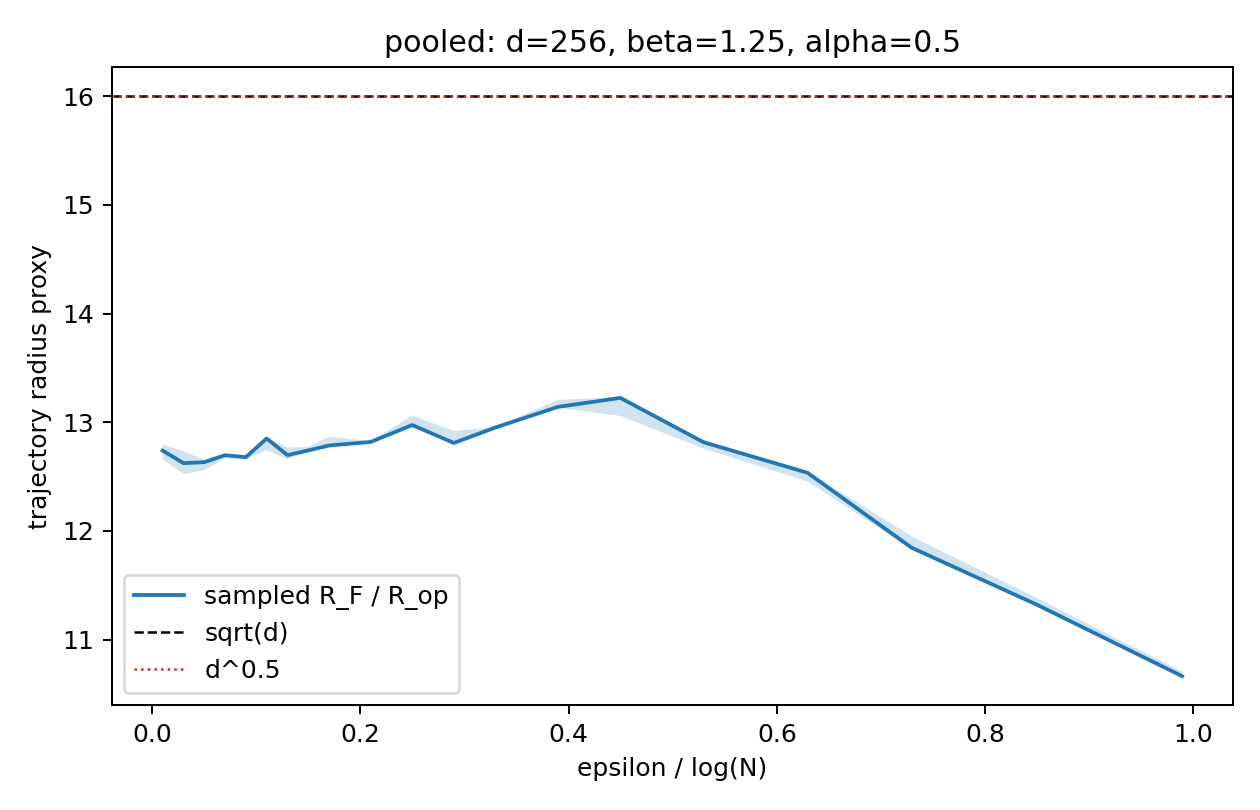
\includegraphics[width=\linewidth]{figures/trajectory_radius_proxy_pooled/radius_proxy_pooled_d256_b1.25_a0.5.png}
\caption{$\alpha=0.5$}
\end{subfigure}%
\hfill
\begin{subfigure}{0.22\textwidth}
\centering
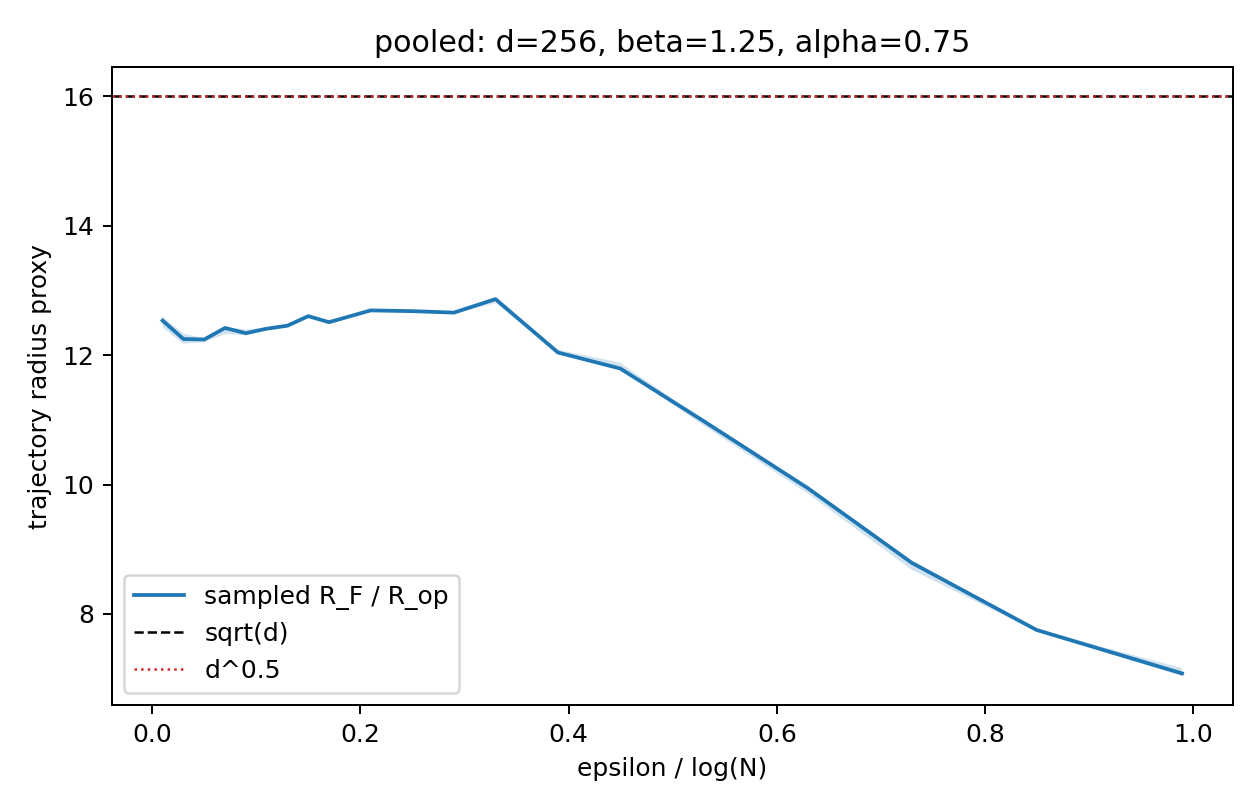
\includegraphics[width=\linewidth]{figures/trajectory_radius_proxy_pooled/radius_proxy_pooled_d256_b1.25_a0.75.png}
\caption{$\alpha=0.75$}
\end{subfigure}%
\par\smallskip
\begin{subfigure}{0.22\textwidth}
\centering
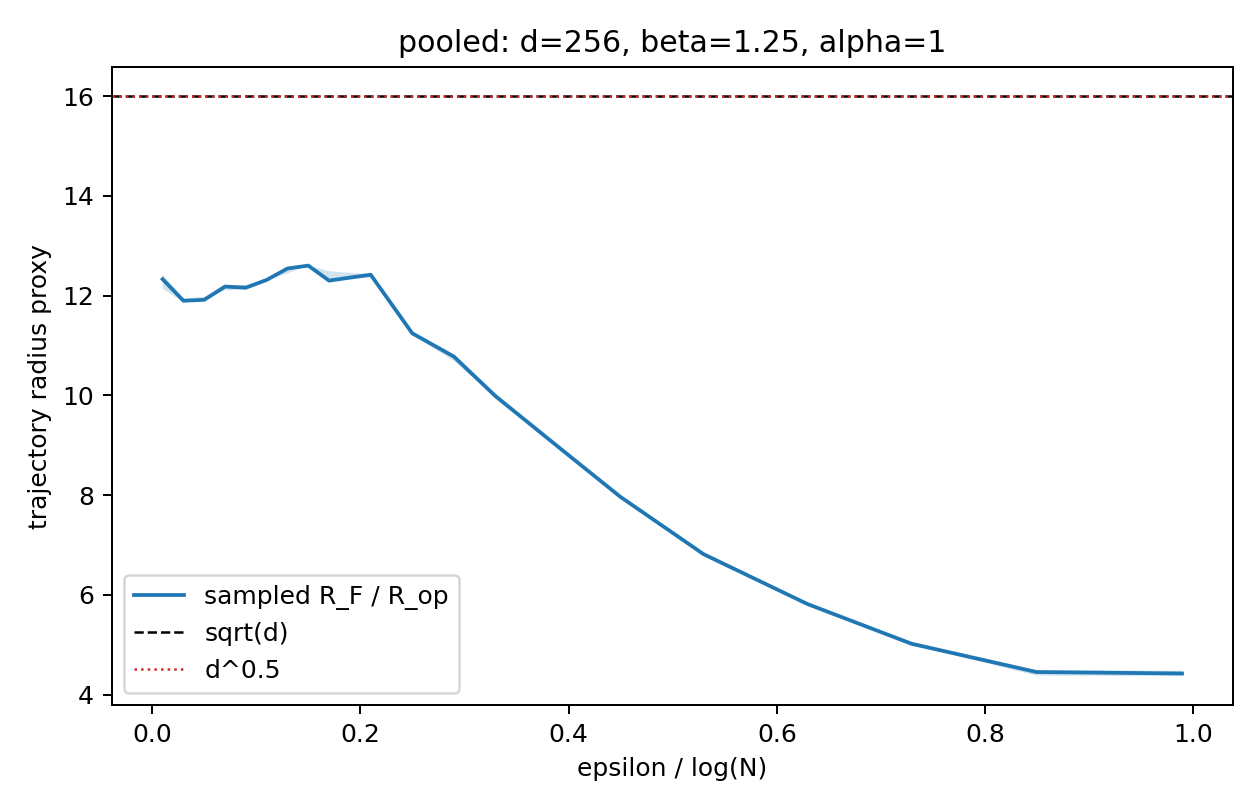
\includegraphics[width=\linewidth]{figures/trajectory_radius_proxy_pooled/radius_proxy_pooled_d256_b1.25_a1.png}
\caption{$\alpha=1$}
\end{subfigure}%
\hfill
\begin{subfigure}{0.22\textwidth}
\centering
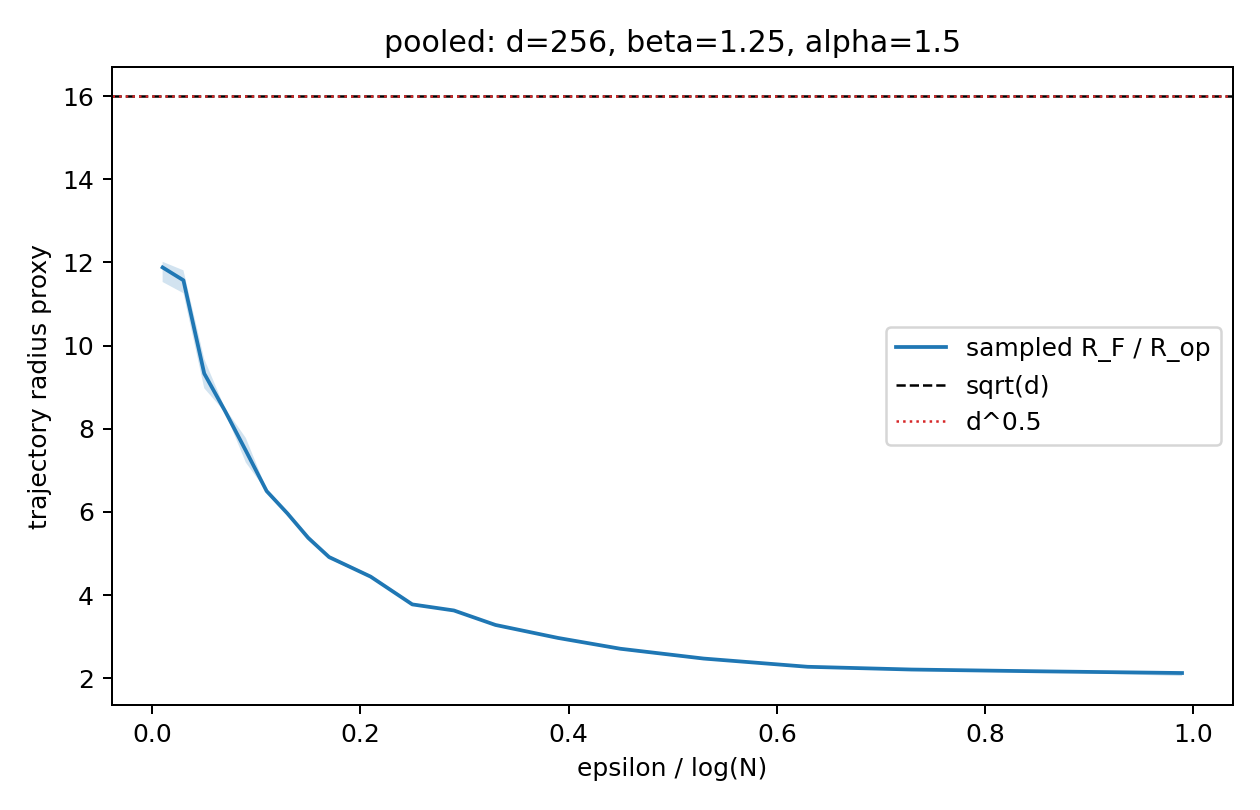
\includegraphics[width=\linewidth]{figures/trajectory_radius_proxy_pooled/radius_proxy_pooled_d256_b1.25_a1.5.png}
\caption{$\alpha=1.5$}
\end{subfigure}%
\hfill
\begin{subfigure}{0.22\textwidth}
\centering
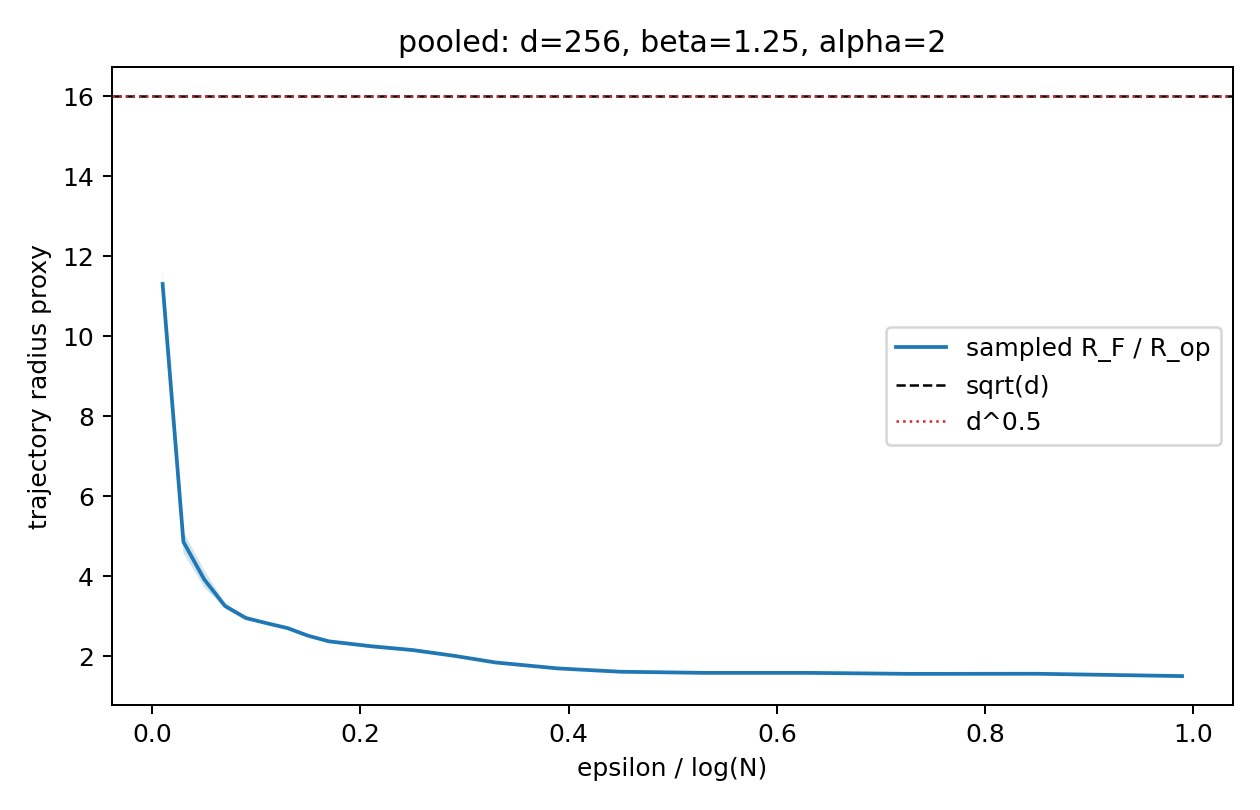
\includegraphics[width=\linewidth]{figures/trajectory_radius_proxy_pooled/radius_proxy_pooled_d256_b1.25_a2.png}
\caption{$\alpha=2$}
\end{subfigure}%
\caption{Pooled Trajectory Radius Proxy curves, $\beta=1.25$, $d=256$, $N=1024$. Each panel is one value of $\alpha$. The solid line is the seed median and the shaded band is the interquartile range over three seeds.}
\label{fig:radius_proxy:pooled:b125}
\end{figure}

\begin{figure}[H]
\centering
\begin{subfigure}{0.22\textwidth}
\centering
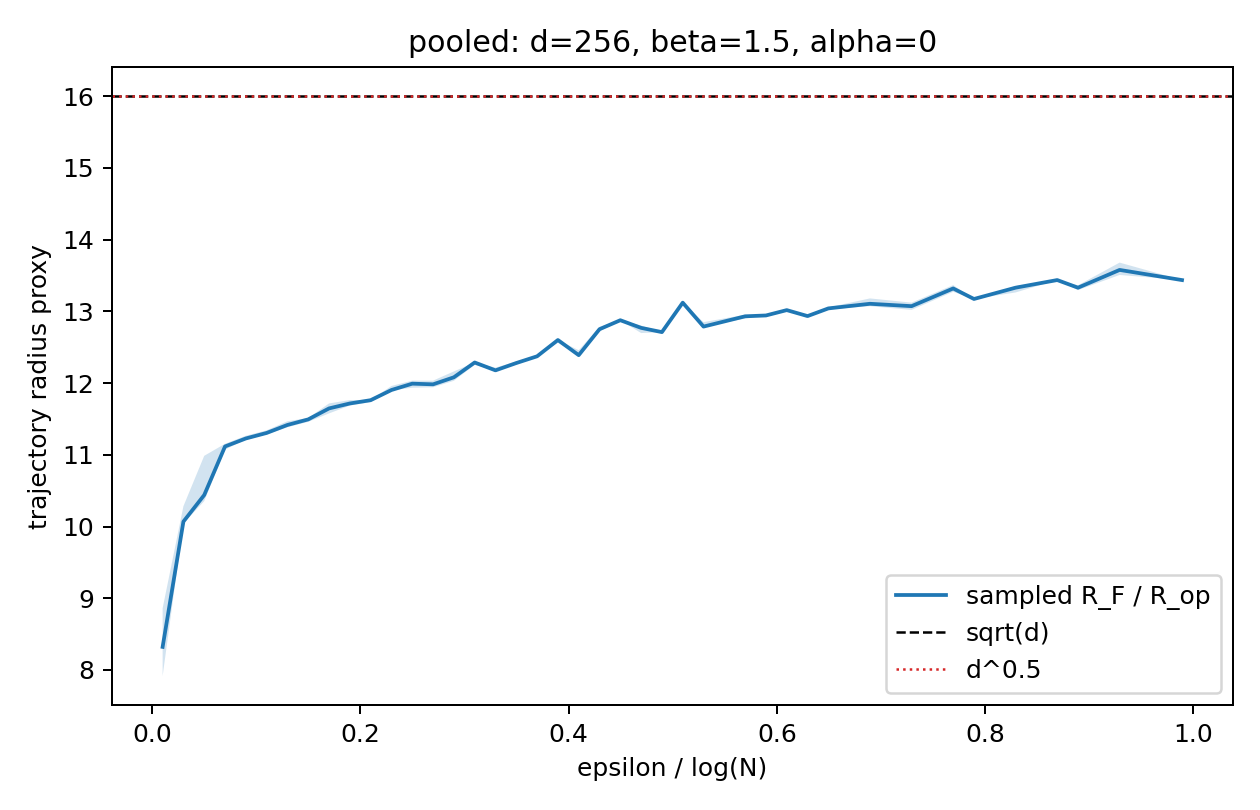
\includegraphics[width=\linewidth]{figures/trajectory_radius_proxy_pooled/radius_proxy_pooled_d256_b1.5_a0.png}
\caption{$\alpha=0$}
\end{subfigure}%
\hfill
\begin{subfigure}{0.22\textwidth}
\centering
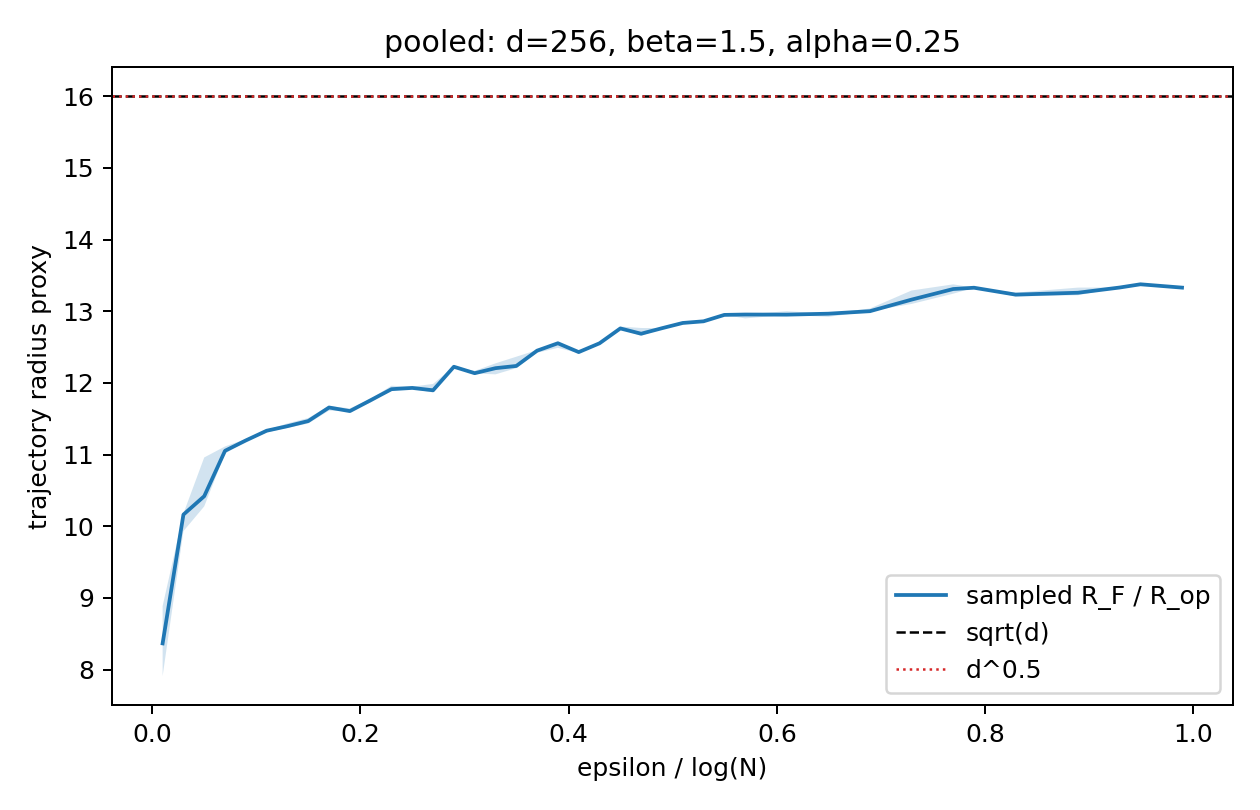
\includegraphics[width=\linewidth]{figures/trajectory_radius_proxy_pooled/radius_proxy_pooled_d256_b1.5_a0.25.png}
\caption{$\alpha=0.25$}
\end{subfigure}%
\hfill
\begin{subfigure}{0.22\textwidth}
\centering
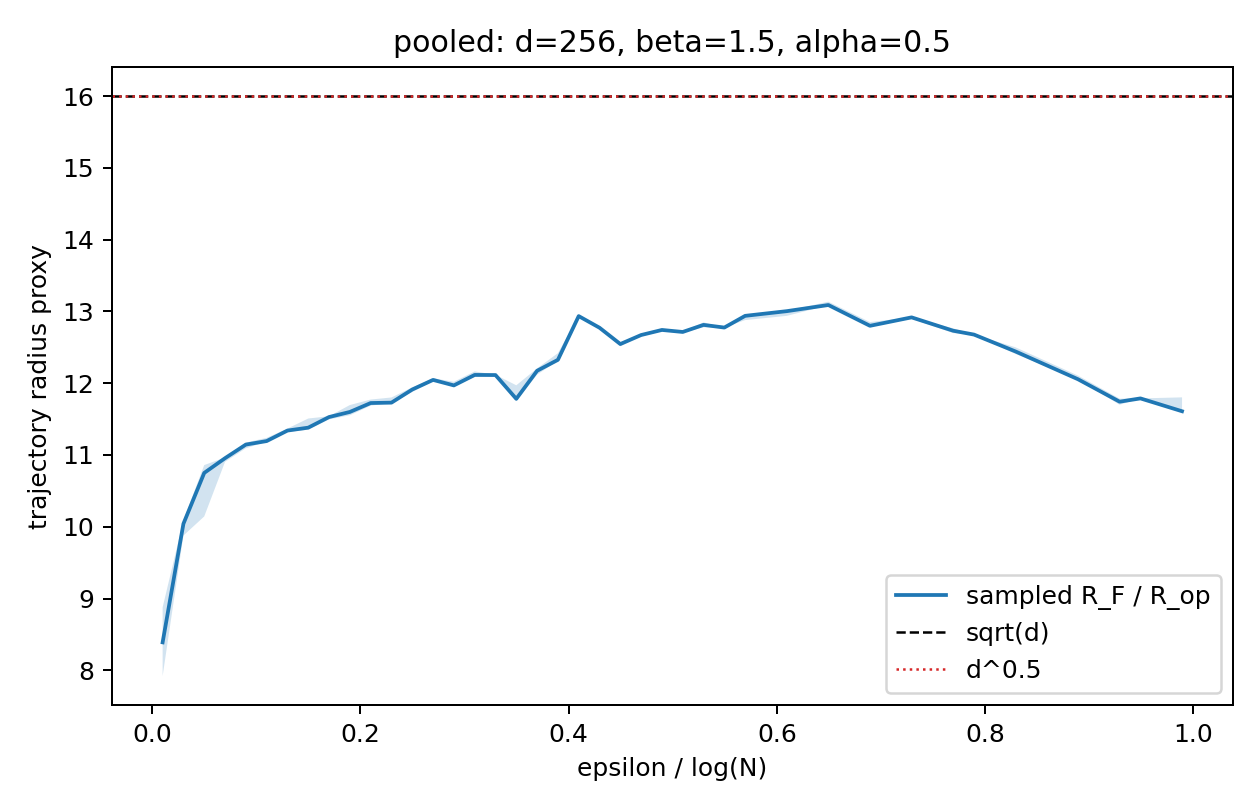
\includegraphics[width=\linewidth]{figures/trajectory_radius_proxy_pooled/radius_proxy_pooled_d256_b1.5_a0.5.png}
\caption{$\alpha=0.5$}
\end{subfigure}%
\hfill
\begin{subfigure}{0.22\textwidth}
\centering
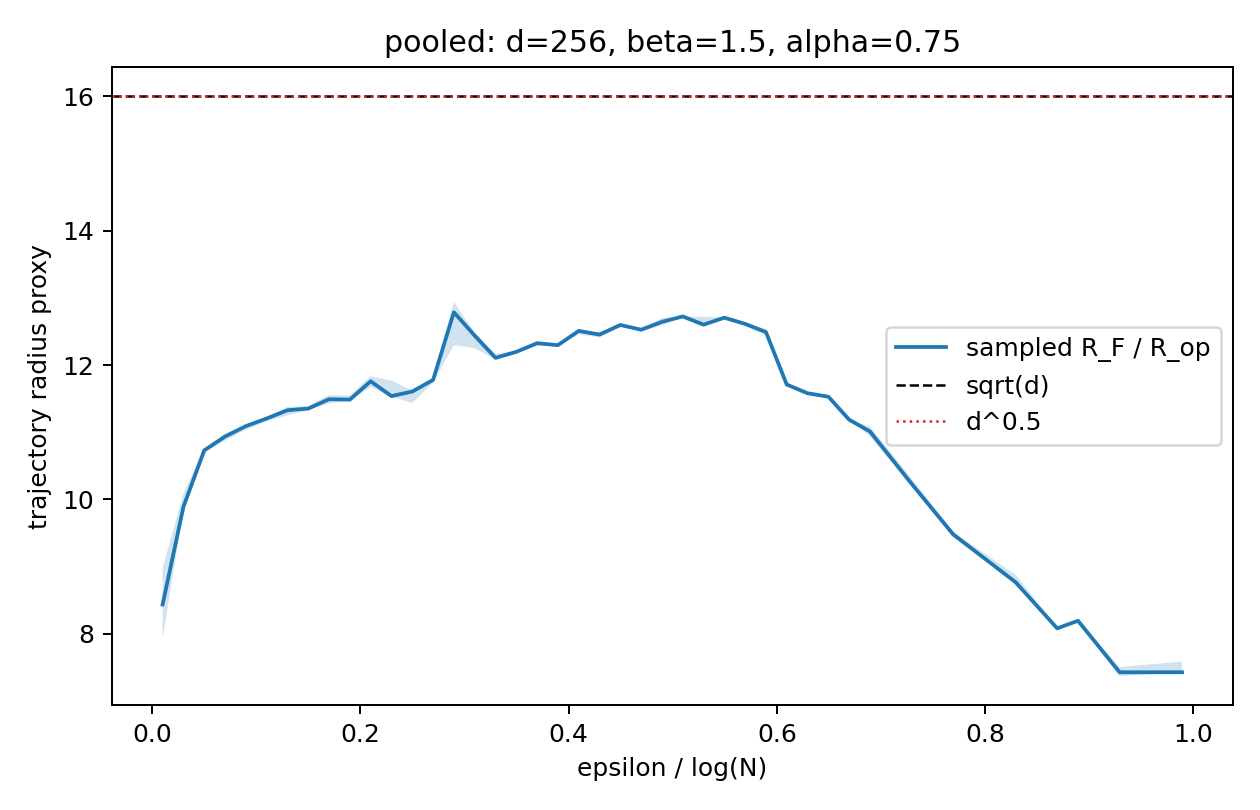
\includegraphics[width=\linewidth]{figures/trajectory_radius_proxy_pooled/radius_proxy_pooled_d256_b1.5_a0.75.png}
\caption{$\alpha=0.75$}
\end{subfigure}%
\par\smallskip
\begin{subfigure}{0.22\textwidth}
\centering
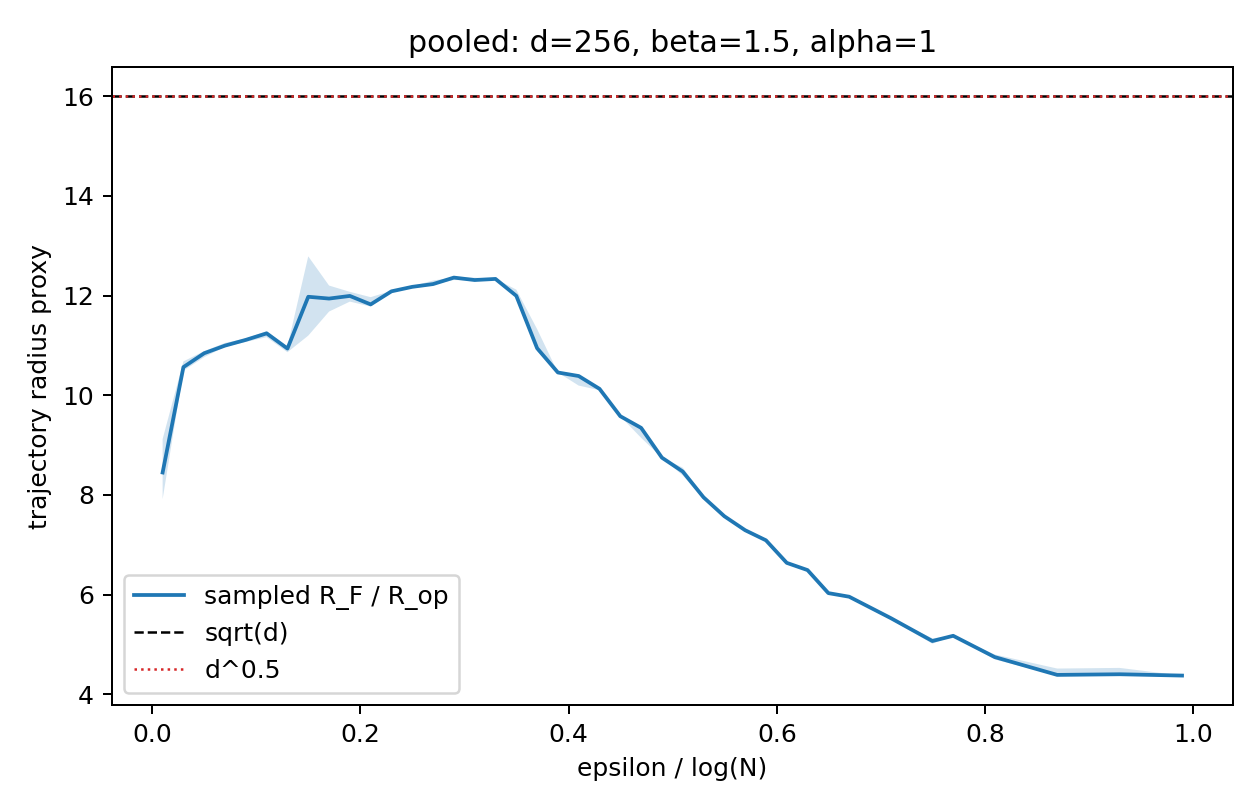
\includegraphics[width=\linewidth]{figures/trajectory_radius_proxy_pooled/radius_proxy_pooled_d256_b1.5_a1.png}
\caption{$\alpha=1$}
\end{subfigure}%
\hfill
\begin{subfigure}{0.22\textwidth}
\centering
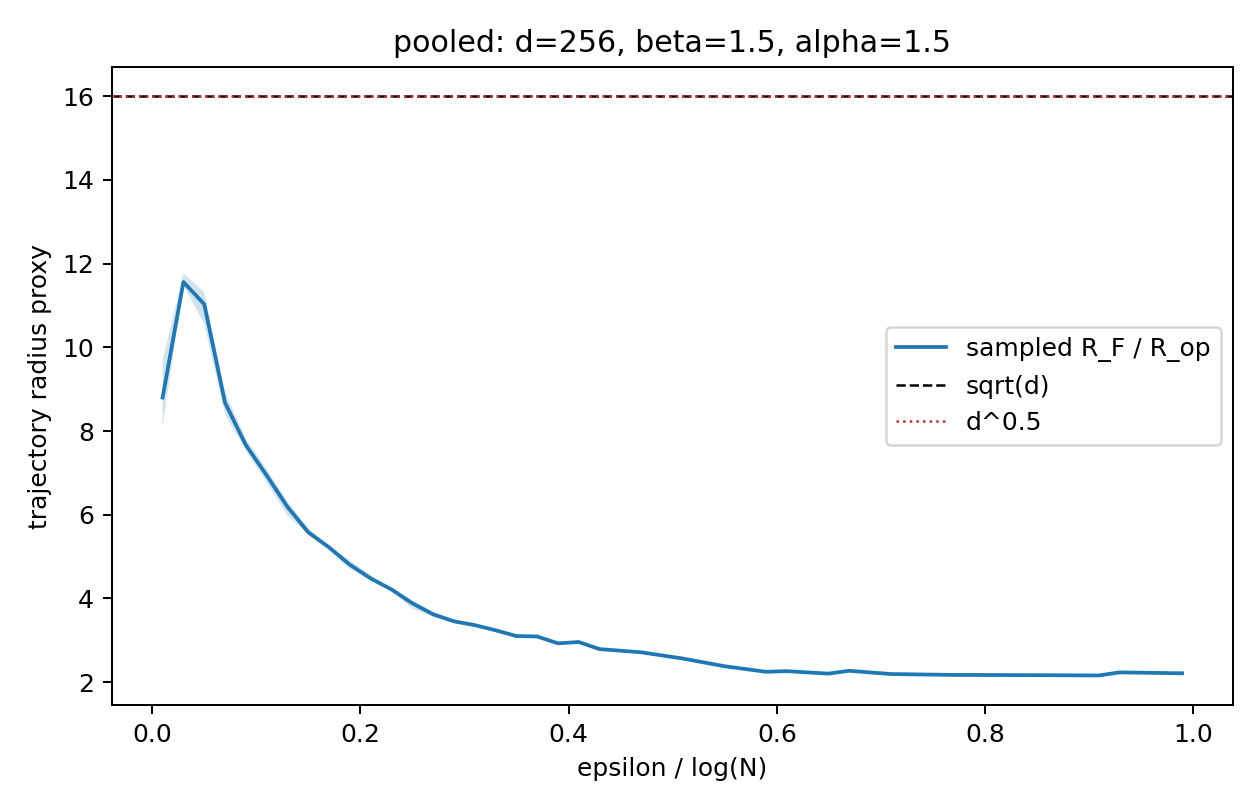
\includegraphics[width=\linewidth]{figures/trajectory_radius_proxy_pooled/radius_proxy_pooled_d256_b1.5_a1.5.png}
\caption{$\alpha=1.5$}
\end{subfigure}%
\hfill
\begin{subfigure}{0.22\textwidth}
\centering
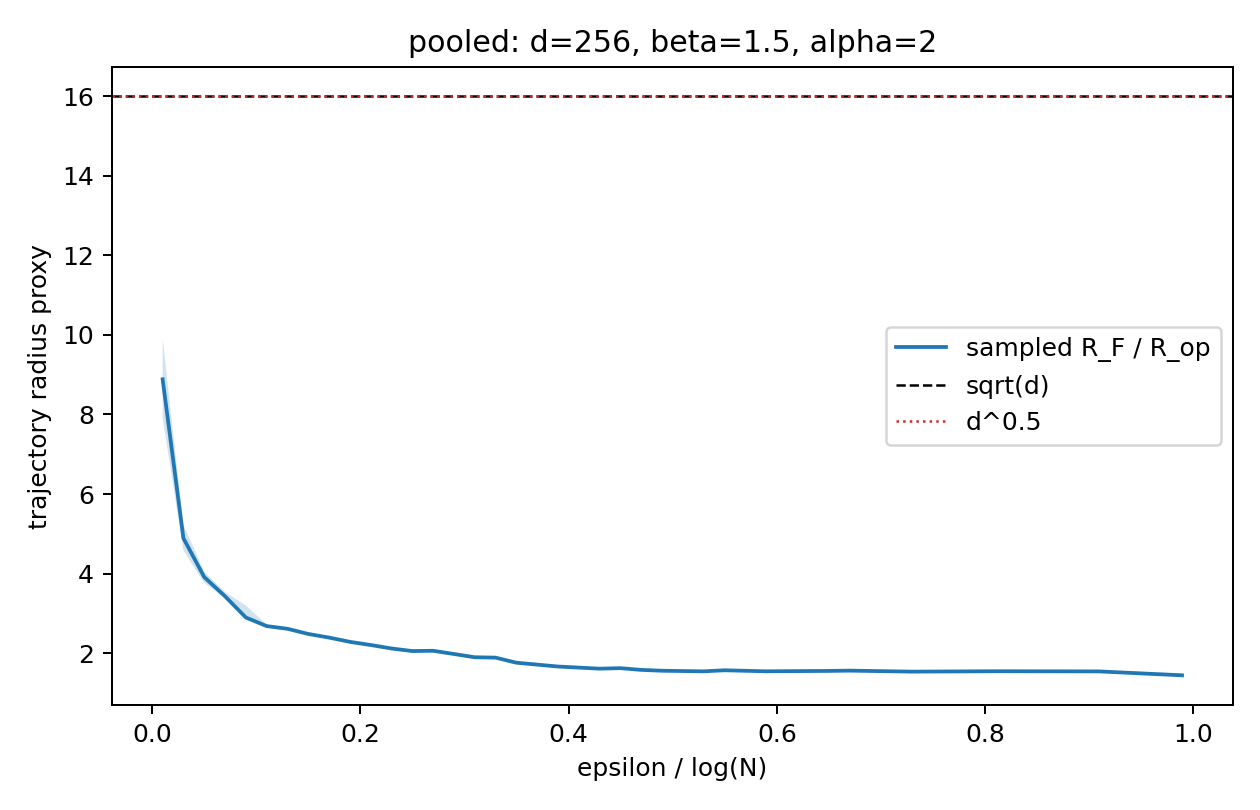
\includegraphics[width=\linewidth]{figures/trajectory_radius_proxy_pooled/radius_proxy_pooled_d256_b1.5_a2.png}
\caption{$\alpha=2$}
\end{subfigure}%
\caption{Pooled Trajectory Radius Proxy curves, $\beta=1.5$, $d=256$, $N=4096$. Each panel is one value of $\alpha$. The solid line is the seed median and the shaded band is the interquartile range over three seeds.}
\label{fig:radius_proxy:pooled:b15}
\end{figure}

\begin{figure}[H]
\centering
\begin{subfigure}{0.22\textwidth}
\centering
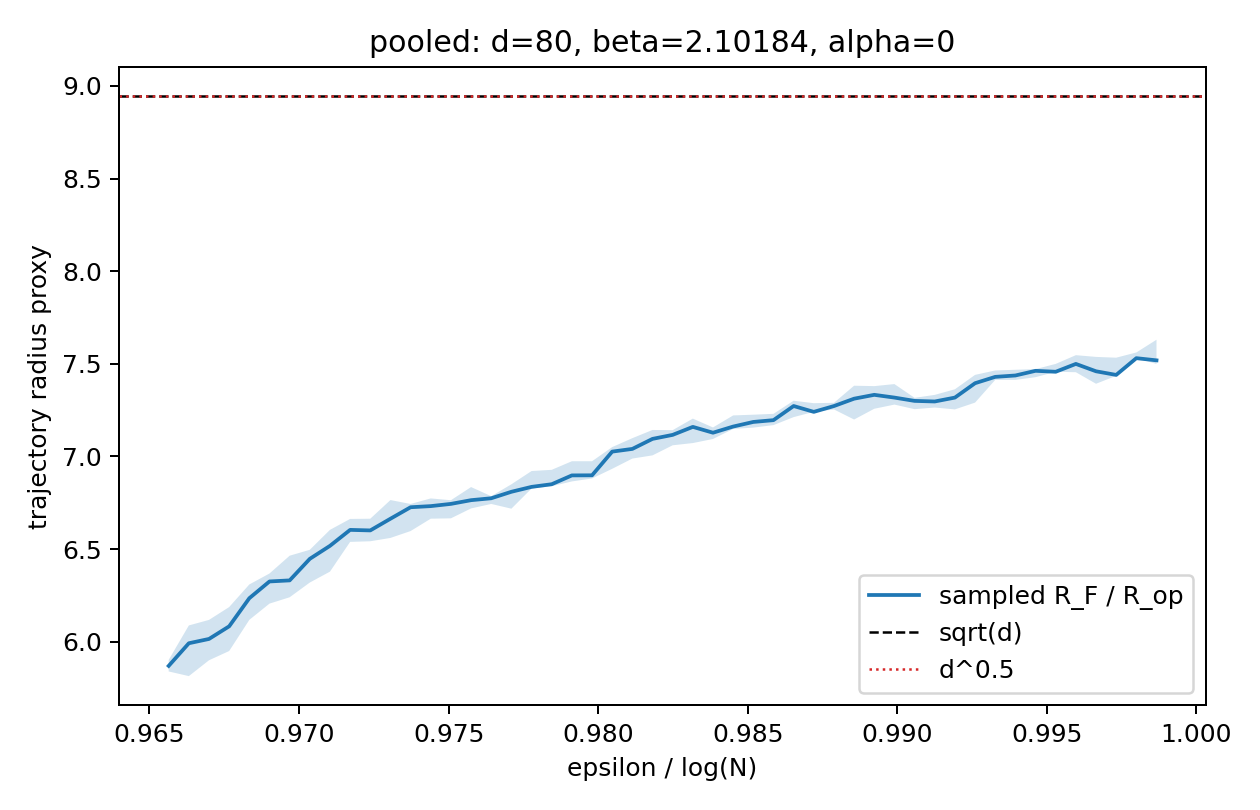
\includegraphics[width=\linewidth]{figures/trajectory_radius_proxy_pooled/radius_proxy_pooled_d80_b2.10184_a0.png}
\caption{$\alpha=0$}
\end{subfigure}%
\hfill
\begin{subfigure}{0.22\textwidth}
\centering
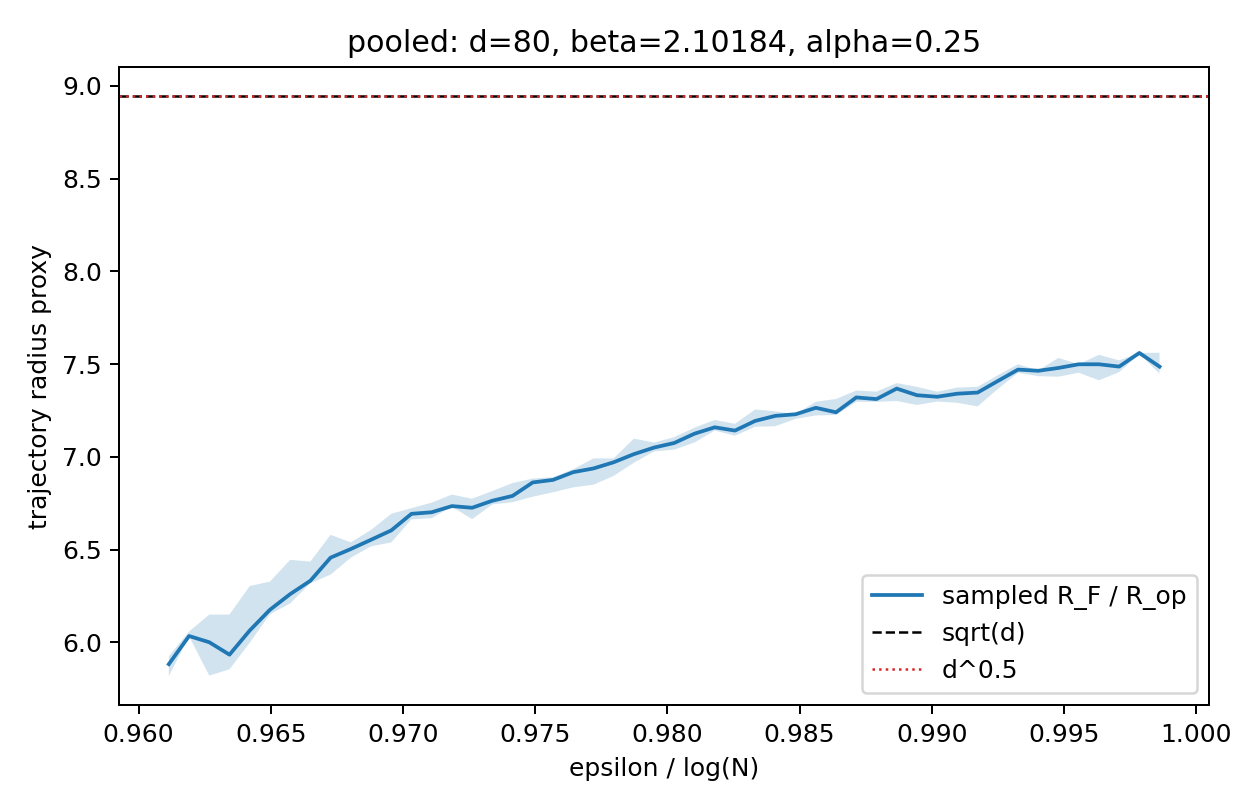
\includegraphics[width=\linewidth]{figures/trajectory_radius_proxy_pooled/radius_proxy_pooled_d80_b2.10184_a0.25.png}
\caption{$\alpha=0.25$}
\end{subfigure}%
\hfill
\begin{subfigure}{0.22\textwidth}
\centering
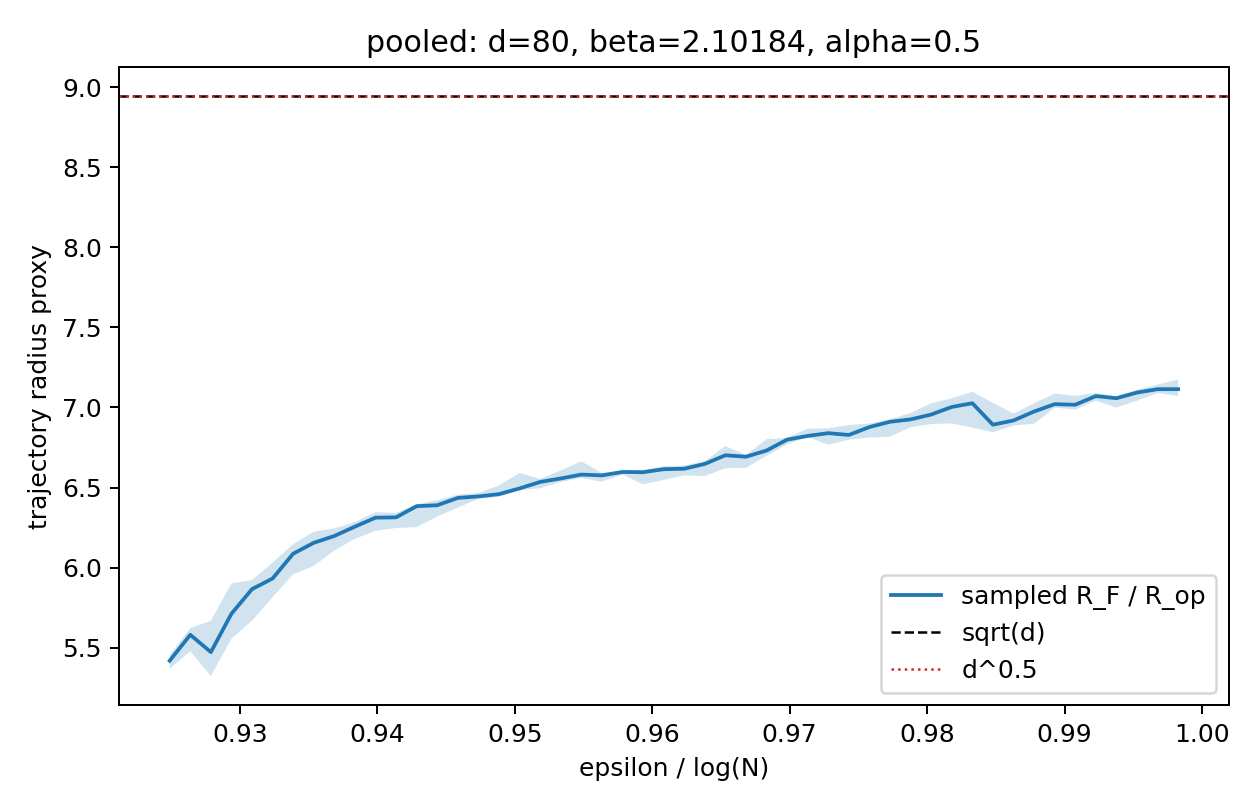
\includegraphics[width=\linewidth]{figures/trajectory_radius_proxy_pooled/radius_proxy_pooled_d80_b2.10184_a0.5.png}
\caption{$\alpha=0.5$}
\end{subfigure}%
\hfill
\begin{subfigure}{0.22\textwidth}
\centering
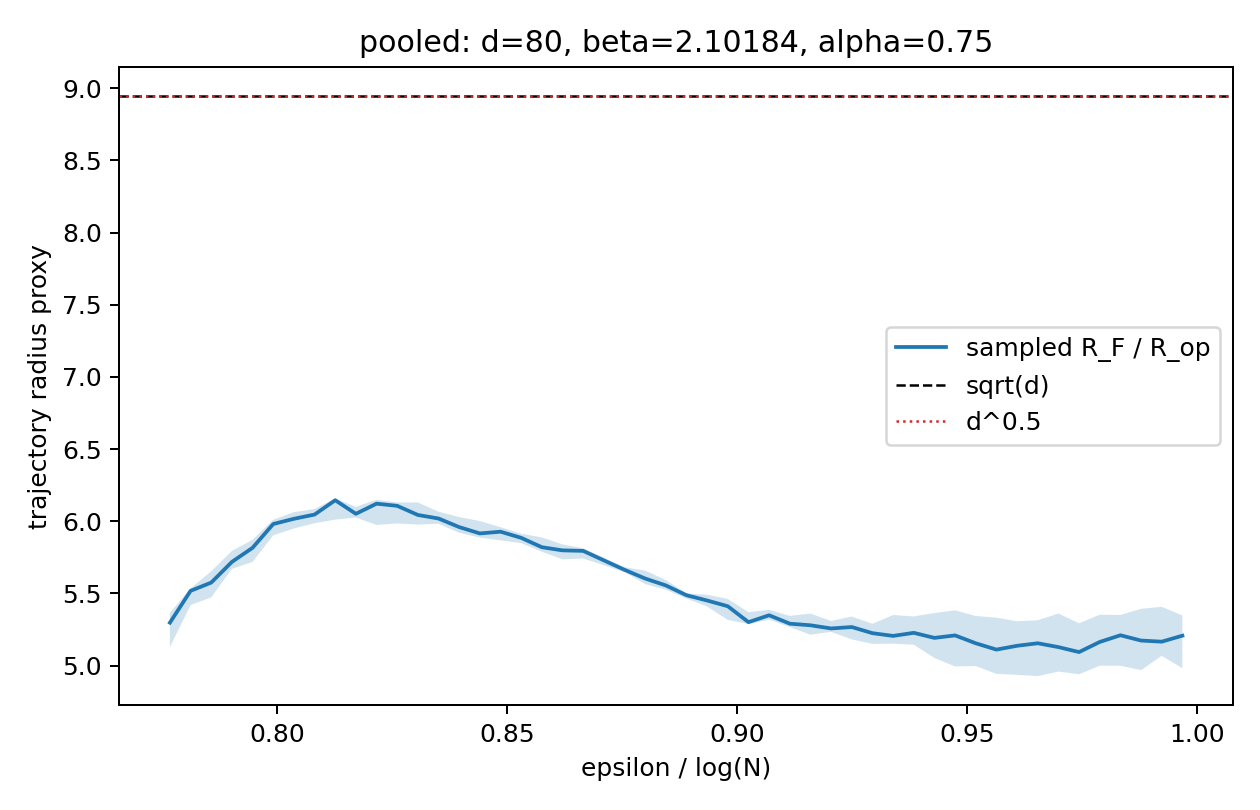
\includegraphics[width=\linewidth]{figures/trajectory_radius_proxy_pooled/radius_proxy_pooled_d80_b2.10184_a0.75.png}
\caption{$\alpha=0.75$}
\end{subfigure}%
\par\smallskip
\begin{subfigure}{0.22\textwidth}
\centering
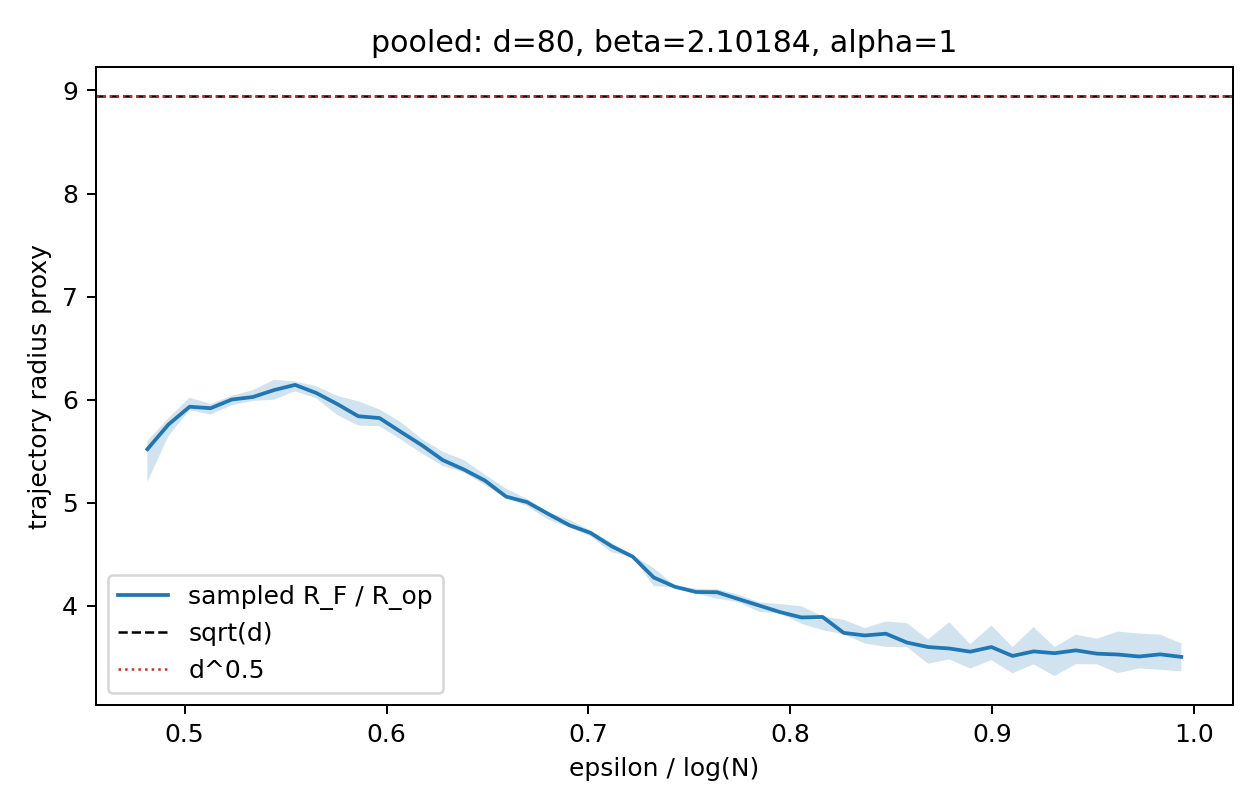
\includegraphics[width=\linewidth]{figures/trajectory_radius_proxy_pooled/radius_proxy_pooled_d80_b2.10184_a1.png}
\caption{$\alpha=1$}
\end{subfigure}%
\hfill
\begin{subfigure}{0.22\textwidth}
\centering
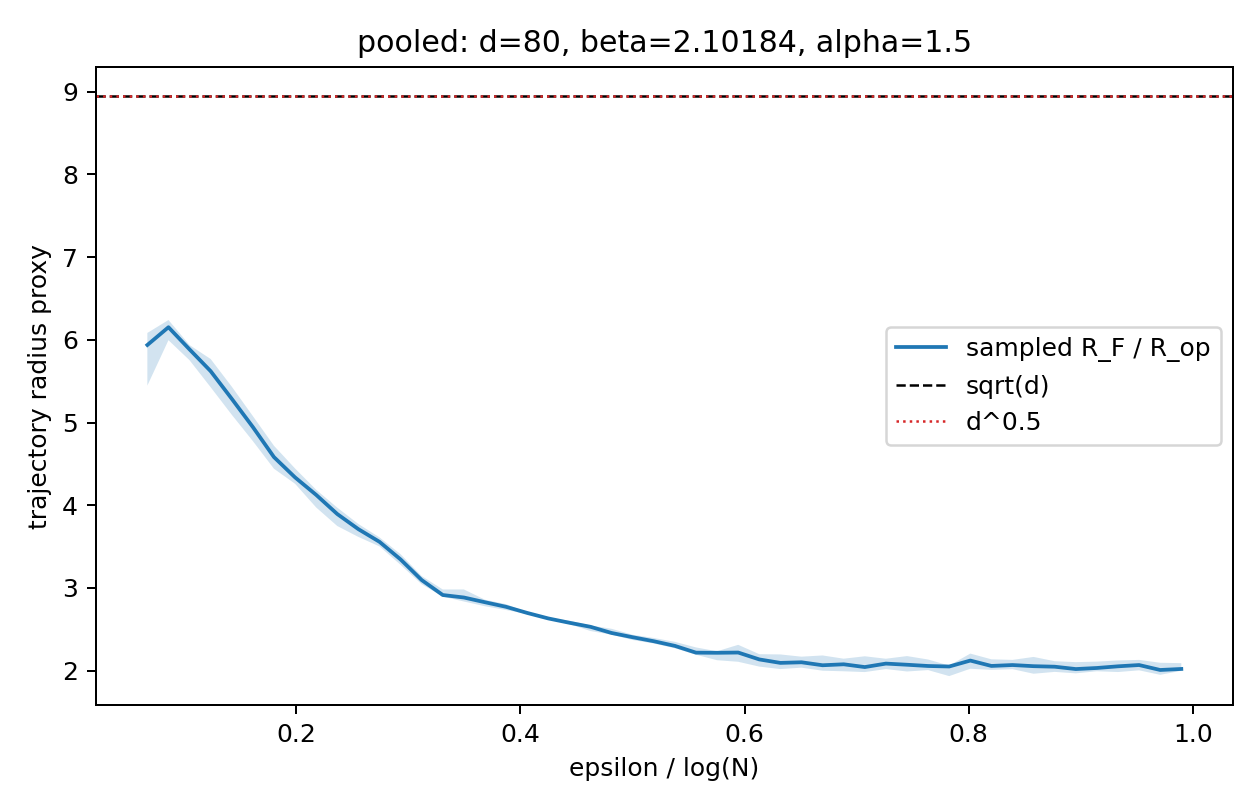
\includegraphics[width=\linewidth]{figures/trajectory_radius_proxy_pooled/radius_proxy_pooled_d80_b2.10184_a1.5.png}
\caption{$\alpha=1.5$}
\end{subfigure}%
\hfill
\begin{subfigure}{0.22\textwidth}
\centering
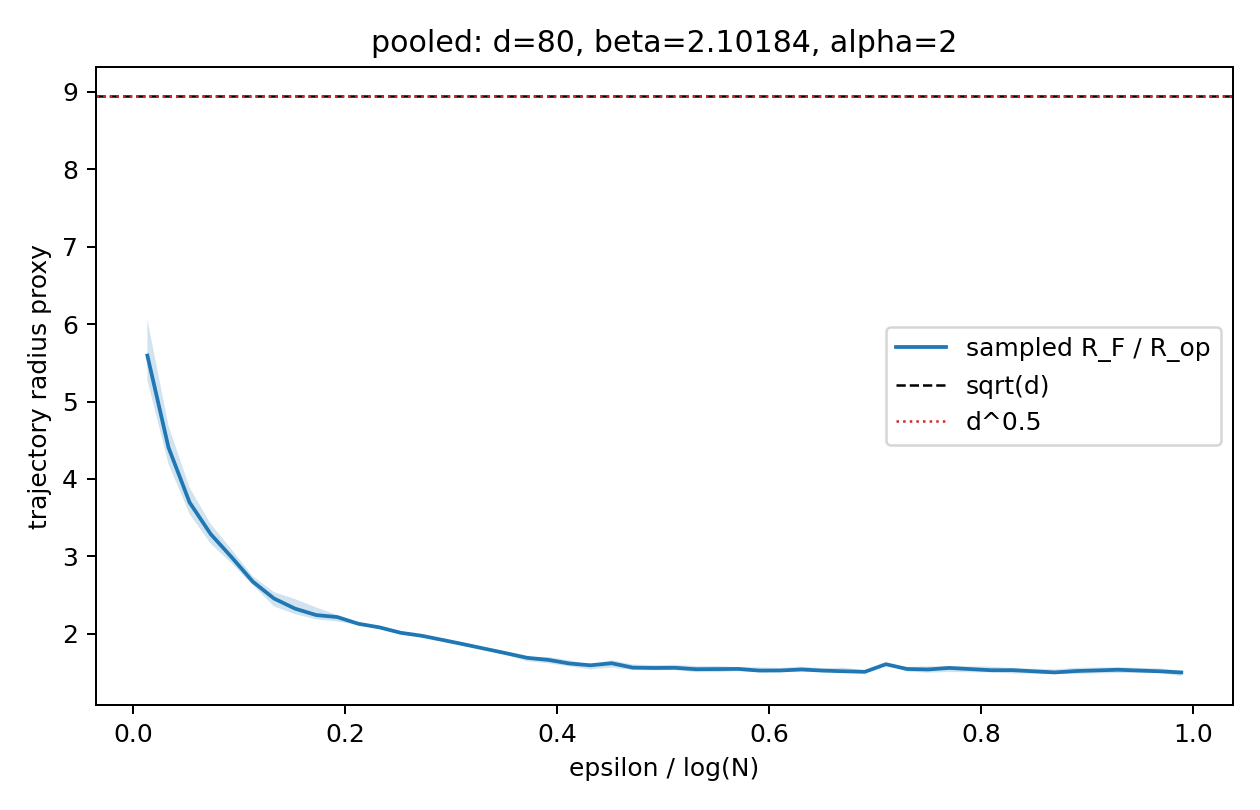
\includegraphics[width=\linewidth]{figures/trajectory_radius_proxy_pooled/radius_proxy_pooled_d80_b2.10184_a2.png}
\caption{$\alpha=2$}
\end{subfigure}%
\caption{Pooled Trajectory Radius Proxy curves, $\beta_{\rm eff}=2.101845$, $d=80$, $N=10000$. Each panel is one value of $\alpha$. The solid line is the seed median and the shaded band is the interquartile range over three seeds.}
\label{fig:radius_proxy:pooled:beff210}
\end{figure}




\section{Interpretation by experiment part}

\subsection{Realistic training}

The realistic-training experiment shows that Spectral-GD can provide a practical optimization advantage, but the advantage is not uniform. The strongest and cleanest block is $\beta=1.25$. In Figures~\ref{fig:realistic:loss:b125}--\ref{fig:realistic:T_ratio:b125}, the Spectral-GD curves improve with increasing $\alpha$, and the hitting-time ratio is above one for most target losses once $\alpha\geq 0.5$. This means the advantage is not merely a single lucky learning rate: it is visible in both the selected best-AUC traces and the epsilon-wise oracle hitting-time comparison.

The $\beta=1.5$ block is more nuanced. In Figures~\ref{fig:realistic:loss:b15}--\ref{fig:realistic:T_ratio:b15}, low $\alpha$ values, especially $\alpha=0$ and $\alpha=0.25$, favor NGD or show little Spectral-GD advantage. This is a genuine counterexample regime in the current experiment. As $\alpha$ increases, Spectral-GD recovers some advantage, and at $\alpha=2$ the median hitting-time ratio is above one. This supports the view that frequency heterogeneity is one of the drivers of the Spectral-GD benefit.

The fixed-large-$N$ proxy block has another distinct behavior. Low $\alpha$ gives essentially no speed advantage, but high $\alpha$ gives a moderate advantage.

\subsection{Frank-Wolfe control}

The FW-control experiment is closer to the theorem-motivated setting and therefore produces stronger evidence in the hitting-time comparison. The $\beta=1.25$ block is again the cleanest case. Figures~\ref{fig:fw_control:loss:b125}--\ref{fig:fw_control:T_ratio:b125} show a speed advantage across the most relevant high-$\alpha$ regimes.

The $\beta=1.5$ block shows a transition. Low $\alpha$ remains weak, but high $\alpha$ produces a clearer speed separation.

The $\beta=0.75$ FW-control block must be read with caution. Some plots show very large speedups, but the lambda diagnostics below show that the epsilon-wise oracle often selects the smallest lambda in the sweep. Under a 100-step horizon, this can correspond to an extremely large first step and near one-step target hits. Those traces are informative stress tests, but they should not be treated as clean theorem-validation evidence.

\section{Conclusions}

\begin{enumerate}[leftmargin=*]
  \item Spectral-GD has a real empirical benefit in this exact full-batch Gaussian AM setting, but the benefit is regime-dependent rather than universal.
  \item Realistic training and FW-control agree on the main positive block: $\beta=1.25$, especially for $\alpha\geq0.5$.
  \item Realistic training also reveals important counterexamples. At $\beta=1.5,\alpha=0.25$, NGD is faster.
  \item The current experiment is not yet a full $d$-scaling validation, because each beta block has a single $d$. It provides regime evidence through alpha sweeps.
  \item The next full experiment should spend scaling budget on the clean positive regimes, especially $\beta=1.25$ across $\alpha\geq0.5$, and on high-alpha $\beta=1.5$. The beta-$0.75$ FW-control setting should be redesigned before using it for theorem validation.
\end{enumerate}

\appendix
\section{Full per-regime statistic table}

\small
\begin{longtable}{L{0.12\linewidth}L{0.25\linewidth}rrr}
\caption{Complete aggregate statistics for every experiment part, beta block, and alpha value.}\\
\toprule
Part & Regime & $\alpha$ & Median $\tratio$ & Frac. $\tratio>1$ \\
\midrule
\endfirsthead
\toprule
Part & Regime & $\alpha$ & Median $\tratio$ & Frac. $\tratio>1$ \\
\midrule
\endhead
Realistic & $d=256,N=64,\beta=0.75$ & 0.00 & 1.0000 & 0.0000 \\
Realistic & $d=256,N=64,\beta=0.75$ & 0.25 & 1.0000 & 0.0000 \\
Realistic & $d=256,N=64,\beta=0.75$ & 0.50 & 6.0000 & 0.7500 \\
Realistic & $d=256,N=64,\beta=0.75$ & 0.75 & 5.0000 & 0.9021 \\
Realistic & $d=256,N=64,\beta=0.75$ & 1.00 & 6.0000 & 0.9313 \\
Realistic & $d=256,N=64,\beta=0.75$ & 1.50 & 4.5000 & 0.9271 \\
Realistic & $d=256,N=64,\beta=0.75$ & 2.00 & 5.0000 & 0.9062 \\
Realistic & $d=256,N=1024,\beta=1.25$ & 0.00 & 1.2727 & 0.6458 \\
Realistic & $d=256,N=1024,\beta=1.25$ & 0.25 & 1.4000 & 0.7667 \\
Realistic & $d=256,N=1024,\beta=1.25$ & 0.50 & 1.5000 & 0.9500 \\
Realistic & $d=256,N=1024,\beta=1.25$ & 0.75 & 1.6667 & 0.9750 \\
Realistic & $d=256,N=1024,\beta=1.25$ & 1.00 & 2.0000 & 0.9688 \\
Realistic & $d=256,N=1024,\beta=1.25$ & 1.50 & 2.6667 & 0.9437 \\
Realistic & $d=256,N=1024,\beta=1.25$ & 2.00 & 3.1882 & 0.9146 \\
Realistic & $d=256,N=4096,\beta=1.5$ & 0.00 & 0.7778 & 0.0000 \\
Realistic & $d=256,N=4096,\beta=1.5$ & 0.25 & 0.8306 & 0.0000 \\
Realistic & $d=256,N=4096,\beta=1.5$ & 0.50 & 0.9422 & 0.2229 \\
Realistic & $d=256,N=4096,\beta=1.5$ & 0.75 & 1.0000 & 0.3958 \\
Realistic & $d=256,N=4096,\beta=1.5$ & 1.00 & 1.0364 & 0.7646 \\
Realistic & $d=256,N=4096,\beta=1.5$ & 1.50 & 1.1539 & 0.8938 \\
Realistic & $d=256,N=4096,\beta=1.5$ & 2.00 & 1.3525 & 0.8625 \\
Realistic & $d=80,N=10000,\beta_{\rm eff}=2.10$ & 0.00 & 1.0000 & 0.0000 \\
Realistic & $d=80,N=10000,\beta_{\rm eff}=2.10$ & 0.25 & 1.0000 & 0.0000 \\
Realistic & $d=80,N=10000,\beta_{\rm eff}=2.10$ & 0.50 & 1.0000 & 0.0458 \\
Realistic & $d=80,N=10000,\beta_{\rm eff}=2.10$ & 0.75 & 1.0000 & 0.3937 \\
Realistic & $d=80,N=10000,\beta_{\rm eff}=2.10$ & 1.00 & 1.0000 & 0.4604 \\
Realistic & $d=80,N=10000,\beta_{\rm eff}=2.10$ & 1.50 & 2.0000 & 0.6271 \\
Realistic & $d=80,N=10000,\beta_{\rm eff}=2.10$ & 2.00 & 2.0000 & 0.7042 \\
FW-control & $d=256,N=64,\beta=0.75$ & 0.00 & 1.0000 & 0.0000 \\
FW-control & $d=256,N=64,\beta=0.75$ & 0.25 & 1.0000 & 0.0000 \\
FW-control & $d=256,N=64,\beta=0.75$ & 0.50 & 7.0000 & 0.5062 \\
FW-control & $d=256,N=64,\beta=0.75$ & 0.75 & 16.0000 & 0.9042 \\
FW-control & $d=256,N=64,\beta=0.75$ & 1.00 & 15.0000 & 0.9313 \\
FW-control & $d=256,N=64,\beta=0.75$ & 1.50 & 13.0000 & 0.9271 \\
FW-control & $d=256,N=64,\beta=0.75$ & 2.00 & 12.0000 & 0.9062 \\
FW-control & $d=256,N=1024,\beta=1.25$ & 0.00 & 1.0000 & 0.4583 \\
FW-control & $d=256,N=1024,\beta=1.25$ & 0.25 & 1.7647 & 0.8250 \\
FW-control & $d=256,N=1024,\beta=1.25$ & 0.50 & 1.7692 & 0.8938 \\
FW-control & $d=256,N=1024,\beta=1.25$ & 0.75 & 2.0000 & 0.9479 \\
FW-control & $d=256,N=1024,\beta=1.25$ & 1.00 & 2.1818 & 0.9646 \\
FW-control & $d=256,N=1024,\beta=1.25$ & 1.50 & 2.4615 & 0.9250 \\
FW-control & $d=256,N=1024,\beta=1.25$ & 2.00 & 2.7353 & 0.8896 \\
FW-control & $d=256,N=4096,\beta=1.5$ & 0.00 & 1.0000 & 0.2646 \\
FW-control & $d=256,N=4096,\beta=1.5$ & 0.25 & 1.0000 & 0.3542 \\
FW-control & $d=256,N=4096,\beta=1.5$ & 0.50 & 1.0000 & 0.4646 \\
FW-control & $d=256,N=4096,\beta=1.5$ & 0.75 & 1.2274 & 0.7521 \\
FW-control & $d=256,N=4096,\beta=1.5$ & 1.00 & 1.4164 & 0.8292 \\
FW-control & $d=256,N=4096,\beta=1.5$ & 1.50 & 2.0000 & 0.7979 \\
FW-control & $d=256,N=4096,\beta=1.5$ & 2.00 & 2.2265 & 0.7875 \\
FW-control & $d=80,N=10000,\beta_{\rm eff}=2.10$ & 0.00 & 1.0000 & 0.1208 \\
FW-control & $d=80,N=10000,\beta_{\rm eff}=2.10$ & 0.25 & 1.0000 & 0.0563 \\
FW-control & $d=80,N=10000,\beta_{\rm eff}=2.10$ & 0.50 & 1.0000 & 0.0938 \\
FW-control & $d=80,N=10000,\beta_{\rm eff}=2.10$ & 0.75 & 1.0000 & 0.4604 \\
FW-control & $d=80,N=10000,\beta_{\rm eff}=2.10$ & 1.00 & 2.0000 & 0.5938 \\
FW-control & $d=80,N=10000,\beta_{\rm eff}=2.10$ & 1.50 & 2.0000 & 0.6042 \\
FW-control & $d=80,N=10000,\beta_{\rm eff}=2.10$ & 2.00 & 2.0000 & 0.6562 \\
\bottomrule
\end{longtable}

\end{document}
